% -*-coding: iso-latin-1  -*-
%----------------------------------------------------------------------
%
%                          Plantilla_TeXis.tex
%
%----------------------------------------------------------------------
%
% Este fichero contiene el "documento maestro" del documento. Lo ?nico
% que hace es configurar el entorno LaTeX e incluir los ficheros .tex
% que contienen cada secci?n.
%
%----------------------------------------------------------------------
%
% Los ficheros necesarios para este documento son:
%
%       TeXiS/* : ficheros de la plantilla TeXiS.
%       Cascaras/* : ficheros con las partes del documento que no
%          son cap?tulos ni ap?ndices (portada, agradecimientos, etc.)
%       Capitulos/*.tex : cap?tulos de la tesis
%       Apendices/*.tex: ap?ndices de la tesis
%       constantes.tex: constantes LaTeX
%       config.tex : configuraci?n de la "compilaci?n" del documento
%       guionado.tex : palabras con guiones
%
% Para la bibliograf?a, adem?s, se necesitan:
%
%       *.bib : ficheros con la informaci?n de las referencias
%
% ---------------------------------------------------------------------

\documentclass[10pt,a4paper,oneside]{book}
%
% Definimos  el   comando  \compilaCapitulo,  que   luego  se  utiliza
% (opcionalmente) en config.tex. Quedar?a  mejor si tambi?n se definiera
% en  ese fichero,  pero por  el modo  en el  que funciona  eso  no es
% posible. Puedes consultar la documentaci?n de ese fichero para tener
% m?s  informaci?n. Definimos tambi?n  \compilaApendice, que  tiene el
% mismo  cometido, pero  que se  utiliza para  compilar  ?nicamente un
% ap?ndice.
%
%
% Si  queremos   compilar  solo   una  parte  del   documento  podemos
% especificar mediante  \includeonly{...} qu? ficheros  son los ?nicos
% que queremos  que se incluyan.  Esto  es ?til por  ejemplo para s?lo
% compilar un cap?tulo.
%
% El problema es que todos aquellos  ficheros que NO est?n en la lista
% NO   se  incluir?n...  y   eso  tambi?n   afecta  a   ficheros  de
% la plantilla...
%
% Total,  que definimos  una constante  con los  ficheros  que siempre
% vamos a querer compilar  (aquellos relacionados con configuraci?n) y
% luego definimos \compilaCapitulo.
\newcommand{\ficherosBasicosTeXiS}{%
TeXiS/TeXiS_pream,TeXiS/TeXiS_cab,TeXiS/TeXiS_bib,TeXiS/TeXiS_cover,%
TeXiS/TeXiS_part%
}
\newcommand{\ficherosBasicosTexto}{%
constantes,guionado,Cascaras/bibliografia,config%
}
\newcommand{\compilaCapitulo}[1]{%
\includeonly{\ficherosBasicosTeXiS,\ficherosBasicosTexto,Capitulos/#1}%
}

\newcommand{\compilaApendice}[1]{%
\includeonly{\ficherosBasicosTeXiS,\ficherosBasicosTexto,Apendices/#1}%
}

%- - - - - - - - - - - - - - - - - - - - - - - - - - - - - - - - - - -
%            Pre?mbulo del documento. Configuraciones varias
%- - - - - - - - - - - - - - - - - - - - - - - - - - - - - - - - - - -

% Define  el  tipo  de  compilaci?n que  estamos  haciendo.   Contiene
% definiciones  de  constantes que  cambian  el  comportamiento de  la
% compilaci?n. Debe incluirse antes del paquete TeXiS/TeXiS.sty
% -*-coding: iso-latin-1  -*-
%---------------------------------------------------------------------
%
%                          config.tex
%
%---------------------------------------------------------------------
%
% Contiene la  definici�n de constantes  que determinan el modo  en el
% que se compilar� el documento.
%
%---------------------------------------------------------------------
%
% En concreto, podemos  indicar si queremos "modo release",  en el que
% no  aparecer�n  los  comentarios  (creados  mediante  \com{Texto}  o
% \comp{Texto}) ni los "por  hacer" (creados mediante \todo{Texto}), y
% s� aparecer�n los �ndices. El modo "debug" (o mejor dicho en modo no
% "release" muestra los �ndices  (construirlos lleva tiempo y son poco
% �tiles  salvo  para   la  versi�n  final),  pero  s�   el  resto  de
% anotaciones.
%
% Si se compila con LaTeX (no  con pdflatex) en modo Debug, tambi�n se
% muestran en una esquina de cada p�gina las entradas (en el �ndice de
% palabras) que referencian  a dicha p�gina (consulta TeXiS_pream.tex,
% en la parte referente a show).
%
% El soporte para  el �ndice de palabras en  TeXiS es embrionario, por
% lo  que no  asumas que  esto funcionar�  correctamente.  Consulta la
% documentaci�n al respecto en TeXiS_pream.tex.
%
%
% Tambi�n  aqu� configuramos  si queremos  o  no que  se incluyan  los
% acr�nimos  en el  documento final  en la  versi�n release.  Para eso
% define (o no) la constante \acronimosEnRelease.
%
% Utilizando \compilaCapitulo{nombre}  podemos tambi�n especificar qu�
% cap�tulo(s) queremos que se compilen. Si no se pone nada, se compila
% el documento  completo.  Si se pone, por  ejemplo, 01Introduccion se
% compilar� �nicamente el fichero Capitulos/01Introduccion.tex
%
% Para compilar varios  cap�tulos, se separan sus nombres  con comas y
% no se ponen espacios de separaci�n.
%
% En realidad  la macro \compilaCapitulo  est� definida en  el fichero
% principal tesis.tex.
%
%---------------------------------------------------------------------


% Comentar la l�nea si no se compila en modo release.
% TeXiS har� el resto.
% ���Si cambias esto, haz un make clean antes de recompilar!!!
\def\release{1}


% Descomentar la linea si se quieren incluir los
% acr�nimos en modo release (en modo debug
% no se incluir�n nunca).
% ���Si cambias esto, haz un make clean antes de recompilar!!!
\def\acronimosEnRelease{1}


% Descomentar la l�nea para establecer el cap�tulo que queremos
% compilar

% \compilaCapitulo{01Introduccion}
% \compilaCapitulo{02EstructuraYGeneracion}
% \compilaCapitulo{03Edicion}
% \compilaCapitulo{04Imagenes}
% \compilaCapitulo{05Bibliografia}
% \compilaCapitulo{06Makefile}

% \compilaApendice{01AsiSeHizo}

% Variable local para emacs, para  que encuentre el fichero maestro de
% compilaci�n y funcionen mejor algunas teclas r�pidas de AucTeX
%%%
%%% Local Variables:
%%% mode: latex
%%% TeX-master: "./Tesis.tex"
%%% End:

% Paquete de la plantilla
\usepackage{TeXiS/TeXiS}

% Paquete para incluir URLs
\usepackage{hyperref}

% Incluimos el fichero con comandos de constantes
%---------------------------------------------------------------------
%
%                          constantes.tex
%
%---------------------------------------------------------------------
%
% Fichero que  declara nuevos comandos LaTeX  sencillos realizados por
% comodidad en la escritura de determinadas palabras
%
%---------------------------------------------------------------------

%%%%%%%%%%%%%%%%%%%%%%%%%%%%%%%%%%%%%%%%%%%%%%%%%%%%%%%%%%%%%%%%%%%%%%
% Comando: 
%
%       \titulo
%
% Resultado: 
%
% Escribe el t�tulo del documento.
%%%%%%%%%%%%%%%%%%%%%%%%%%%%%%%%%%%%%%%%%%%%%%%%%%%%%%%%%%%%%%%%%%%%%%
\def\titulo{Proyecto Final de Ingenier�a en Inform�tica}

%%%%%%%%%%%%%%%%%%%%%%%%%%%%%%%%%%%%%%%%%%%%%%%%%%%%%%%%%%%%%%%%%%%%%%
% Comando: 
%
%       \autor
%
% Resultado: 
%
% Escribe el autor del documento.
%%%%%%%%%%%%%%%%%%%%%%%%%%%%%%%%%%%%%%%%%%%%%%%%%%%%%%%%%%%%%%%%%%%%%%
\def\autor{Bastida Eric}
\def\director{Lucas Genzeliz}
\def\codirector{Nahuel Deniz}



% Para package {algorithm}
\makeatletter
\def\BState{\State\hskip-\ALG@thistlm}
\makeatother

% Variable local para emacs, para  que encuentre el fichero maestro de
% compilaci�n y funcionen mejor algunas teclas r�pidas de AucTeX

%%%
%%% Local Variables:
%%% mode: latex
%%% TeX-master: "tesis.tex"
%%% End:



\usepackage{fancyhdr}
\usepackage{color}
\usepackage{wrapfig}
\usepackage{graphicx}
\usepackage{pdfpages}
\usepackage{cite}
\usepackage{amsmath}
\usepackage{url}
\usepackage{listings}
\usepackage{pdfpages} % Para incluir los documentos en formato PDF
\usepackage{footmisc} % Para utilizar las notas referenciadas en pie de p�gina



% Sacamos en el log de la compilaci?n el copyright
\typeout{Copyright Bastida Eric}

%
% "Metadatos" para el PDF
%
\ifpdf\hypersetup{%
    pdftitle = {\titulo},
    pdfsubject = {Proyecto Final de Ingenier�a en Inform�tica},
    pdfkeywords = {},
    pdfauthor = {\textcopyright\ \autor},
    pdfcreator = {\LaTeX\ con el paquete \flqq hyperref\frqq},
    pdfproducer = {pdfeTeX-0.\the\pdftexversion\pdftexrevision},
    }
    \pdfinfo{/CreationDate (\today)}
\fi


%- - - - - - - - - - - - - - - - - - - - - - - - - - - - - - - - - - -
%                        Documento
%- - - - - - - - - - - - - - - - - - - - - - - - - - - - - - - - - - -
\begin{document}

% Incluimos el  fichero de definici?n de guionado  de algunas palabras
% que LaTeX no ha dividido como deber?a
%----------------------------------------------------------------
%
%                          guionado.tex
%
%----------------------------------------------------------------
%
% Fichero con algunas divisiones de palabras que LaTeX no
% hace correctamente si no se le da alguna ayuda.
%
%----------------------------------------------------------------

\hyphenation{
% a
abs-trac-to
abs-trac-tos
abs-trac-ta
abs-trac-tas
ac-tua-do-res
a-gra-de-ci-mien-tos
ana-li-za-dor
an-te-rio-res
an-te-rior-men-te
apa-rien-cia
a-pro-pia-do
a-pro-pia-dos
a-pro-pia-da
a-pro-pia-das
a-pro-ve-cha-mien-to
a-que-llo
a-que-llos
a-que-lla
a-que-llas
a-sig-na-tu-ra
a-sig-na-tu-ras
a-so-cia-da
a-so-cia-das
a-so-cia-do
a-so-cia-dos
au-to-ma-ti-za-do
% b
batch
bi-blio-gra-f�a
bi-blio-gr�-fi-cas
bien
bo-rra-dor
boo-l-ean-expr
% c
ca-be-ce-ra
call-me-thod-ins-truc-tion
cas-te-lla-no
cir-cuns-tan-cia
cir-cuns-tan-cias
co-he-ren-te
co-he-ren-tes
co-he-ren-cia
co-li-bri
co-men-ta-rio
co-mer-cia-les
co-no-ci-mien-to
cons-cien-te
con-si-de-ra-ba
con-si-de-ra-mos
con-si-de-rar-se
cons-tan-te
cons-trucci�n
cons-tru-ye
cons-tru-ir-se
con-tro-le
co-rrec-ta-men-te
co-rres-pon-den
co-rres-pon-dien-te
co-rres-pon-dien-tes
co-ti-dia-na
co-ti-dia-no
crean
cris-ta-li-zan
cu-rri-cu-la
cu-rri-cu-lum
cu-rri-cu-lar
cu-rri-cu-la-res
% d
de-di-ca-do
de-di-ca-dos
de-di-ca-da
de-di-ca-das
de-rro-te-ro
de-rro-te-ros
de-sa-rro-llo
de-sa-rro-llos
de-sa-rro-lla-do
de-sa-rro-lla-dos
de-sa-rro-lla-da
de-sa-rro-lla-das
de-sa-rro-lla-dor
de-sa-rro-llar
des-cri-bi-re-mos
des-crip-ci�n
des-crip-cio-nes
des-cri-to
des-pu�s
de-ta-lla-do
de-ta-lla-dos
de-ta-lla-da
de-ta-lla-das
di-a-gra-ma
di-a-gra-mas
di-se-�os
dis-po-ner
dis-po-ni-bi-li-dad
do-cu-men-ta-da
do-cu-men-to
do-cu-men-tos
% e
edi-ta-do
e-du-ca-ti-vo
e-du-ca-ti-vos
e-du-ca-ti-va
e-du-ca-ti-vas
e-la-bo-ra-do
e-la-bo-ra-dos
e-la-bo-ra-da
e-la-bo-ra-das
es-co-llo
es-co-llos
es-tu-dia-do
es-tu-dia-dos
es-tu-dia-da
es-tu-dia-das
es-tu-dian-te
e-va-lua-cio-nes
e-va-lua-do-res
exis-ten-tes
exhaus-ti-va
ex-pe-rien-cia
ex-pe-rien-cias
% f
for-ma-li-za-do
% g
ge-ne-ra-ci�n
ge-ne-ra-dor
ge-ne-ra-do-res
ge-ne-ran
% h
he-rra-mien-ta
he-rra-mien-tas
% i
i-dio-ma
i-dio-mas
im-pres-cin-di-ble
im-pres-cin-di-bles
in-de-xa-do
in-de-xa-dos
in-de-xa-da
in-de-xa-das
in-di-vi-dual
in-fe-ren-cia
in-fe-ren-cias
in-for-ma-ti-ca
in-gre-dien-te
in-gre-dien-tes
in-me-dia-ta-men-te
ins-ta-la-do
ins-tan-cias
% j
% k
% l
len-gua-je
li-be-ra-to-rio
li-be-ra-to-rios
li-be-ra-to-ria
li-be-ra-to-rias
li-mi-ta-do
li-te-ra-rio
li-te-ra-rios
li-te-ra-ria
li-te-ra-rias
lo-tes
% m
ma-ne-ra
ma-nual
mas-que-ra-de
ma-yor
me-mo-ria
mi-nis-te-rio
mi-nis-te-rios
mo-de-lo
mo-de-los
mo-de-la-do
mo-du-la-ri-dad
mo-vi-mien-to
% n
na-tu-ral
ni-vel
nues-tro
% o
obs-tan-te
o-rien-ta-do
o-rien-ta-dos
o-rien-ta-da
o-rien-ta-das
% p
pa-ra-le-lo
pa-ra-le-la
par-ti-cu-lar
par-ti-cu-lar-men-te
pe-da-g�-gi-ca
pe-da-g�-gi-cas
pe-da-g�-gi-co
pe-da-g�-gi-cos
pe-rio-di-ci-dad
per-so-na-je
plan-te-a-mien-to
plan-te-a-mien-tos
po-si-ci�n
pre-fe-ren-cia
pre-fe-ren-cias
pres-cin-di-ble
pres-cin-di-bles
pri-me-ra
pro-ble-ma
pro-ble-mas
pr�-xi-mo
pu-bli-ca-cio-nes
pu-bli-ca-do
% q
% r
r�-pi-da
r�-pi-do
ra-zo-na-mien-to
ra-zo-na-mien-tos
re-a-li-zan-do
re-fe-ren-cia
re-fe-ren-cias
re-fe-ren-cia-da
re-fe-ren-cian
re-le-van-tes
re-pre-sen-ta-do
re-pre-sen-ta-dos
re-pre-sen-ta-da
re-pre-sen-ta-das
re-pre-sen-tar-lo
re-qui-si-to
re-qui-si-tos
res-pon-der
res-pon-sa-ble
% s
se-pa-ra-do
si-guien-do
si-guien-te
si-guien-tes
si-guie-ron
si-mi-lar
si-mi-la-res
si-tua-ci�n
% t
tem-pe-ra-ments
te-ner
trans-fe-ren-cia
trans-fe-ren-cias
% u
u-sua-rio
Unreal-Ed
% v
va-lor
va-lo-res
va-rian-te
ver-da-de-ro
ver-da-de-ros
ver-da-de-ra
ver-da-de-ras
ver-da-de-ra-men-te
ve-ri-fi-ca
% w
% x
% y
% z
}
% Variable local para emacs, para que encuentre el fichero
% maestro de compilaci�n
%%%
%%% Local Variables:
%%% mode: latex
%%% TeX-master: "./Tesis.tex"
%%% End:


% Marcamos  el inicio  del  documento para  la  numeraci?n de  p?ginas
% (usando n?meros romanos para esta primera fase).
\frontmatter

% -*-coding: iso-latin-1  -*-
%---------------------------------------------------------------------
%
%                          configCover.tex
%
%---------------------------------------------------------------------
%
% cover.tex
% Copyright 2009 Marco Antonio Gomez-Martin, Pedro Pablo Gomez-Martin
%
% This file belongs to the TeXiS manual, a LaTeX template for writting
% Thesis and other documents. The complete last TeXiS package can
% be obtained from http://gaia.fdi.ucm.es/projects/texis/
%
% Although the TeXiS template itself is distributed under the 
% conditions of the LaTeX Project Public License
% (http://www.latex-project.org/lppl.txt), the manual content
% uses the CC-BY-SA license that stays that you are free:
%
%    - to share & to copy, distribute and transmit the work
%    - to remix and to adapt the work
%
% under the following conditions:
%
%    - Attribution: you must attribute the work in the manner
%      specified by the author or licensor (but not in any way that
%      suggests that they endorse you or your use of the work).
%    - Share Alike: if you alter, transform, or build upon this
%      work, you may distribute the resulting work only under the
%      same, similar or a compatible license.
%
% The complete license is available in
% http://creativecommons.org/licenses/by-sa/3.0/legalcode
%
%---------------------------------------------------------------------
%
% Fichero que contiene la configuraci�n de la portada y de la 
% primera hoja del documento.
%
%---------------------------------------------------------------------


% Pueden configurarse todos los elementos del contenido de la portada
% utilizando comandos.

%%%%%%%%%%%%%%%%%%%%%%%%%%%%%%%%%%%%%%%%%%%%%%%%%%%%%%%%%%%%%%%%%%%%%%
% T�tulo del documento:
% \tituloPortada{titulo}
% Nota:
% Si no se define se utiliza el del \titulo. Este comando permite
% cambiar el t�tulo de forma que se especifiquen d�nde se quieren
% los retornos de carro cuando se utilizan fuentes grandes.
%%%%%%%%%%%%%%%%%%%%%%%%%%%%%%%%%%%%%%%%%%%%%%%%%%%%%%%%%%%%%%%%%%%%%%
\tituloPortada{
DESARROLLO E IMPLEMENTACI�N DE UNA PLATAFORMA PARA EL GUIADO Y NAVEGACI�N DE UN VEH�CULO A�REO NO TRIPULADO:\\       Instrumentaci�n y vuelo de un cuadric�ptero
}

%%%%%%%%%%%%%%%%%%%%%%%%%%%%%%%%%%%%%%%%%%%%%%%%%%%%%%%%%%%%%%%%%%%%%%
% Autor del documento:
% \autorPortada{Nombre}
% Se utiliza en la portada y en el valor por defecto del
% primer subt�tulo de la segunda portada.
%%%%%%%%%%%%%%%%%%%%%%%%%%%%%%%%%%%%%%%%%%%%%%%%%%%%%%%%%%%%%%%%%%%%%%
\autorPortada{Bastida, Eric}
\directorPortada{Genzeliz, Lucas}
\codirectorPortada{Deniz, Nahuel}

%%%%%%%%%%%%%%%%%%%%%%%%%%%%%%%%%%%%%%%%%%%%%%%%%%%%%%%%%%%%%%%%%%%%%%
% Fecha de publicaci�n:
% \fechaPublicacion{Fecha}
% Puede ser vac�o. Aparece en la �ltima l�nea de ambas portadas
%%%%%%%%%%%%%%%%%%%%%%%%%%%%%%%%%%%%%%%%%%%%%%%%%%%%%%%%%%%%%%%%%%%%%%

\fechaPublicacion{ Noviembre 2018}

%%%%%%%%%%%%%%%%%%%%%%%%%%%%%%%%%%%%%%%%%%%%%%%%%%%%%%%%%%%%%%%%%%%%%%
% Imagen de la portada (y escala)
% \imagenPortada{Fichero}
% \escalaImagenPortada{Numero}
% Si no se especifica, se utiliza la imagen TODO.pdf
%%%%%%%%%%%%%%%%%%%%%%%%%%%%%%%%%%%%%%%%%%%%%%%%%%%%%%%%%%%%%%%%%%%%%%
\imagenPortada{Imagenes/fichunllogo.jpg}
\escalaImagenPortada{.25}

%%%%%%%%%%%%%%%%%%%%%%%%%%%%%%%%%%%%%%%%%%%%%%%%%%%%%%%%%%%%%%%%%%%%%%
% Tipo de documento.
% \tipoDocumento{Tipo}
% Para el texto justo debajo del escudo.
% Si no se indica, se utiliza "TESIS DOCTORAL".
%%%%%%%%%%%%%%%%%%%%%%%%%%%%%%%%%%%%%%%%%%%%%%%%%%%%%%%%%%%%%%%%%%%%%%
\tipoDocumento{PROYECTO FINAL DE CARRERA}

%%%%%%%%%%%%%%%%%%%%%%%%%%%%%%%%%%%%%%%%%%%%%%%%%%%%%%%%%%%%%%%%%%%%%%
% Instituci�n/departamento asociado al documento.
\institucion{%
	Facultad de Ingenier�a y Ciencias H�dricas\\[0.2em]
	Universidad Nacional del Litoral
}
% Puede tener varias l�neas. Se utiliza en las dos portadas.
% Si no se indica aparecer� vac�o.
%%%%%%%%%%%%%%%%%%%%%%%%%%%%%%%%%%%%%%%%%%%%%%%%%%%%%%%%%%%%%%%%%%%%%%


%%%%%%%%%%%%%%%%%%%%%%%%%%%%%%%%%%%%%%%%%%%%%%%%%%%%%%%%%%%%%%%%%%%%%%
% Director del trabajo.
\directorPortada{\director}
\codirectorPortada{\codirector}
% Se utiliza para el valor por defecto del segundo subt�tulo, donde
% se indica qui�n es el director del trabajo.
% Si se fuerza un subt�tulo distinto, no hace falta definirlo.
%%%%%%%%%%%%%%%%%%%%%%%%%%%%%%%%%%%%%%%%%%%%%%%%%%%%%%%%%%%%%%%%%%%%%%


%%%%%%%%%%%%%%%%%%%%%%%%%%%%%%%%%%%%%%%%%%%%%%%%%%%%%%%%%%%%%%%%%%%%%%
% Texto del primer subt�tulo de la segunda portada.
% \textoPrimerSubtituloPortada{Texto}
% Para configurar el primer "texto libre" de la segunda portada.
% Si no se especifica se indica "Memoria que presenta para optar al
% t�tulo de Doctor en Inform�tica" seguido del \autorPortada.
%%%%%%%%%%%%%%%%%%%%%%%%%%%%%%%%%%%%%%%%%%%%%%%%%%%%%%%%%%%%%%%%%%%%%%
%\textoPrimerSubtituloPortada{%
%\textit{Informe t�cnico del departamento}  \\ [0.3em]
%\textbf{Ingenier�a del Software e Inteligencia Artificial} \\ [0.3em]
%\textbf{IT/2009/3}
%}

%%%%%%%%%%%%%%%%%%%%%%%%%%%%%%%%%%%%%%%%%%%%%%%%%%%%%%%%%%%%%%%%%%%%%%
% Texto del segundo subt�tulo de la segunda portada.
% \textoSegundoSubtituloPortada{Texto}
% Para configurar el segundo "texto libre" de la segunda portada.
% Si no se especifica se indica "Dirigida por el Doctor" seguido
% del \directorPortada.
%%%%%%%%%%%%%%%%%%%%%%%%%%%%%%%%%%%%%%%%%%%%%%%%%%%%%%%%%%%%%%%%%%%%%%
%\textoSegundoSubtituloPortada{%
%\textit{Versi�n \learninspyversion}
%}

%%%%%%%%%%%%%%%%%%%%%%%%%%%%%%%%%%%%%%%%%%%%%%%%%%%%%%%%%%%%%%%%%%%%%%
% \explicacionDobleCara
% Si se utiliza, se aclara que el documento est� preparado para la
% impresi�n a doble cara.
%%%%%%%%%%%%%%%%%%%%%%%%%%%%%%%%%%%%%%%%%%%%%%%%%%%%%%%%%%%%%%%%%%%%%%

%\explicacionDobleCara

%%%%%%%%%%%%%%%%%%%%%%%%%%%%%%%%%%%%%%%%%%%%%%%%%%%%%%%%%%%%%%%%%%%%%%
% \isbn
% Si se utiliza, aparecer� el ISBN detr�s de la segunda portada.
%%%%%%%%%%%%%%%%%%%%%%%%%%%%%%%%%%%%%%%%%%%%%%%%%%%%%%%%%%%%%%%%%%%%%%
%\isbn{978-84-692-7109-4}


%%%%%%%%%%%%%%%%%%%%%%%%%%%%%%%%%%%%%%%%%%%%%%%%%%%%%%%%%%%%%%%%%%%%%%
% \copyrightInfo
% Si se utiliza, aparecer� informaci�n de los derechos de copyright
% detr�s de la segunda portada.
%%%%%%%%%%%%%%%%%%%%%%%%%%%%%%%%%%%%%%%%%%%%%%%%%%%%%%%%%%%%%%%%%%%%%%
%\copyrightInfo{\autor}


%%
%% Creamos las portadas
%%
\makeCover

% Variable local para emacs, para que encuentre el fichero
% maestro de compilaci�n
%%%
%%% Local Variables:
%%% mode: latex
%%% TeX-master: "../Tesis.tex"
%%% End:


%---------------------------------------------------------------------
%
%                      dedicatoria.tex
%
%---------------------------------------------------------------------
%
% dedicatoria.tex
% Copyright 2009 Marco Antonio Gomez-Martin, Pedro Pablo Gomez-Martin
%
% This file belongs to the TeXiS manual, a LaTeX template for writting
% Thesis and other documents. The complete last TeXiS package can
% be obtained from http://gaia.fdi.ucm.es/projects/texis/
%
% Although the TeXiS template itself is distributed under the 
% conditions of the LaTeX Project Public License
% (http://www.latex-project.org/lppl.txt), the manual content
% uses the CC-BY-SA license that stays that you are free:
%
%    - to share & to copy, distribute and transmit the work
%    - to remix and to adapt the work
%
% under the following conditions:
%
%    - Attribution: you must attribute the work in the manner
%      specified by the author or licensor (but not in any way that
%      suggests that they endorse you or your use of the work).
%    - Share Alike: if you alter, transform, or build upon this
%      work, you may distribute the resulting work only under the
%      same, similar or a compatible license.
%
% The complete license is available in
% http://creativecommons.org/licenses/by-sa/3.0/legalcode
%
%---------------------------------------------------------------------
%
% Contiene la p�gina de dedicatorias.
%
%---------------------------------------------------------------------

\dedicatoriaUno{%
\begin{FraseCelebre}
	\begin{Frase}
		Recuerda mirar a las estrellas y no tus pies. Intenta dar sentido a lo que ves y preg�ntate por lo que hace al universo existir. S� curioso. Aunque la vida puede parecer dif�cil, siempre hay algo que puedes hacer y tener �xito.
	\end{Frase}
	\begin{Fuente}
		-Stephen Hawking-
	\end{Fuente}
\end{FraseCelebre}
}

%\dedicatoriaDos{%
%\emph{%
%I can't go to a restaurant and\\%
%order food because I keep looking\\%
%at the fonts on the menu.\\%
%Donald Knuth%
%}%
%}

\makeDedicatorias

% Variable local para emacs, para que encuentre el fichero
% maestro de compilaci�n
%%%
%%% Local Variables:
%%% mode: latex
%%% TeX-master: "../Tesis.tex"
%%% End:


%---------------------------------------------------------------------
%
%                      agradecimientos.tex
%
%---------------------------------------------------------------------
%
% agradecimientos.tex
% Copyright 2009 Marco Antonio Gomez-Martin, Pedro Pablo Gomez-Martin
%
% This file belongs to the TeXiS manual, a LaTeX template for writting
% Thesis and other documents. The complete last TeXiS package can
% be obtained from http://gaia.fdi.ucm.es/projects/texis/
%
% Although the TeXiS template itself is distributed under the 
% conditions of the LaTeX Project Public License
% (http://www.latex-project.org/lppl.txt), the manual content
% uses the CC-BY-SA license that stays that you are free:
%
%    - to share & to copy, distribute and transmit the work
%    - to remix and to adapt the work
%
% under the following conditions:
%
%    - Attribution: you must attribute the work in the manner
%      specified by the author or licensor (but not in any way that
%      suggests that they endorse you or your use of the work).
%    - Share Alike: if you alter, transform, or build upon this
%      work, you may distribute the resulting work only under the
%      same, similar or a compatible license.
%
% The complete license is available in
% http://creativecommons.org/licenses/by-sa/3.0/legalcode
%
%---------------------------------------------------------------------
%
% Contiene la p�gina de agradecimientos.
%
% Se crea como un cap�tulo sin numeraci�n.
%
%---------------------------------------------------------------------

\chapter{Agradecimientos}

\cabeceraEspecial{Agradecimientos}

\begin{FraseCelebre}
	\begin{Frase}
		
		Frase celebre
		
	\end{Frase}
	\begin{Fuente}
	AUTOR
	\end{Fuente}
\end{FraseCelebre}

TODO

\endinput
% Variable local para emacs, para  que encuentre el fichero maestro de
% compilaci�n y funcionen mejor algunas teclas r�pidas de AucTeX
%%%
%%% Local Variables:
%%% mode: latex
%%% TeX-master: "../Tesis.tex"
%%% End:


% -*-coding: iso-latin-1  -*-
%---------------------------------------------------------------------
%
%                      resumen.tex
%
%---------------------------------------------------------------------
%
% Contiene el cap�tulo del resumen.
%
% Se crea como un cap�tulo sin numeraci�n.
%
%---------------------------------------------------------------------

\chapter{Resumen}
\cabeceraEspecial{Resumen}

\begin{FraseCelebre}
\begin{Frase}
La �nica forma de hacer un gran trabajo es amar lo que haces
\end{Frase}
\begin{Fuente}
-Steve Jobs-
\end{Fuente}
\end{FraseCelebre}

�ltimamente se ha visto que el mercado drones, es decir, los veh�culos a�reos no tripulados, del ingl�s Unmanned Aerial Vehicle (UAV) se est� expandiendo a usos cotidianos en la sociedad, a tal punto que han llegado a utilizarse en tareas tales como misiones de b�squeda y rescate, inspecci�n de l�neas el�ctricas, actividades agr�colas, seguridad vial, lucha contra incendios forestales y hasta en aspectos recreativos, como captura y transmisi�n de im�genes a�reas. Sin embargo, en la actualidad hay pocas aplicaciones que permitan a personas sin un alto grado de especializaci�n en la tem�tica implementar algoritmos. Por tal motivo y para solventar este problema, se propone implementar un software donde sea posible poner en marcha estas ideas o emprendimientos. 

De esta manera, el presente proyecto involucrar� el desarrollo de una plataforma que provea de funcionalidades a m�s alto nivel con el prop�sito de poder implementar acciones de una manera mucho m�s sencillo para el usuario. Adem�s, como caso  particular se incluir� la instrumentaci�n de un cuadric�ptero, considerando cada etapa del armado del mismo: desde el ensamblado hasta la prueba de vuelo.  Finalizando as� con una aplicaci�n sumamente personalizable y de c�digo abierto. 

\smallskip
\noindent \textbf{Palabras claves: UAVs, drone, cuadric�ptero, plataforma, c�digo abierto.} 

\endinput
% Variable local para emacs, para  que encuentre el fichero maestro de
% compilaci�n y funcionen mejor algunas teclas r�pidas de AucTeX
%%%
%%% Local Variables:
%%% mode: latex
%%% TeX-master: "../Tesis.tex"
%%% End:


\ifx\generatoc\undefined
\else
%---------------------------------------------------------------------
%
%                          TeXiS_toc.tex
%
%---------------------------------------------------------------------
%
% TeXiS_toc.tex
% Copyright 2009 Marco Antonio Gomez-Martin, Pedro Pablo Gomez-Martin
%
% This file belongs to TeXiS, a LaTeX template for writting
% Thesis and other documents. The complete last TeXiS package can
% be obtained from http://gaia.fdi.ucm.es/projects/texis/
%
% This work may be distributed and/or modified under the
% conditions of the LaTeX Project Public License, either version 1.3
% of this license or (at your option) any later version.
% The latest version of this license is in
%   http://www.latex-project.org/lppl.txt
% and version 1.3 or later is part of all distributions of LaTeX
% version 2005/12/01 or later.
%
% This work has the LPPL maintenance status `maintained'.
% 
% The Current Maintainers of this work are Marco Antonio Gomez-Martin
% and Pedro Pablo Gomez-Martin
%
%---------------------------------------------------------------------
%
% Contiene  los  comandos  para  generar los  �ndices  del  documento,
% entendiendo por �ndices las tablas de contenidos.
%
% Genera  el  �ndice normal  ("tabla  de  contenidos"),  el �ndice  de
% figuras y el de tablas. Tambi�n  crea "marcadores" en el caso de que
% se est� compilando con pdflatex para que aparezcan en el PDF.
%
%---------------------------------------------------------------------


% Primero un poquito de configuraci�n...


% Pedimos que inserte todos los ep�grafes hasta el nivel \subsection en
% la tabla de contenidos.
\setcounter{tocdepth}{2} 

% Le  pedimos  que nos  numere  todos  los  ep�grafes hasta  el  nivel
% \subsubsection en el cuerpo del documento.
\setcounter{secnumdepth}{3} 


% Creamos los diferentes �ndices.

% Lo primero un  poco de trabajo en los marcadores  del PDF. No quiero
% que  salga una  entrada  por cada  �ndice  a nivel  0...  si no  que
% aparezca un marcador "�ndices", que  tenga dentro los otros tipos de
% �ndices.  Total, que creamos el marcador "�ndices".
% Antes de  la creaci�n  de los �ndices,  se a�aden los  marcadores de
% nivel 1.

\ifpdf
   \pdfbookmark{�ndices}{indices}
\fi

% Tabla de contenidos.
%
% La  inclusi�n  de '\tableofcontents'  significa  que  en la  primera
% pasada  de  LaTeX  se  crea   un  fichero  con  extensi�n  .toc  con
% informaci�n sobre la tabla de contenidos (es conceptualmente similar
% al  .bbl de  BibTeX, creo).  En la  segunda ejecuci�n  de  LaTeX ese
% documento se utiliza para  generar la verdadera p�gina de contenidos
% usando la  informaci�n sobre los  cap�tulos y dem�s guardadas  en el
% .toc
\ifpdf
   \pdfbookmark[1]{Tabla de contenidos}{tabla de contenidos}
\fi

\cabeceraEspecial{�ndice}

\tableofcontents

\newpage 

% �ndice de figuras
%
% La idea es semejante que para  el .toc del �ndice, pero ahora se usa
% extensi�n .lof (List Of Figures) con la informaci�n de las figuras.

\cabeceraEspecial{�ndice de figuras}

\ifpdf
   \pdfbookmark[1]{�ndice de figuras}{indice de figuras}
\fi

\listoffigures

\newpage

% �ndice de tablas
% Como antes, pero ahora .lot (List Of Tables)

\ifpdf
   \pdfbookmark[1]{�ndice de tablas}{indice de tablas}
\fi

\cabeceraEspecial{�ndice de tablas}

\listoftables

\newpage

% Variable local para emacs, para  que encuentre el fichero maestro de
% compilaci�n y funcionen mejor algunas teclas r�pidas de AucTeX

%%%
%%% Local Variables:
%%% mode: latex
%%% TeX-master: "../Tesis.tex"
%%% End:

\fi

% Marcamos el  comienzo de  los cap?tulos (para  la numeraci?n  de las
% p?ginas) y ponemos la cabecera normal
\mainmatter
\restauraCabecera

% Capitulos
%---------------------------------------------------------------------
%
%                          Cap�tulo 1
%
%---------------------------------------------------------------------
%
% 01Introduccion.tex
% Copyright 2009 Marco Antonio Gomez-Martin, Pedro Pablo Gomez-Martin
%
% This file belongs to the TeXiS manual, a LaTeX template for writting
% Thesis and other documents. The complete last TeXiS package can
% be obtained from http://gaia.fdi.ucm.es/projects/texis/
%
% Although the TeXiS template itself is distributed under the 
% conditions of the LaTeX Project Public License
% (http://www.latex-project.org/lppl.txt), the manual content
% uses the CC-BY-SA license that stays that you are free:
%
%    - to share & to copy, distribute and transmit the work
%    - to remix and to adapt the work
%
% under the following conditions:
%
%    - Attribution: you must attribute the work in the manner
%      specified by the author or licensor (but not in any way that
%      suggests that they endorse you or your use of the work).
%    - Share Alike: if you alter, transform, or build upon this
%      work, you may distribute the resulting work only under the
%      same, similar or a compatible license.
%
% The complete license is available in
% http://creativecommons.org/licenses/by-sa/3.0/legalcode
%
%---------------------------------------------------------------------

\chapter{Justificaci�n, Objetivos y Alcance}

\begin{FraseCelebre}
\begin{Frase}
Frase celebre

\end{Frase}
\begin{Fuente}
	Autor
\end{Fuente}
\end{FraseCelebre}

\begin{resumen}
En este cap�tulo se detallan los elementos que dan origen a este proyecto y componen la especificaci�n del mismo. Se hace una rese�a de los antecedentes identificados y c�mo se justifica el trabajo realizado, aclarando los objetivos planteados para ellos y las restricciones tenidas en cuenta para el alcance y las tecnolog�as utilizadas. Por �ltimo, se mencionan los posibles pasos que puede tener en futuro el software desarrollado en este trabajo.
\end{resumen}

\newpage
%-------------------------------------------------------------------
\section{Justificaci�n}
%-------------------------------------------------------------------
\label{cap0:sec:justificacion}


Una de las �reas de la aviaci�n que ha experimentado un r�pido crecimiento es aquella relacionada con los veh�culos a�reos no tripulados (UAVs). Esta clase de veh�culos pueden ser operados de forma remota o totalmente aut�noma , presentan reducidos costos de  %\cite{valavanis2008unmanned}. , \cite{valavanis2008advances}
operaci�n y adem�s no ponen en riesgo al operador. En los �ltimos a�os han ganado gran inter�s debido a su utilizaci�n en misiones de b�squeda y rescate %\cite{doherty2007uav}
, inspecci�n de l�neas el�ctricas %\cite{jones2005power}
, actividades agr�colas %\cite{zhang2012application}
, recolecci�n de im�genes %\cite{adams2013high}
, seguridad %\cite{maza2011experimental}
, lucha contra incendios forestales %\cite{maza2011experimental},\cite{ollero2006unmanned}
, entre otros.

\begin{figure}[h!]
	\centering
	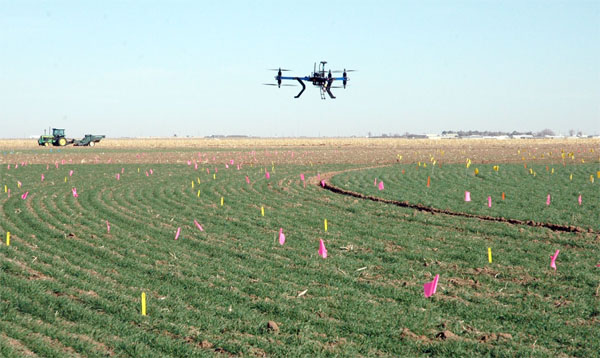
\includegraphics[width=0.7\linewidth, height=0.2\textheight]{Imagenes/dron_apli_1}
	\caption{Aplicaciones agr�colas con drones}
	\label{fig:dronapli1}
\end{figure}


\begin{figure}[h!]
	\centering
	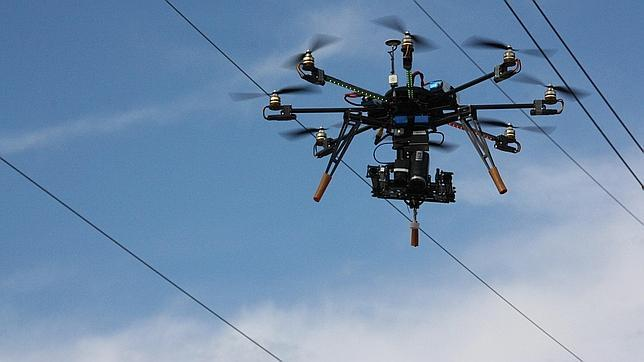
\includegraphics[width=0.7\linewidth, height=0.2\textheight]{Imagenes/drone_apli_2}
	\caption{Inspecci�n de tendido el�ctrico con drones}
	\label{fig:droneapli2}
\end{figure}

\begin{figure}[h!]
	\centering
	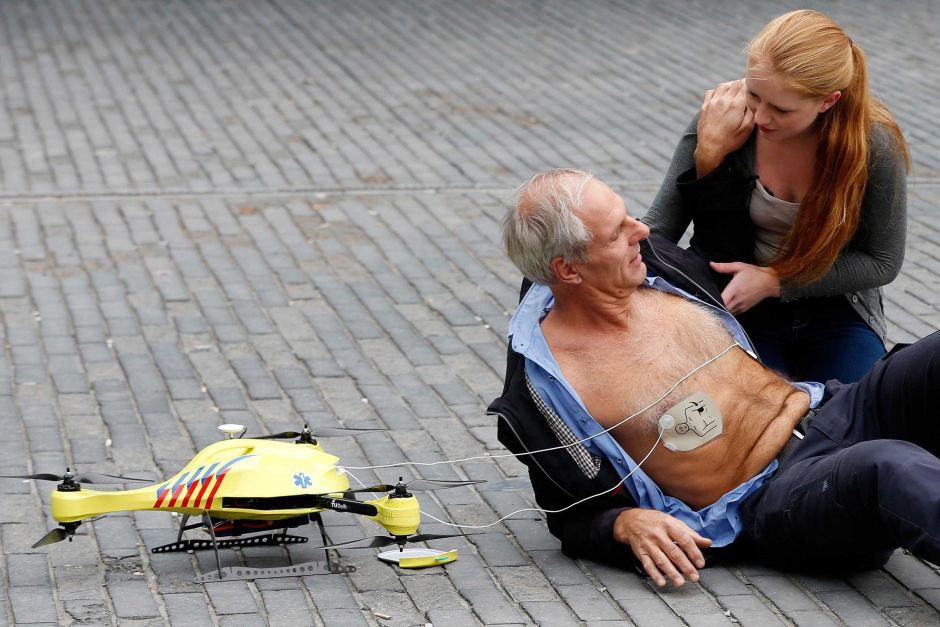
\includegraphics[width=0.7\linewidth, height=0.2\textheight]{Imagenes/dron_apli_rescue}
	\caption{Aplicaciones de emergencia}
	\label{fig:dronaplirescue}
\end{figure}

\begin{figure}[h!]
	\centering
	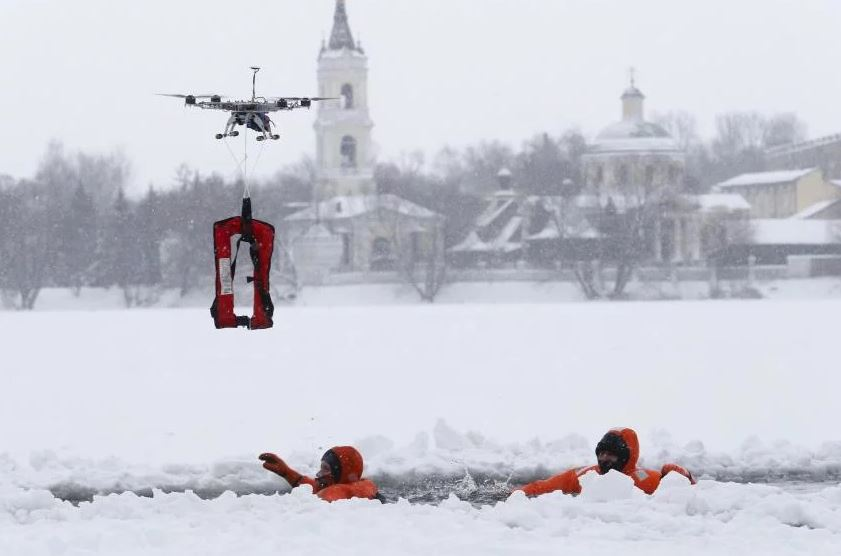
\includegraphics[width=0.7\linewidth, height=0.2\textheight]{Imagenes/dron_apli_rescue2}
	\caption{Aplicaciones de b�squeda y rescate}
	\label{fig:dronaplirescue2}
\end{figure}



Los UAVs pueden implementarse a trav�s de los dos tipos de veh�culos a�reos disponibles: aviones o multirotores (dentro de este �ltimo grupo se encuentran los cuadric�pteros). Esto hace que los UAVs resultantes presenten caracter�sticas din�micas y prestaciones (autonom�a, maniobrabilidad, capacidad de carga, etc.) muy definidas y diferentes. Los aviones son capaces de recorrer grandes distancias empleando poca energ�a, gracias a la sustentaci�n provista por las alas, de modo que el UAV resultante tiene una gran autonom�a. Sin embargo, las maniobras necesarias para relevar la informaci�n son muy complicadas o requieren de sistemas de control avanzados. Por otro lado, los
cuadric�pteros se caracterizan por su maniobrabilidad y su capacidad de vuelo estacionario (hovering), lo que los hace particularmente aptos para la recolecci�n de informaci�n en un punto determinado. Actualmente en el mercado nacional no se han reportado empresas que se dediquen al desarrollo de UAVs, siendo los mismos importados, tanto su hardware como su software. Por otro lado, los UAVs disponibles no son \textit{open source}, lo cual implica que la adaptaci�n de
los mismos a las necesidades de clientes y/o empresas se ve dificultada. Desde el punto de vista acad�mico-cient�fico, la posibilidad de implementar algoritmos propios en este tipo de veh�culos comerciales es pr�cticamente nula. Si bien existen empresas que se dedican al desarrollo de UAVs \textit{open source}, como lo es la empresa espa�ola Erle Robotics \footnote{P�gina web de Erle Robotics http://erlerobotics.com/}, pero los costos de adquisici�n de dichos veh�culos son bastante elevados. 
\par De lo expuesto anteriormente se desprende la necesidad de contar con una plataforma de desarrollo para UAVs. Una plataforma para este tipo de veh�culos, es un sistema que sirve como base para hacer funcionar los m�dulos de hardware o de software. En lo que concierne al hardware hacemos referencia a los componentes electr�nicos del UAVs como
pueden ser:
\begin{itemize}
	\item Motores.
	\item Sensores como aceler�metros, giroscopios, magnet�metros, etc.
	\item Perif�ricos de entrada y/o salida tales como tarjeta SD, puertos USB, entre otros.
\end{itemize}

Para poder obtener informaci�n de cada componente y gestionar sus interacciones es necesario que un software administre en un segundo plano estas tareas, y que de forma sencilla proporcione al usuario funcionalidades para manipular estos componentes electr�nicos, con el prop�sito de realizar acciones de navegaci�n sobre el veh�culo

% Lo dejo de manera general ya que van cambiando continuamente las acciones posibles
%, como pueden ser:

%\begin{itemize}
%	\item Despegar (Take off).
%	\item Mantenerse suspendido (hovering).
%	\item Desplazarse.
%\end{itemize}

Con el objetivo de solventar las deficiencias presentes en proyectos del mercado, tales como c�digo privativo y escasa visualizaci�n de datos en forma evolutiva, se propone realizar el proyecto \textit{open source} e implementar un m�dulo de visualizaci�n de datos a trav�s del tiempo, este tiene el prop�sito de monitorear y controlar las variables de estado y
controles del veh�culo. De esta forma, la realizaci�n del PFC propuesto ser� de gran utilidad para el desarrollo
de cualquier otro tipo de proyecto que involucre veh�culos aut�nomos, ya que facilitar� la tarea del operador para que el mismo enfoque su atenci�n en sus propios objetivos.
\par Para la realizaci�n del PFC, se tendr� a disposici�n el equipamiento e instalaciones del Instituto de Investigaci�n en Se�ales, Sistemas e Inteligencia Computacional (\textit{sinc(i)}), donde desempe�an sus actividades de investigaci�n los directores propuestos. El \textit{sinc(i) }fue creado en 2004 por la Facultad de Ingenier�a y Ciencias H�dricas (FICH) de la Universidad Nacional del Litoral (UNL), siendo reconocido como unidad ejecutora de doble dependencia UNL-CONICET en 2014. Las tareas de investigaci�n en el \textit{sinc(i)} tienen como objetivo desarrollar nuevos algoritmos para el aprendizaje autom�tico, procesamiento de se�ales, modelado y an�lisis de sistemas complejos, proporcionando tecnolog�as innovadoras para el avance de la salud, la agricultura de precisi�n, la bioinform�tica, la energ�a, los sistemas aut�nomos e interfaces hombre-m�quina. El \textit{sinc(i)} posee la infraestructura necesaria para el correcto desempe�o del PFC propuesto, a saber: espacio f�sico, equipamiento inform�tico, laboratorio de electr�nica, software, c�digos y algoritmos propios. Recientemente ha adquirido computadoras modelo Raspberry Pi \footnote{Computadora reducida en tama�o y de bajo coste https://www.raspberrypi.org/ } , que operan en conjunto con placas Navio2 \footnote{Placa electr�nica con un conjunto de sensores destinados para el control de navegaci�n.
 https://emlid.com/introducing-navio2/}, las cuales contienen GPS, doble IMU (unidad de medici�n inercial), gir�scopo y bar�metro, siendo de aplicaci�n espec�fica para navegaci�n de veh�culos aut�nomos. Adem�s, cuenta con un kit de GPS con soporte de RTK (los cuales logran precisi�n centim�trica) y con modelos a escala de un autom�vil tipo crawler y de un cuadric�ptero. Asimismo, posee un centro de prototipado r�pido que permite el desarrollo e implementaci�n de sistemas
embebidos a medida.
\par El desarrollo de este Proyecto Final de Carrera (PFC) impactar� positivamente tanto en la industria nacional como en el �mbito acad�mico, cient�fico y tecnol�gico. En primer lugar, el alumno adquirir� el know-how (experiencia, conocimiento y habilidad) en el manejo de sistemas embebidos para el desarrollo de plataformas \textit{open source} para UAVs. Adem�s, impulsar� el salto tecnol�gico no s�lo por el desarrollo de UAVs a nivel local con fines de entretenimiento, sino que tambi�n permitir� trasladar el conocimiento adquirido a la obtenci�n de UAVs con fines comerciales, econ�micos y/o sociales, entre otros, contribuyendo fuertemente al desarrollo de la industria argentina. Desde el punto de vista personal, la realizaci�n del PFC propuesto aumentar� el activo de conocimientos complementarios obtenidos en la carrera Ingenier�a en Inform�tica, ya que el mismo involucra temas relacionados como redes y comunicaci�n de datos, sistemas embebidos y electr�nica digital. Asimismo, contribuir� en la formaci�n pr�ctica y experimental, lo cual, en definitiva, es fundamental para el crecimiento de un profesional en este �mbito.

%------------------------------------------------------------------------
\section{Objetivos}
%------------------------------------------------------------------------

\begin{itemize}
	\item \textbf{Objetivo General}
		\subitem Instrumentar el cuadric�ptero con la Navio2 y la Raspberry Pi.
		\subitem Dise�ar e implementar una plataforma de desarrollo para UAVs.
	\item \textbf{Objetivos Espec�ficos}
		\subitem Desarrollar un m�dulo que permita la comunicaci�n inal�mbrica entre el
		cuadric�ptero y una PC para procesar la informaci�n adquirida.
		\subitem Desarrollar un m�dulo que permita la adquisici�n de datos relevantes como ser
		posici�n, velocidad, aceleraci�n y actitud.
		\subitem  Desarrollar un m�dulo de visualizaci�n de datos en tiempo real, el cual sea
		capaz de mostrar los datos provenientes de sensores que poseen alta
		frecuencia de muestreo.
		\subitem Evaluar el funcionamiento de la plataforma desarrollada mediante la utilizaci�n
		de un modelo a escala de un cuadric�ptero.
	
\end{itemize}



%------------------------------------------------------------------------
\section{Alcance}
%------------------------------------------------------------------------

El PFC propuesto consiste en desarrollar una plataforma para UAVs, que permita el control manual del mismo, adem�s que permita la visualizaci�n de forma gr�fica de los datos que fueron adquiridos de sus correspondientes sensores. Una vez desarrollada dicha plataforma ser� evaluada con un UAV tipo cuadric�ptero. El desarrollo del proyecto estar� restringido por las siguientes caracter�sticas:

\begin{itemize}
	\item La plataforma dispondr� del libre acceso al c�digo fuente, es decir, de tipo Open Source.
	\item Estar� orientado al uso de computadoras de escritorio.
	\item El lenguaje de codificaci�n utilizado ser� Python.
	\item Dispondr� de una interfaz gr�fica.
	\item Las opciones de navegaci�n que tendr� el cuadric�ptero moment�neamente ser�n:
		\subitem Punto objetivo.
		\subitem Aterrizar.
		\subitem Despegar.
		\subitem Estabilizarse.
		\subitem Volver al inicio.
\end{itemize}

En lo que concierne a las funcionalidades de la plataforma ser�n limitadas por los siguientes m�dulos:

	\subsection{M�dulo de operaci�n manual}
	
		El m�dulo perteneciente al control en modo manual ser� el encargado de gestionar los comandos que ser�n enviados desde un joystick conectado a la pc a nuestro cuadric�ptero. Estos comandos determinar�n los movimientos del veh�culo seg�n la restricci�n 5. 
		
	\subsection{M�dulo de comunicaci�n inal�mbrica}
		Corresponde a la comunicaci�n entre el ordenador y el cuadric�ptero. Se desarrollar� con tecnolog�a inal�mbrica, considerando un radio de cobertura seg�n los dispositivos disponibles a nuestro alcance. Adem�s, gestionar� el tipo de comunicaci�n entre el receptor y emisor, con eso hacemos referencia al protocolo de comunicaci�n, velocidad de transferencia, entre otros. Por el mismo medio se transmitir�n los datos obtenidos por los 	sensores como tambi�n las maniobras establecidas por el usuario de forma manual.
	
	\subsection{M�dulo de gr�fico de datos}
	
		Este m�dulo permitir� la selecci�n del sensor de nuestro inter�s, y mostrar� de forma gr�fica c�mo evolucionan los datos que se est�n obteniendo de los mismos en tiempo real.	Debido a que la mayor�a de los sensores utilizados emplean una frecuencia de muestreo alta, es necesario utilizar librer�as gr�ficas que sean capaces de cumplir con los 	requerimientos de tiempo real. Para asegurar este objetivo, se propone utilizar VisPy o	similar, la cual es una librer�a escrita en lenguaje Python que est� dise�ada espec�ficamente para la visualizaci�n interactiva de gran cantidad de datos de forma r�pida, escalable y f�cil. Con respecto a la adquisici�n de datos de los sensores, en el mercado existe un sinf�n de �stos que son de utilidad para alg�n problema que se quiera resolver, como podr�an ser:	detecci�n de temperatura, presi�n, humo, obtenci�n de im�genes mediante una c�mara o la	captura de un video, entre otros. 
		\par En este PFC se utilizar�n los sensores que nos proporciona la placa Navio2, a saber:
		
		\begin{itemize}
			\item  2 unidades de medici�n inercial MPU 9250 9DOF y LSM9DS1 9DOF. Son dispositivos electr�nicos que miden e informan acerca de la velocidad, orientaci�n y fuerzasmagn�ticas utilizando una combinaci�n de aceler�metros y gir�scopos.
			\item 1 bar�metro MS5611 para medir la presi�n atmosf�rica.
			\item 1 sistema de navegaci�n por sat�lite U-blox M8N, el cual utilizan una combinaci�n delas tecnolog�as Glonass/GPS/Beidou.
		\end{itemize}
	Los cuales ser�n detallados en los pr�ximos cap�tulos. 

% TODO: Consultar si se puede dejar las actividades



% Variable local para emacs, para  que encuentre el fichero maestro de
% compilaci�n y funcionen mejor algunas teclas r�pidas de AucTeX
%%%
%%% Local Variables:
%%% mode: latex
%%% TeX-master: "../ManualTeXiS.tex"
%%% End:
    % JOA
% -*-coding: iso-latin-1  -*-
%---------------------------------------------------------------------
%
%                          Cap�tulo 1
%
%---------------------------------------------------------------------
%
% 01Introduccion.tex
% Copyright 2009 Marco Antonio Gomez-Martin, Pedro Pablo Gomez-Martin
%
% This file belongs to the TeXiS manual, a LaTeX template for writting
% Thesis and other documents. The complete last TeXiS package can
% be obtained from http://gaia.fdi.ucm.es/projects/texis/
%
% Although the TeXiS template itself is distributed under the 
% conditions of the LaTeX Project Public License
% (http://www.latex-project.org/lppl.txt), the manual content
% uses the CC-BY-SA license that stays that you are free:
%
%    - to share & to copy, distribute and transmit the work
%    - to remix and to adapt the work
%
% under the following conditions:
%
%    - Attribution: you must attribute the work in the manner
%      specified by the author or licensor (but not in any way that
%      suggests that they endorse you or your use of the work).
%    - Share Alike: if you alter, transform, or build upon this
%      work, you may distribute the resulting work only under the
%      same, similar or a compatible license.
%
% The complete license is available in
% http://creativecommons.org/licenses/by-sa/3.0/legalcode
%
%---------------------------------------------------------------------

%\chapter{Justificaci�n, Objetivos y Alcance}
\chapter{Introducci�n}

\begin{FraseCelebre}
\begin{Frase}
Primer paso, debes tener un definitivo y claro objetivo. Segundo, debes tener los recursos necesarios para alcanzar lo que deseas; sabidur�a, dinero, recursos y m�todos. Tercero, enfoca todos tus recursos para el logro de tus metas.

\end{Frase}
\begin{Fuente}
	-Arist�teles-
\end{Fuente}
\end{FraseCelebre}

\begin{resumen}
En este cap�tulo se detallan los elementos que dan origen a este proyecto y componen la especificaci�n del mismo. Se hace una rese�a de los antecedentes identificados y c�mo se justifica el trabajo realizado, aclarando los objetivos planteados para ellos y las restricciones tenidas en cuenta para el alcance y las tecnolog�as utilizadas. 
\end{resumen}

\newpage
%-------------------------------------------------------------------
\section{Justificaci�n}
%-------------------------------------------------------------------
\label{cap0:sec:justificacion}


Una de las �reas de la aviaci�n que ha experimentado un r�pido crecimiento es aquella relacionada con los veh�culos a�reos no tripulados (del ingl�s unmanned aerial vehicle UAV). Esta clase de veh�culos pueden ser operados de forma remota o totalmente aut�noma, presentan reducidos costos de operaci�n \cite{valavanis2008unmanned,valavanis2008advances} y adem�s no ponen en riesgo al operador. En los �ltimos a�os han ganado gran inter�s debido a su utilizaci�n en misiones de b�squeda y rescate \cite{doherty2007uav}, inspecci�n de l�neas el�ctricas \cite{jones2005power}, actividades agr�colas \cite{zhang2012application}, recolecci�n de im�genes \cite{adams2013high}, seguridad \cite{maza2011experimental}, lucha contra incendios forestales \cite{maza2011experimental,ollero2006unmanned}, entre otros.

\begin{figure}[h!]
	\centering
	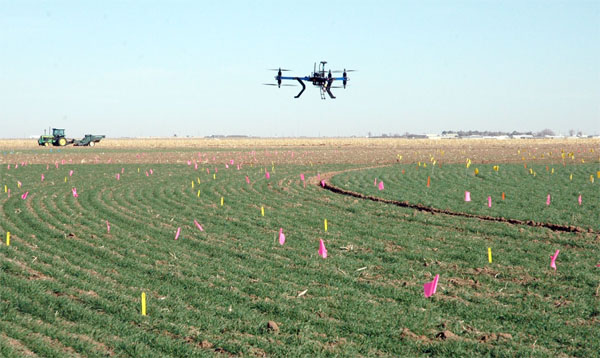
\includegraphics[width=0.7\linewidth, height=0.2\textheight]{Imagenes/dron_apli_1}
	\caption{Aplicaciones agr�colas con drones}
	\label{fig:dronapli1}
\end{figure}


\begin{figure}[h!]
	\centering
	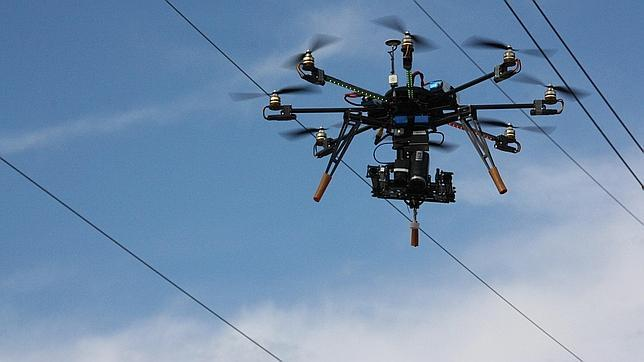
\includegraphics[width=0.7\linewidth, height=0.2\textheight]{Imagenes/drone_apli_2}
	\caption{Inspecci�n de tendido el�ctrico con drones}
	\label{fig:droneapli2}
\end{figure}

\begin{figure}[h!]
	\centering
	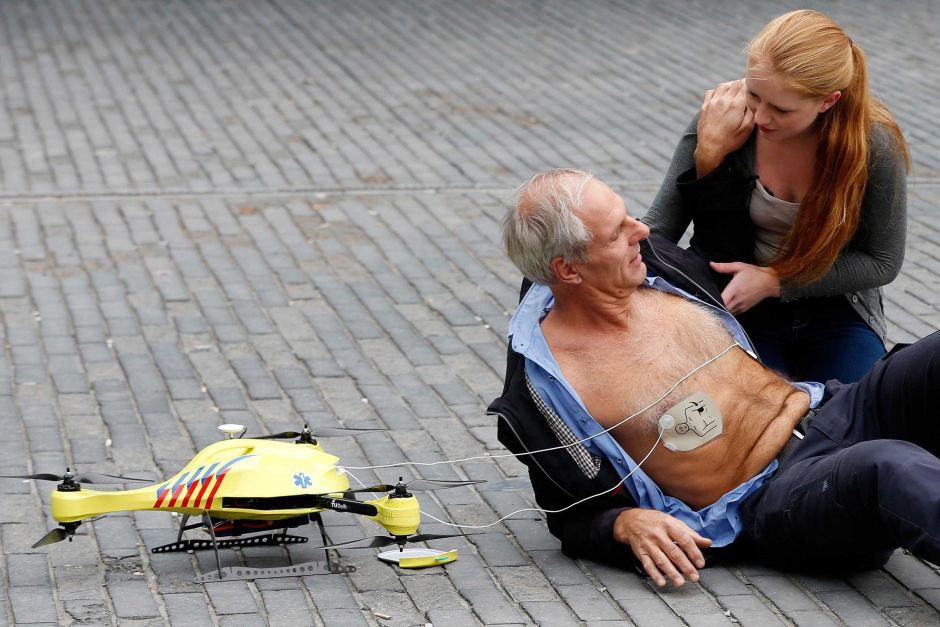
\includegraphics[width=0.7\linewidth, height=0.2\textheight]{Imagenes/dron_apli_rescue}
	\caption{Aplicaciones de emergencia}
	\label{fig:dronaplirescue}
\end{figure}

\begin{figure}[h!]
	\centering
	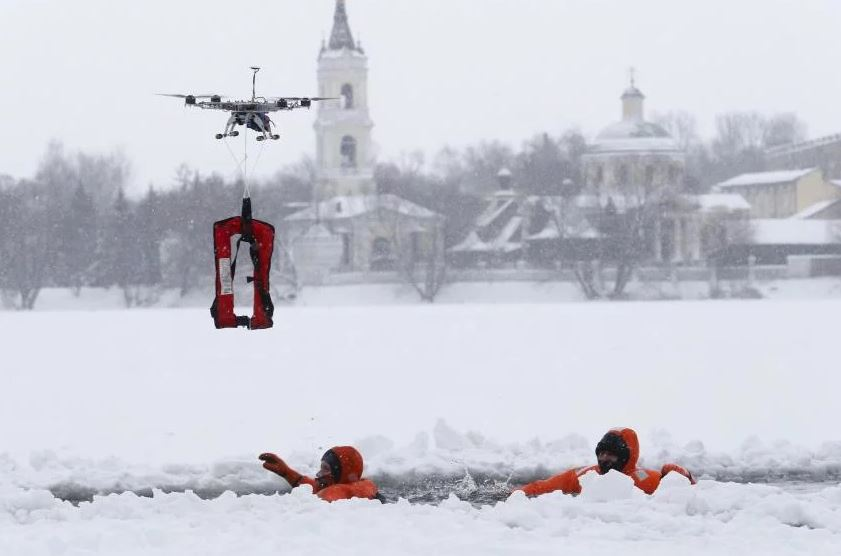
\includegraphics[width=0.7\linewidth, height=0.2\textheight]{Imagenes/dron_apli_rescue2}
	\caption{Aplicaciones de b�squeda y rescate}
	\label{fig:dronaplirescue2}
\end{figure}



Los UAVs pueden clasificarse en varios tipos, en nuestro caso nos centraremos exclusivamente en los tipos de veh�culos en funci�n de su tipo de sustentaci�n, como pueden ser: UAVs de ala fija o rotatoria.
\newline \newline \textbf{UAV de ala fija} \newline
\par Los UAVs de ala fija son aeronaves que poseen un perfil alar que permite que la aeronave pueda moverse a trav�s del aire y sea capaz de generar fuerzas sustentadoras para mantenerse en el aire. Este tipo de veh{iculo tienen una est�tica muy similar a los aeromodelos de radiocontrol. La principal caracter�stica de este tipo, es la gran autonom�a que nos ofrecen ya que pueden estar volando varias horas gracias a su 
eficiencia aerodin�mica. Estos son ideales para mapear grandes superficies de terreno ya que con una �nica bater�a se cubren  grandes extensiones de terreno. Por este motivo son muy utilizados en trabajos de agricultura de precisi�n y de fotogrametr�a. A diferencia de los UAVs de ala rotatoria, con este tipo no es posible realizar vuelos estacionarios. Por tanto, no podremos realizar trabajos que requieran que el veh�culo este volando fijo a una altura determinada como pueden ser, por ejemplo, los trabajos de inspecci�n. Otra particularidad de este tipo es que no pueden despegar ni aterrizar en vertical. Para el despegue de necesitaremos una persona que se encargue de lanzarlo a mano o disponer directamente de una catapulta. 
\newline \newline \textbf{UAV de ala rotatoria}\newline
 \par Los UAVs de ala rotatoria, o m�s conocidos como multirrotores, son lo tipos m�s extendidos y m�s utilizados por los profesionales del sector.  La principal diferencia de los multirrotores con respecto a los UAVs de ala fija radica en la forma en la que consiguen mantenerse en el aire.  Mientras que los veh�culos de ala fija consiguen la sustentaci�n a trav�s de su perfil alar, los multirrotores generan la sustentaci�n a trav�s de  las fuerzas que generan las h�lices de sus rotores. Seg�n el n�mero rotores que monte el veh�culo existen: tric�pteros (3 motores), cuadric�pteros (4 motores), hexac�pteros (6 motores) y octac�pteros 
 (8 motores).  La principal caracter�sticas de los multirrotores es su versatilidad. De una forma sencilla se le pueden instalar diferentes tipos de c�maras  (c�maras RGB, multiespectrales, termogr�ficas, etc) que nos permiten realizar un gran abanico de trabajos. Adem�s, con este tipo de UAV vamos a  poder realizar vuelos estacionarios lo que nos va a permitir realizar ciertos trabajos que con uno de ala fija ser�a imposible realizar.
 \par Actualmente en el mercado nacional no se han reportado empresas que se dediquen al desarrollo de UAVs, siendo los mismos importados, tanto su hardware como su software. Por otro lado, los UAVs disponibles no son  de c�digo abierto, lo cual implica que la adaptaci�n de
los mismos a las necesidades de clientes y/o empresas se ve dificultada. Desde el punto de vista acad�mico-cient�fico, la posibilidad de implementar algoritmos propios en este tipo de veh�culos comerciales es pr�cticamente nula. Si bien existen empresas que se dedican al desarrollo de UAVs de c�digo abierto, como lo es la empresa espa�ola Erle Robotics\footnote{P�gina web de Erle Robotics http://erlerobotics.com/}, pero los costos de adquisici�n de dichos veh�culos son bastante elevados. 
\par De lo expuesto anteriormente se desprende la necesidad de contar con una plataforma de desarrollo para UAVs. Una plataforma para este tipo de veh�culos, es un sistema que sirve como base para hacer funcionar los m�dulos de hardware o de software. En lo que concierne al hardware hacemos referencia a los componentes electr�nicos del UAV como pueden ser:
\begin{itemize}
	\item Motores.
	\item Sensores como aceler�metros, giroscopios, magnet�metros, etc.
	\item Perif�ricos de entrada y/o salida tales como tarjeta SD, puertos \ac{USB}, entre otros.
\end{itemize}

Para poder obtener informaci�n de cada componente y gestionar sus interacciones es necesario que un software administre en un segundo plano estas tareas, y que de forma sencilla proporcione al usuario funcionalidades para manipular estos componentes electr�nicos, con el prop�sito de realizar acciones de navegaci�n sobre el veh�culo

% Lo dejo de manera general ya que van cambiando continuamente las acciones posibles
%, como pueden ser:

%\begin{itemize}
%	\item Despegar (Take off).
%	\item Mantenerse suspendido (hovering).
%	\item Desplazarse.
%\end{itemize}

Con el objetivo de solventar las deficiencias presentes en proyectos del mercado, tales como c�digo privativo y escasa visualizaci�n de datos en forma evolutiva, se propone realizar el proyecto de c�digo abierto e implementar un m�dulo de visualizaci�n de datos a trav�s del tiempo, con el prop�sito de monitorear y controlar las variables de estado y
controles del veh�culo. De esta forma, la realizaci�n del Proyecto Final de Carrera (PFC) propuesto ser� de gran utilidad para el desarrollo
de cualquier otro tipo de proyecto que involucre veh�culos aut�nomos, ya que facilitar� la tarea del operador para que el mismo enfoque su atenci�n en sus propios objetivos.
\par Para la realizaci�n del PFC, se tendr� a disposici�n el equipamiento e instalaciones del Instituto de Investigaci�n en Se�ales, Sistemas e Inteligencia Computacional (\textit{sinc(i)}), donde desempe�an sus actividades de investigaci�n los directores propuestos. El \textit{sinc(i) }fue creado en 2004 por la Facultad de Ingenier�a y Ciencias H�dricas (FICH) de la Universidad Nacional del Litoral (UNL), siendo reconocido como unidad ejecutora de doble dependencia UNL-CONICET en 2014. Las tareas de investigaci�n en el sinc(i) tienen como objetivo desarrollar nuevos algoritmos para el aprendizaje autom�tico, procesamiento de se�ales, modelado y an�lisis de sistemas complejos, proporcionando tecnolog�as innovadoras para el avance de la salud, la agricultura de precisi�n, la bioinform�tica, la energ�a, los sistemas aut�nomos e interfaces hombre-m�quina. El \textit{sinc(i)} posee la infraestructura necesaria para el correcto desempe�o del PFC propuesto, a saber: espacio f�sico, equipamiento inform�tico, laboratorio de electr�nica, software, c�digos y algoritmos propios. Recientemente ha adquirido computadoras modelo Raspberry Pi\footnote{Computadora reducida en tama�o y de bajo coste https://www.raspberrypi.org/ } , que operan en conjunto con placas Navio2\footnote{Placa electr�nica con un conjunto de sensores destinados para el control de navegaci�n.
 https://emlid.com/introducing-navio2/}, las cuales contienen GPS, doble IMU (unidad de medici�n inercial), magnet�metro y bar�metro, siendo de aplicaci�n espec�fica para navegaci�n de veh�culos aut�nomos. Adem�s, cuenta con un kit de GPS con soporte de RTK (los cuales logran precisi�n centim�trica) y con modelos a escala de un autom�vil tipo crawler y de un cuadric�ptero. Asimismo, posee un centro de prototipado r�pido que permite el desarrollo e implementaci�n de sistemas
embebidos a medida.
\par El desarrollo de este PFC impactar� positivamente tanto en la industria nacional como en el �mbito acad�mico, cient�fico y tecnol�gico. En primer lugar, el alumno adquirir� el know-how (experiencia, conocimiento y habilidad) en el manejo de sistemas embebidos para el desarrollo de plataformas de c�digo abierto para UAVs. Adem�s, impulsar� el salto tecnol�gico no s�lo por el desarrollo de UAVs a nivel local con fines de entretenimiento, sino que tambi�n permitir� trasladar el conocimiento adquirido a la obtenci�n de UAVs con fines comerciales, econ�micos y/o sociales, entre otros, contribuyendo fuertemente al desarrollo de la industria argentina. Desde el punto de vista personal, la realizaci�n del PFC propuesto aumentar� el activo de conocimientos complementarios obtenidos en la carrera Ingenier�a en Inform�tica, ya que el mismo involucra temas relacionados como redes y comunicaci�n de datos, sistemas embebidos y electr�nica digital. Asimismo, contribuir� en la formaci�n pr�ctica y experimental, lo cual, en definitiva, es fundamental para el crecimiento de un profesional en este �mbito.

%------------------------------------------------------------------------
\section{Objetivos}
%------------------------------------------------------------------------

\begin{itemize}
	\item \textbf{Objetivo General}
		\subitem Instrumentar el cuadric�ptero con la placa de autopiloto Navio2 y el ordenador de placa reducida Raspberry Pi.
		\subitem Dise�ar e implementar una plataforma de desarrollo para UAVs.
	\item \textbf{Objetivos Espec�ficos}
		\subitem Desarrollar un m�dulo que permita la comunicaci�n inal�mbrica entre el
		cuadric�ptero y una \ac{PC} para procesar la informaci�n adquirida.
		\subitem Desarrollar un m�dulo que permita la adquisici�n de datos relevantes como ser
		posici�n, velocidad, aceleraci�n y actitud.
		\subitem  Desarrollar un m�dulo de visualizaci�n de datos en tiempo real, el cual sea
		capaz de mostrar los datos provenientes de sensores que poseen alta
		frecuencia de muestreo.
		\subitem Evaluar el funcionamiento de la plataforma desarrollada mediante la utilizaci�n
		de un modelo a escala de un cuadric�ptero.
	
\end{itemize}



%------------------------------------------------------------------------
\section{Alcance}
%------------------------------------------------------------------------

El PFC propuesto consiste en desarrollar una plataforma para UAVs, que permita el control manual del mismo, adem�s que permita la visualizaci�n de forma gr�fica de los datos que fueron adquiridos de sus correspondientes sensores. Una vez desarrollada dicha plataforma ser� evaluada con un UAV tipo cuadric�ptero. El desarrollo del proyecto estar� restringido por las siguientes caracter�sticas:

\begin{enumerate}
	\item La plataforma dispondr� del libre acceso al c�digo fuente, es decir, de tipo c�digo abierto distribuyendose bajo la licencia del MIT.\footnote{Repositorio del proyecto https://github.com/ERicBastida/BEcopter }
	\item Estar� orientado al uso de computadoras de escritorio.
	\item El lenguaje de codificaci�n utilizado ser� Python.
	\item Dispondr� de una interfaz gr�fica.
	\item Las opciones de navegaci�n que tendr� el cuadric�ptero ser�n:
		\subitem Ir a punto objetivo.
		\subitem Aterrizar.
		\subitem Despegar.
		\subitem Estabilizarse.
		\subitem Volver al inicio.
\end{enumerate}

En lo que concierne a las funcionalidades de la plataforma ser�n limitadas por los siguientes m�dulos:

	\subsection{M�dulo de operaci�n manual}
	
		El m�dulo perteneciente al control en modo manual ser� el encargado de gestionar los comandos que ser�n enviados a nuestra cuadric�ptero desde un joystick conectado a la PC. Estos comandos determinar�n los movimientos del veh�culo seg�n la restricci�n 5. 
		
	\subsection{M�dulo de comunicaci�n inal�mbrica}
		Corresponde a la comunicaci�n entre la PC y el cuadric�ptero. Se desarrollar� con tecnolog�a inal�mbrica, considerando un radio de cobertura seg�n los dispositivos disponibles a nuestro alcance. Adem�s, gestionar� el tipo de comunicaci�n entre el receptor y emisor, con eso hacemos referencia al protocolo de comunicaci�n, velocidad de transferencia, entre otros. Por el mismo medio se transmitir�n los datos obtenidos por los 	sensores como tambi�n las maniobras establecidas por el usuario de forma manual.
	
	\subsection{M�dulo de gr�fico de datos}
	
		Este m�dulo permitir� la selecci�n del sensor de nuestro inter�s, y mostrar� de forma gr�fica c�mo evolucionan los datos que se est�n obteniendo de los mismos en tiempo real.	Debido a que la mayor�a de los sensores utilizados emplean una frecuencia de muestreo alta, es necesario utilizar bibliotecas gr�ficas que sean capaces de cumplir con los 	requerimientos de tiempo real. Para asegurar este objetivo, se propone utilizar VisPy\footnote{P�gina web vispy.org} o	similar, la cual est� escrita en Python y dise�ada espec�ficamente para la visualizaci�n interactiva de gran cantidad de datos en forma r�pida, escalable y sencillo. Con respecto a la adquisici�n de datos de los sensores, en el mercado existe un sinf�n de �stos que son de utilidad para alg�n problema que se quiera resolver, como podr�an ser:	detecci�n de temperatura, presi�n, humo, obtenci�n de im�genes mediante una c�mara o la	captura de un video, entre otros. 
		\par En este PFC se utilizar�n los sensores que nos proporciona la placa Navio2, a saber:
		
		\begin{itemize}
			\item  2 unidades de medici�n inercial \ac{MPU} 9250 9DOF y LSM9DS1 9DOF. Son dispositivos electr�nicos que miden e informan acerca de la velocidad, orientaci�n y fuerzas magn�ticas utilizando una combinaci�n de aceler�metros, gir�scopos y magnet�metros.
			\item 1 bar�metro MS5611 para medir la presi�n atmosf�rica.
			\item 1 sistema de navegaci�n por sat�lite U-blox M8N, el cual utiliza una combinaci�n de las tecnolog�as Glonass/\ac{GPS}/Beidou.
		\end{itemize}


% TODO: Consultar si se puede dejar las actividades



% Variable local para emacs, para  que encuentre el fichero maestro de
% compilaci�n y funcionen mejor algunas teclas r�pidas de AucTeX
%%%
%%% Local Variables:
%%% mode: latex
%%% TeX-master: "../ManualTeXiS.tex"
%%% End:
    % Obtencion de los requerimientos
%---------------------------------------------------------------------
%
%                          Cap�tulo 2
%
%---------------------------------------------------------------------
%
% 02EstructuraYGeneracion.tex
% Copyright 2009 Marco Antonio Gomez-Martin, Pedro Pablo Gomez-Martin
%
% This file belongs to the TeXiS manual, a LaTeX template for writting
% Thesis and other documents. The complete last TeXiS package can
% be obtained from http://gaia.fdi.ucm.es/projects/texis/
%
% Although the TeXiS template itself is distributed under the 
% conditions of the LaTeX Project Public License
% (http://www.latex-project.org/lppl.txt), the manual content
% uses the CC-BY-SA license that stays that you are free:
%
%    - to share & to copy, distribute and transmit the work
%    - to remix and to adapt the work
%
% under the following conditions:
%
%    - Attribution: you must attribute the work in the manner
%      specified by the author or licensor (but not in any way that
%      suggests that they endorse you or your use of the work).
%    - Share Alike: if you alter, transform, or build upon this
%      work, you may distribute the resulting work only under the
%      same, similar or a compatible license.
%
% The complete license is available in
% http://creativecommons.org/licenses/by-sa/3.0/legalcode
%
%---------------------------------------------------------------------

% -------------------------------------------------------------------------------
%      Estilos para los segmentos de c�digos/comandos para aparentar una consola
% -------------------------------------------------------------------------------

\definecolor{gray97}{gray}{.97}
\definecolor{gray75}{gray}{.75}
\definecolor{gray45}{gray}{.45}

\definecolor{mygray}{rgb}{0.4,0.4,0.4}
\definecolor{mygreen}{rgb}{0,0.8,0.6}
\definecolor{myorange}{rgb}{1.0,0.4,0}
\definecolor{gray97}{gray}{.97}
\definecolor{gray75}{gray}{.75}
\definecolor{gray45}{gray}{.45}

\lstset{ 
	basicstyle=\footnotesize\sffamily\color{black},
	commentstyle=\color{mygray},
	frame=single,
	numbers=left,
	numbersep=5pt,
	numberstyle=\tiny\color{mygray},
	keywordstyle=\color{mygreen},
	showspaces=false,
	showstringspaces=false,
	stringstyle=\color{myorange},
	tabsize=2
}

% minimizar fragmentado de listados
\lstnewenvironment{listing}[1][]
{\lstset{#1}\pagebreak[0]}{\pagebreak[0]}

\lstdefinestyle{consola}
{basicstyle=\scriptsize\bf\ttfamily,
	backgroundcolor=\color{gray75},
}

\lstdefinestyle{Python}
{language=Python,
}


\lstset{ frame=Ltb,
	framerule=0pt,
	aboveskip=0.5cm,
	framextopmargin=3pt,
	framexbottommargin=4pt,
	framexleftmargin=0.4cm,
	framesep=0pt,
	rulesep=.4pt,
	backgroundcolor=\color{gray97},
	rulesepcolor=\color{black},
	%
	stringstyle=\ttfamily,
	showstringspaces = false,
	basicstyle=\small\ttfamily,
	commentstyle=\color{gray45},
	keywordstyle=\bfseries,
	%
	numbers=left,
	numbersep=15pt,
	numberstyle=\tiny,
	numberfirstline = false,
	breaklines=true,
}

\lstdefinestyle{consola}
{basicstyle=\scriptsize\bf\ttfamily,
	backgroundcolor=\color{gray75},
}




\chapter{Gesti�n de componentes y armado del cuadric�ptero}
\label{cap2:gest_y_arm}

\begin{FraseCelebre}
	
	\begin{Frase}
	 La mejor estructura no garantizar� los resultados ni el rendimiento.
	 Pero la estructura equivocada es una garant�a de fracaso.
	\end{Frase}

	\begin{Fuente}
		Peter Drucker
	\end{Fuente}

\end{FraseCelebre}

\begin{resumen}
Este cap�tulo contiene informaci�n sobre el procedimiento que se ha llevado a cabo en el desarrollo de la tercera etapa del proyecto. Esta etapa consiste principalmente en describir los pasos realizados para el armado del veh�culo a�reo no tripulado (VANT) de tipo cuadric�ptero. Adem�s, se incluir�n los inconvenientes que se han presentado en el transcurso del desarrollo del mismo con sus respectivas alternativas y/o soluciones. 

% TODO: Consultar si dejar esta parte   
\par Cabe mencionar que el hardware aqu� descripto como tambi�n las herramientas utilizadas han sido proporcionadas por el\textit{ Centro de Investigaci�n en Se�ales, Sistemas e Inteligencia sinc(i)} con sede en la Facultad de Ingenier�a y Ciencias H�dricas de la Universidad Nacional del Litoral y todo procedimiento riesgoso para el alumno ha sido siempre supervisado bajo personal id�neo en el tema.

\end{resumen}

%-------------------------------------------------------------------
\section{Hardware}
%-------------------------------------------------------------------
\label{cap2:sec:hardware}

Antes de empezar con la descripci�n del armado de un VANT, es necesario tener en conocimiento el hardware que est� involucrado en el veh�culo y en consecuencia su funcionamiento, como por ejemplo, los sensores que forman parte del mismo y hacen que el cuadric�ptero pueda realizar un vuelo de manera segura y controlada, el tipo de estructura usado para soportar los motores, la tecnolog�a responsable de la comunicaci�n y el ordenador que procesar� toda esa informaci�n. Es por eso que iniciamos esta secci�n con una lista del hardware utilizado y su respectiva descripci�n:


\begin{enumerate}
	\item Estructura de veh�culo.
	\item Controlador Electr�nico de Velocidad.
	\item Motor sin escobillas.
	\item Raspberry Pi 3.
	\item Navio2.
	\item Arduino UNO \footnote{Estos dispositivos no han sido previstos y tampoco forman parte definitiva del proyecto, ya que han surgido para solventar problemas que surgieron en el transcurso de esta etapa. \label{footnote_hardware} }.
	\item Radio Control \footref{footnote_hardware}.
	\item Joystick.
	\item Router \footref{footnote_hardware}.
	\item M�dulos XBee
	\item Bateria LiPo.
\end{enumerate}




	\subsection{Estructura de veh�culo}

		La estructura del cuadric�ptero como se puede ver en la Figura \ref{fig:estrucuadricoptero} consta en su parte inferior de un pat�n de aterrizaje que cumplen la funci�n (como en los helic�pteros) de soportar el veh�culo cuando se apoye sobre tierra y mantener las h�lices lo m�s alejado posible de piso cuando se encuentra en reposo. En su parte superior proporciona una base donde es posible instalar los dispositivos electr�nicos que controlan al veh�culo. Por �ltimo, desde la base se extienden 4 brazos con la funci�n de ser soporte a los motores con sus respectivas h�lices y adem�s, en cada motor se le incluye su controlador electr�nico de velocidad o ESC (\textit{Electronic Speed Controller}). 




		\begin{figure}[h!]
			\centering
			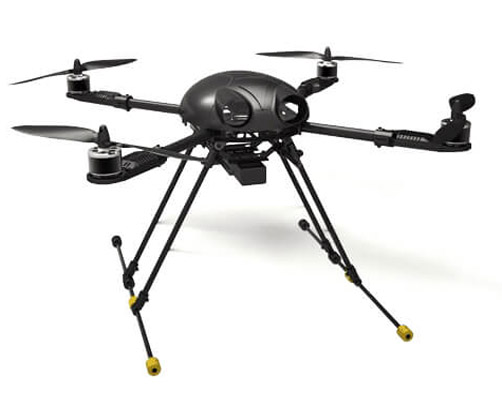
\includegraphics[width=0.4\linewidth, height=0.25\textheight]{Imagenes/estrucuadricoptero}
			\caption{Estructura cuadric�ptero de fibra de carbono}
			\label{fig:estrucuadricoptero}
		\end{figure}

		El material del cuerpo de veh�culo esta hecho con fibra de carbono \footnote{Aunque el mismo puede ser reemplazado por otro tipo de estructura, por ejemplo, un modelo impreso por una impresora 3D}, este consta con la propiedad de tener una elevada resistencia mec�nica que ser� de suma importancia ya que el veh�culo presenta altas probabilidades de sufrir alg�n choque o aterrizaje forzoso, adem�s de ser un material sumamente liviano por lo que disminuir� la fuerza de los motores para mantener un vuelo y por tanto, menos consumo de bater�a.
		

	\subsection{Controlador Electr�nico de Velocidad}
		Un controlador electr�nico de velocidad o por sus siglas en ingl�s \textit{Electronic Speed Control} como su nombre lo dice, es un circuito electr�nico con el prop�sito de variar la velocidad de un motor el�ctrico. Adem�s, por sus caracter�sticas puede funcionar como un freno din�mico.

		\begin{figure}[h!]
			\centering
			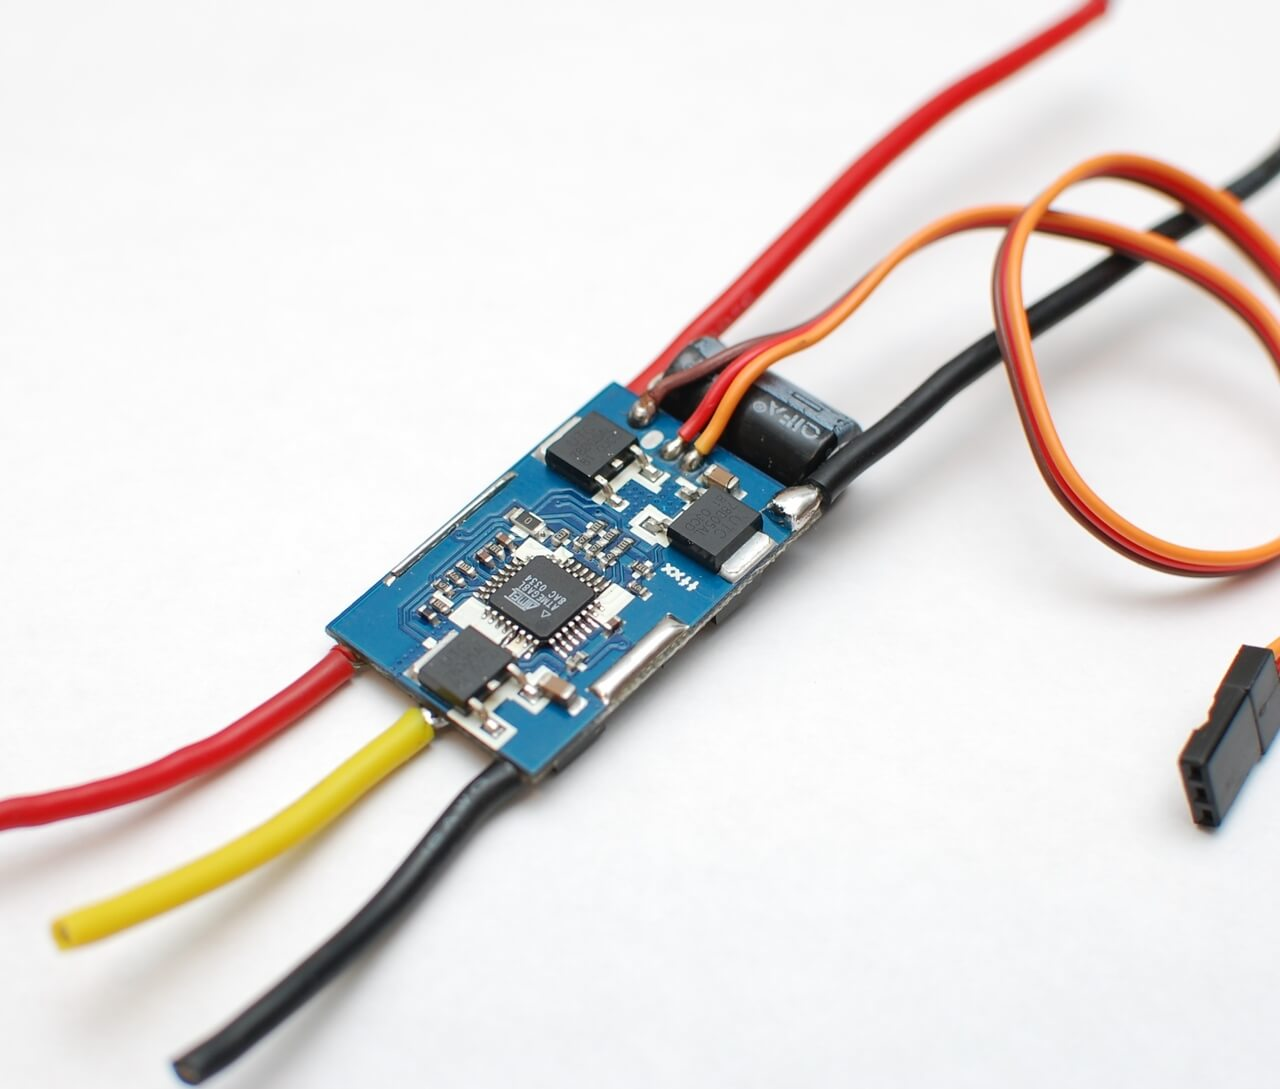
\includegraphics[width=0.4\linewidth, height=0.1\textheight]{Imagenes/esc}
			\caption{Controlador Electr�nico de Velocidad}
			\label{fig:esc}
		\end{figure}

	\subsection{Motores sin escobillas}
		Son los encargados de transformar la energ�a el�ctrica en mec�nica generando movimiento en las h�lices, y de esta manera dando propulsi�n al veh�culo para poder volar.

		\begin{figure}[h!]
			\centering
			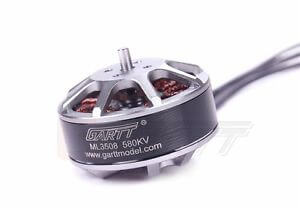
\includegraphics[width=0.4\linewidth, height=0.15\textheight]{Imagenes/motor}
			\caption{Motor sin escobillas}
			\label{fig:motor}
		\end{figure}

	\subsection{Raspberry Pi 3}
		Es un ordenador de tama�o reducido que trata de ofrecer las mismas funcionalidades y componentes que el de un ordenador com�n pero con un rendimiento menor, entre sus componentes, esta placa reducida tiene memoria RAM, GPU, puertos USB, HDMI, ranura para tarjeta SD, conector para una c�mara, conectividad WiFi, Ethernet, Bluetooth y 40 pines GPIO(\textit{General Purpose Input/Output}) donde es posible extender sus caracter�sticas instalando hardware extra como sensores, led, motores, interfaces, etc.\par \textbf{Especificaciones:}
		\begin{itemize}
			
			\item 1.2GHz 64-bit quad-core ARMv8 CPU
			\item 1GB RAM (Compartido con la GPU)
			\item GPU Broadcom VideoCore IV	\newline
		\end{itemize}
		
		\begin{figure}[h!]
			\centering
			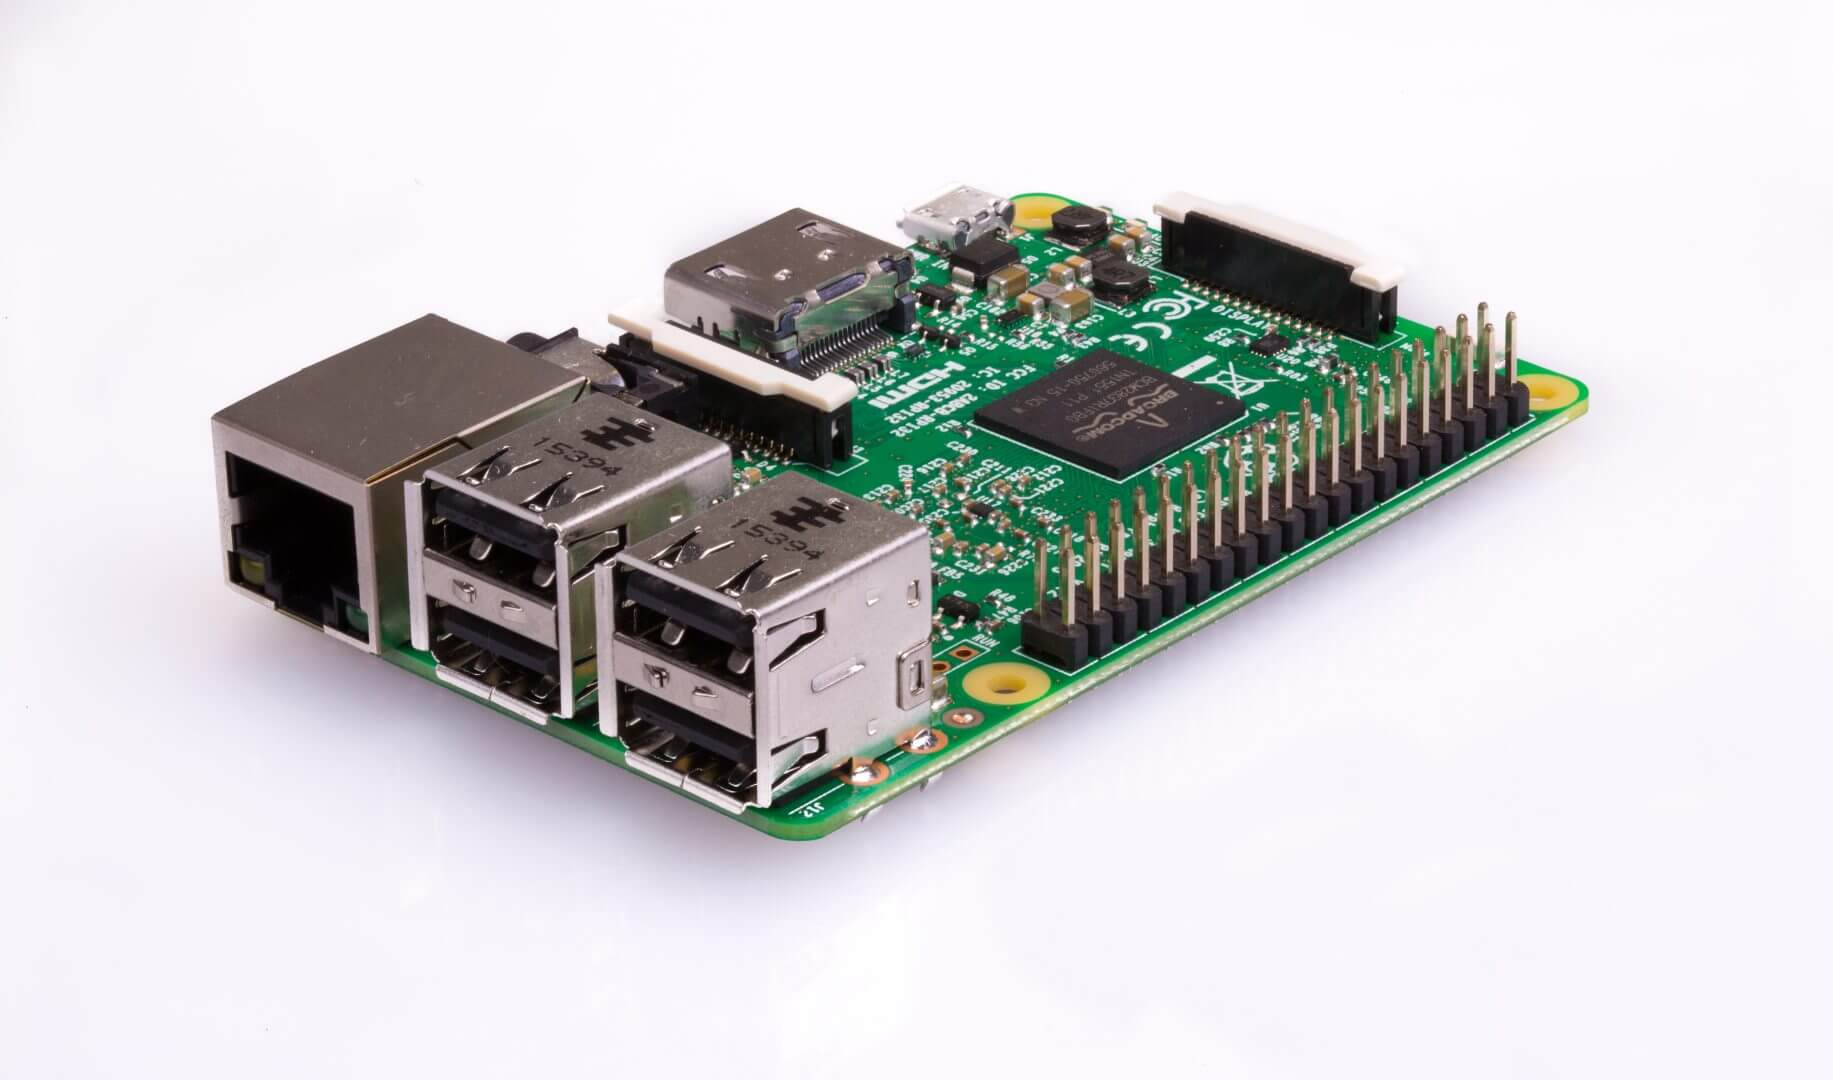
\includegraphics[width=0.6\linewidth]{Imagenes/raspberry3}
			\caption{Raspberry Pi 3}
			\label{fig:raspberry3}
		\end{figure}


	\subsection{Navio2}
		La placa Navio2 es un conjunto de sensores que se conectan sobre pines GPIO de una Raspberry Pi, transform�ndolo en un completo controlador de drones. Esta placa controladora suministra a la Raspberry Pi de sensores y entradas que son de suma importancia para cualquier tipo de veh�culo, con el objetivo de monitorear y obtener informaci�n para alg�n tipo de maniobra a�rea, como tambi�n terrestre.
		
		\begin{figure}[h!]
			\centering
			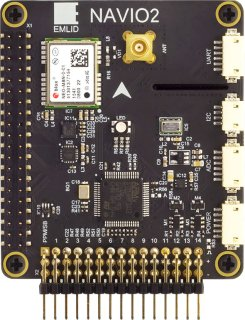
\includegraphics[width=0.4\linewidth, height=0.25\textheight]{Imagenes/navio22}
			\caption{Navio2}
			\label{fig:navio2}
		\end{figure}
		
		Dentro del conjunto de sensores que contiene esta placa tenemos:
		
	\subsubsection{IMU}
		Unidad de Medici�n Inercial (o por sus siglas en ingl�s \textit{Inertial Measurement Unit}) es el componente principal de los sistemas de navegaci�n. Son un conjunto de dispositivos electr�nicos, generalmente, una combinaci�n de aceler�metros, magnet�metros y giroscopios que miden e informan caracter�sticas del movimiento del veh�culo como pueden ser velocidad, fuerzas magn�ticas y orientaci�n. Como es un aspecto importante en este tipo de sistemas la precisi�n, la placa controladora Navio2 contiene dos de estas unidades con el fin de proporcionar y corroborar su informaci�n mediante dos fuentes de referencia distintas. Estas dos unidades son:
		
		\begin{enumerate}
			\item MPU9250 9DOF.
			\item LSM9DS1 9DOF.
			
		\end{enumerate}

	\subsubsection{GNSS}
		Obtener la posici�n del veh�culo mientras este se encuentra en movimiento es un aspecto sumamente necesario, m�s cuando la visibilidad del ambiente dificulta hacerlo, es por eso que el GNSS (\textit{Global Navigation Satellite System}) proporciona un posicionamiento geoespacial con cobertura global mediante un conjunto de tecnolog�as de sistemas de navegaci�n por sat�lite. Las tecnolog�as utilizadas en el m�dulo U-blox M8N de esta placa son:
		
		\begin{enumerate}
			\item Glonass.
			\item GPS.
			\item Beidou.
		\end{enumerate}


	\subsubsection{Entrada/Salida RC (Radio Control)} \label{sec:ioRC}
		La placa Navio2 tiene una entrada habilitada para recibir informaci�n proveniente del emisor mediante un radio control, aceptando se�ales por los protocolos de comunicaci�n PPM (Modulaci�n por Posici�n de Pulso) y SBUS �nicamente.
		

	\subsubsection{Bar�metro}
		El bar�metro tiene sus usos provenientes de la meteorolog�a para poder predecir el tiempo entre otras cosas, pero en este caso la placa controladora utiliza un bar�metro MS5611 de alta precisi�n (con 10cm de resoluci�n ) para poder estimar la altura en el cual se encuentra el dispositivo. 

	\subsubsection{Interfaces}
		\begin{itemize}
			\item Entrada UART (\textit{Universal Asynchronous Receiver-Transmitter})
			\item Bus de serie de datos $I^{2}C$ de sus siglas en ingl�s (Inter-Integrated Circuit)
			\item Conversor Anal�gico/Digital ADC
			\item Y por �ltimo. 14 salidas para servomotores mediante el protocolo PWM (Modulaci�n por Ancho de Pulso)
		\end{itemize}


	\subsection{Arduino UNO}
		El Arduino UNO es una plataforma computacional f�sica open-source basada en una simple tarjeta de I/O y un entorno de desarrollo que implementa el lenguaje Processing/Wiring. A diferencia de la Raspberry Pi 3, este est� fabricado para realizar tareas m�s sencillas, ya que su poder de procesamiento y memoria son limitados.
		\begin{itemize}
			\item Microcontrolador ATmega328.
			\item 14 pines digitales de I/O (6 salidas PWM).
			\item 6 entradas an�logas.
			\item 32KB de memoria Flash.
			\item Reloj de 16MHz de velocidad.	
		\end{itemize}
		\begin{figure}[h!]
			\centering
			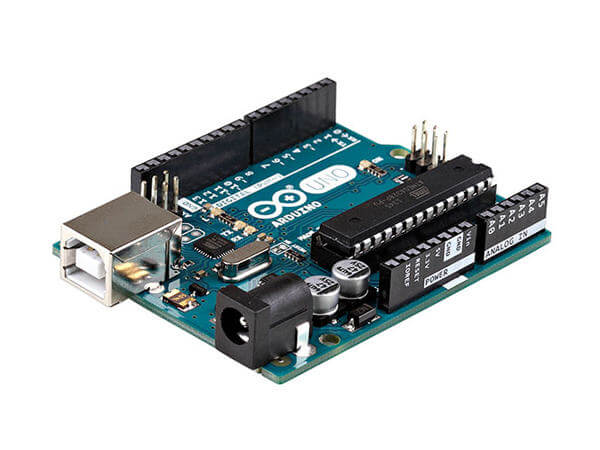
\includegraphics[width=0.5\linewidth, height=0.2\textheight]{Imagenes/arduinouno}
			\caption{Placa Arduino UNO}
			\label{fig:arduinouno}
		\end{figure}
		

	\subsection{Radio Control}
		Este control permite gobernar al veh�culo a distancia de manera inal�mbrica mediante se�ales de radio.
		\begin{figure}[h]
			\centering
			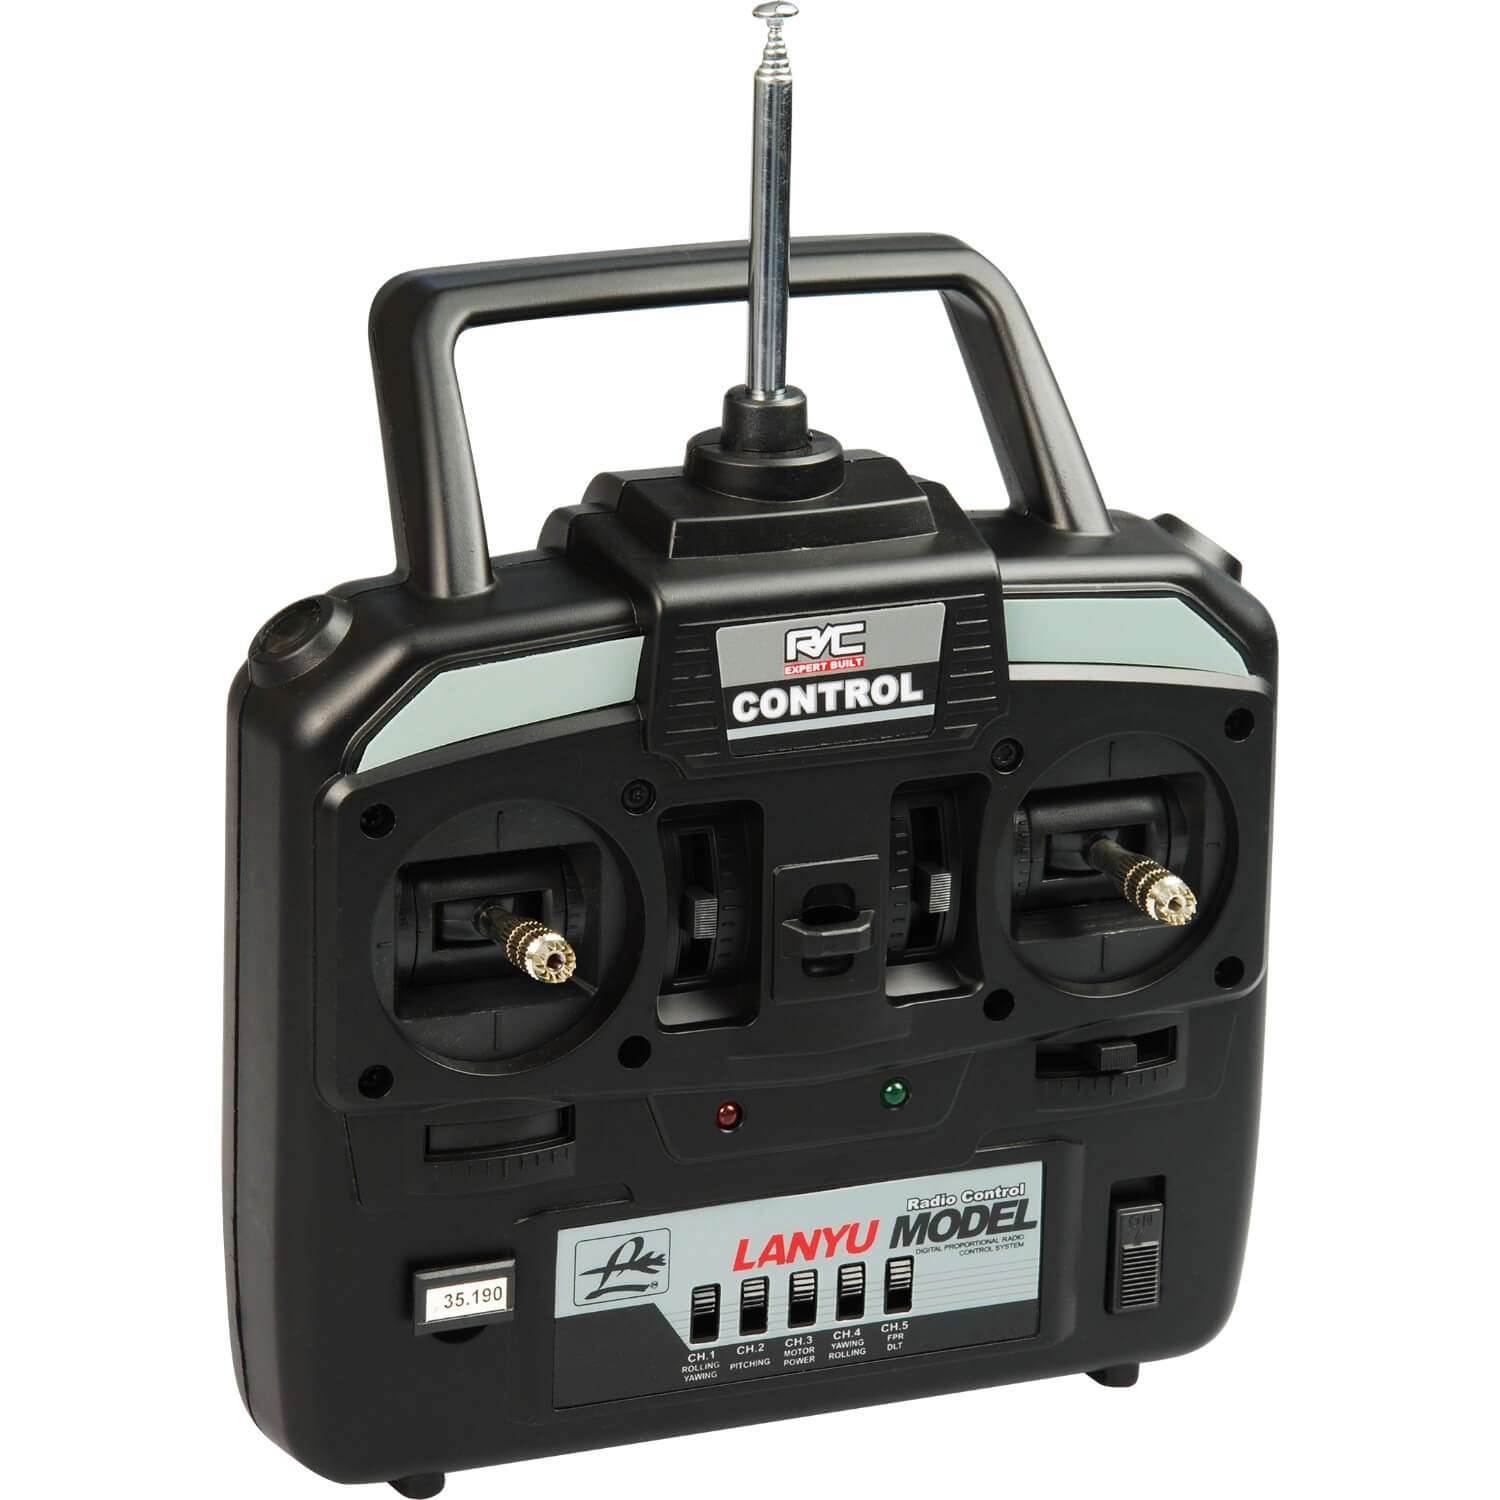
\includegraphics[width=0.4\linewidth, height=0.2\textheight]{Imagenes/RCcontrol}
			\caption{Comando Radio Control}
			\label{fig:rccontrol}
		\end{figure}



	\subsection{Joystick}	

		Una palanca de mando o com�nmente conocido como \textit{Joystick}  es un dispositivo que por lo general contiene 2 palancas con dos ejes cada uno, donde es posible representar la posici�n de un punto seg�n la posici�n f�sica de este y un conjunto de botones que al ser presionados y seg�n el software intermediario puede codificarse ciertas acciones. Este puede estar conectado mediante un cable USB o de manera inal�mbrica. En nuestro caso, utilizaremos un joystick con conexi�n USB ya que necesitamos que el env�o de informaci�n sea confiable.

	\subsection{Router}
	
		Un router es un dispositivo de hardware que permite la interconexi�n de ordenadores en red. El router o enrutador es un dispositivo que opera en capa de nivel de 3. As�, permite que varias redes u ordenadores se conecten entre s� y, por ejemplo, compartan una misma conexi�n de Internet. 
		\par Este dispositivo es usado para el desarrollo del proyecto ya que en el momento de las pruebas no se tienen a disposici�n los m�dulos de comunicaci�n verdaderos, estos m�dulos permiten una mayor distancia de cobertura y funciona exclusivamente para una conexi�n, lo que logra una mayor confiabilidad a la misma que comparando con el router que debe gestionar varias conexiones a la vez y la informaci�n enviada no est� asegurada. Por tal motivo de ausencia de estos m�dulos se recurre a utilizar como medio de comunicaci�n provisoria la tecnolog�a wifi del router, ya que �nicamente se pretende realizar pruebas en un �mbito controlado y de poca distancia.
	

	\subsection{M�dulos XBee}
	
		Los m�dulos XBee \footnote{P�gina web de XBee  https://www.digi.com/xbee} son soluciones integradas que brindan un medio inal�mbrico para la interconexi�n y comunicaci�n entre dispositivos. Estos m�dulos utilizan el protocolo de red llamado IEEE 802.15.4 para crear redes FAST POINT-TO-MULTIPOINT (punto a multipunto); o para redes PEER-TO-PEER (punto a punto). Est�n dise�ados para aplicaciones que requieren de un alto tr�fico de datos, baja latencia y una sincronizaci�n de comunicaci�n predecible.
	
		\begin{figure}[h!]
			\centering
			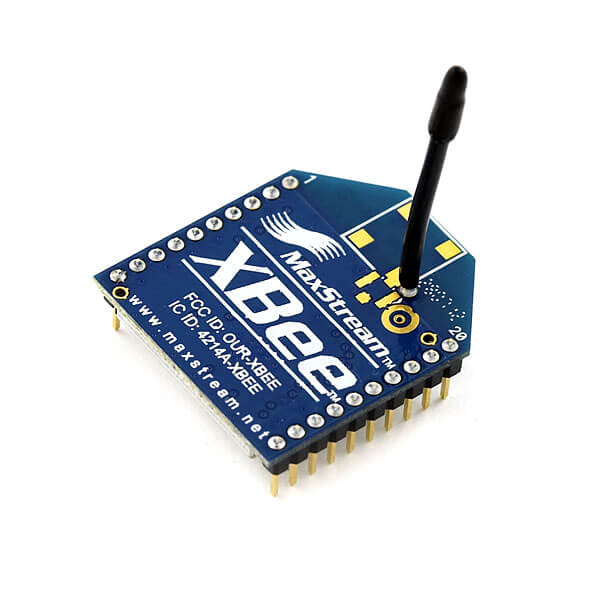
\includegraphics[width=0.4\linewidth, height=0.25\textheight]{Imagenes/xbee}
			\caption{M�dulo de comunicaci�n XBee}
			\label{fig:xbee}
		\end{figure}


	\subsection{Bater�a LiPo}
	
		La bater�a LiPo (Litio y Pol�mero) son bater�as recargables, compuestas generalmente de varias c�lulas conectadas en paralelo para aumentar la capacidad de la corriente de descarga. Esta contiene un voltaje de 12v con 2200 mA, suministrando dicha energ�a a los motores y adem�s a la Raspberry Pi con 5V.
		\begin{figure}[h!]
			\centering
			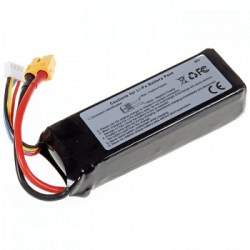
\includegraphics[width=0.2\linewidth, height=0.25\textheight]{Imagenes/bateria}
			\caption{Bater�a LiPo}
			\label{fig:bateria}
		\end{figure}
	


\section{Procedimiento}

	\subsection{Armado del cuerpo}
		Una vez ya descripto el hardware adquirido para el desarrollo de esta etapa,  estamos habilitados para iniciar el proceso del armado del veh�culo. En primera instancia se comienza con el cuerpo del cuadric�ptero, esta actividad  es realizada en base a las instrucciones que nos proporciona el vendedor \textit{ValueHobby} \footnote{http://www.valuehobby.com/media/wysiwyg/upload/Manual/bumblebee-manual.pdf} obteniendo el cuerpo armado como se puede observar en la Figura \ref{fig:armado}. Como medida de seguridad antes de realizar las pruebas se han extra�do las h�lices. Pero al momento se ser instaladas con el prop�sito de que el cuadric�ptero no se tumbe con respecto a su eje de orientaci�n cuando este se encuentre en el aire se deben colocar las h�lices pares de tal manera que su propulsi�n al momento de girar sea en sentido contra-horario y las h�lices impares deben estar colocadas en sentido horario tal como se ven en la Figura \ref{fig:esquemacuadricoptero} . 
		
		\begin{figure}[h!]
			\centering
			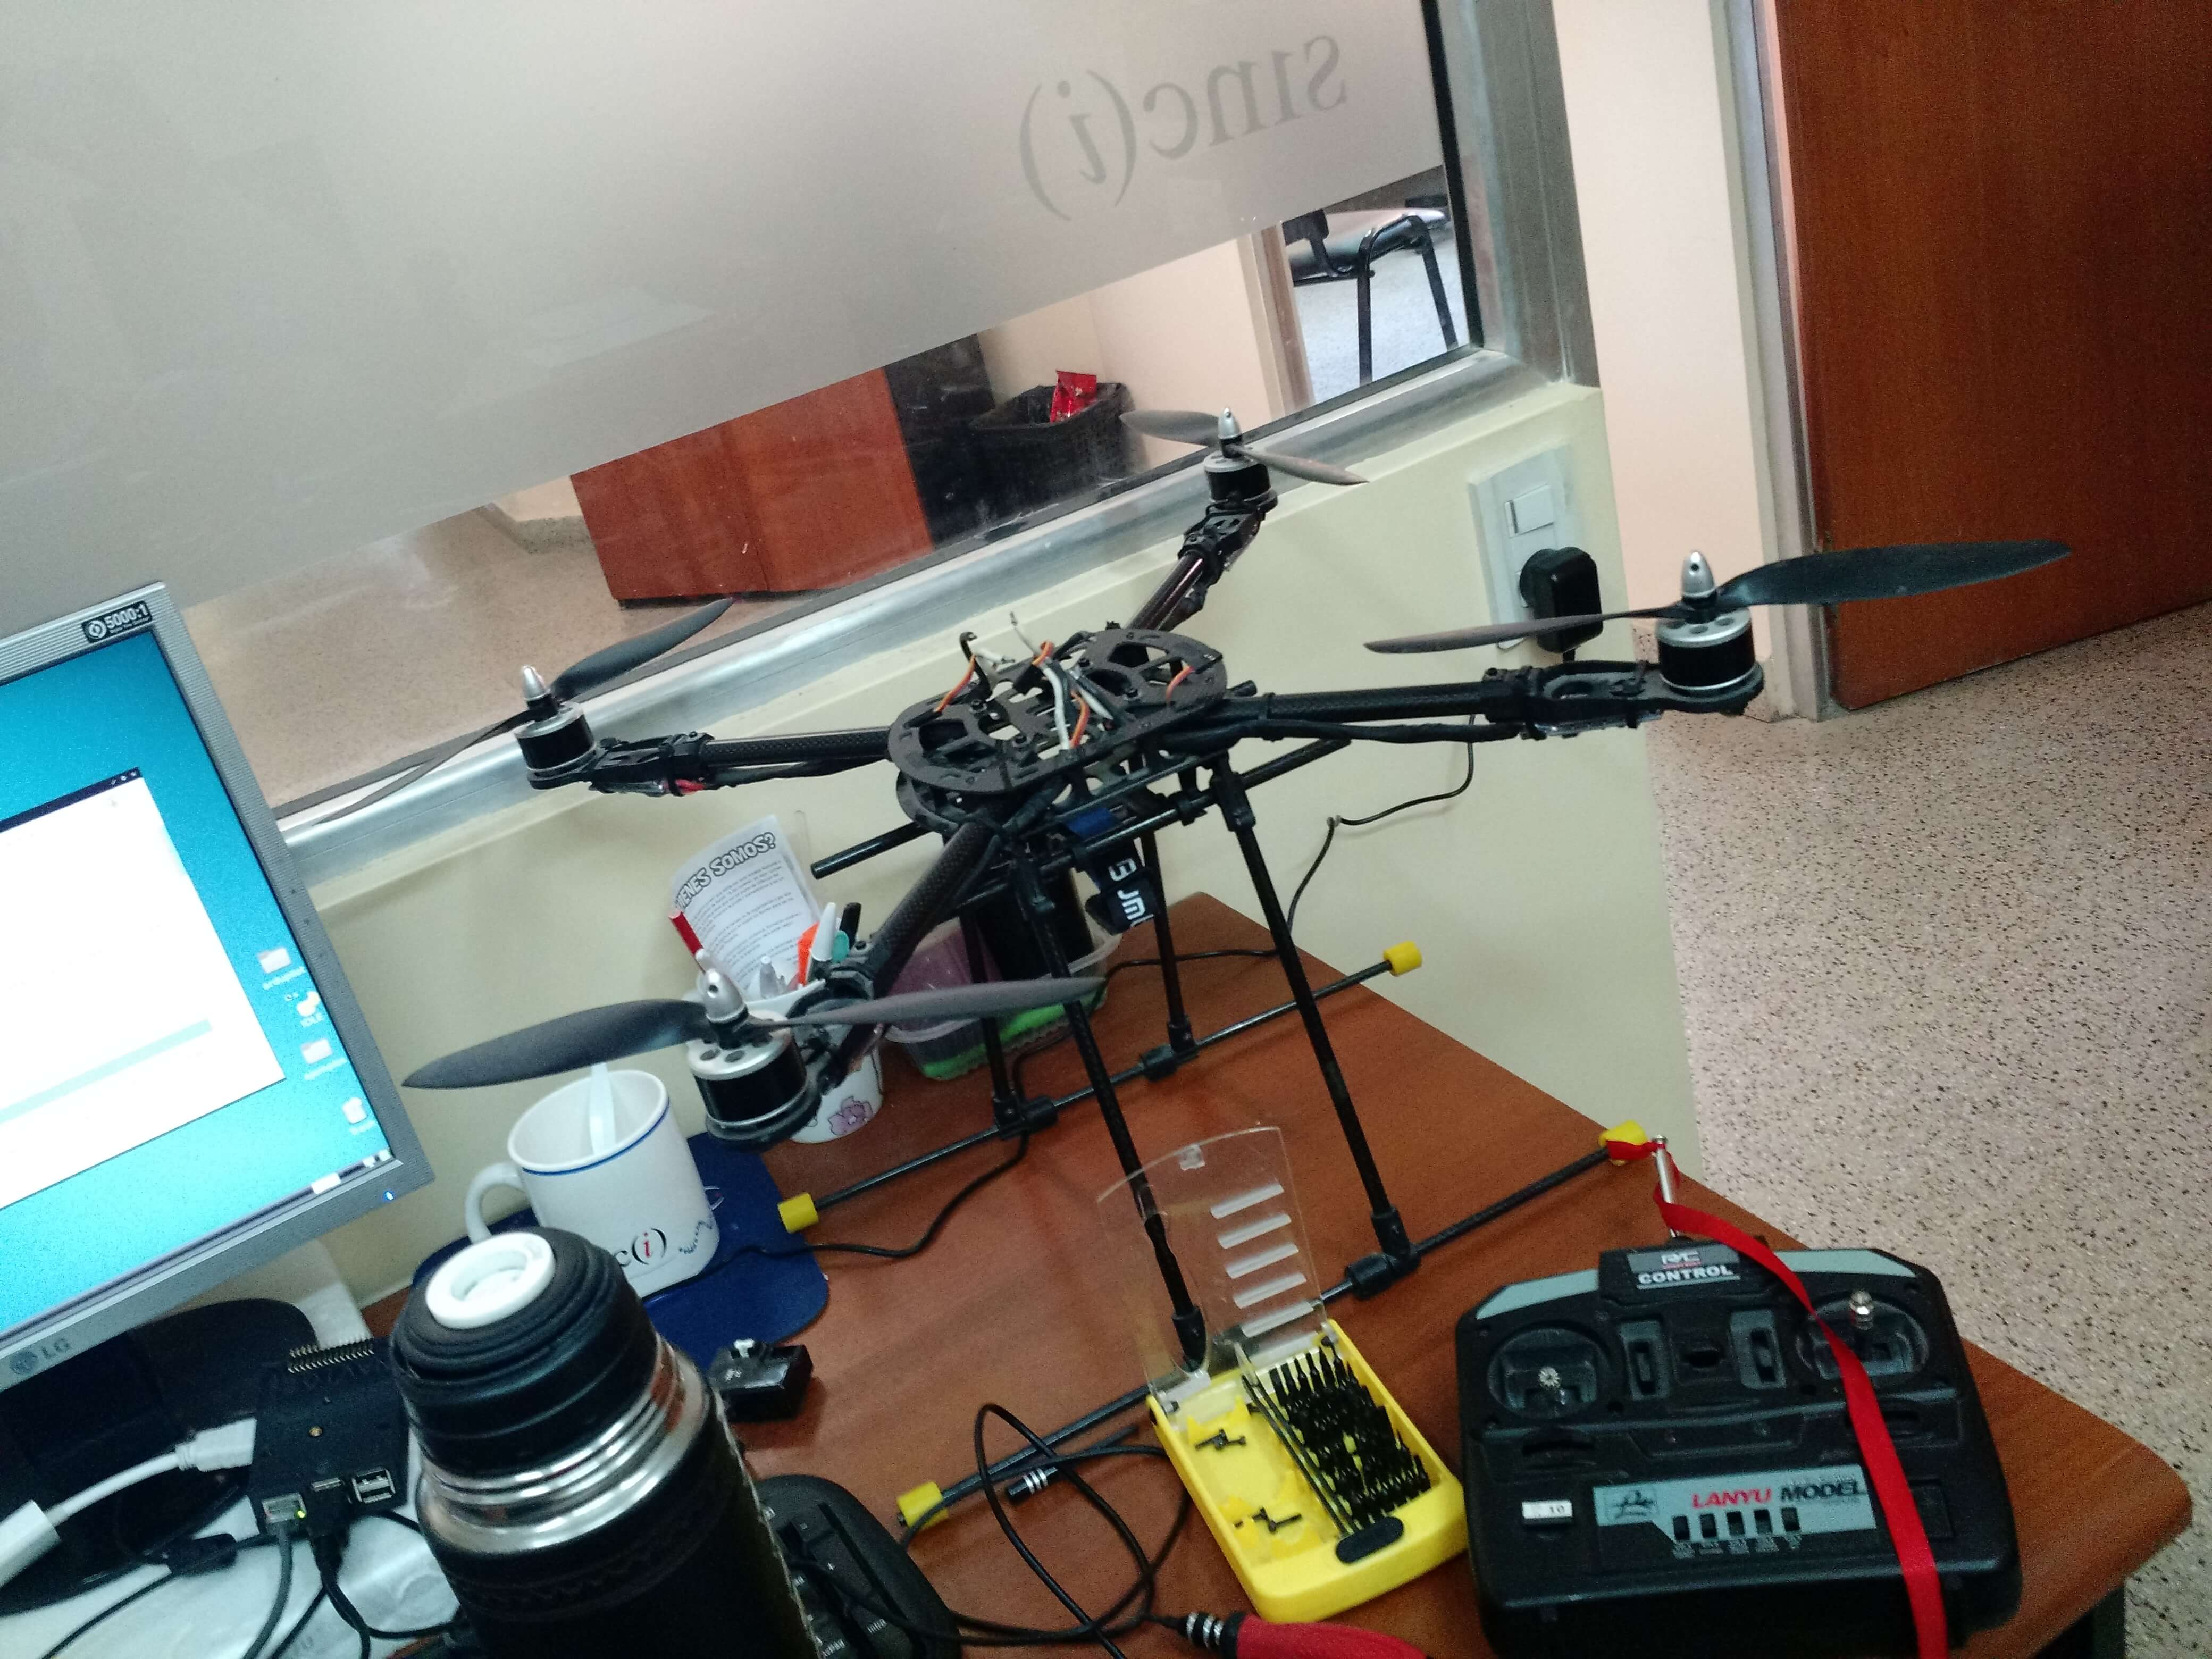
\includegraphics[width=0.6\linewidth, height=0.3\textheight]{Imagenes/fotos/Armado}
			\caption{Cuerpo de cuadric�ptero armado}
			\label{fig:armado}
		\end{figure}
		
		\begin{figure}[h!]
			\centering
			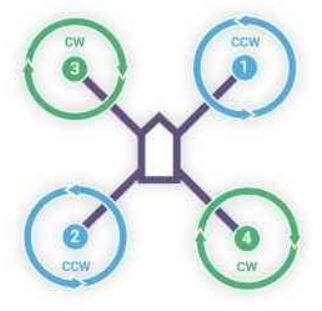
\includegraphics[width=0.3\linewidth, height=0.2\textheight]{Imagenes/esquemacuadricoptero}
			\caption{Esquema de instalaci�n de h�lices.}
			\label{fig:esquemacuadricoptero}
		\end{figure}

	\subsection{Armado y configuraci�n del piloto}
		En esta secci�n se describe el armado del piloto del cuadric�ptero, este va a ser el encargado en gestionar todos los sensores, enviar se�ales a los motores y administrar la informaci�n generada por estos sensores con el fin de ser enviadas a una maquina cliente y que este las pueda interpretar, entre otras cosas.
		
		
		\par Para comenzar con el armado debemos instalar la placa Navio2 sobre la Raspberry Pi 3, proporcionando as� los sensores indispensables para el control, monitoreo y vuelo del veh�culo ya que el ordenador de placa reducida Raspberry Pi no cuenta con estos sensores de forma nativa. Por lo tanto, se procede a conectar los 40 pines GPIO sobre la placa Navio2, como se muestra en la Figura \ref{fig:navio2-mount}
		
		
		\begin{figure}[h!]
			\centering
			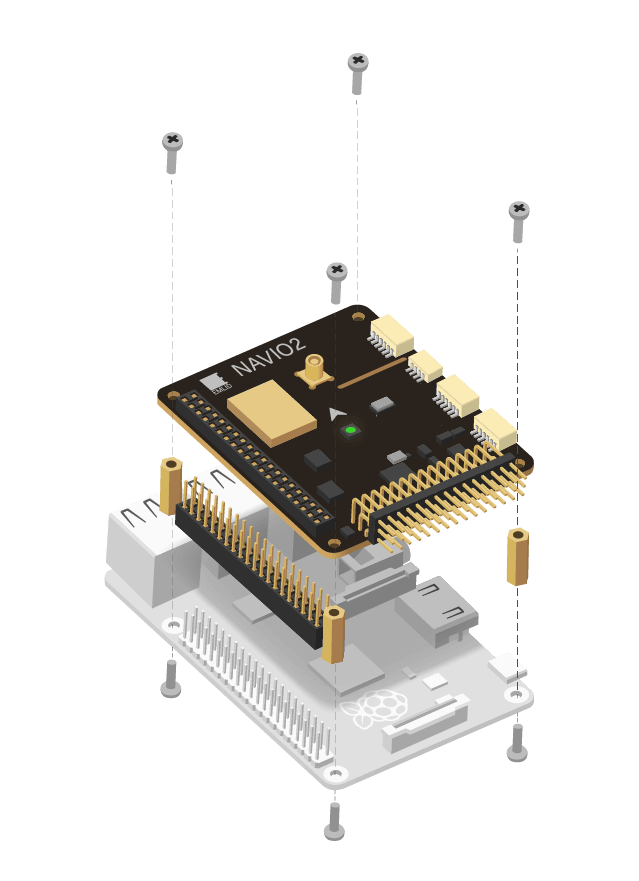
\includegraphics[width=0.4\linewidth, height=0.25\textheight]{Imagenes/navio2-mount}
			\caption{Conexi�n entre Raspberry Pi 3 y placa Navio2.}
			\label{fig:navio2-mount}
		\end{figure}
		
		Luego se procede a conectar la antena GNSS sobre la placa Navio2. Una vez ya conectado se debe verificar su correcto funcionamiento de todos los sensores presentes, para eso debemos tener un software que gestione eficazmente todo el hardware y sea el intermediario entre estos dispositivos electr�nicos y el usuario, adem�s de proporcionar servicios de utilidad para el mismo, en otras palabras, un sistema operativo (SO). Antes de instalar cualquier sistema operativo hay que tener en cuenta que  estamos en presencia de un ordenador de placa reducida, es decir, el hardware de los componentes del mismo como memoria, procesador, puertos de entrada y salida, etc�tera no son los mismos a los ordenadores comerciales que vemos com�nmente; por poner un ejemplo, el procesador que contiene la Raspberry es un ARM1176JZF-S, con esto queremos decir que el CPU en si mismo esta fabricado bajo una arquitectura con un conjunto reducido de instrucciones (o por su siglas en ingles \textit{RISC - Reduced instruction set computing}) en comparaci�n a un CPU que son utilizados normalmente en un ordenador hogare�o. Por tal motivo, es necesario de un SO que se adapte a estas caracter�sticas; afortunadamente existen varias organizaciones o empresas que desarrollan y distribuyen este tipo de producto, por ejemplo, \textit{Canonical Ltd} y \textit{Microsoft} han adaptado sus sistemas operativos para este tipo de ordenadores. En nuestro caso utilizaremos un SO proporcionado por la empresa \textit{Emlid} basado en una distribuci�n de Linux llamada \textit{Raspbian} (acr�nimo entre Raspberry Pi y Debian) donde ya viene preinstalado las herramientas necesarias.
		\par Una vez seleccionado el SO a instalar, se procede a descargar la imagen y grabarla en una tarjeta SD, una vez realizado este paso se carga la tarjeta SD en la ranura disponible en la Raspberry Pi, se enchufa un teclado, mouse y un conector HDMI que se encuentra conectado a un monitor, y por �ltimo se procede a encender el dispositivo  mostr�ndonos la siguiente imagen: 
		
		
		\begin{figure}[h!]
			\centering
			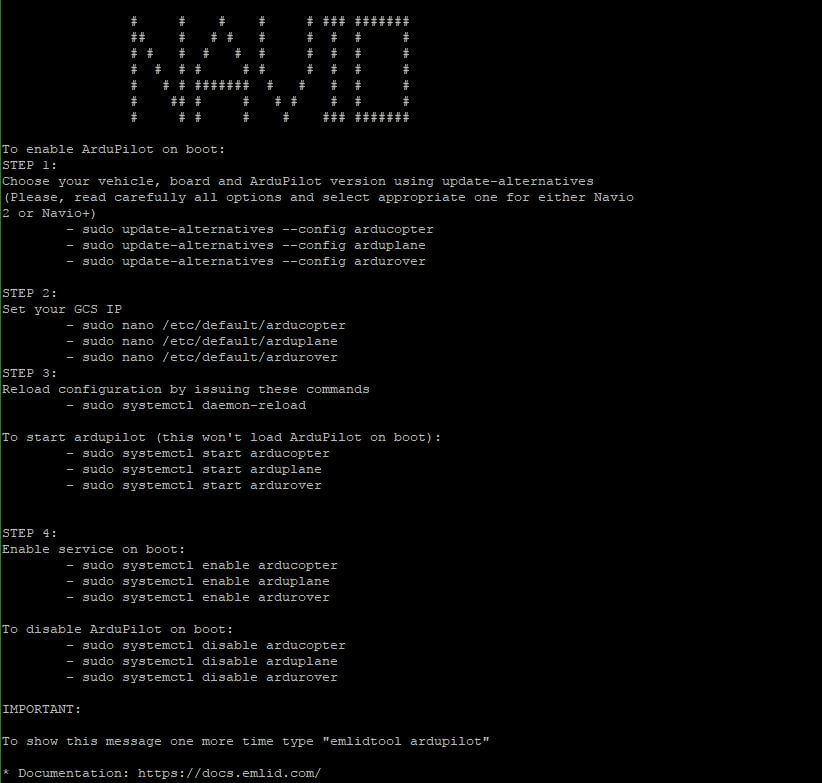
\includegraphics[width=0.8\linewidth, height=0.37\textheight]{Imagenes/pantallaInicio}
			\caption{Pantalla de bienvenida luego de instalar el SO}
			\label{fig:pantallainicio}
		\end{figure}
		
		Como se puede observar en la imagen \ref{fig:pantallainicio} la pantalla de bienvenida nos muestra los siguientes pasos que hay que seguir para configurar nuestro piloto.
		\begin{itemize}
			\item \textbf{Paso 1:} Se selecciona el tipo de veh�culo que se va a manejar, utilizando el comando \textit{update-alternatives}. Esta funci�n se encarga de seleccionar como predeterminada la opci�n ingresada dentro de otras alternativas, es decir, 
			Es posible que tenga en el sistema varios programas instalados a la vez  que  realizan  la
			misma  funci�n. Por ejemplo, muchos sistemas tienen varios editores de texto instalados al
			mismo tiempo, lo que deja la elecci�n de  qu�  editor  de  texto  utilizar  en  manos  del
			usuario,  si  �ste lo desea, pero hace dif�cil que un programa elija la opci�n correcta si
			el usuario no ha definido ninguna preferencia. En nuestro caso es el tipo de autopiloto como puede ser arducopter, arduplaner y ardurover. Como estamos por utilizar un cuadric�ptero ingresamos:
			
			\begin{listing}[style=consola, numbers=none]
				> sudo update-alternatives --config arducopter
			\end{listing}
				
				
				
				\item \textbf{Paso 2:} Se debe ingresar dentro del archivo /etc/default/arducopter el IP perteneciente al GCS (\textit{Ground Control Station}), es decir, este archivo contiene la direcci�n IP del ordenador que enviar� y recibir� informaci�n del veh�culo. Adem�s, brinda la opci�n de seleccionar la interfaz por el que se realizar� la comunicaci�n. En nuestro caso lo haremos realizaremos mediante tecnolog�a Wifi y utilizando el protocolo UDP \footnote{Es posible tambi�n utilizar el protocolo TCP, pero la raz�n por la cual se este m�todo es porque es un protocolo no orientado a la conexi�n, por lo tanto como estaremos realizando maniobras que son ejecutadas por el veh�culo en tiempo real necesitamos la menor latencia posible y no estar esperando paquetes de confirmaci�n todo el tiempo}. 
				
				\item \textbf{Paso 3:} Una vez ya seleccionado el tipo de veh�culo a utilizar e ingresado el IP de nuestro GCS se debe iniciar los servicios y procesos proporcionados por arducopter (ya que este se encargar� de administrar las funcionalidades pertinentes), para eso se utiliza el gestor del sistema y servicios \textbf{systemd} de Linux con el objetivo de iniciar un conjunto nuevo de procesos y servicios encapsulados en Arducopter, para eso utilizamos los siguiente comandos :
				
				\begin{listing}[style=consola, numbers=none]
				> sudo systemctl daemon-reload
				> sudo systemctl start arducopter 
				\end{listing}
				
				
				
				
				\item \textbf{Paso 4:} Por �ltimo es deseable que los servicios proporcionados por Arducopter se inicien cada vez que el veh�culo se encienda, por tal motivo se ingresa el �tlimo comando :
				
				\begin{listing}[style=consola, numbers=none]
				> sudo systemctl enable arducopter 
				\end{listing}
			
			
			
		\end{itemize}

	\subsection{Configuraci�n para el acceso a la red}

		\par Entre las opciones de conexi�n a la red que dispone la Raspberry Pi 3, podemos identificar que el mismo tiene una entrada Ethernet como tambi�n un m�dulo interno Wi-Fi, por lo tanto es necesario configurar dichas interfaces para poder conectarnos mediante un cable UTP con un conector RJ45, como tambi�n por tecnolog�a \textit{Wireles}. Por lo que dentro del sistema operativo del veh�culo y sobre la consola se ingresa el siguiente comando 
		\begin{listing}[style=consola, numbers=none]
			> sudo ifconfig
		\end{listing}
		Con este comando podemos verificar nombres de interfaces presentes y si se encuentran en actual funcionamiento. En caso de observar ning�n tipo de trafico por estas interfaces se procede a configurarlas, para esto se utiliza el mismo comando pero con la opci�n de activar la interfaz deseada, en nuestro caso queremos activar la interfaz del m�dulo interno de Wi-Fi, para eso ingresamos el siguiente comando 
		\begin{listing}[style=consola, numbers=none]
		> sudo ifconfig intwifi0 up
		\end{listing}
		Una vez ya activo podemos buscar las redes disponibles y que son captadas por el m�dulo, utilizando el siguiente comando 
		
		\begin{listing}[style=consola, numbers=none]
			> iwlist wlan0 scan
			\end{listing}
			Con este comando nos muestra mediante una lista las redes captadas por el m�dulo, una vez que hayamos encontrado la red de nuestro inter�s podemos conectarnos con el siguiente comando 
			
			\begin{listing}[style=consola, numbers=none]
			> iwconfig wlan0 essid "Nombre de Red" key "Contrasena"
		\end{listing}
		y finalmente procederemos a obtener nuestra IP y conectarnos con la siguiente funci�n :

		\begin{listing}[style=consola, numbers=none]
		> sudo dhclient wlan0
		\end{listing}
		
		En caso de querer almacenar esta red e indicarle al sistema operativo que es nuestra red por defecto podemos modificar el archivo wpa\_supplicant.conf ingresando el nombre de la red y su correspondiente clave.
		Por �ltimo, se reinicia y una vez iniciado el sistema se comprueba su conectividad realizando chequeo de conexi�n con alg�n tipo de p�gina en internet, por ejemplo, Google utilizando el siguiente comando 
		\begin{listing}[style=consola, numbers=none]
		> ping 8.8.8.8
		\end{listing}


	\subsection{Instalaci�n del firmware}

		\par Una vez ya comprobado la conectividad a la red y conFigurado el sistema operativo, es necesario instalar el \textit{firmware}  encargado de gestionar todos los sensores que se han incluido a la Raspberry mediante la placa Navio2, con el objetivo de poder administrar esta informaci�n y poder enviarla al \textit{GCS}. Para instalar el firmware se procede a descargarlo desde el mismo SO del veh�culo mediante el siguiente comando 
		
		
		\begin{listing}[style=consola, numbers=none]
			
			pi@navio: ~\$ wget http://firmware.eu.ardupilot.org/Copter/stable/navio2-quad/arducopter-quad
			pi@navio: ~\$ chmod +x arducopter-quad}
		
		\end{listing}
		
		Una vez descargado el firmware se desea que los servicios ya instalados de Arducopter utilicen dicho firmware actualizado, por lo tanto se procede a modificar el archivo /etc/systemd/system/ardupilot.service. Modificando la l�nea  
		
		\begin{listing}[style=consola, numbers=none]
		#ExecStart=/bin/sh -c "/home/pi/path/to/your/binary \$\{ARDUPILOT\_OPTS\}"
		\end{listing}
		por
		\begin{listing}[style=consola, numbers=none]
		#ExecStart=/bin/sh -c "/home/pi/arducopter-quad \$\{ARDUPILOT\_OPTS\}"}
		\end{listing}


	\subsection{Primeras pruebas}	\label{sec:primprue}
		Ya instalado el firmware correspondiente dentro de la Raspberry Pi estamos en condiciones de poder hacer nuestras primeras pruebas, para eso, dentro del mismo veh�culo se ejecutan programas proporcionados por ArduPilot para poder observar los datos generados por los sensores. En la misma carpeta de instalaci�n se encuentran programas de ejemplo para observar los datos provenientes de los sensores y al ejecutar dichos programas evidentemente la informaci�n mostrada es err�nea ya que estos sensores no se encuentran calibrados, por lo tanto, para realizar estas correcciones utilizamos las herramientas recomendadas y proporcionadas por la empresa ArduPilot como es el software \textbf{MavProxy} (Figura \ref{fig:mavproxy}), este software muestra a trav�s de una consola todos los datos obtenidos de los sensores, estado del veh�culo entre otras cosas, siendo lo m�s importante poder calibrar los sensores.
		\begin{figure}[h]
		\centering
		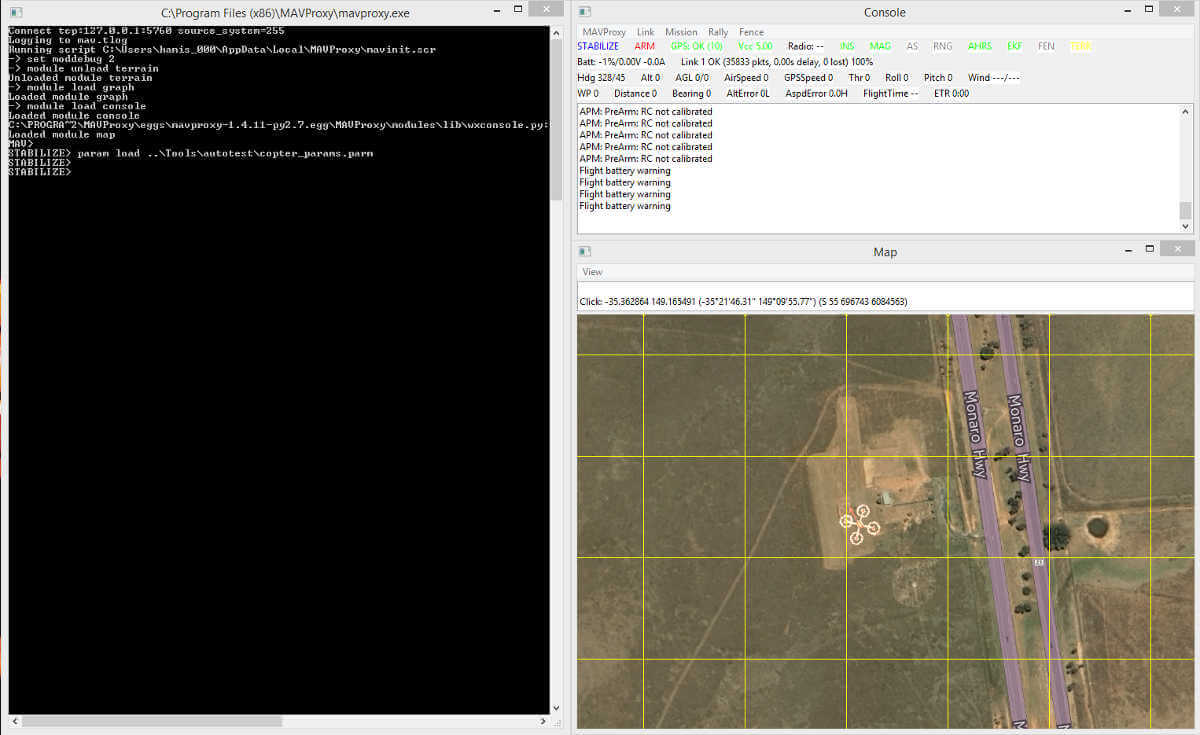
\includegraphics[width=0.8\linewidth, height=0.4\textheight]{Imagenes/mavproxy}
		\caption{Captura de pantalla del Software MavProxy}
		\label{fig:mavproxy}
		\end{figure} 
		As� que una vez iniciado el software se prueba la opci�n de calibrarlos. Al momento de iniciar el proceso de calibraci�n surge el inconveniente de no poder iniciarlo, ya que para realizar dicha acci�n es de suma importancia tener conectado el radio control al veh�culo. Esto genera un inconveniente al momento del desarrollo de esta fase ya que la compra de un radio control conllevar�a un tiempo extra en el cronograma del proyecto. Buscando alternativas en conjunto se descubre que es posible realizar la calibraci�n mediante un script que deb�amos codificar. Analizando esta propuesta se descubre que para generar dicho script es necesario de estudiar las librer�as involucradas lo que conlleva un tiempo considerado y �nicamente el objetivo de esta fase es realizar la comprobaci�n funcional de estos dispositivos. De esta manera se obtiene provisoriamente un radio control como se ilustra en la imagen \ref{fig:radiocontrol}
		
		\begin{figure}[h!]
		\centering
		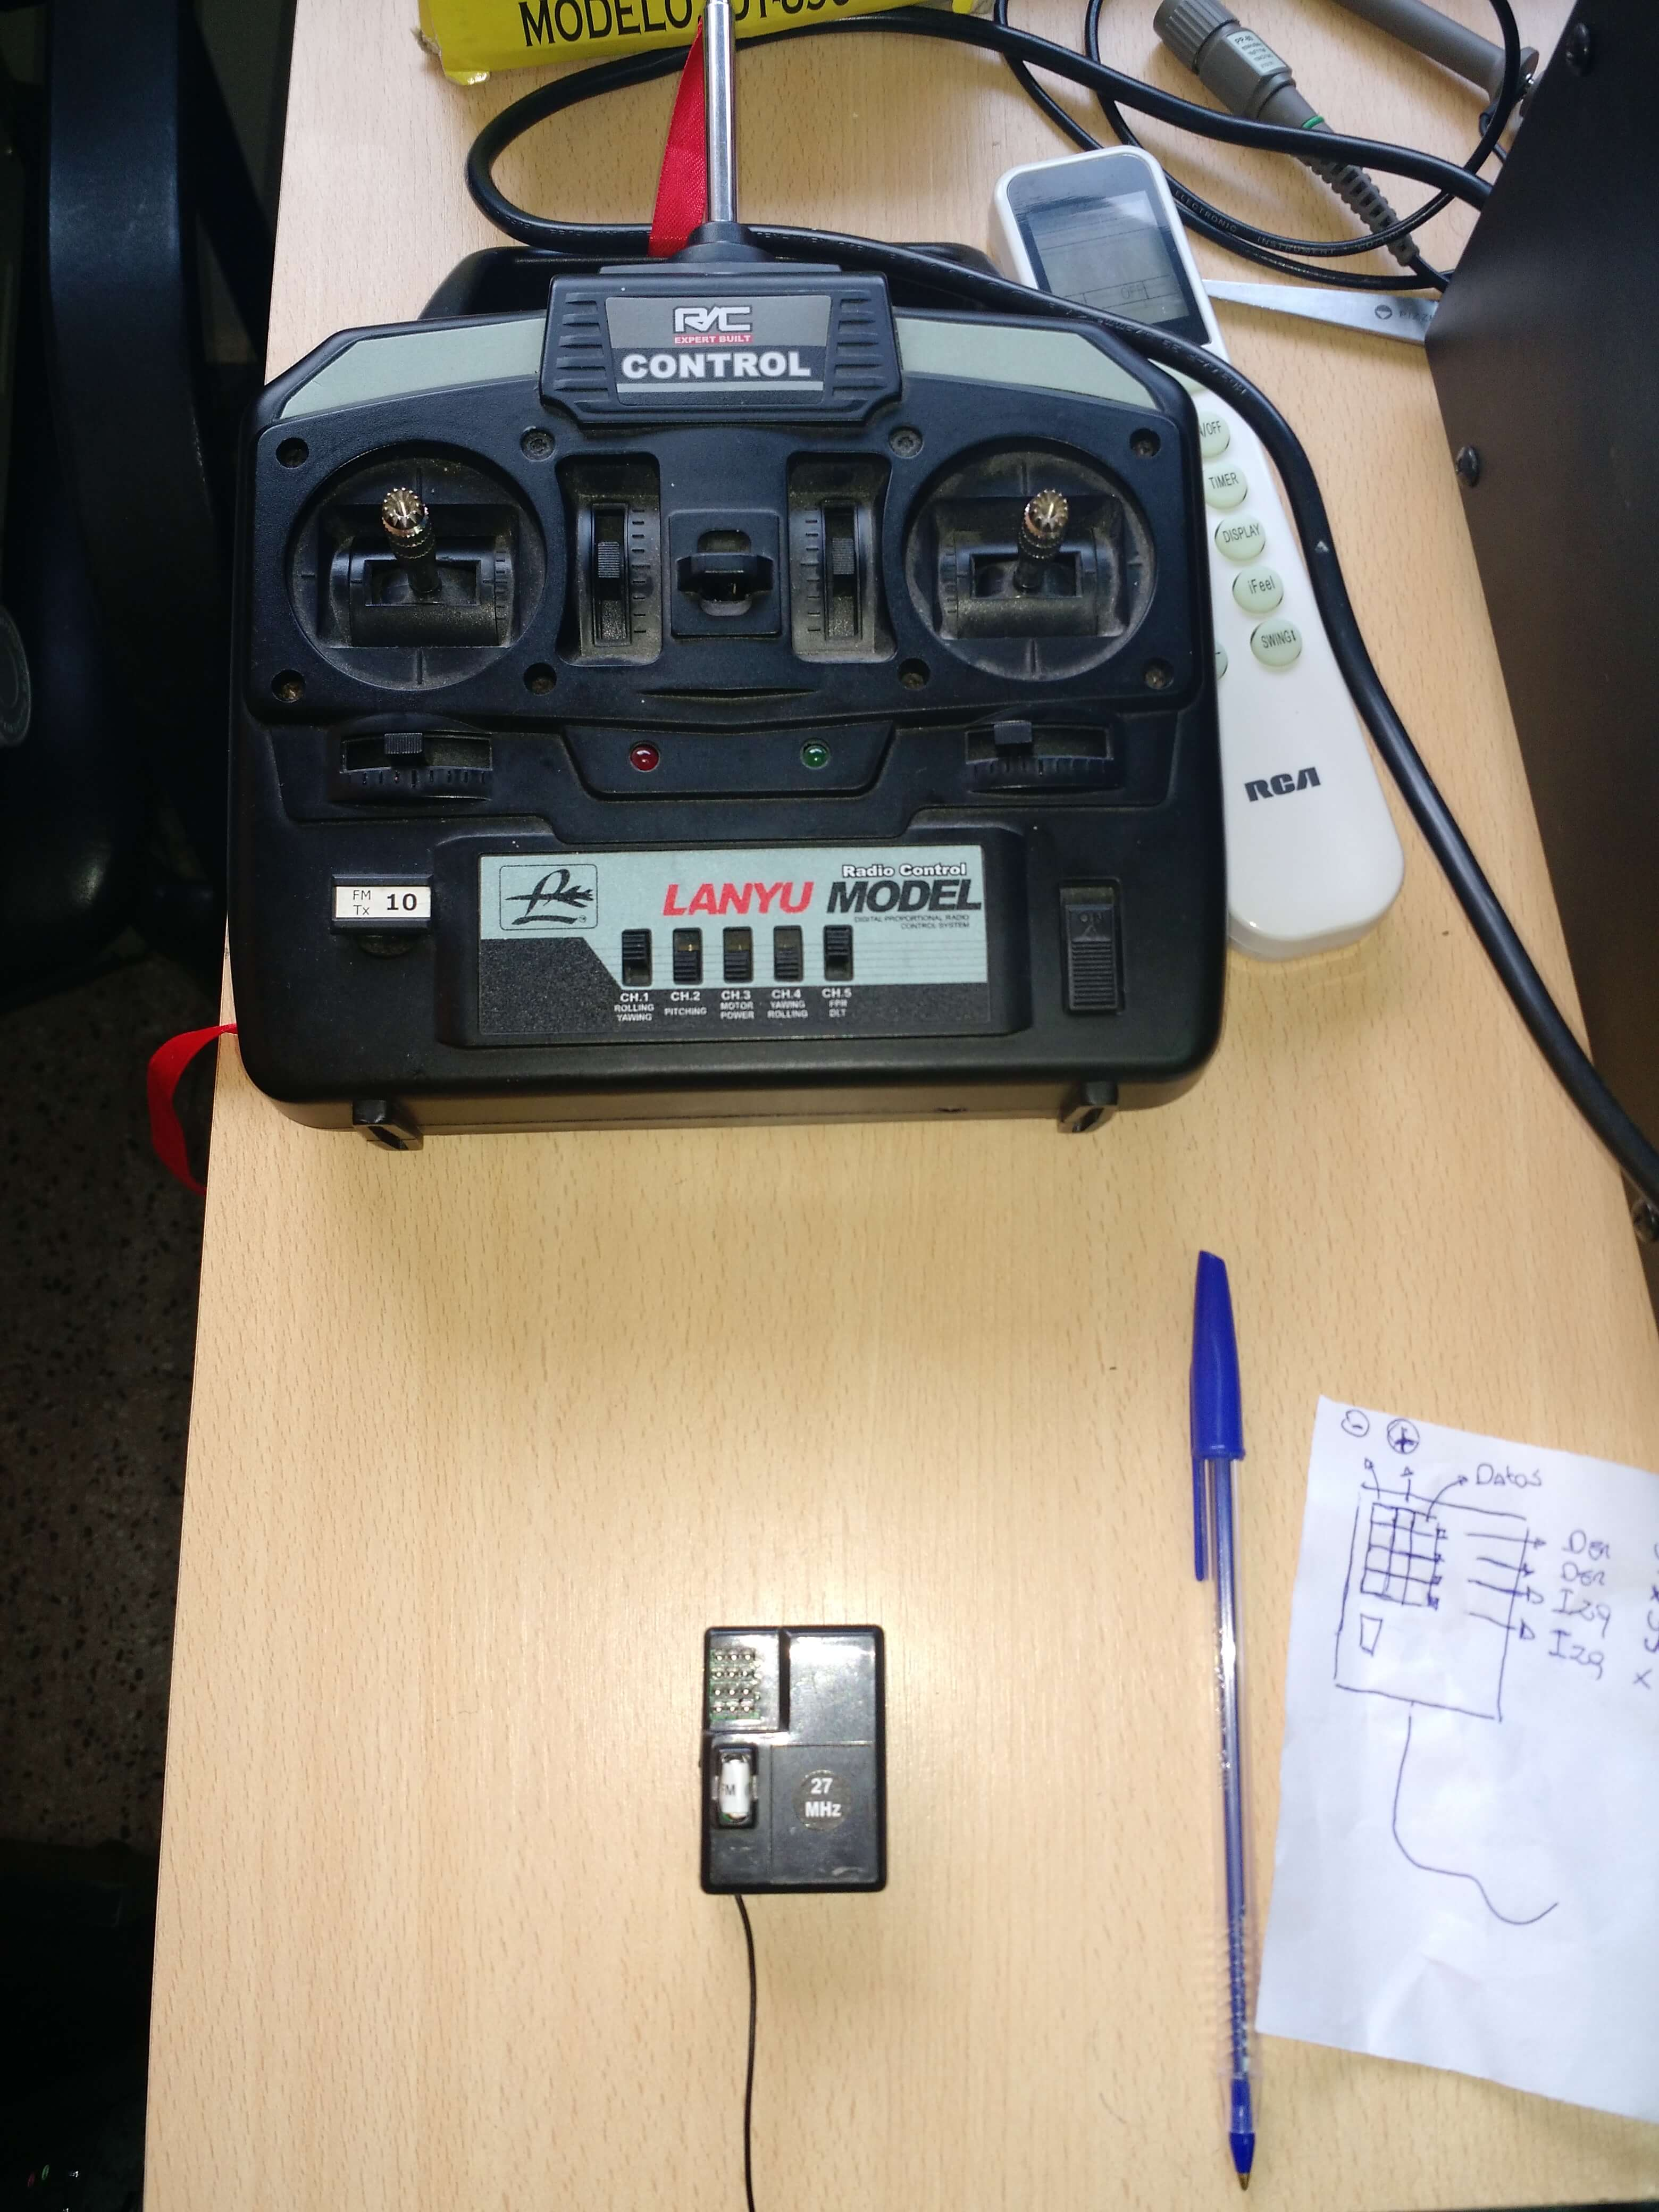
\includegraphics[width=0.5\linewidth, height=0.5\textheight]{Imagenes/fotos/rc_control_receptor}
		\caption{Radio Control LANYU model y su correspondiente receptor.}
		\label{fig:radiocontrol}
		\end{figure}
		
		Este radio control simplemente env�a las se�ales por 4 canales independientes, que son generados por sus dos palancas donde cada una contiene 2 ejes (\textit{eje x y eje y}), por lo tanto tendr�amos que la palanca 1 enviar� informaci�n del $eje_{p1} x$ y $eje_{p1} y$ y de la misma manera, la palanca 2 enviar� informaci�n de el $eje_{p2} x$ y $eje_{p2} y$ mediante la t�cnica de modulaci�n por ancho de pulso. Simplificando un poco, el receptor o (\textit{RX})  tendr� 4 cables con informaci�n de cada canal y que deber� conectarse al veh�culo, pero recordando la secci�n \ref{sec:ioRC} el veh�culo solo dispone de una entrada compatible con PPM o SBUS. Por lo que aqu� surge otro problema, debemos encontrar la forma de poder convertir las se�ales del radio control que se encontraban en PWM y pasarlas a PPM o SBUS para que el veh�culo pueda interpretar esta informaci�n. Para solucionar este problema se plantean 3 alternativas:
		
		\begin{enumerate}
		\item \textbf{Comprar un radio control con su respectivo receptor compatible con el veh�culo.}   
		\item \textbf{Realizar manualmente un conversor de PWM a PPM o SBUS con componentes electr�nicos desde cero. }   
		\item \textbf{Implementar el conversor sobre una placa Arduino UNO.}   
		\end{enumerate}
		
		Para estas propuestas se realiza el siguiente an�lisis:\newline
		\par \textbf{Propuesta 1: } La adquisici�n de un nuevo radio control m�s all� de sus futuros usos conllevar�a un elevado costo adicional para el proyecto ya que el mismo tiene un valor de \$8000 \footnote{Fecha consultada, septiembre del 2017}, adem�s atrasar�a el cronograma los d�as que se deban esperar el producto desde su ciudad de origen.
		
		\par \textbf{Propuesta 2: } Consiste en realizar la compra de los componentes electr�nicos de tipo CMOS CD4001 \footnote{http://www.alldatasheet.es/datasheet-pdf/pdf/26834/TI/CD4001.html} y 	CD40106 \footnote{http://www.alldatasheet.es/datasheet-pdf/pdf/26839/TI/CD40106.html} con un precio estimado de \$100. A pesar de su bajo costo de implementaci�n y siendo la mano de obra realizada por el profesor de la c�tedra Electr�nica Digital, es una tarea ajena al ejecutante del proyecto, por lo que no complementar�a los conocimientos del alumno.
		
		\par \textbf{Propuesta 3: } Esta propuesta consiste en implementar la funci�n de conversi�n de PWM a PPM o SBUS mediante un script que se implementar� sobra la placa Arduino, donde se conectar�n los cables provenientes del Rx a sus entradas y retornar� en una de sus salidas un �nico cable con la informaci�n codificada en PPM o SBUS como estaba especificado en el sitio web del fabricante. El precio estimado de la placa Arduino UNO es de \$200, pero existen versiones reducidas como el Arduino Nano que cuentan con un precio a la mitad del Arduino UNO. De manera conveniente se contaba con la adquisici�n de un Arduino UNO, por lo que no hacia falta realizar una compra. Adem�s, la implementaci�n de este algoritmo contribuye al crecimiento de las aptitudes del ejecutante del proyecto como estudiante de ingenier�a en inform�tica. 
		% TODO: Explicar codificaci�n del script	 
		Por lo que finalmente se decide realizar la propuesta 3. Una vez realizada se implementa sobre la placa Arduino UNO y se comprueban los resultados con un osciloscopio, d�ndonos un resultado favorable.




	\subsection{Conexi�n de componentes}
		
		Antes de comenzar a describir el proceso de cableado del veh�culo se comienza conectando el receptor del comando radio control con el Arduino UNO que va a ser el en cargado de recibir las se�ales PWM y convertirlas en SBUS moment�neamente para poder enviarlas a la Navio2. Hay que tener en cuenta que la ubicaci�n de los conectores y los pines del receptor llevan un orden en espec�fico. Por tal motivo, se investiga dicho orden, pero sin encontrar informaci�n relevante, hasta ubicar con un transmisor de la misma empresa y deducir las siguientes conexiones
		
		
		\begin{figure}[h!]
		\centering
		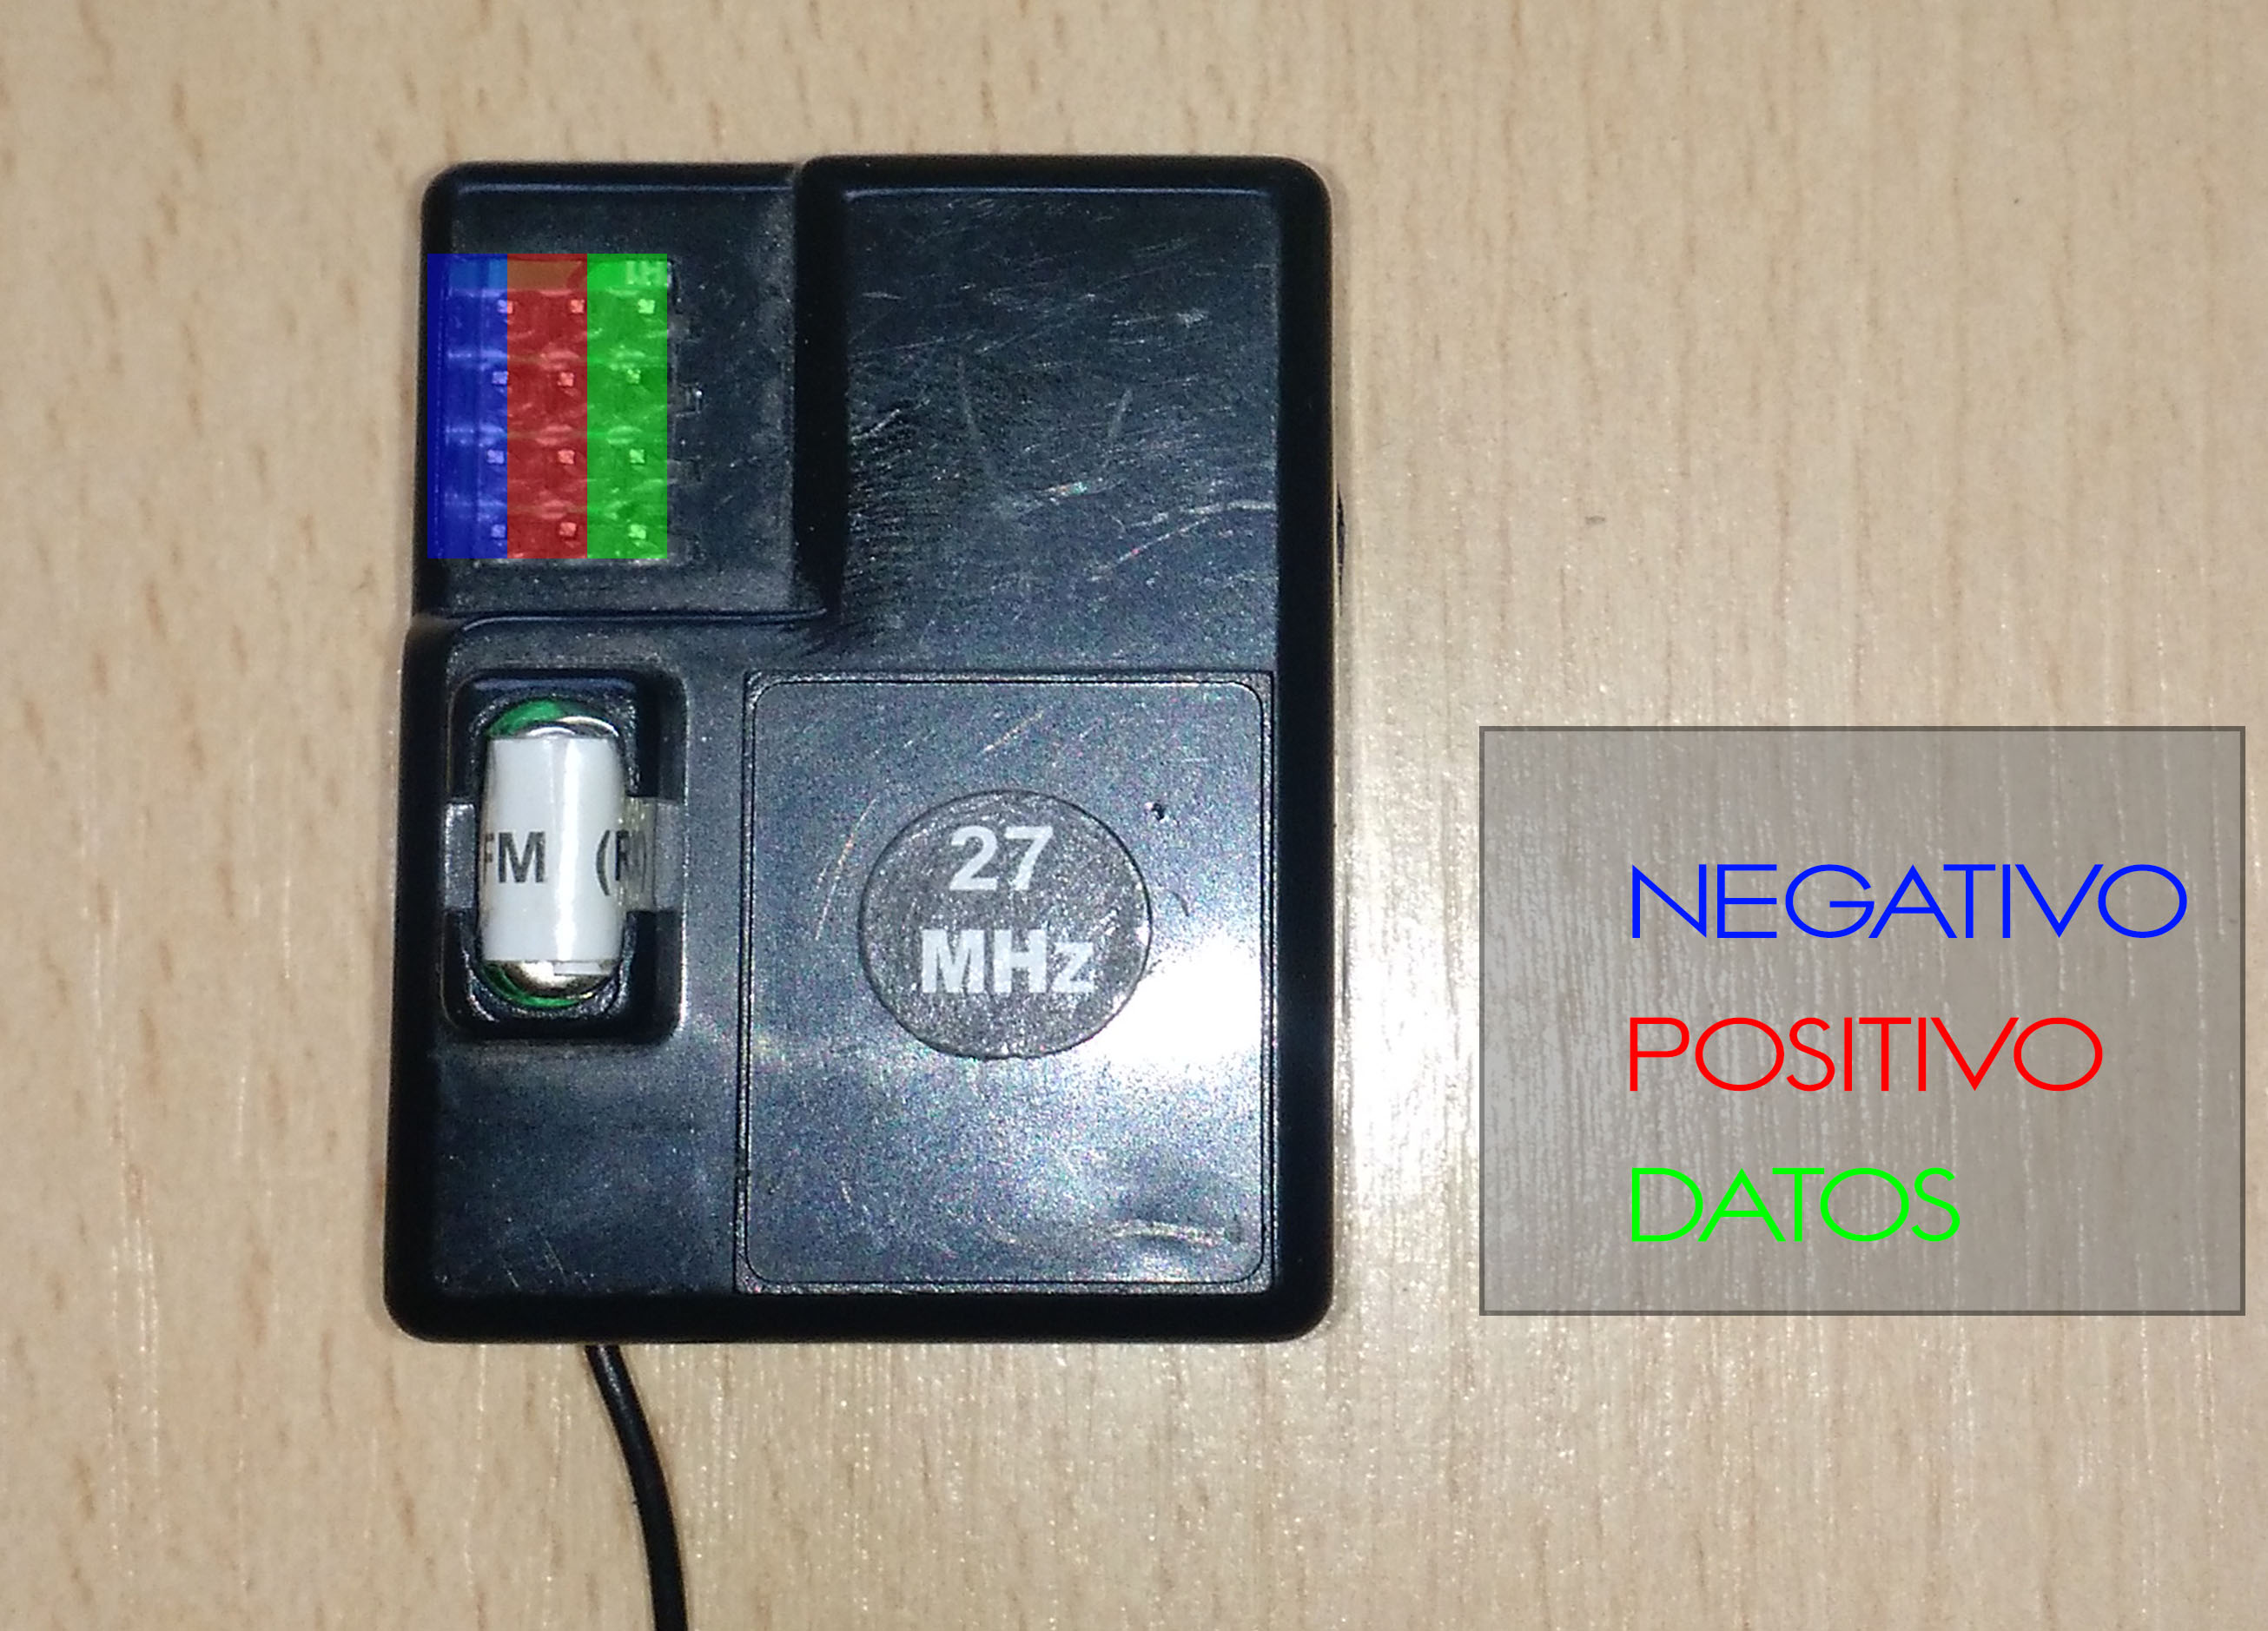
\includegraphics[width=0.5\linewidth, height=0.3\textheight]{Imagenes/fotos/Rxconexion}
		\caption{Ubicaci�n de conexiones en el Rx}
		\label{fig:RxConexiones}
		\end{figure}
		
		Como se puede observar en la Figura \ref{fig:RxConexiones} la columna izquierda de pines le pertenece a los negativos, la columna central a los positivos y la �ltima columna perteneciente a datos; esta es la de inter�s ya que por cada $conector_i$ estar�amos recibiendo se�al PWM del emisor correspondiente al $canal_i$, por lo que cada una son las entradas a nuestro Arduino UNO para poder realizar la codificaci�n. Antes de iniciar la conexi�n con el codificador se comprueban las se�ales mediante un osciloscopio. 
		\par Ya identificados los cables correspondientes a cada canal, se conectan los mismos a la placa Arduino UNO. Por �ltimo, se conecta la salida proporcionada por el codificador a la entrada del veh�culo, asegurando as� una se�al de tipo SBUS como lo indica su fabricante.
		
		\begin{figure}[h!]
		\centering
		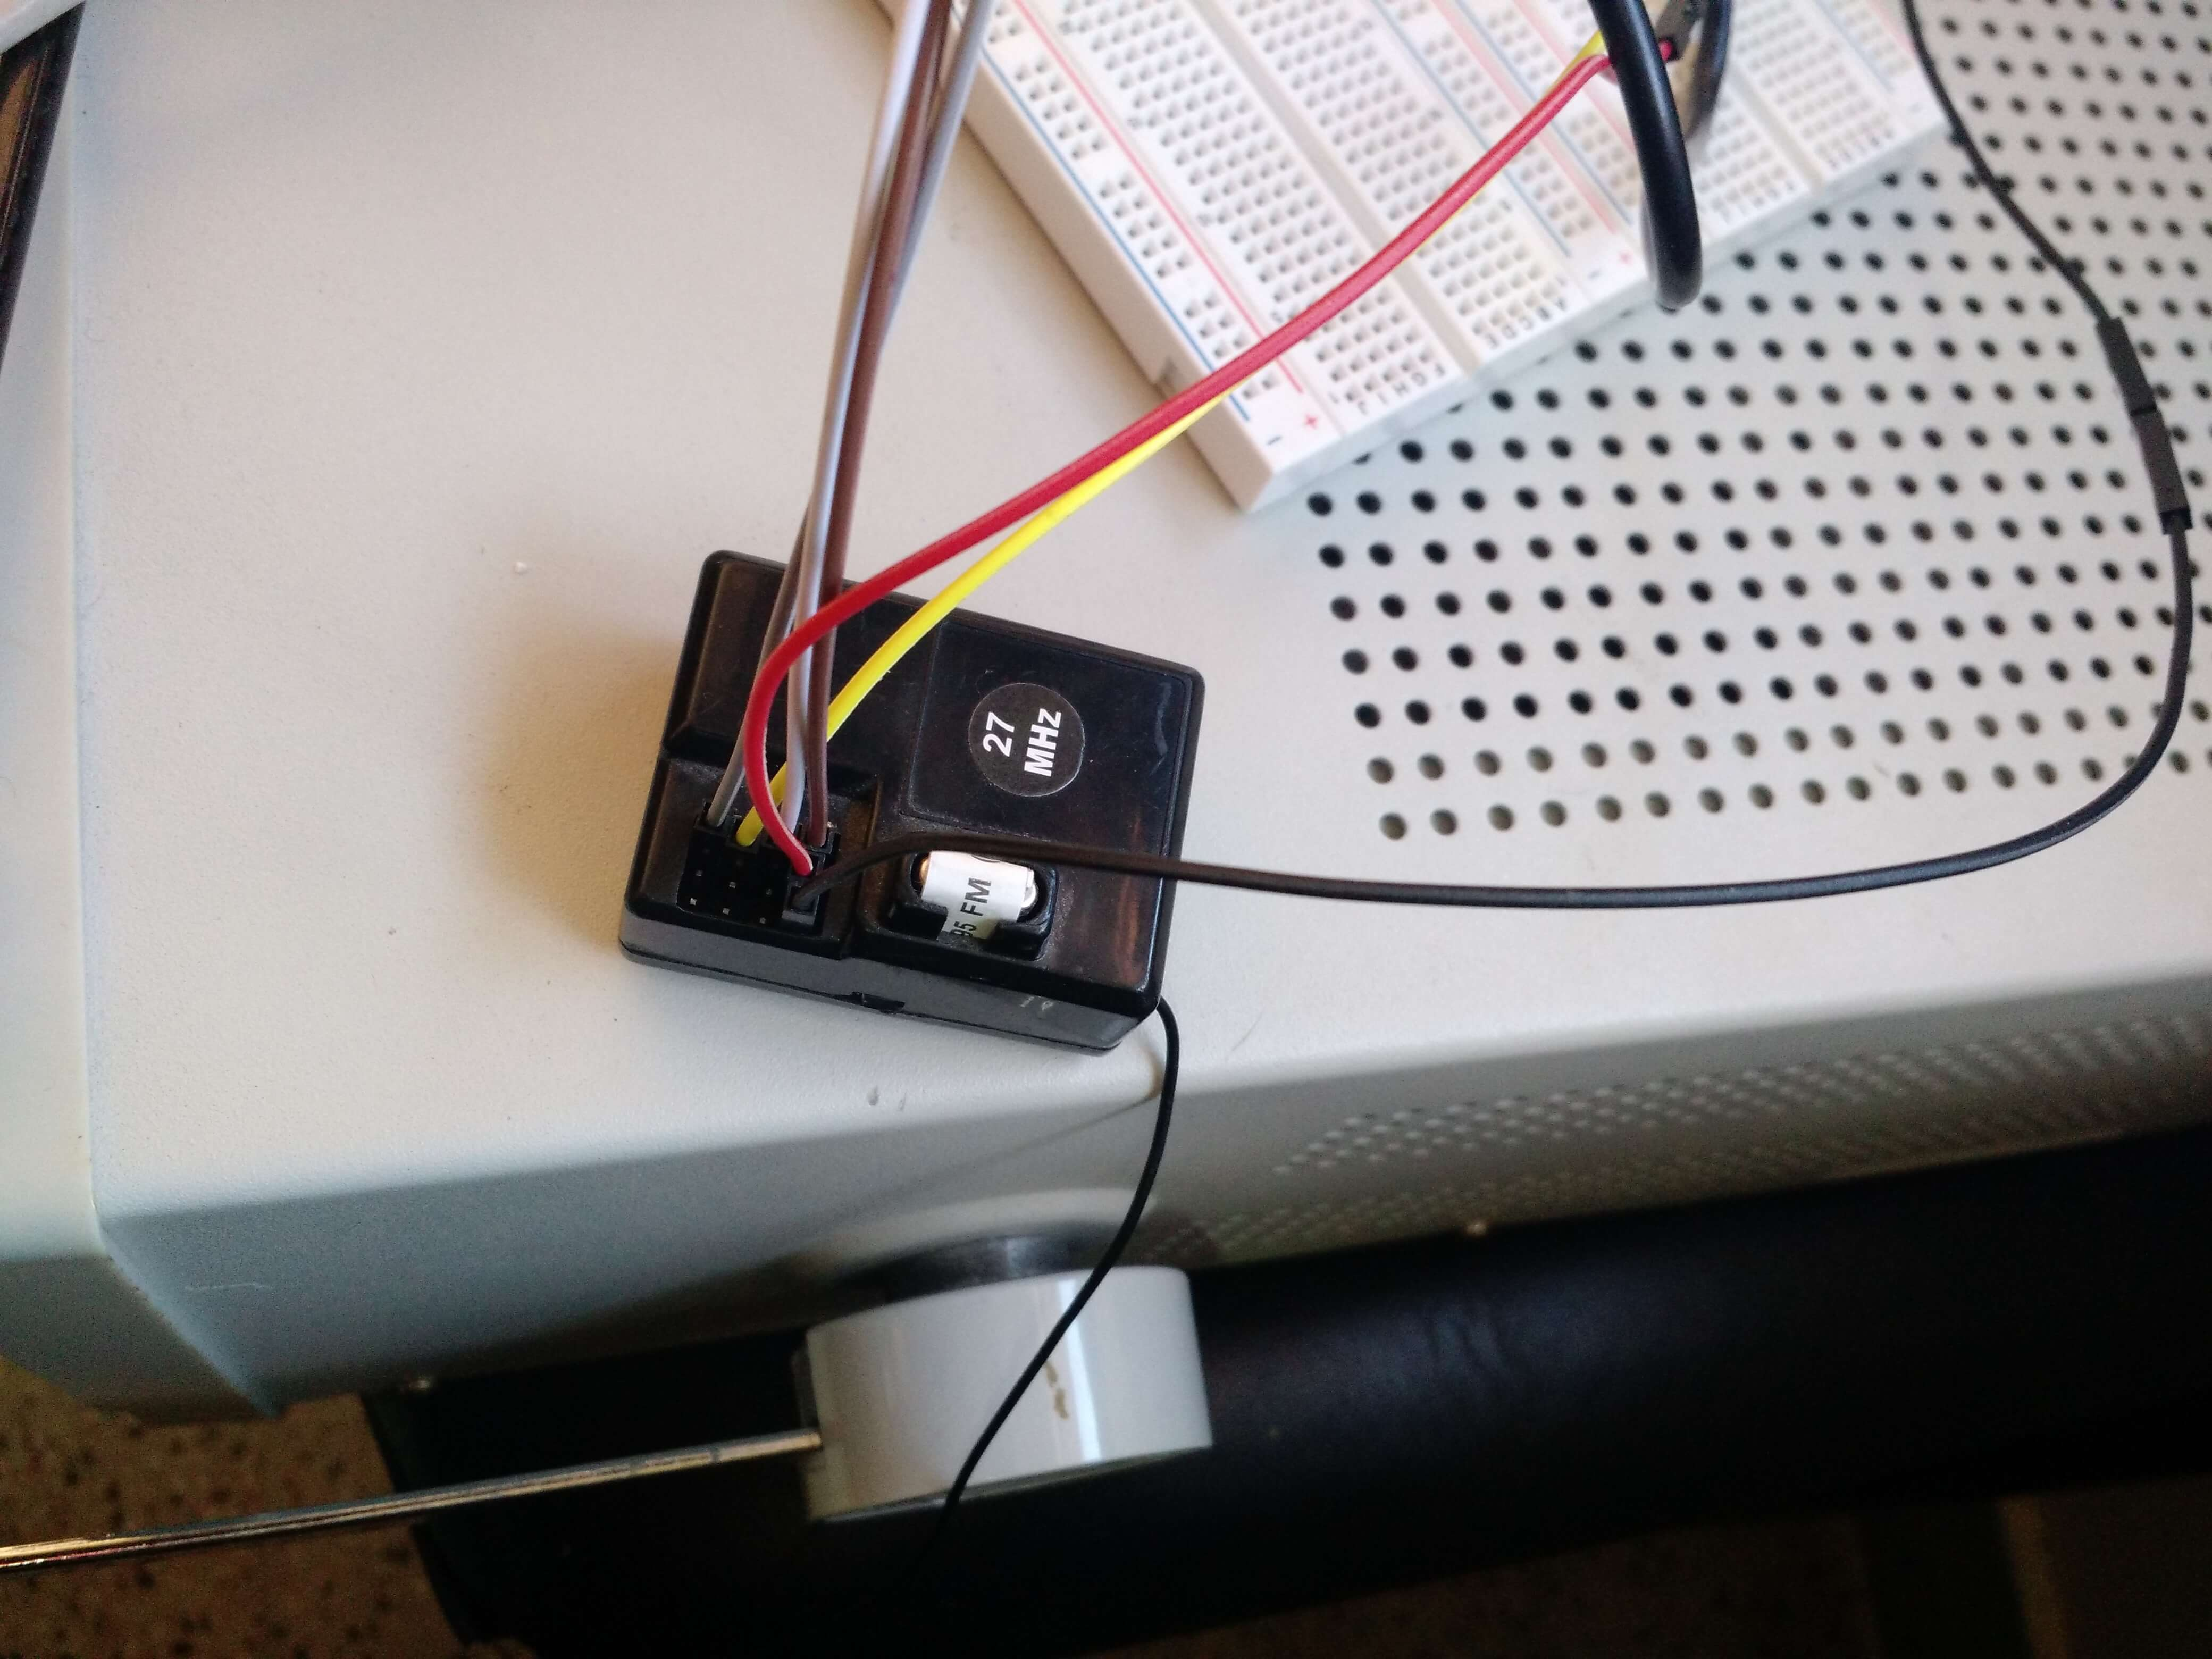
\includegraphics[width=0.5\linewidth, height=0.3\textheight]{Imagenes/fotos/rc_receptor}
		\caption{Receptor o Rx de 4 canales}
		\label{fig:rc_receptor}
		\end{figure}
		
		\begin{figure}[h!]
		\centering
		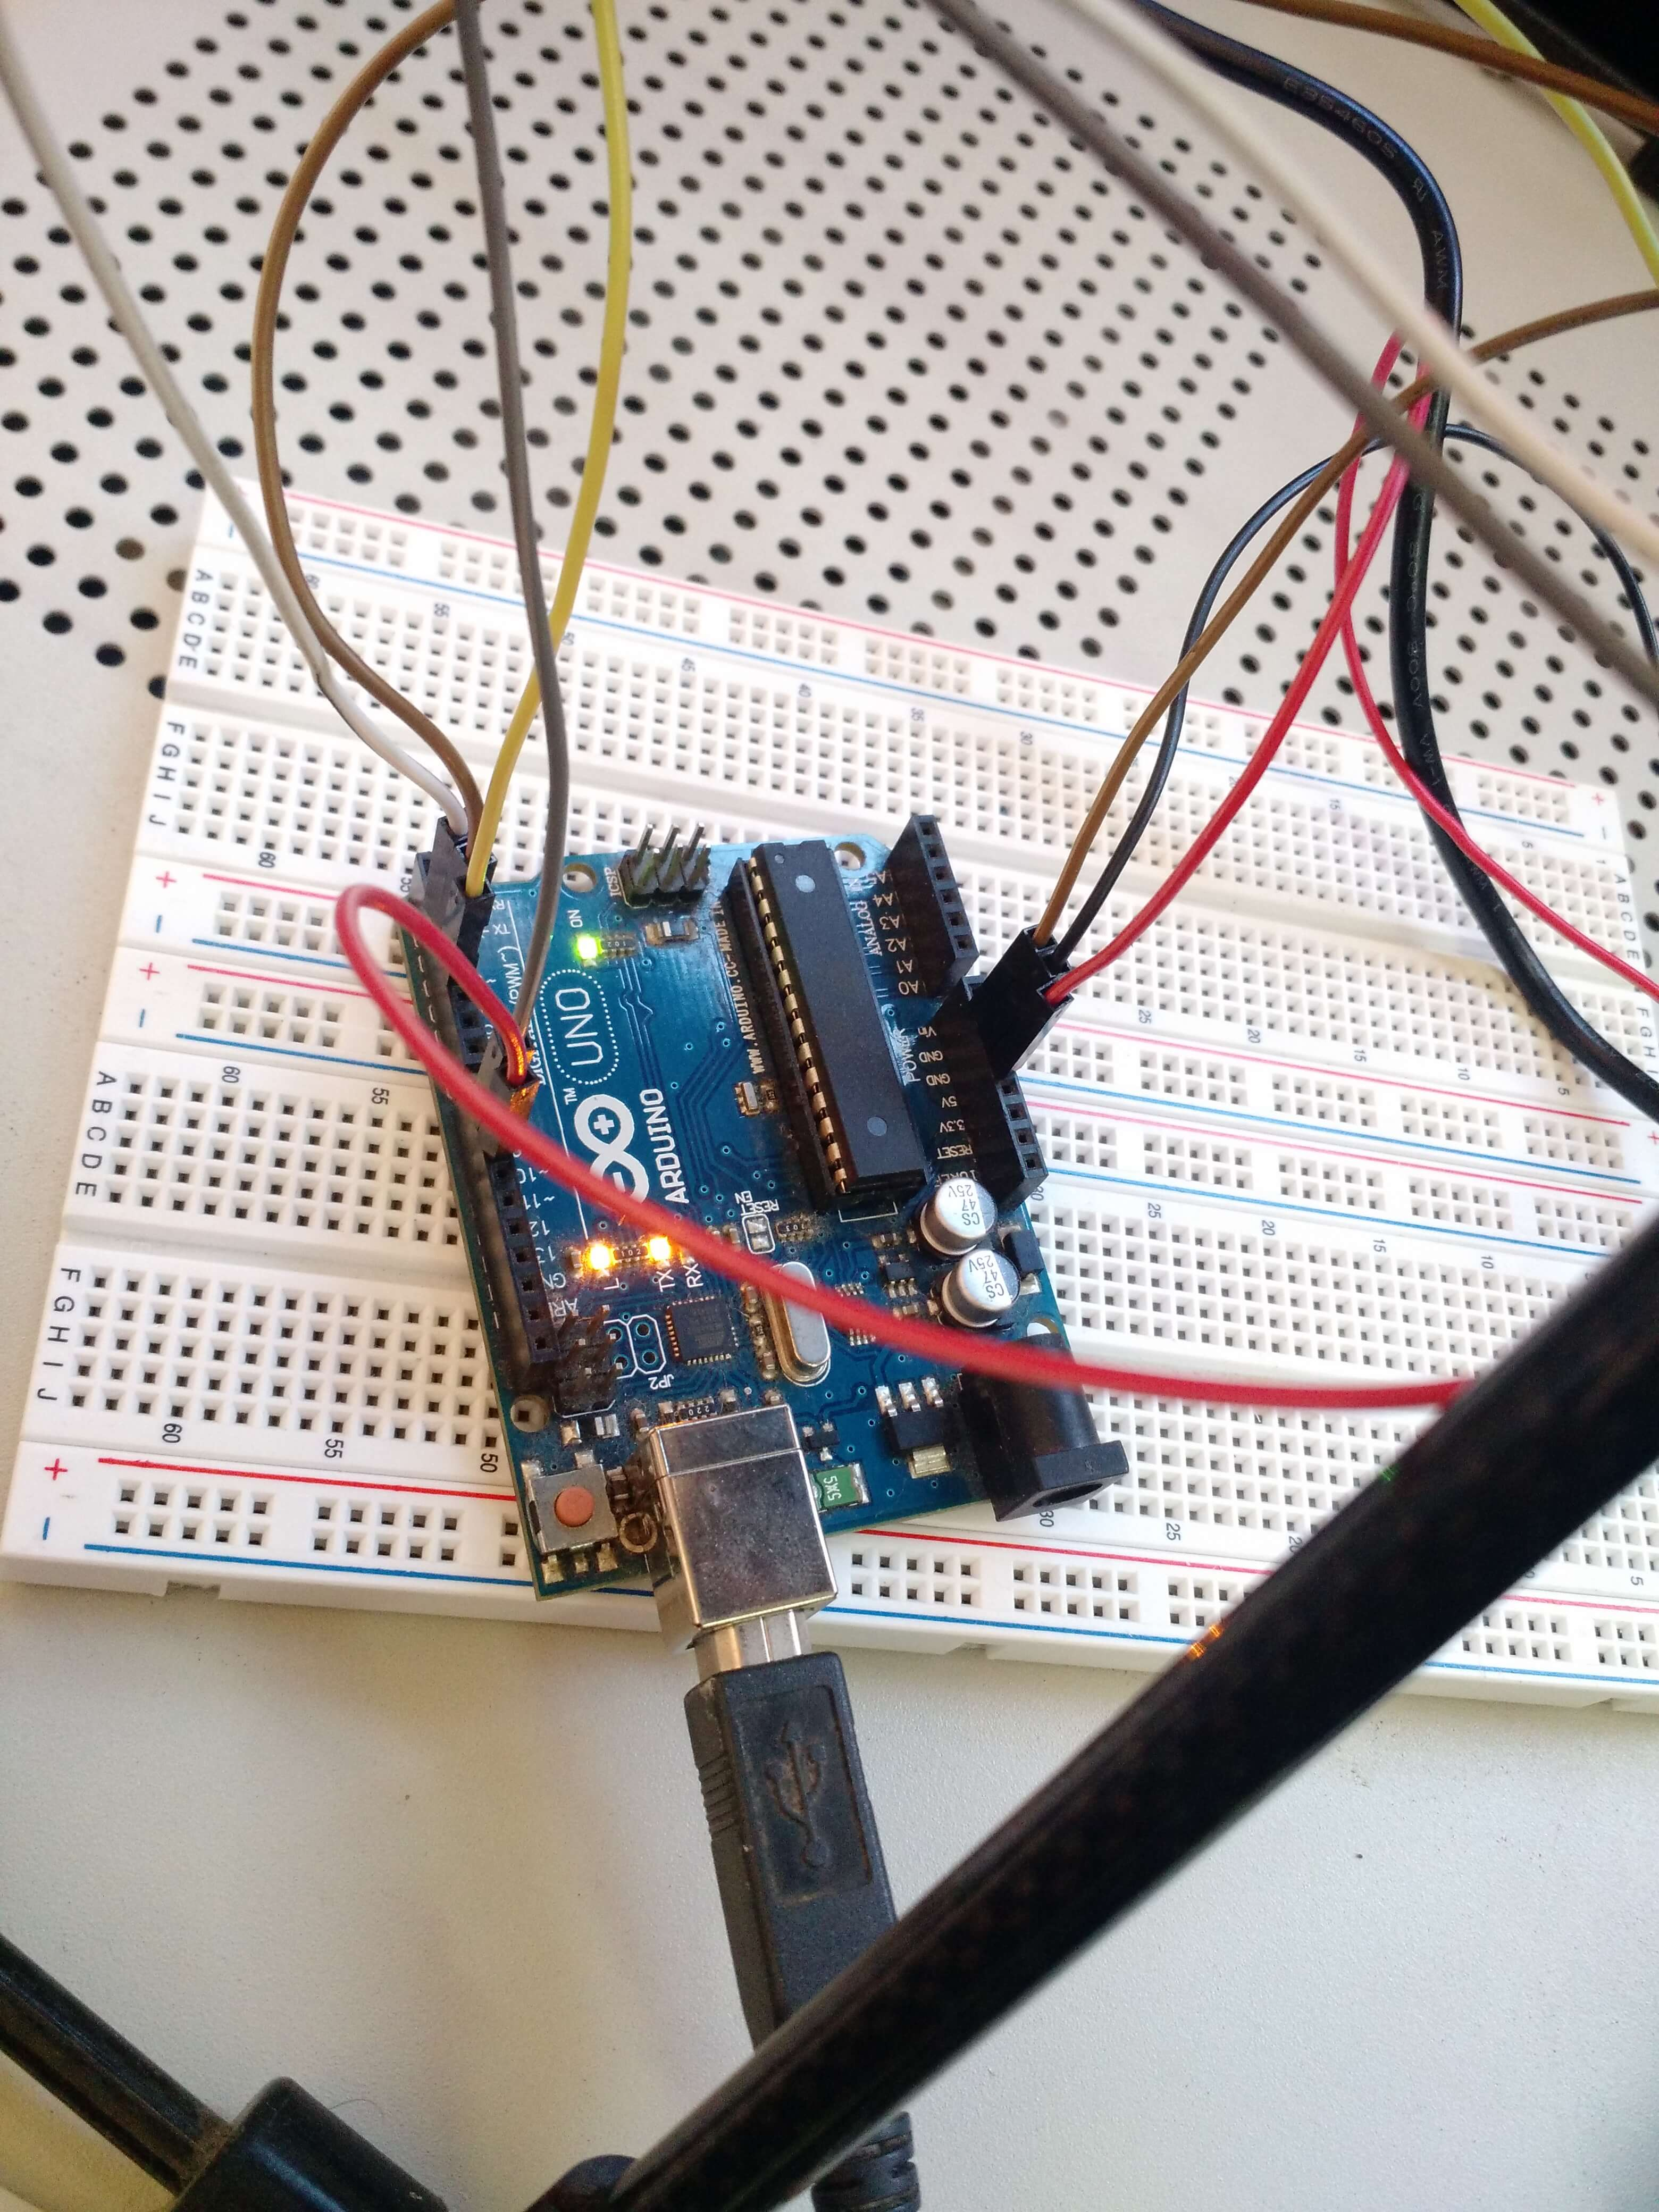
\includegraphics[width=0.5\linewidth, height=0.3\textheight]{Imagenes/fotos/arduino_ppm}
		\caption{Codificador PWM a SBUS implementado sobre Arduino.}
		\label{fig:arduino_ppm}
		\end{figure}
		
		
		\par Con respecto a las conexiones el�ctricas que lleva el cuadric�ptero, recurrimos en basarnos en la Figura \ref{fig:instnavio1}, donde muestra gr�ficamente el orden que llevan las conexiones con sus respectivos cables de colores. 
		
		\begin{figure}[h!]
		%TODO: Modificar imagen (esta mal el cableado de alimentacion de los motores)
		\centering
		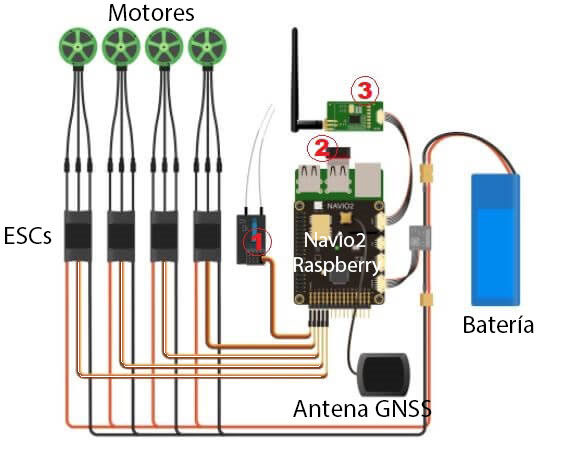
\includegraphics[width=0.9\linewidth, height=0.4\textheight]{Imagenes/inst_navio1}
		\caption{Esquema de conexiones}
		\label{fig:instnavio1}
		\end{figure}
		
		Un aspecto a tener en cuenta es que no todos los componentes que se visualizan en la Figura \ref{fig:instnavio1} est�n presentes al momento de la instrumentaci�n ya que los dispositivos marcados con los n�meros (1,2 y 3) son de tipo comunicaci�n y se supone que con el m�dulo interno de \textit{Wifi} podr�amos sustituir estos elementos. 
		\par Por lo tanto se procede a realizar las conexiones mostradas. En primera medida se inicia conectando los motores del cuerpo del cuadric�ptero con los pines de la Navio2 como se puede observar en la imagen \ref{fig:conexionmotores}
		
		\begin{figure}[h!]
			\centering
			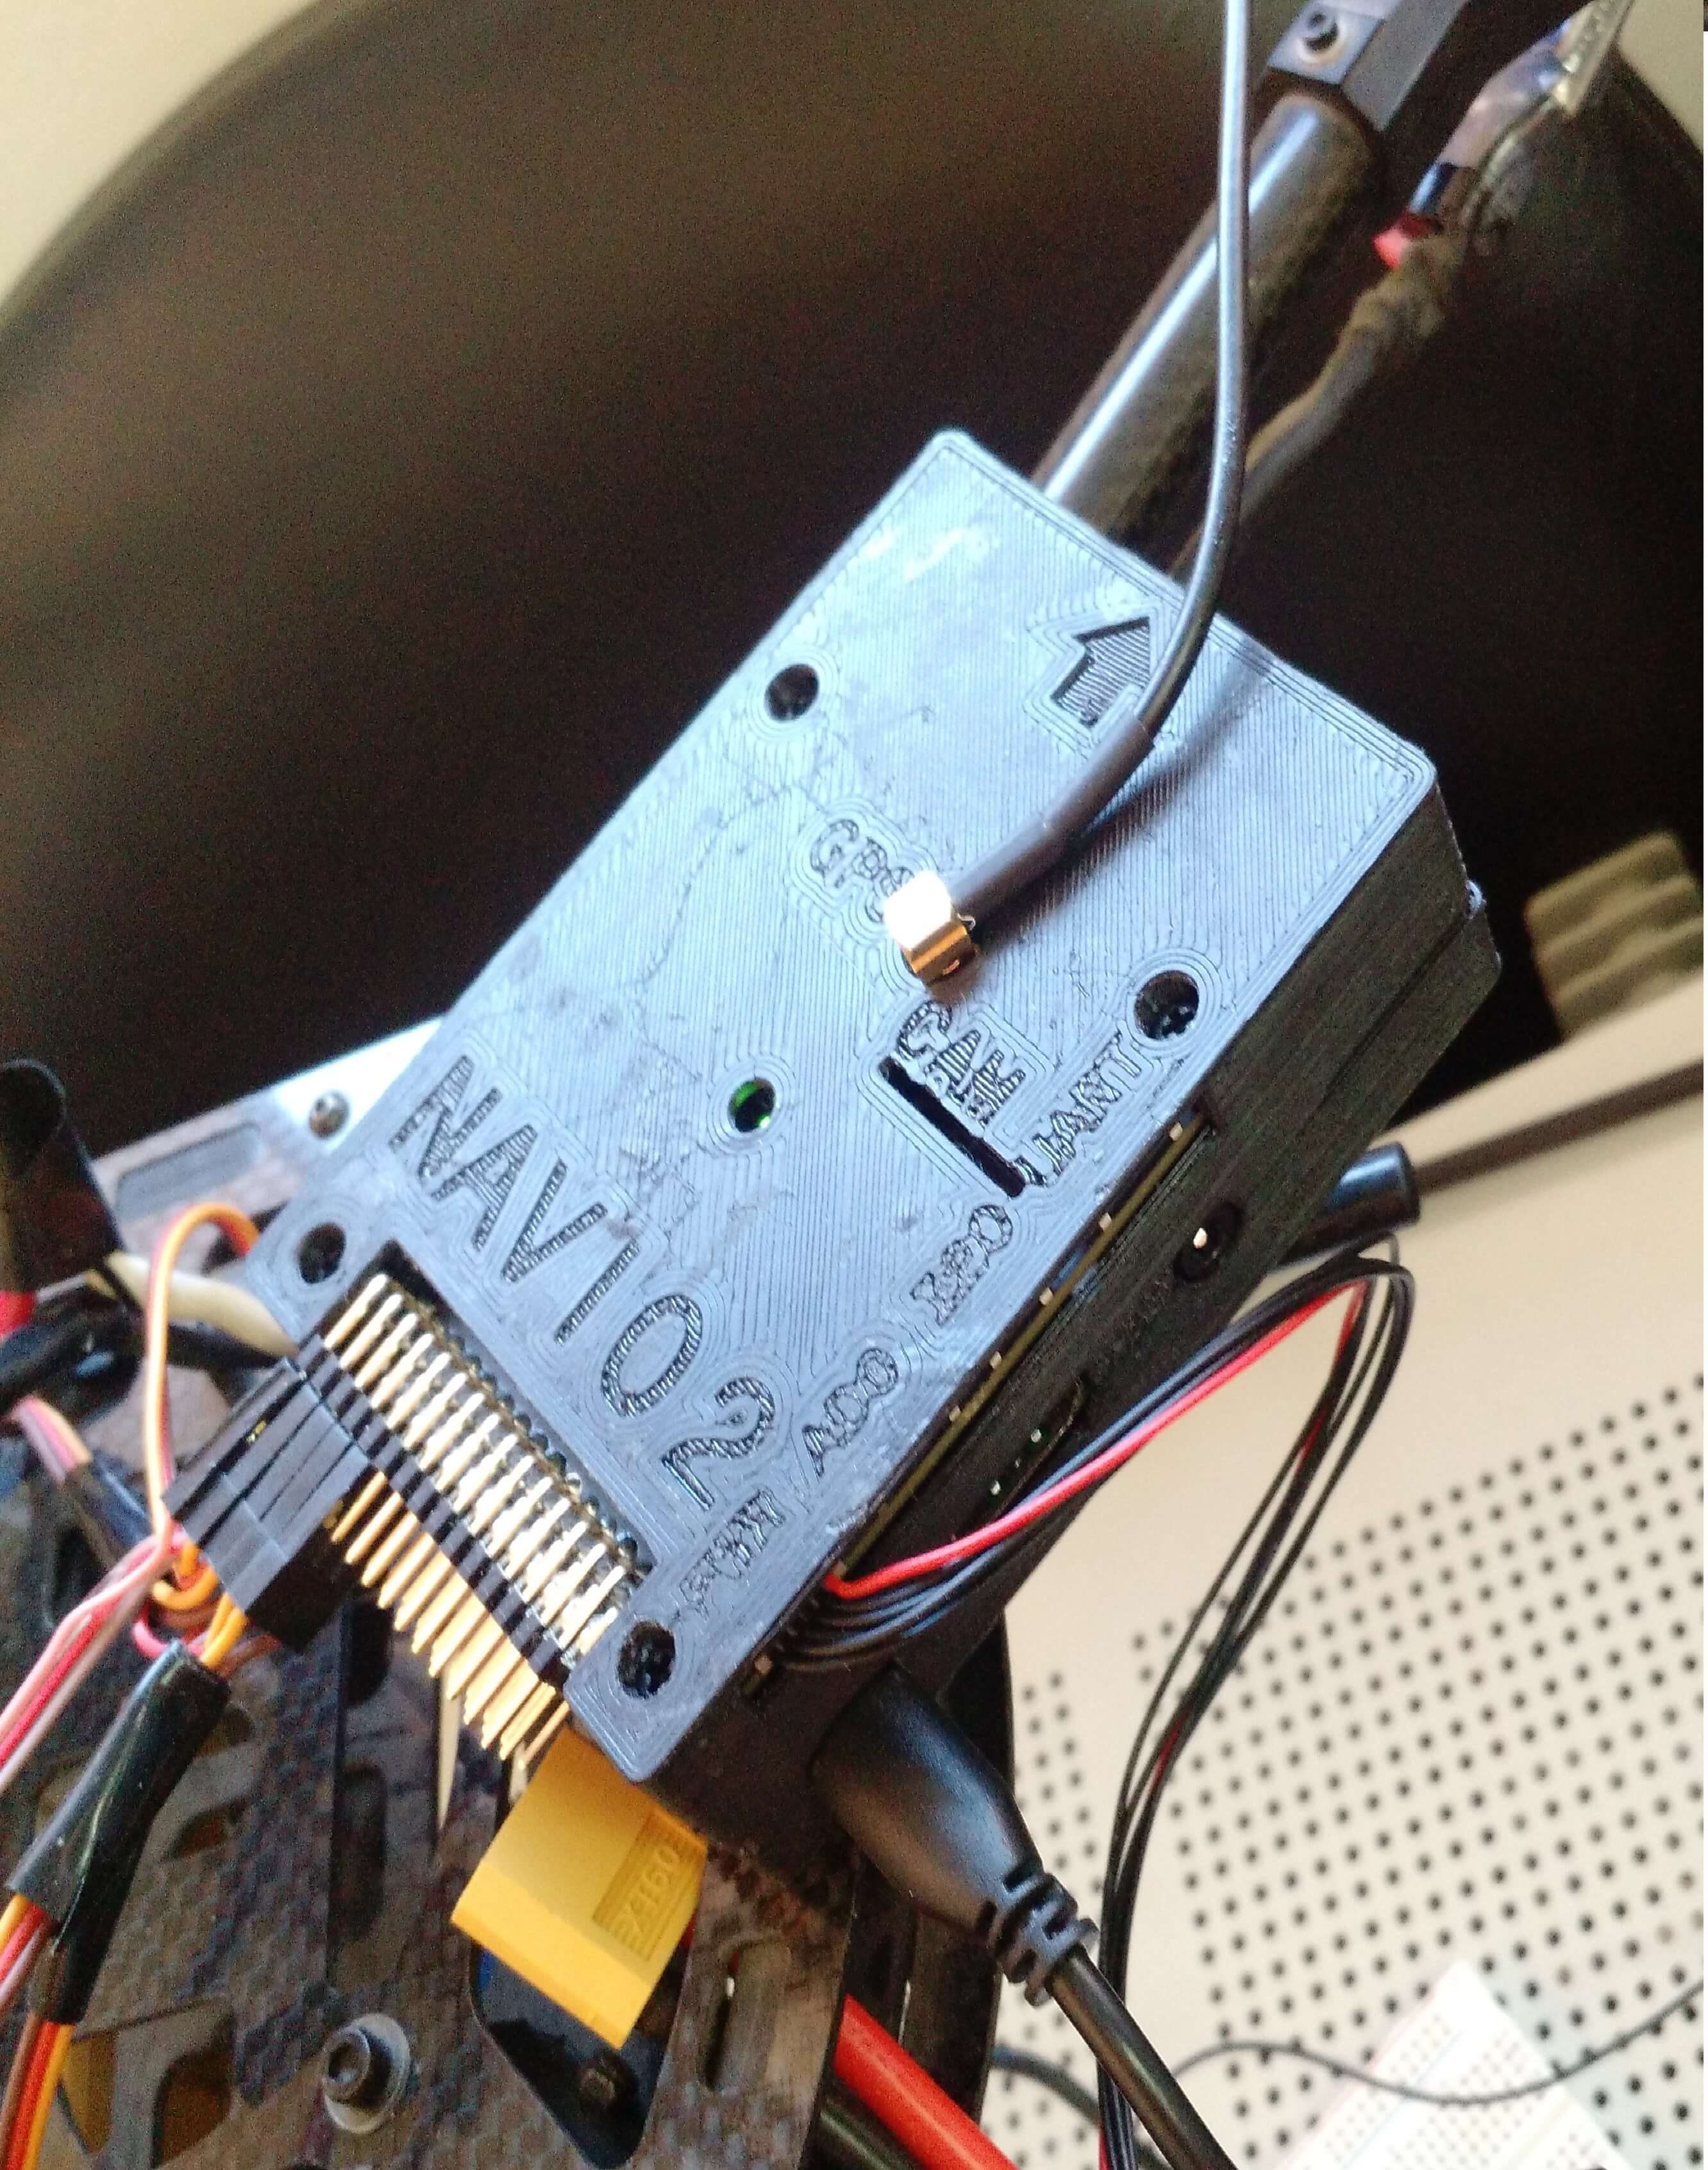
\includegraphics[width=0.4\linewidth, height=0.3\textheight]{Imagenes/fotos/conexion_motores}
			\caption{Conexi�n de datos a los motores.}
			\label{fig:conexionmotores}
		\end{figure}
		
		Despu�s de haber hecho las conexiones correspondientes a los motores, es necesario suministrarle energ�a de alg�n tipo de fuente para realizar las pruebas iniciales, es por eso que antes de conectar la bateria LiPo se considera la siguiente cuesti�n: ya que esta tiene una carga �til limitada se decide utilizar una fuente variable regulable disponible en el laboratorio de electr�nica del \textit{sinc(i)}  con el objetivo de realizar las pruebas necesarias sin estar dependiendo de la carga de la bater�a. Antes de realizar la conexi�n se ajusta el voltaje seg�n la bater�a Lipo existente (12V), dejando libre la cantidad de Amperes para que consuma lo que necesite. La fuente utilizada se puede observar en la Figura  \ref{fig:fuentevr}
		
		\begin{figure}[h!]
		\centering
		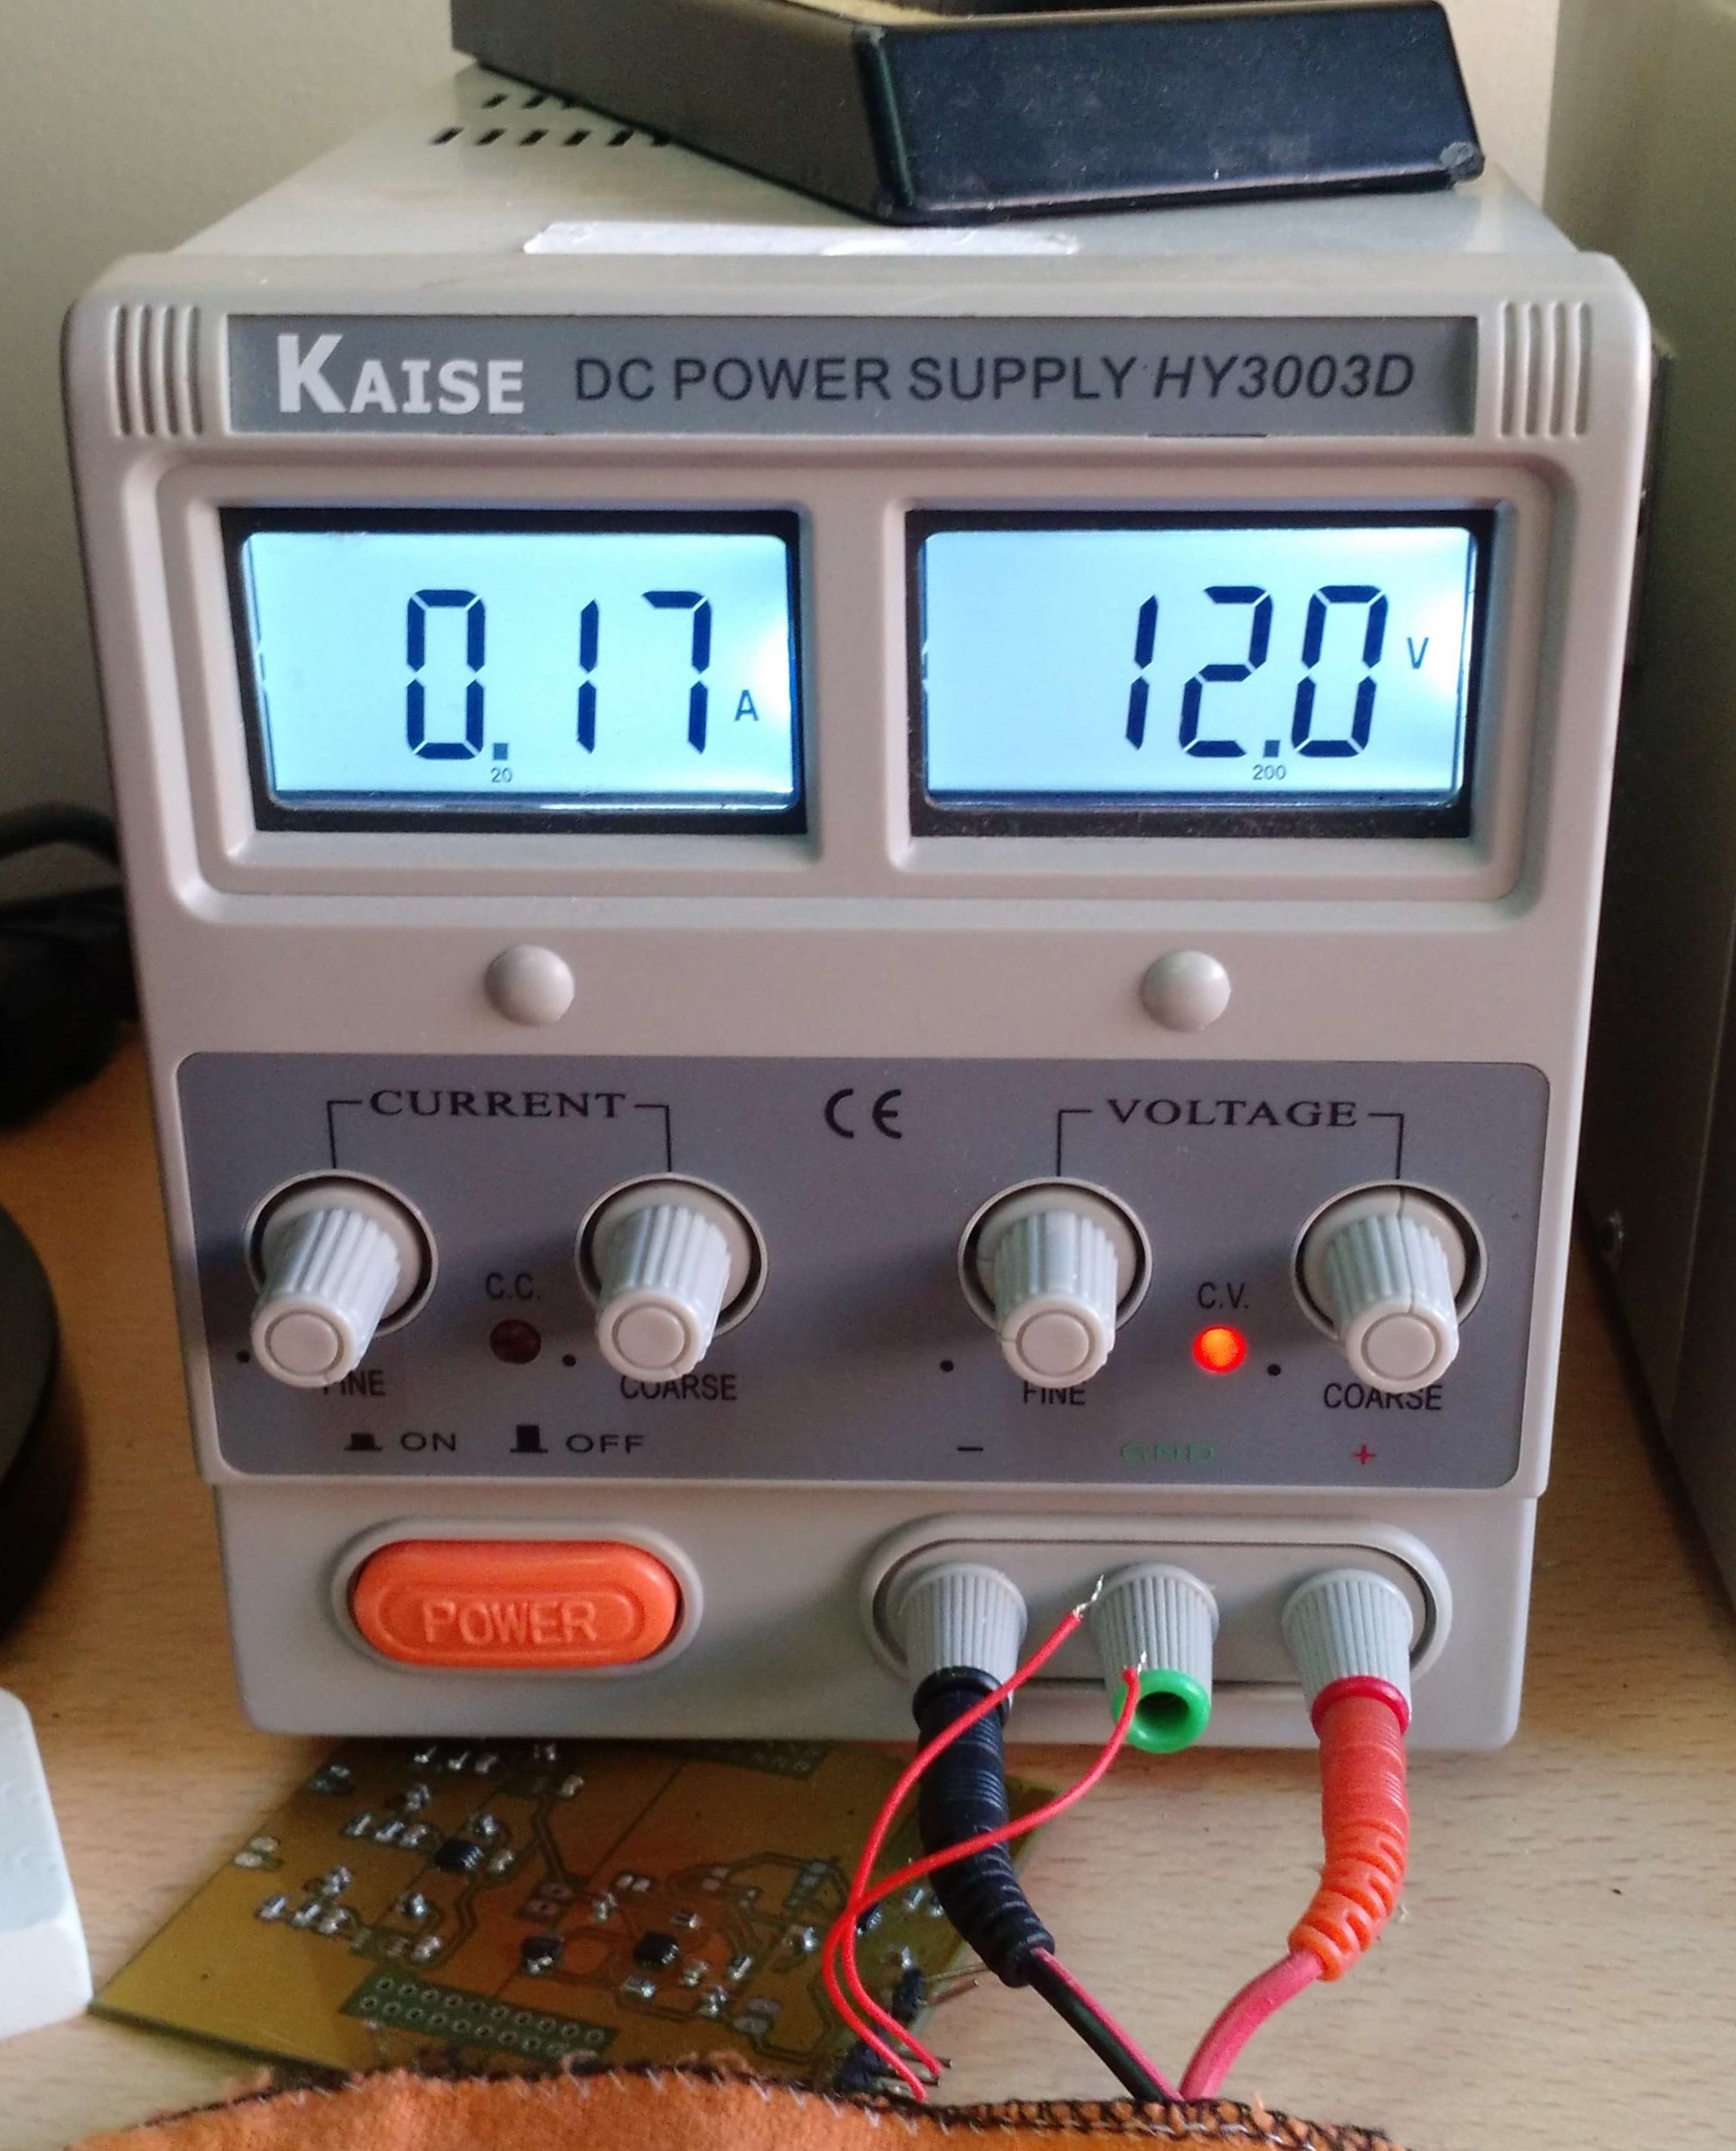
\includegraphics[width=0.4\linewidth, height=0.3\textheight]{Imagenes/fotos/fuentevr}
		\caption{Fuente variable regulable.}
		\label{fig:fuentevr}
		\end{figure}
		
		En la Figura \ref{fig:instnavio1} se puede ver que la bater�a suministra energ�a a los cuatro motores y al veh�culo, por lo tanto se decide alimentar al veh�culo con el transformador de f�brica y suministrar energ�a a  los motores con la fuente. Esta fuente como se puede observar en la Figura \ref{fig:fuentevr} contiene un �nico par de salida (positivo y negativo) por lo que es necesario multiplexar esta salida a 4 par de salidas m�s. Para eso se decide armar y soldar un conjunto de cables con sus respectivos conectores quedando de la siguiente manera.

%\begin{figure}[h!]
%\centering
%\includegraphics[width=0.5\linewidth, height=0.4\textheight]{Imagenes/fotos/IMG_20170601_131119448}
%\caption{Multiplexor}
%\label{fig:img20170601131119448}
%\end{figure}

Por �ltimo, se verifican las conexiones pertinentes a los planos y se buscan imperfectos en las uniones, en caso de encontrar alg�n tipo de estos se procede a repararlos. 
\begin{figure}[h!]
\centering
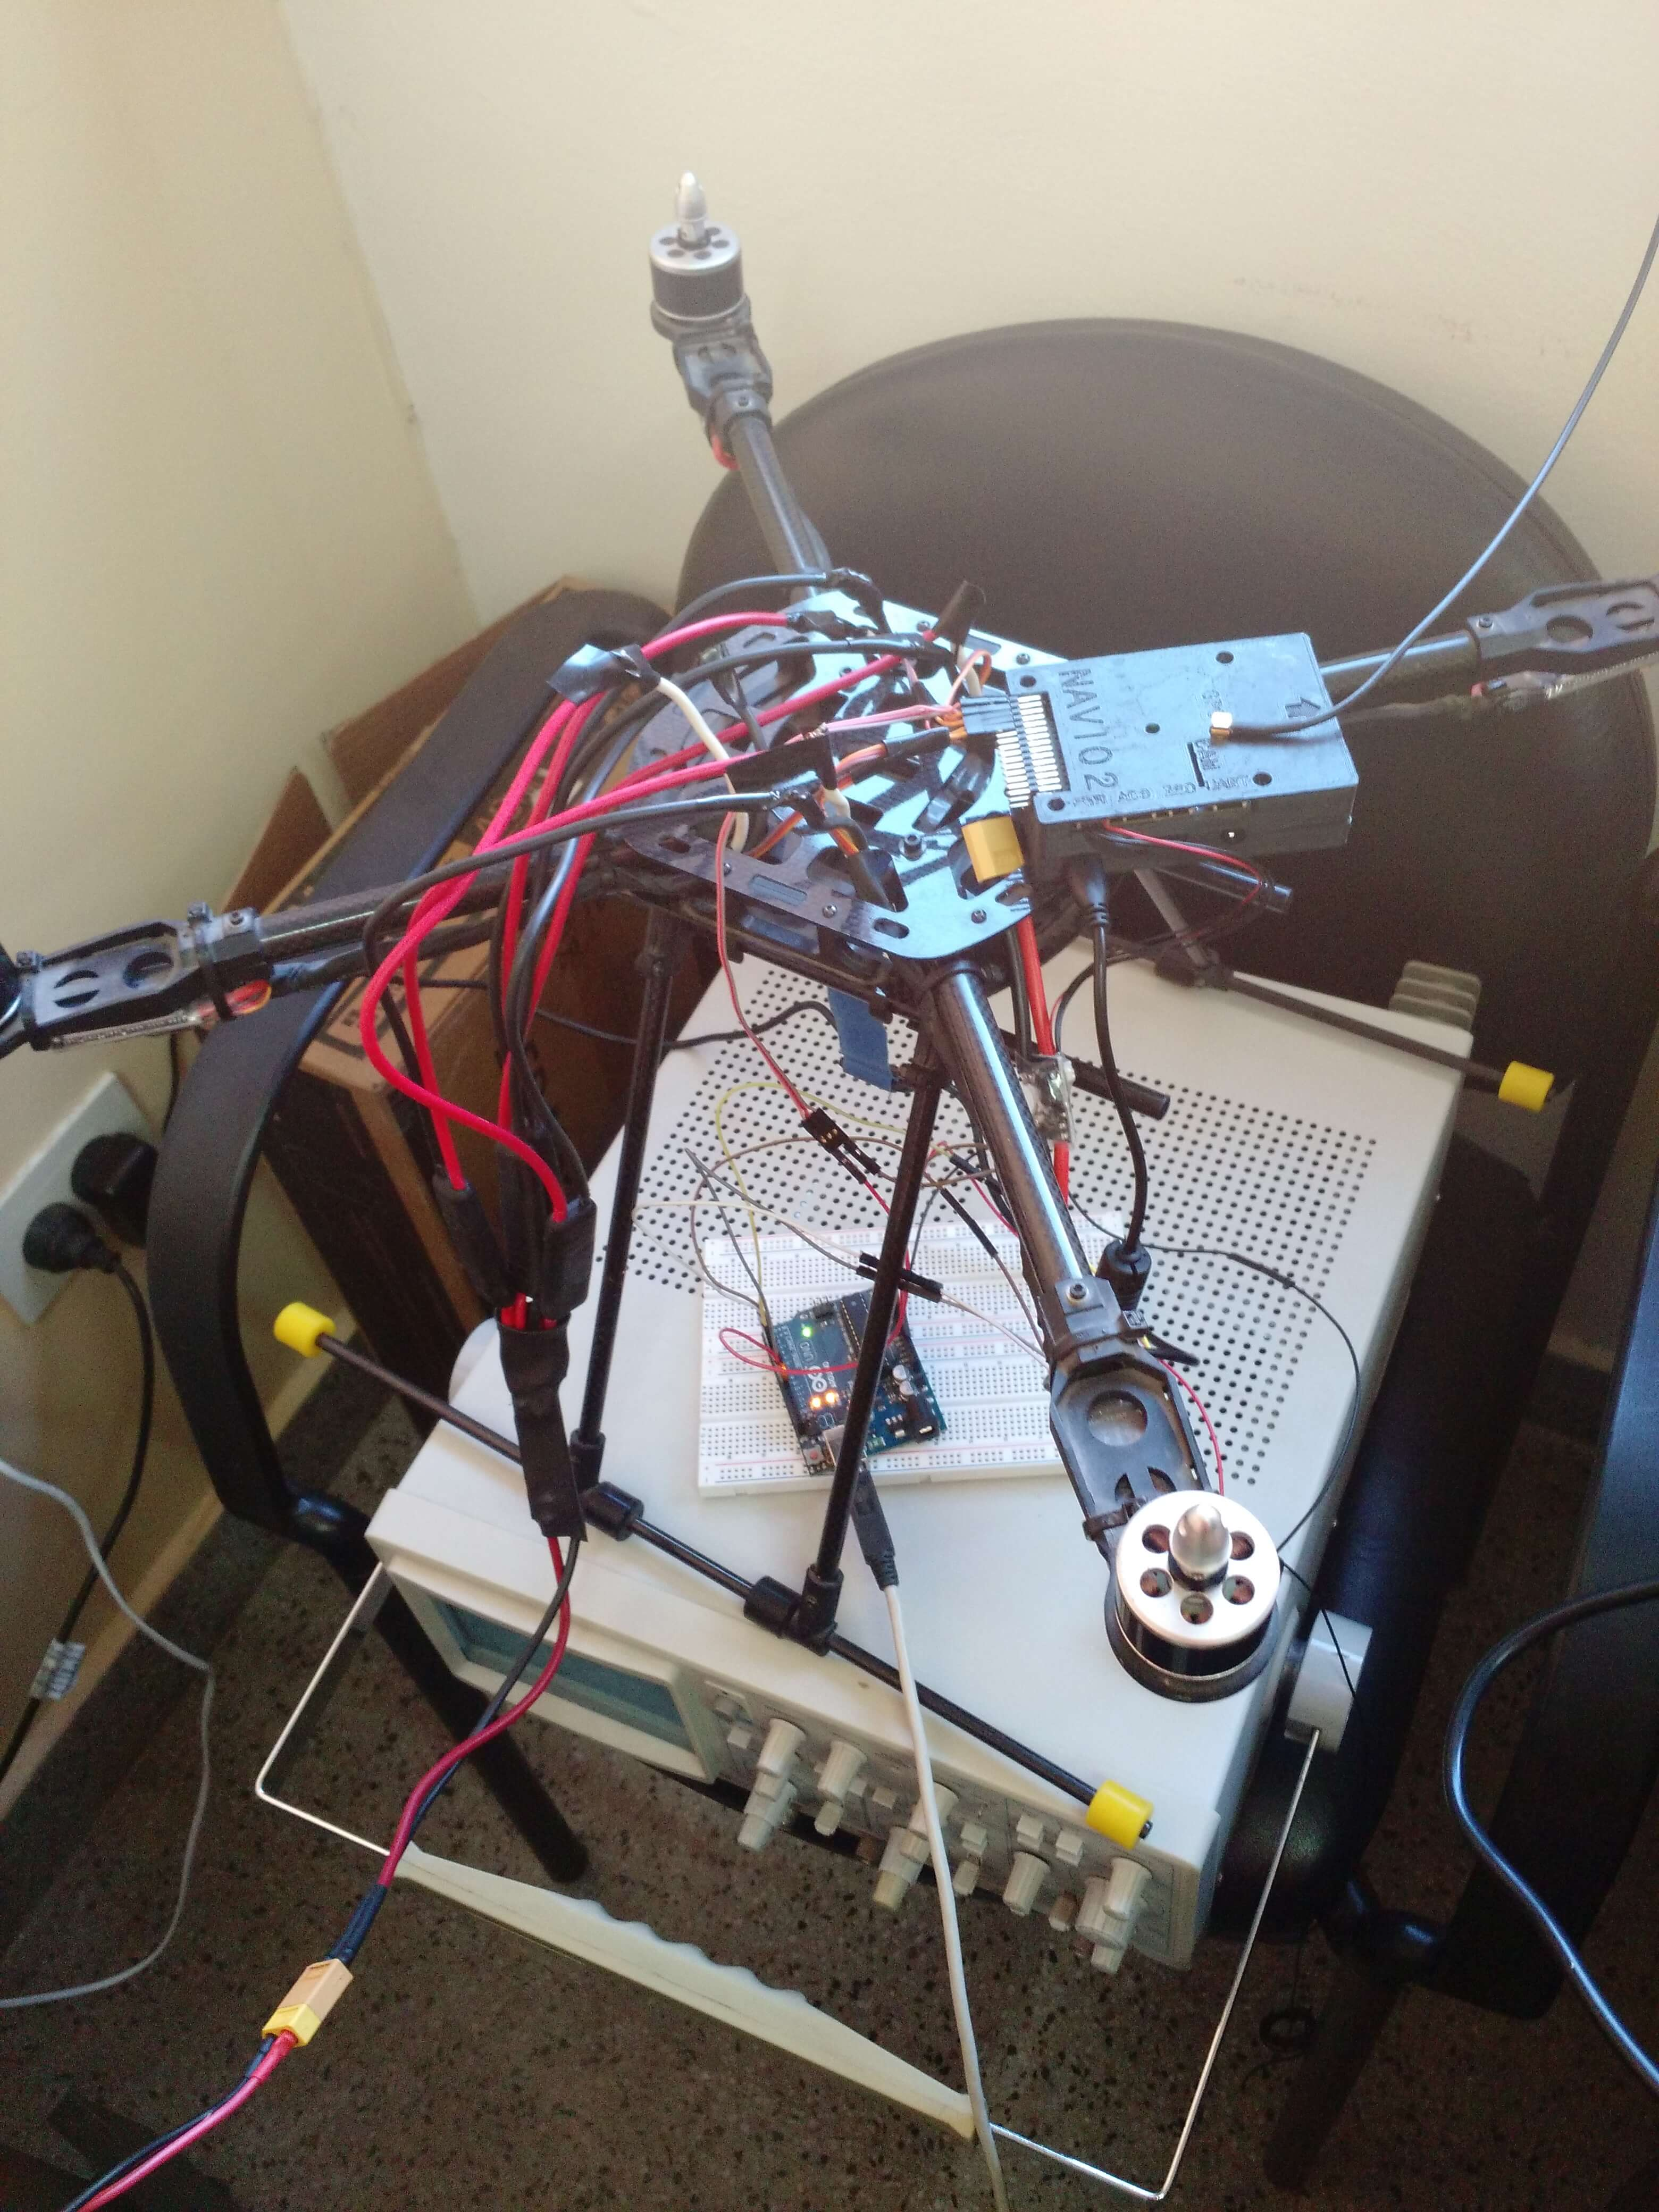
\includegraphics[width=0.5\linewidth, height=0.4\textheight]{Imagenes/fotos/quad_armado}
\caption{Cuadric�ptero armado para verificar funcionamiento.}
\label{fig:terminado}
\end{figure}


\subsection{Prueba de funcionamiento inicial}
Como etapa final y con el objetivo de verificar el correcto funcionamiento de nuestro veh�culo, se inicia el proceso de calibraci�n de sensores, para eso se decide utilizar \textbf{Mavproxy} seleccionando el m�dulo de calibraci�n y consecuentemente realizando los pasos que se nos indican de manera sencilla como se puede observar en la Figura \ref{fig:calibmavproxy}. 

Una vez concluida la etapa de calibraci�n se procede a enviar misiones de prueba, como por ejemplo elevarse del suelo 1 metro desde la posici�n inicial sin tener instalado las h�lices por motivos de seguridad, d�ndonos como resultados que el veh�culo interpreta los comandos. Aunque estas pruebas fueron realizadas de modo superficial en el capitulo \ref{cap4:pruebas} se profundizar� que el funcionamiento integral de los componentes responda de manera correcta.


\begin{figure}[h!]
\centering
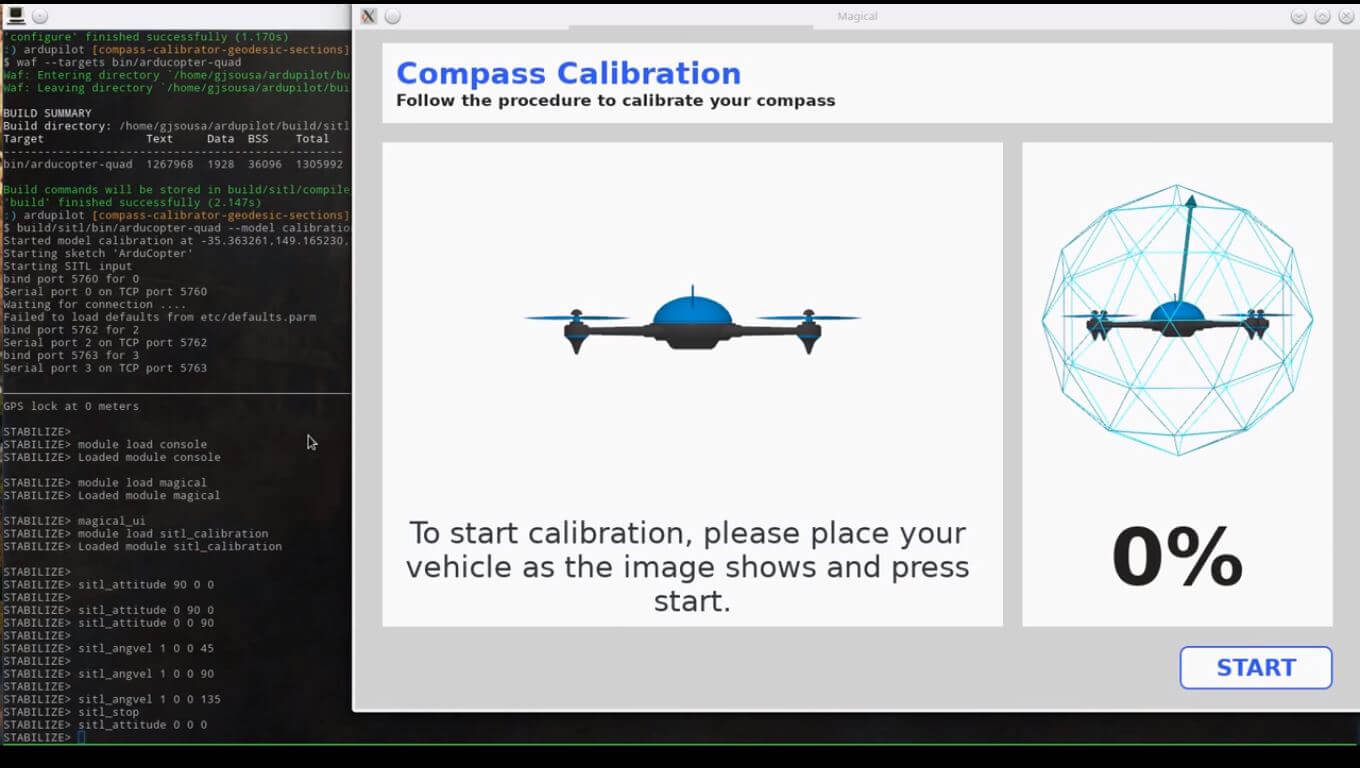
\includegraphics[width=0.8\linewidth, height=0.4\textheight]{Imagenes/calibMavproxy}
\caption{Ejecuci�n del modulo de calibraci�n de MavProxy}
\label{fig:calibmavproxy}
\end{figure}


% Variable local para emacs, para  que encuentre el fichero maestro de
% compilaci�n y funcionen mejor algunas teclas r�pidas de AucTeX
%%%
%%% Local Variables:
%%% mode: latex
%%% TeX-master: "../ManualTeXiS.tex"
%%% End:
    % Gesti�n del hardware y armado 
% -*-coding: iso-latin-1  -*-
%---------------------------------------------------------------------
%
%                          Cap�tulo 2
%
%---------------------------------------------------------------------
%
% 02EstructuraYGeneracion.tex
% Copyright 2009 Marco Antonio Gomez-Martin, Pedro Pablo Gomez-Martin
%
% This file belongs to the TeXiS manual, a LaTeX template for writting
% Thesis and other documents. The complete last TeXiS package can
% be obtained from http://gaia.fdi.ucm.es/projects/texis/
%
% Although the TeXiS template itself is distributed under the 
% conditions of the LaTeX Project Public License
% (http://www.latex-project.org/lppl.txt), the manual content
% uses the CC-BY-SA license that stays that you are free:
%
%    - to share & to copy, distribute and transmit the work
%    - to remix and to adapt the work
%
% under the following conditions:
%
%    - Attribution: you must attribute the work in the manner
%      specified by the author or licensor (but not in any way that
%      suggests that they endorse you or your use of the work).
%    - Share Alike: if you alter, transform, or build upon this
%      work, you may distribute the resulting work only under the
%      same, similar or a compatible license.
%
% The complete license is available in
% http://creativecommons.org/licenses/by-sa/3.0/legalcode
%
%---------------------------------------------------------------------

% -------------------------------------------------------------------------------
%      Estilos para los segmentos de c�digos/comandos para aparentar una consola
% -------------------------------------------------------------------------------

\definecolor{gray97}{gray}{.97}
\definecolor{gray75}{gray}{.75}
\definecolor{gray45}{gray}{.45}

\definecolor{mygray}{rgb}{0.4,0.4,0.4}
\definecolor{mygreen}{rgb}{0,0.8,0.6}
\definecolor{myorange}{rgb}{1.0,0.4,0}
\definecolor{gray97}{gray}{.97}
\definecolor{gray75}{gray}{.75}
\definecolor{gray45}{gray}{.45}

\lstset{ 
	basicstyle=\footnotesize\sffamily\color{black},
	commentstyle=\color{mygray},
	frame=single,
	numbers=left,
	numbersep=5pt,
	numberstyle=\tiny\color{mygray},
	keywordstyle=\color{mygreen},
	showspaces=false,
	showstringspaces=false,
	stringstyle=\color{myorange},
	tabsize=2
}

% minimizar fragmentado de listados
\lstnewenvironment{listing}[1][]
{\lstset{#1}\pagebreak[0]}{\pagebreak[0]}

\lstdefinestyle{consola}
{basicstyle=\scriptsize\bf\ttfamily,
	backgroundcolor=\color{gray75},
}

\lstdefinestyle{Python}
{language=Python,
}


\lstset{ frame=Ltb,
	framerule=0pt,
	aboveskip=0.5cm,
	framextopmargin=3pt,
	framexbottommargin=4pt,
	framexleftmargin=0.4cm,
	framesep=0pt,
	rulesep=.4pt,
	backgroundcolor=\color{gray97},
	rulesepcolor=\color{black},
	%
	stringstyle=\ttfamily,
	showstringspaces = false,
	basicstyle=\small\ttfamily,
	commentstyle=\color{gray45},
	keywordstyle=\bfseries,
	%
	numbers=left,
	numbersep=15pt,
	numberstyle=\tiny,
	numberfirstline = false,
	breaklines=true,
}

\lstdefinestyle{consola}
{basicstyle=\scriptsize\bf\ttfamily,
	backgroundcolor=\color{gray75},
}




\chapter{Gesti�n de componentes y armado del cuadric�ptero}
\label{cap2:gest_y_arm}

\begin{FraseCelebre}
	
	\begin{Frase}
	 La mejor estructura no garantizar� los resultados ni el rendimiento.
	 Pero la estructura equivocada es una garant�a de fracaso.
	\end{Frase}

	\begin{Fuente}
		-Peter Drucker-
	\end{Fuente}

\end{FraseCelebre}

\begin{resumen}
Este cap�tulo contiene informaci�n sobre el procedimiento que se ha llevado a cabo en el desarrollo de la tercera etapa del proyecto. Esta etapa consiste principalmente en describir los pasos realizados para el armado del veh�culo a�reo no tripulado (VANT) de tipo cuadric�ptero. Adem�s, se incluir�n los inconvenientes que se han presentado en el transcurso del desarrollo del mismo con sus respectivas alternativas y/o soluciones. 

% TODO: Consultar si dejar esta parte   
\par Cabe mencionar que el hardware aqu� descripto como tambi�n las herramientas utilizadas han sido proporcionadas por el\textit{ Centro de Investigaci�n en Se�ales, Sistemas e Inteligencia sinc(i)} con sede en la Facultad de Ingenier�a y Ciencias H�dricas de la Universidad Nacional del Litoral y todo procedimiento riesgoso para el alumno ha sido siempre supervisado bajo personal id�neo en el tema.

\end{resumen}

%-------------------------------------------------------------------
\section{Hardware}
%-------------------------------------------------------------------
\label{cap2:sec:hardware}

Antes de empezar con la descripci�n del armado de un VANT, es necesario tener en conocimiento el hardware que est� involucrado en el veh�culo y en consecuencia su funcionamiento, como por ejemplo, los sensores que forman parte del mismo y hacen que el cuadric�ptero pueda realizar un vuelo de manera segura y controlada, el tipo de estructura usado para soportar los motores, la tecnolog�a responsable de la comunicaci�n y el ordenador que procesar� toda esa informaci�n. Es por eso que iniciamos esta secci�n con una lista del hardware utilizado y su respectiva descripci�n:


\begin{enumerate}
	\item Estructura de veh�culo.
	\item Controlador Electr�nico de Velocidad.
	\item Motor sin escobillas.
	\item Raspberry Pi 3.
	\item Navio2.
	\item Arduino UNO \footnote{Estos dispositivos no han sido previstos y tampoco forman parte definitiva del proyecto, ya que han surgido para solventar problemas que surgieron en el transcurso de esta etapa. \label{footnote_hardware} }.
	\item Radio Control \footref{footnote_hardware}.
	\item Joystick.
	\item Router \footref{footnote_hardware}.
	\item M�dulos XBee
	\item Bateria LiPo.
\end{enumerate}




	\subsection{Estructura de veh�culo}

		La estructura del cuadric�ptero como se puede ver en la Figura \ref{fig:estrucuadricoptero} consta en su parte inferior de un pat�n de aterrizaje que cumplen la funci�n (como en los helic�pteros) de soportar el veh�culo cuando se apoye sobre tierra y mantener las h�lices lo m�s alejado posible de piso cuando se encuentra en reposo. En su parte superior proporciona una base donde es posible instalar los dispositivos electr�nicos que controlan al veh�culo. Por �ltimo, desde la base se extienden 4 brazos con la funci�n de ser soporte a los motores con sus respectivas h�lices y adem�s, en cada motor se le incluye su controlador electr�nico de velocidad o ESC (\textit{Electronic Speed Controller}). 




		\begin{figure}[h!]
			\centering
			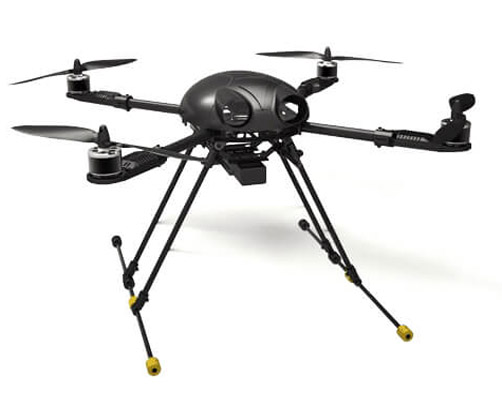
\includegraphics[width=0.4\linewidth, height=0.25\textheight]{Imagenes/estrucuadricoptero}
			\caption{Estructura cuadric�ptero de fibra de carbono}
			\label{fig:estrucuadricoptero}
		\end{figure}

		El material del cuerpo de veh�culo esta hecho con fibra de carbono \footnote{Aunque el mismo puede ser reemplazado por otro tipo de estructura, por ejemplo, un modelo impreso por una impresora 3D}, este consta con la propiedad de tener una elevada resistencia mec�nica que ser� de suma importancia ya que el veh�culo presenta altas probabilidades de sufrir alg�n choque o aterrizaje forzoso, adem�s de ser un material sumamente liviano por lo que disminuir� la fuerza de los motores para mantener un vuelo y por tanto, menos consumo de bater�a.
		

	\subsection{Controlador Electr�nico de Velocidad}
		Un controlador electr�nico de velocidad o por sus siglas en ingl�s \textit{Electronic Speed Control} como su nombre lo dice, es un circuito electr�nico con el prop�sito de variar la velocidad de un motor el�ctrico. Adem�s, por sus caracter�sticas puede funcionar como un freno din�mico.

		\begin{figure}[h!]
			\centering
			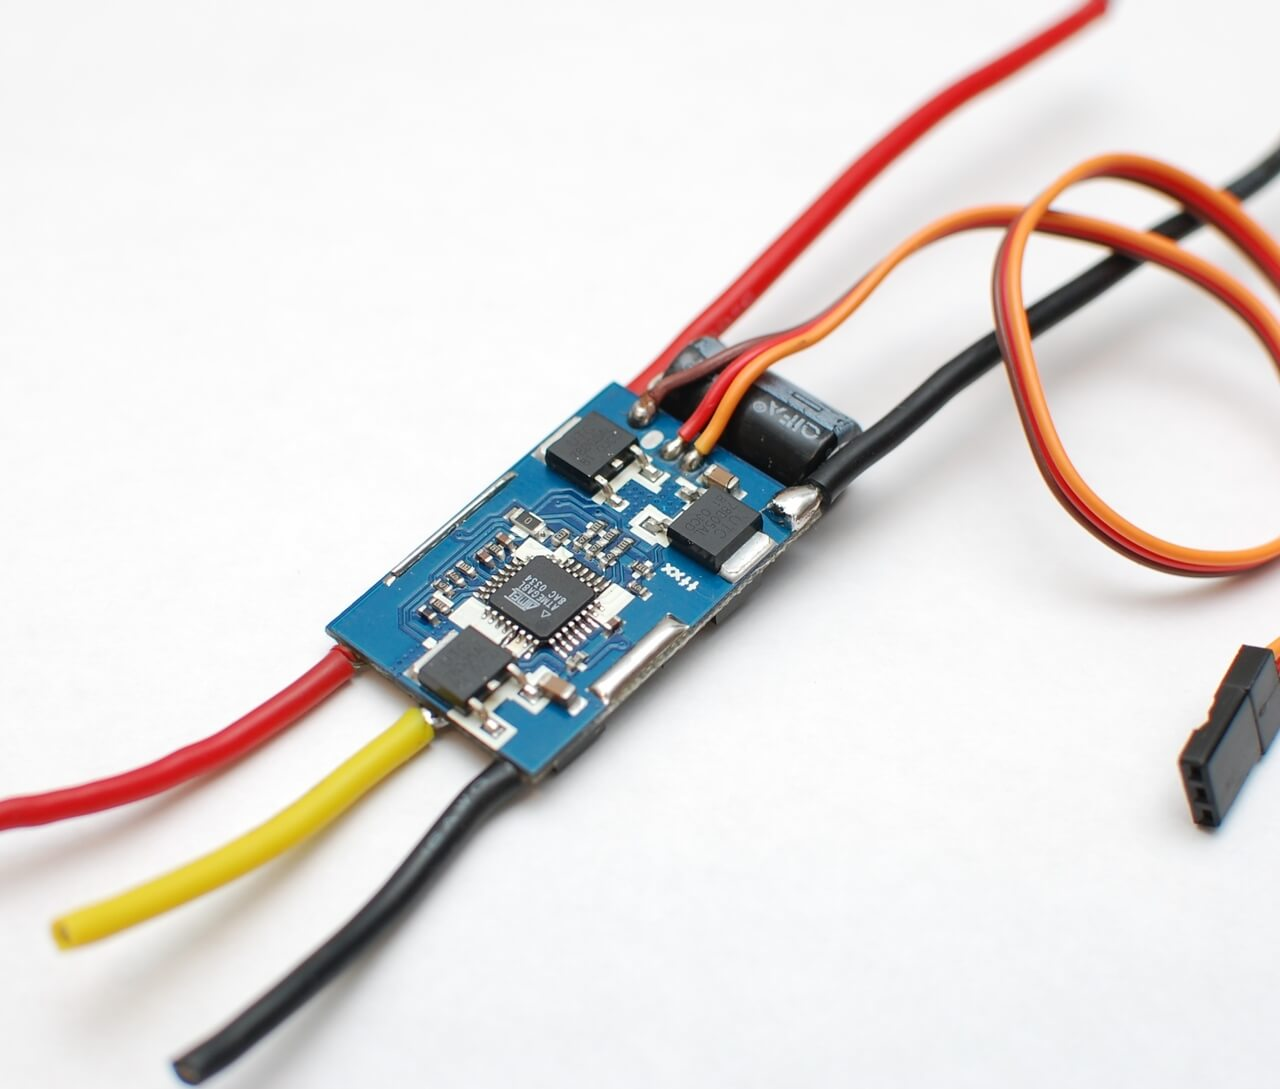
\includegraphics[width=0.4\linewidth, height=0.1\textheight]{Imagenes/esc}
			\caption{Controlador Electr�nico de Velocidad}
			\label{fig:esc}
		\end{figure}

	\subsection{Motores sin escobillas}
		Son los encargados de transformar la energ�a el�ctrica en mec�nica generando movimiento en las h�lices, y de esta manera dando propulsi�n al veh�culo para poder volar.

		\begin{figure}[h!]
			\centering
			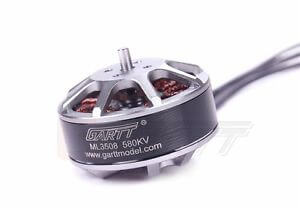
\includegraphics[width=0.4\linewidth, height=0.15\textheight]{Imagenes/motor}
			\caption{Motor sin escobillas}
			\label{fig:motor}
		\end{figure}

	\subsection{Raspberry Pi 3}
		Es un ordenador de tama�o reducido que trata de ofrecer las mismas funcionalidades y componentes que el de un ordenador com�n pero con un rendimiento menor, entre sus componentes, esta placa reducida tiene memoria RAM, GPU, puertos USB, HDMI, ranura para tarjeta SD, conector para una c�mara, conectividad WiFi, Ethernet, Bluetooth y 40 pines GPIO(\textit{General Purpose Input/Output}) donde es posible extender sus caracter�sticas instalando hardware extra como sensores, led, motores, interfaces, etc \cite{mcmanus2017raspberry}.
		\par \textbf{Especificaciones:}
			\begin{itemize}
				
				\item 1.2GHz 64-bit quad-core ARMv8 CPU
				\item 1GB RAM (Compartido con la GPU)
				\item GPU Broadcom VideoCore IV	\newline
			\end{itemize}
		
		\begin{figure}[h!]
			\centering
			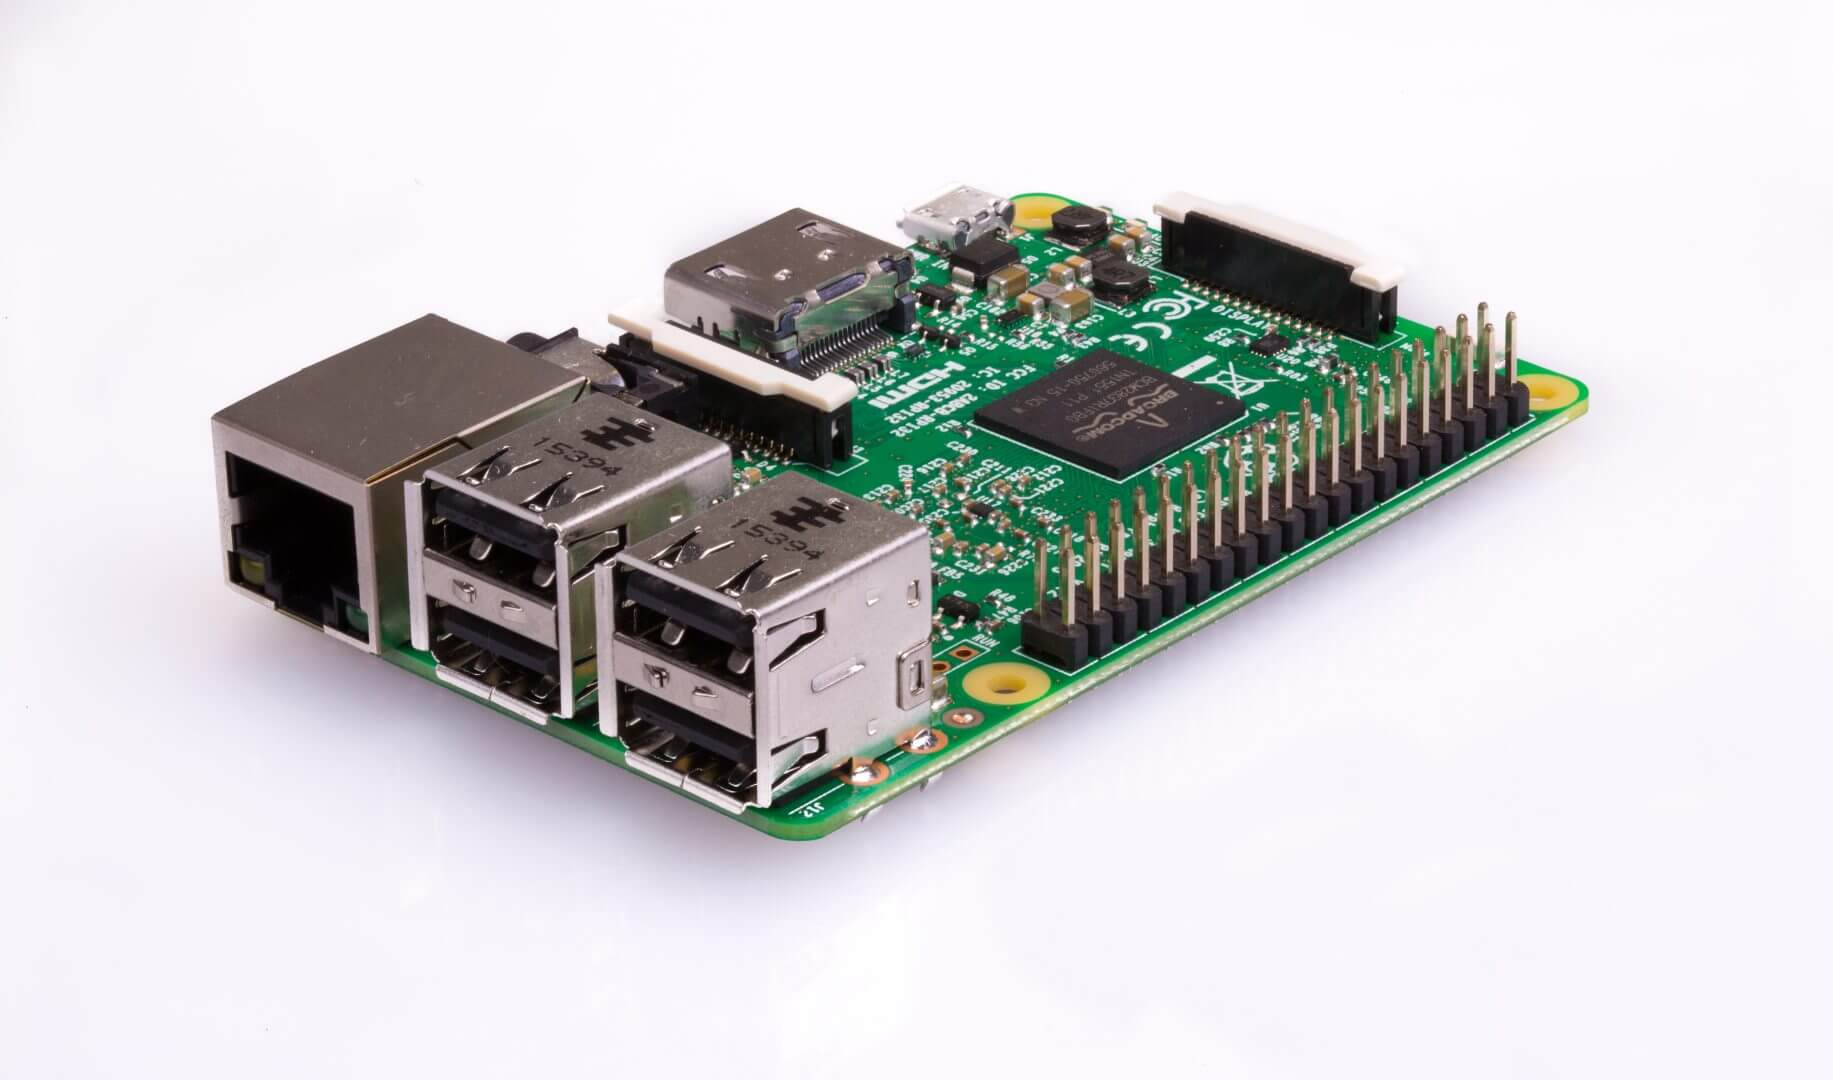
\includegraphics[width=0.6\linewidth]{Imagenes/raspberry3}
			\caption{Raspberry Pi 3}
			\label{fig:raspberry3}
		\end{figure}


	\subsection{Navio2}
		La placa Navio2 es un conjunto de sensores que se conectan sobre pines GPIO de una Raspberry Pi, transform�ndolo en un completo controlador de drones. Esta placa controladora suministra a la Raspberry Pi de sensores y entradas que son de suma importancia para cualquier tipo de veh�culo, con el objetivo de monitorear y obtener informaci�n para alg�n tipo de maniobra a�rea, como tambi�n terrestre.
		
		\begin{figure}[h!]
			\centering
			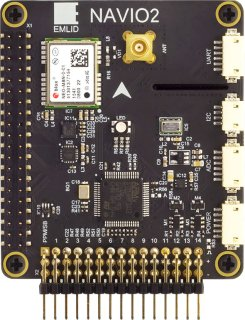
\includegraphics[width=0.4\linewidth, height=0.25\textheight]{Imagenes/navio22}
			\caption{Navio2}
			\label{fig:navio2}
		\end{figure}
		
		Dentro del conjunto de sensores que contiene esta placa tenemos:
		
	\subsubsection{IMU}
		Unidad de Medici�n Inercial (o por sus siglas en ingl�s \textit{Inertial Measurement Unit}) es el componente principal de los sistemas de navegaci�n. Son un conjunto de dispositivos electr�nicos, generalmente, una combinaci�n de aceler�metros, magnet�metros y giroscopios que miden e informan caracter�sticas del movimiento del veh�culo como pueden ser velocidad, fuerzas magn�ticas y orientaci�n. Como es un aspecto importante en este tipo de sistemas la precisi�n, la placa controladora Navio2 contiene dos de estas unidades con el fin de proporcionar y corroborar su informaci�n mediante dos fuentes de referencia distintas. Estas dos unidades son:
		
		\begin{enumerate}
			\item MPU9250 9DOF.
			\item LSM9DS1 9DOF.
			
		\end{enumerate}

	\subsubsection{GNSS}
		Obtener la posici�n del veh�culo mientras este se encuentra en movimiento es un aspecto sumamente necesario, m�s cuando la visibilidad del ambiente dificulta hacerlo, es por eso que el GNSS (\textit{Global Navigation Satellite System}) proporciona un posicionamiento geoespacial con cobertura global mediante un conjunto de tecnolog�as de sistemas de navegaci�n por sat�lite. Las tecnolog�as utilizadas en el m�dulo U-blox M8N de esta placa son:
		
		\begin{enumerate}
			\item Glonass.
			\item GPS.
			\item Beidou.
		\end{enumerate}


	\subsubsection{Entrada/Salida RC (Radio Control)} \label{sec:ioRC}
		La placa Navio2 tiene una entrada habilitada para recibir informaci�n proveniente del emisor mediante un radio control, aceptando se�ales por los protocolos de comunicaci�n PPM (Modulaci�n por Posici�n de Pulso) y SBUS �nicamente.
		

	\subsubsection{Bar�metro}
		El bar�metro tiene sus usos provenientes de la meteorolog�a para poder predecir el tiempo entre otras cosas, pero en este caso la placa controladora utiliza un bar�metro MS5611 de alta precisi�n (con 10cm de resoluci�n ) para poder estimar la altura en el cual se encuentra el dispositivo. 

	\subsubsection{Interfaces}
		\begin{itemize}
			\item Entrada UART (\textit{Universal Asynchronous Receiver-Transmitter})
			\item Bus de serie de datos $I^{2}C$ de sus siglas en ingl�s (Inter-Integrated Circuit)
			\item Conversor Anal�gico/Digital ADC
			\item Y por �ltimo. 14 salidas para servomotores mediante el protocolo PWM (Modulaci�n por Ancho de Pulso)
		\end{itemize}


	\subsection{Arduino UNO}
		El Arduino UNO es una plataforma computacional f�sica open-source basada en una simple tarjeta de I/O y un entorno de desarrollo que implementa el lenguaje Processing/Wiring. A diferencia de la Raspberry Pi 3, este est� fabricado para realizar tareas m�s sencillas, ya que su poder de procesamiento y memoria son limitados.
		\begin{itemize}
			\item Microcontrolador ATmega328.
			\item 14 pines digitales de I/O (6 salidas PWM).
			\item 6 entradas an�logas.
			\item 32KB de memoria Flash.
			\item Reloj de 16MHz de velocidad.	
		\end{itemize}
		\begin{figure}[h!]
			\centering
			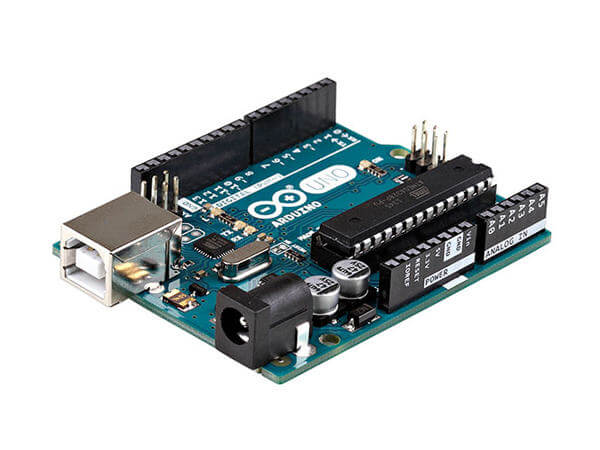
\includegraphics[width=0.5\linewidth, height=0.2\textheight]{Imagenes/arduinouno}
			\caption{Placa Arduino UNO}
			\label{fig:arduinouno}
		\end{figure}
		

	\subsection{Radio Control}
		Este control permite gobernar al veh�culo a distancia de manera inal�mbrica mediante se�ales de radio.
		\begin{figure}[h]
			\centering
			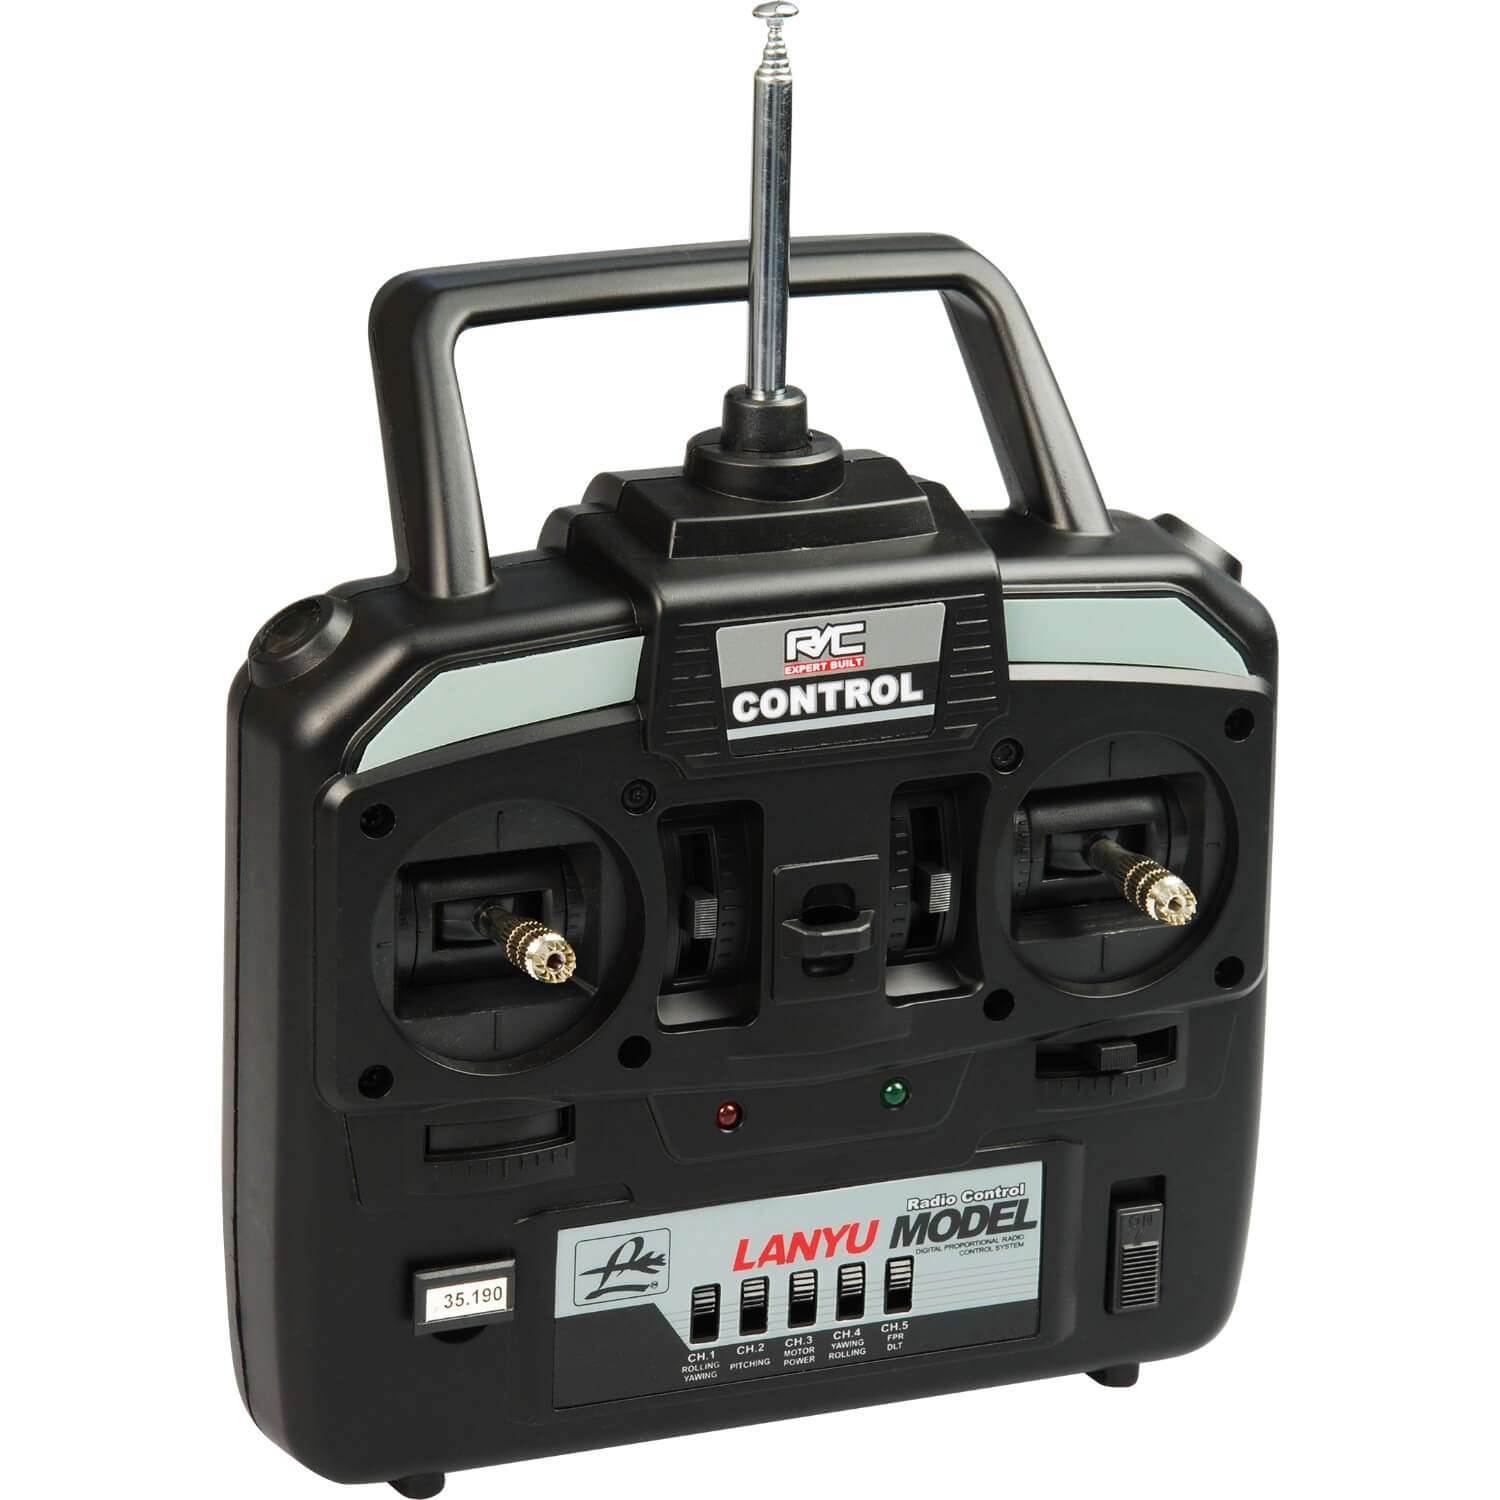
\includegraphics[width=0.4\linewidth, height=0.2\textheight]{Imagenes/RCcontrol}
			\caption{Comando Radio Control}
			\label{fig:rccontrol}
		\end{figure}



	\subsection{Joystick}	

		Una palanca de mando o com�nmente conocido como \textit{Joystick}  es un dispositivo que por lo general contiene 2 palancas con dos ejes cada uno, donde es posible representar la posici�n de un punto seg�n la posici�n f�sica de este y un conjunto de botones que al ser presionados y seg�n el software intermediario puede codificarse ciertas acciones. Este puede estar conectado mediante un cable USB o de manera inal�mbrica. En nuestro caso, utilizaremos un joystick con conexi�n USB ya que necesitamos que el env�o de informaci�n sea confiable.

	\subsection{Router}
	
		Un router es un dispositivo de hardware que permite la interconexi�n de ordenadores en red. El router o enrutador es un dispositivo que opera en capa de nivel de 3. As�, permite que varias redes u ordenadores se conecten entre s� y, por ejemplo, compartan una misma conexi�n de Internet. 
		\par Este dispositivo es usado para el desarrollo del proyecto ya que en el momento de las pruebas no se tienen a disposici�n los m�dulos de comunicaci�n verdaderos, estos m�dulos permiten una mayor distancia de cobertura y funciona exclusivamente para una conexi�n, lo que logra una mayor confiabilidad a la misma que comparando con el router que debe gestionar varias conexiones a la vez y la informaci�n enviada no est� asegurada. Por tal motivo de ausencia de estos m�dulos se recurre a utilizar como medio de comunicaci�n provisoria la tecnolog�a wifi del router, ya que �nicamente se pretende realizar pruebas en un �mbito controlado y de poca distancia.
	

	\subsection{M�dulos XBee}
	
		Los m�dulos XBee \footnote{P�gina web de XBee  https://www.digi.com/xbee} son soluciones integradas que brindan un medio inal�mbrico para la interconexi�n y comunicaci�n entre dispositivos. Estos m�dulos utilizan el protocolo de red llamado IEEE 802.15.4 para crear redes FAST POINT-TO-MULTIPOINT (punto a multipunto); o para redes PEER-TO-PEER (punto a punto). Est�n dise�ados para aplicaciones que requieren de un alto tr�fico de datos, baja latencia y una sincronizaci�n de comunicaci�n predecible.
	
		\begin{figure}[h!]
			\centering
			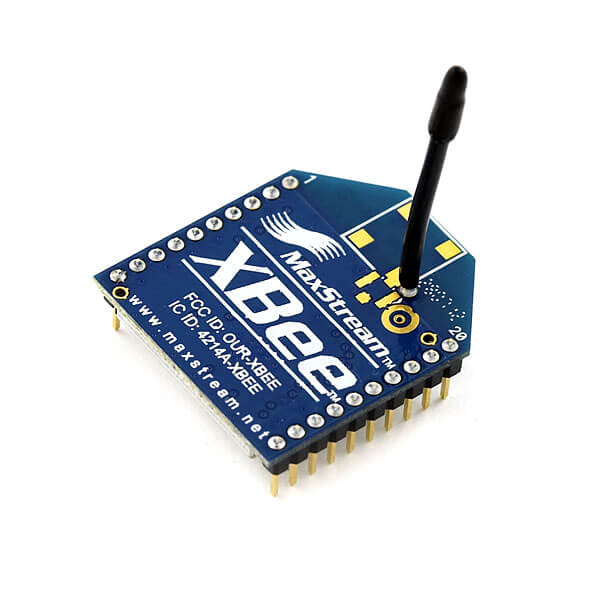
\includegraphics[width=0.4\linewidth, height=0.25\textheight]{Imagenes/xbee}
			\caption{M�dulo de comunicaci�n XBee}
			\label{fig:xbee}
		\end{figure}


	\subsection{Bater�a LiPo}
	
		La bater�a LiPo (Litio y Pol�mero) son bater�as recargables, compuestas generalmente de varias c�lulas conectadas en paralelo para aumentar la capacidad de la corriente de descarga. Esta contiene un voltaje de 12v con 2200 mA, suministrando dicha energ�a a los motores y adem�s a la Raspberry Pi con 5V.
		\begin{figure}[h!]
			\centering
			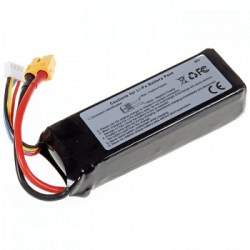
\includegraphics[width=0.2\linewidth, height=0.25\textheight]{Imagenes/bateria}
			\caption{Bater�a LiPo}
			\label{fig:bateria}
		\end{figure}
	


\section{Procedimiento}

	\subsection{Armado del cuerpo}
		Una vez ya descripto el hardware adquirido para el desarrollo de esta etapa,  estamos habilitados para iniciar el proceso del armado del veh�culo. En primera instancia se comienza con el cuerpo del cuadric�ptero, esta actividad  es realizada en base a las instrucciones que nos proporciona el vendedor \textit{ValueHobby} \footnote{http://www.valuehobby.com/media/wysiwyg/upload/Manual/bumblebee-manual.pdf} obteniendo el cuerpo armado como se puede observar en la Figura \ref{fig:armado}. Como medida de seguridad antes de realizar las pruebas se han extra�do las h�lices. Pero al momento se ser instaladas con el prop�sito de que el cuadric�ptero no se tumbe con respecto a su eje de orientaci�n cuando este se encuentre en el aire se deben colocar las h�lices pares de tal manera que su propulsi�n al momento de girar sea en sentido contra-horario y las h�lices impares deben estar colocadas en sentido horario tal como se ven en la Figura \ref{fig:esquemacuadricoptero} . 
		
		\begin{figure}[h!]
			\centering
			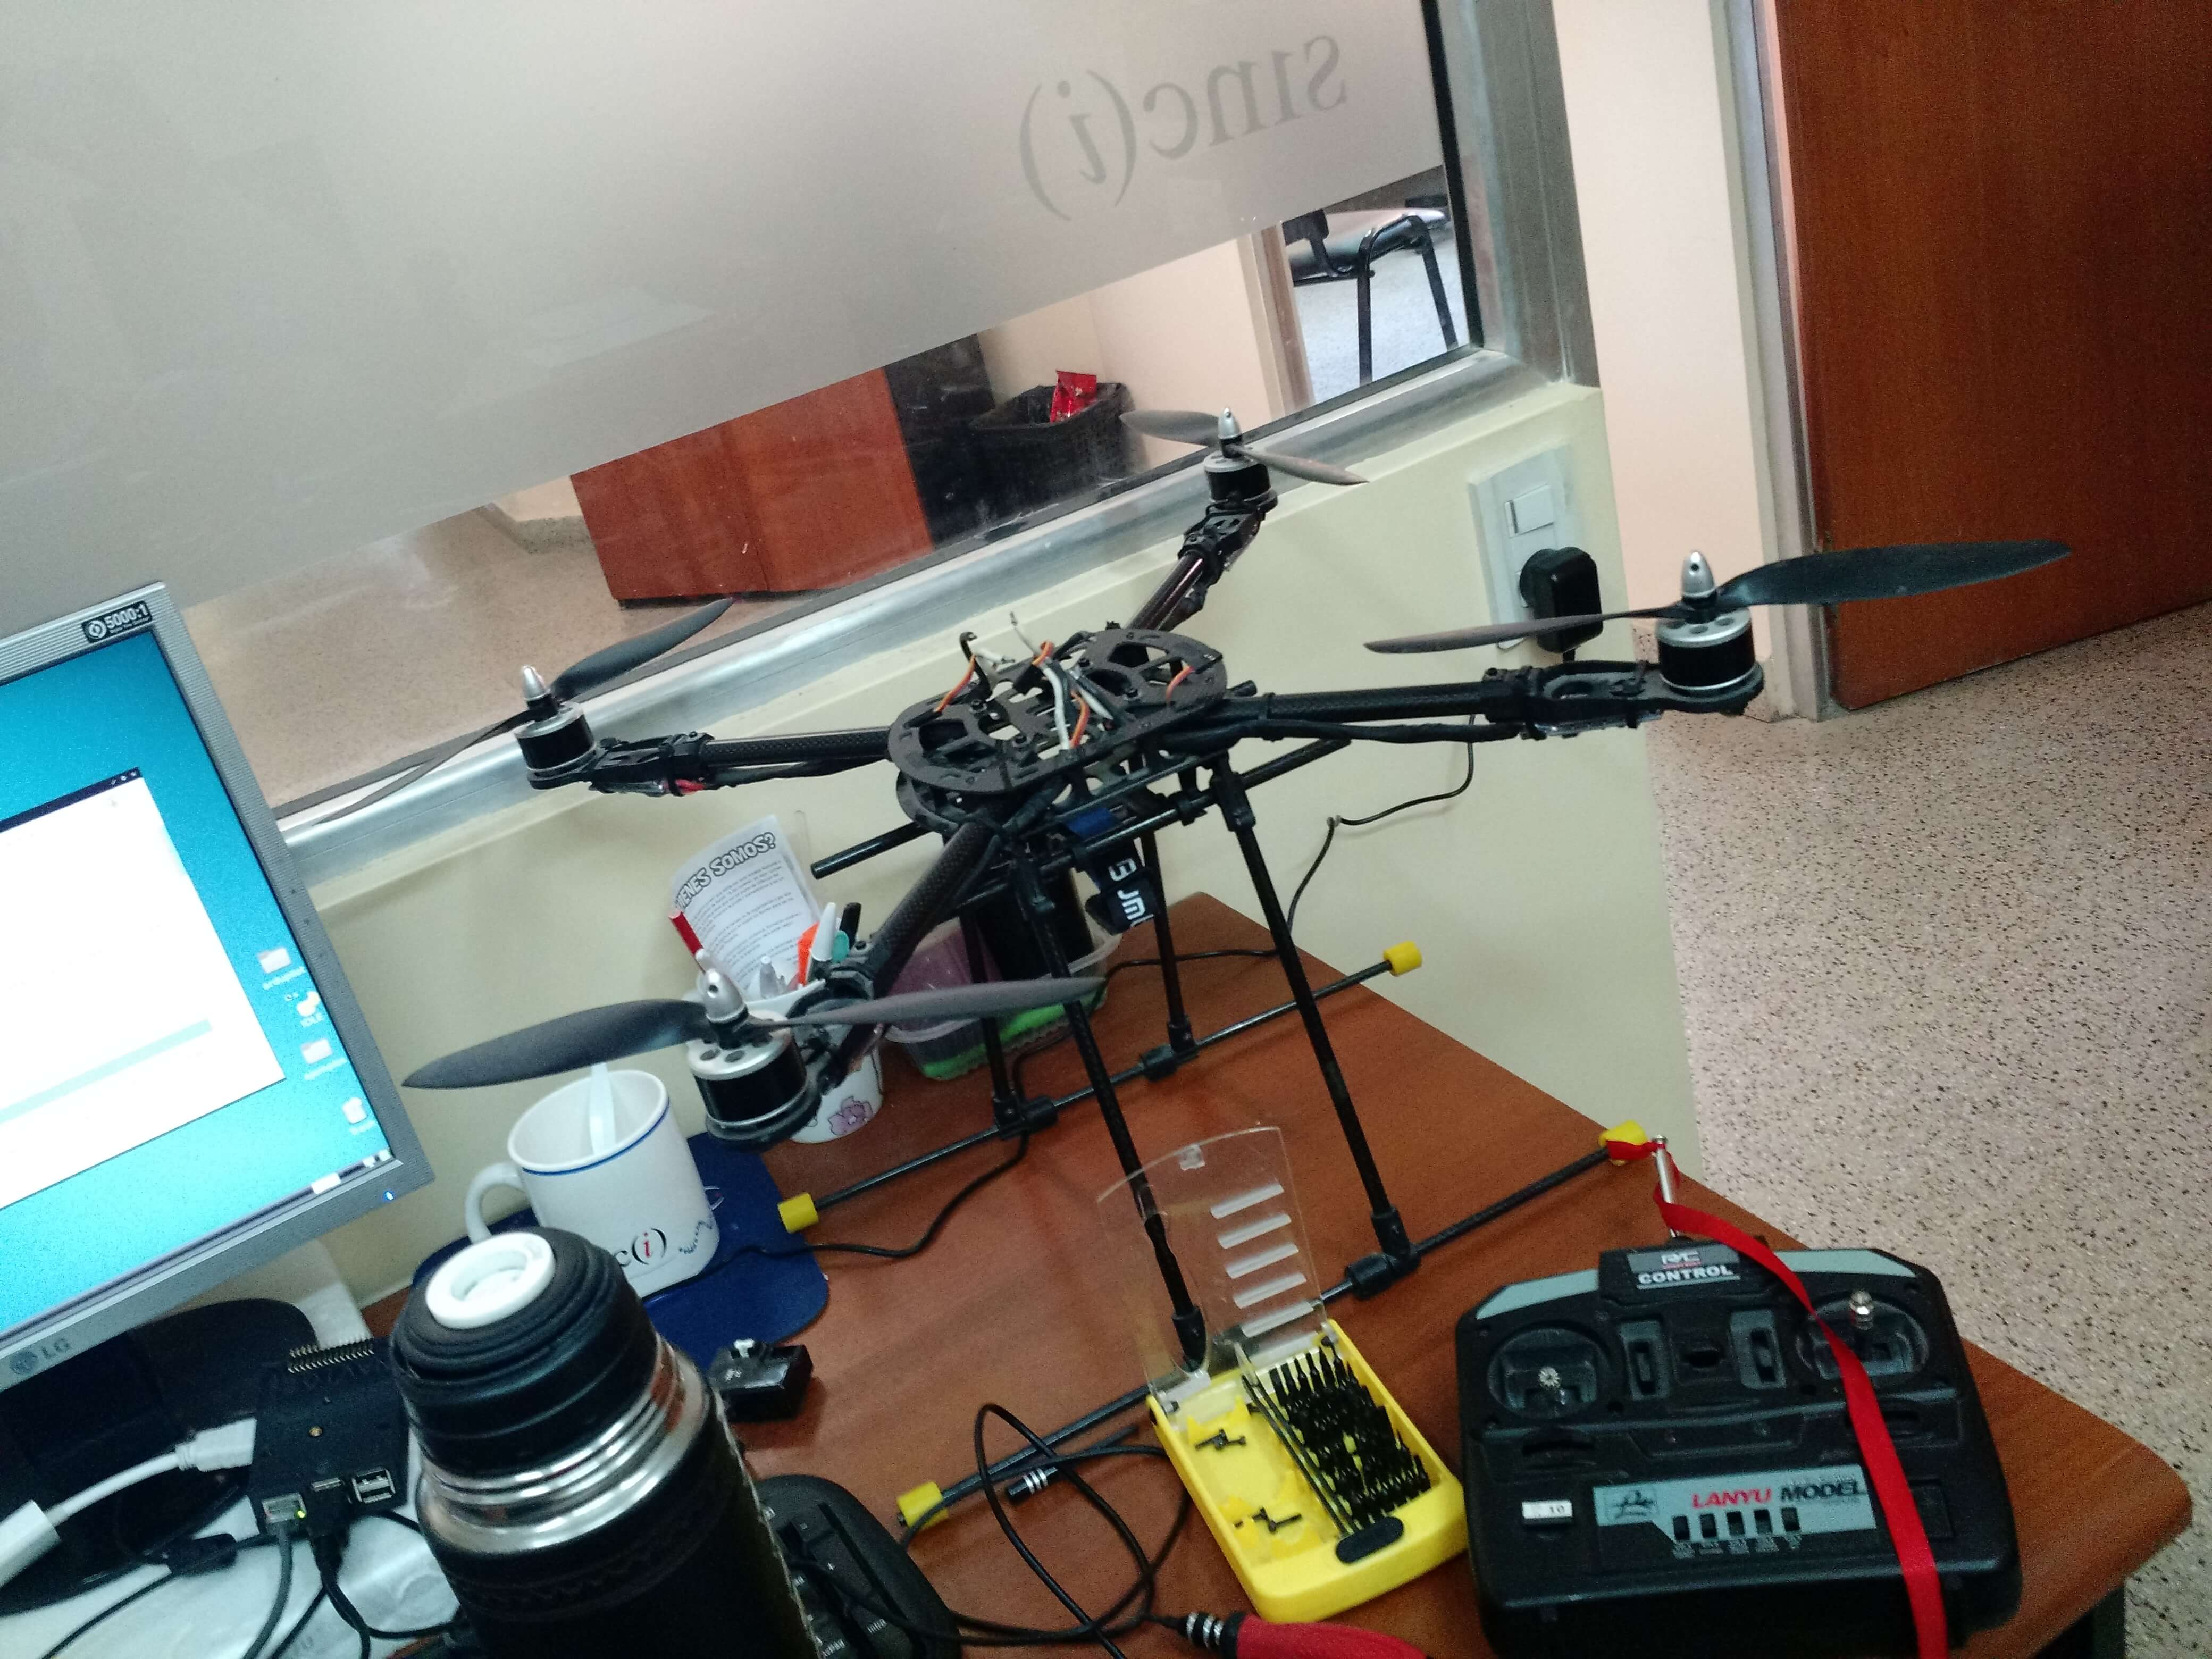
\includegraphics[width=0.6\linewidth, height=0.3\textheight]{Imagenes/fotos/Armado}
			\caption{Cuerpo de cuadric�ptero armado}
			\label{fig:armado}
		\end{figure}
		
		\begin{figure}[h!]
			\centering
			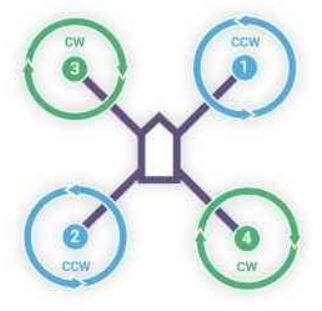
\includegraphics[width=0.3\linewidth, height=0.2\textheight]{Imagenes/esquemacuadricoptero}
			\caption{Esquema de instalaci�n de h�lices.}
			\label{fig:esquemacuadricoptero}
		\end{figure}

	\subsection{Armado y configuraci�n del piloto}
		En esta secci�n se describe el armado del piloto del cuadric�ptero, este va a ser el encargado en gestionar todos los sensores, enviar se�ales a los motores y administrar la informaci�n generada por estos sensores con el fin de ser enviadas a una maquina cliente y que este las pueda interpretar, entre otras cosas.
		
		
		\par Para comenzar con el armado debemos instalar la placa Navio2 sobre la Raspberry Pi 3, proporcionando as� los sensores indispensables para el control, monitoreo y vuelo del veh�culo ya que el ordenador de placa reducida Raspberry Pi no cuenta con estos sensores de forma nativa. Por lo tanto, se procede a conectar los 40 pines GPIO sobre la placa Navio2, como se muestra en la Figura \ref{fig:navio2-mount}
		
		
		\begin{figure}[h!]
			\centering
			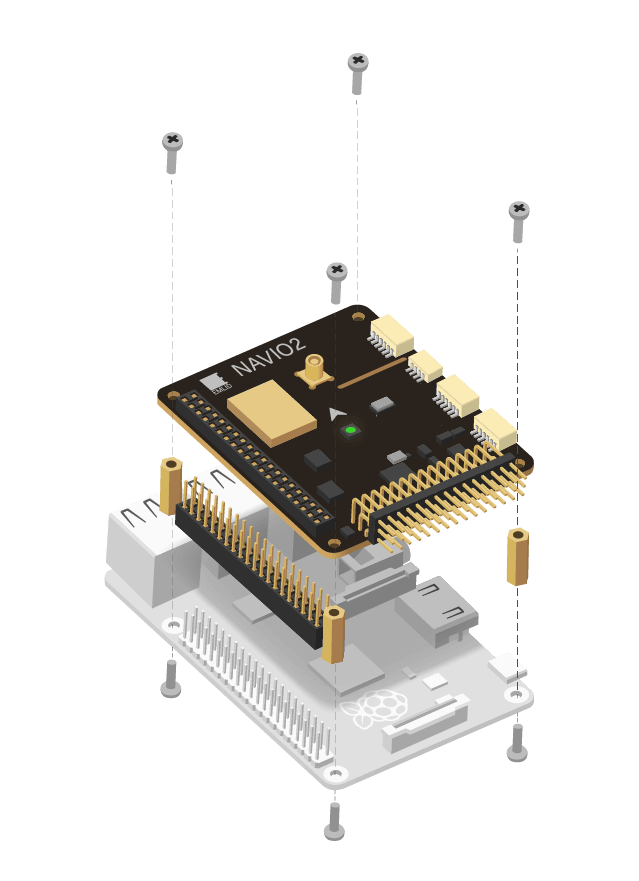
\includegraphics[width=0.4\linewidth, height=0.25\textheight]{Imagenes/navio2-mount}
			\caption{Conexi�n entre Raspberry Pi 3 y placa Navio2.}
			\label{fig:navio2-mount}
		\end{figure}
		
		Luego se procede a conectar la antena GNSS sobre la placa Navio2. Una vez ya conectado se debe verificar su correcto funcionamiento de todos los sensores presentes, para eso debemos tener un software que gestione eficazmente todo el hardware y sea el intermediario entre estos dispositivos electr�nicos y el usuario, adem�s de proporcionar servicios de utilidad para el mismo, en otras palabras, un sistema operativo (SO). Antes de instalar cualquier sistema operativo hay que tener en cuenta que  estamos en presencia de un ordenador de placa reducida, es decir, el hardware de los componentes del mismo como memoria, procesador, puertos de entrada y salida, etc�tera no son los mismos a los ordenadores comerciales que vemos com�nmente; por poner un ejemplo, el procesador que contiene la Raspberry es un ARM1176JZF-S, con esto queremos decir que el CPU en si mismo esta fabricado bajo una arquitectura con un conjunto reducido de instrucciones (o por su siglas en ingles \textit{RISC - Reduced instruction set computing}) en comparaci�n a un CPU que son utilizados normalmente en un ordenador hogare�o. Por tal motivo, es necesario de un SO que se adapte a estas caracter�sticas; afortunadamente existen varias organizaciones o empresas que desarrollan y distribuyen este tipo de producto, por ejemplo, \textit{Canonical Ltd} y \textit{Microsoft} han adaptado sus sistemas operativos para este tipo de ordenadores. En nuestro caso utilizaremos un SO proporcionado por la empresa \textit{Emlid} basado en una distribuci�n de Linux llamada \textit{Raspbian} (acr�nimo entre Raspberry Pi y Debian) donde ya viene preinstalado las herramientas necesarias.
		\par Una vez seleccionado el SO a instalar, se procede a descargar la imagen y grabarla en una tarjeta SD, una vez realizado este paso se carga la tarjeta SD en la ranura disponible en la Raspberry Pi, se enchufa un teclado, mouse y un conector HDMI que se encuentra conectado a un monitor, y por �ltimo se procede a encender el dispositivo  mostr�ndonos la siguiente imagen: 
		
		
		\begin{figure}[h!]
			\centering
			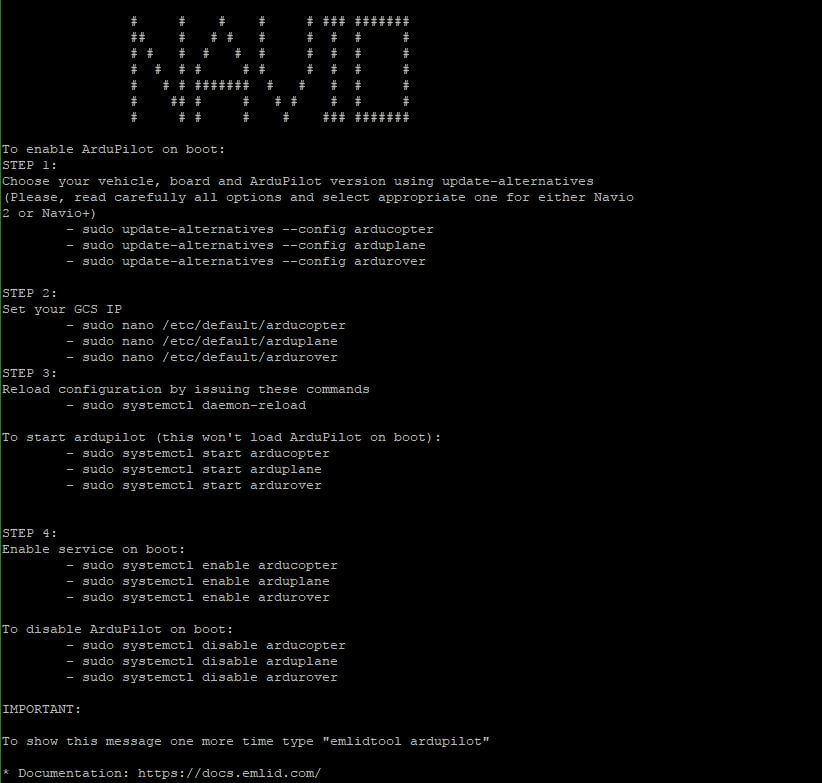
\includegraphics[width=0.8\linewidth, height=0.37\textheight]{Imagenes/pantallaInicio}
			\caption{Pantalla de bienvenida luego de instalar el SO}
			\label{fig:pantallainicio}
		\end{figure}
		
		Como se puede observar en la imagen \ref{fig:pantallainicio} la pantalla de bienvenida nos muestra los siguientes pasos que hay que seguir para configurar nuestro piloto.
		\begin{itemize}
			\item \textbf{Paso 1:} Se selecciona el tipo de veh�culo que se va a manejar, utilizando el comando \textit{update-alternatives}. Esta funci�n se encarga de seleccionar como predeterminada la opci�n ingresada dentro de otras alternativas, es decir, 
			Es posible que tenga en el sistema varios programas instalados a la vez  que  realizan  la
			misma  funci�n. Por ejemplo, muchos sistemas tienen varios editores de texto instalados al
			mismo tiempo, lo que deja la elecci�n de  qu�  editor  de  texto  utilizar  en  manos  del
			usuario,  si  �ste lo desea, pero hace dif�cil que un programa elija la opci�n correcta si
			el usuario no ha definido ninguna preferencia. En nuestro caso es el tipo de autopiloto como puede ser arducopter, arduplaner y ardurover. Como estamos por utilizar un cuadric�ptero ingresamos:
			
			\begin{listing}[style=consola, numbers=none]
				> sudo update-alternatives --config arducopter
			\end{listing}
				
				
				
				\item \textbf{Paso 2:} Se debe ingresar dentro del archivo /etc/default/arducopter el IP perteneciente al GCS (\textit{Ground Control Station}), es decir, este archivo contiene la direcci�n IP del ordenador que enviar� y recibir� informaci�n del veh�culo. Adem�s, brinda la opci�n de seleccionar la interfaz por el que se realizar� la comunicaci�n. En nuestro caso lo haremos realizaremos mediante tecnolog�a Wifi y utilizando el protocolo UDP \footnote{Es posible tambi�n utilizar el protocolo TCP, pero la raz�n por la cual se este m�todo es porque es un protocolo no orientado a la conexi�n, por lo tanto como estaremos realizando maniobras que son ejecutadas por el veh�culo en tiempo real necesitamos la menor latencia posible y no estar esperando paquetes de confirmaci�n todo el tiempo}. 
				
				\item \textbf{Paso 3:} Una vez ya seleccionado el tipo de veh�culo a utilizar e ingresado el IP de nuestro GCS se debe iniciar los servicios y procesos proporcionados por arducopter (ya que este se encargar� de administrar las funcionalidades pertinentes), para eso se utiliza el gestor del sistema y servicios \textbf{systemd} de Linux con el objetivo de iniciar un conjunto nuevo de procesos y servicios encapsulados en Arducopter, para eso utilizamos los siguiente comandos :
				
				\begin{listing}[style=consola, numbers=none]
				> sudo systemctl daemon-reload
				> sudo systemctl start arducopter 
				\end{listing}
				
				
				
				
				\item \textbf{Paso 4:} Por �ltimo es deseable que los servicios proporcionados por Arducopter se inicien cada vez que el veh�culo se encienda, por tal motivo se ingresa el �tlimo comando :
				
				\begin{listing}[style=consola, numbers=none]
				> sudo systemctl enable arducopter 
				\end{listing}
			
			
			
		\end{itemize}

	\subsection{Configuraci�n para el acceso a la red}

		\par Entre las opciones de conexi�n a la red que dispone la Raspberry Pi 3, podemos identificar que el mismo tiene una entrada Ethernet como tambi�n un m�dulo interno Wi-Fi, por lo tanto es necesario configurar dichas interfaces para poder conectarnos mediante un cable UTP con un conector RJ45, como tambi�n por tecnolog�a \textit{Wireles}. Por lo que dentro del sistema operativo del veh�culo y sobre la consola se ingresa el siguiente comando 
		\begin{listing}[style=consola, numbers=none]
			> sudo ifconfig
		\end{listing}
		Con este comando podemos verificar nombres de interfaces presentes y si se encuentran en actual funcionamiento. En caso de observar ning�n tipo de trafico por estas interfaces se procede a configurarlas, para esto se utiliza el mismo comando pero con la opci�n de activar la interfaz deseada, en nuestro caso queremos activar la interfaz del m�dulo interno de Wi-Fi, para eso ingresamos el siguiente comando 
		\begin{listing}[style=consola, numbers=none]
		> sudo ifconfig intwifi0 up
		\end{listing}
		Una vez ya activo podemos buscar las redes disponibles y que son captadas por el m�dulo, utilizando el siguiente comando 
		
		\begin{listing}[style=consola, numbers=none]
			> iwlist wlan0 scan
			\end{listing}
			Con este comando nos muestra mediante una lista las redes captadas por el m�dulo, una vez que hayamos encontrado la red de nuestro inter�s podemos conectarnos con el siguiente comando 
			
			\begin{listing}[style=consola, numbers=none]
			> iwconfig wlan0 essid "Nombre de Red" key "Contrasena"
		\end{listing}
		y finalmente procederemos a obtener nuestra IP y conectarnos con la siguiente funci�n :

		\begin{listing}[style=consola, numbers=none]
		> sudo dhclient wlan0
		\end{listing}
		
		En caso de querer almacenar esta red e indicarle al sistema operativo que es nuestra red por defecto podemos modificar el archivo wpa\_supplicant.conf ingresando el nombre de la red y su correspondiente clave.
		Por �ltimo, se reinicia y una vez iniciado el sistema se comprueba su conectividad realizando chequeo de conexi�n con alg�n tipo de p�gina en internet, por ejemplo, Google utilizando el siguiente comando 
		\begin{listing}[style=consola, numbers=none]
		> ping 8.8.8.8
		\end{listing}


	\subsection{Instalaci�n del firmware}

		\par Una vez ya comprobado la conectividad a la red y conFigurado el sistema operativo, es necesario instalar el \textit{firmware}  encargado de gestionar todos los sensores que se han incluido a la Raspberry mediante la placa Navio2, con el objetivo de poder administrar esta informaci�n y poder enviarla al \textit{GCS}. Para instalar el firmware se procede a descargarlo desde el mismo SO del veh�culo mediante el siguiente comando 
		
		
		\begin{listing}[style=consola, numbers=none]
			
			pi@navio: ~\$ wget http://firmware.eu.ardupilot.org/Copter/stable/navio2-quad/arducopter-quad
			pi@navio: ~\$ chmod +x arducopter-quad}
		
		\end{listing}
		
		Una vez descargado el firmware se desea que los servicios ya instalados de Arducopter utilicen dicho firmware actualizado, por lo tanto se procede a modificar el archivo /etc/systemd/system/ardupilot.service. Modificando la l�nea  
		
		\begin{listing}[style=consola, numbers=none]
		#ExecStart=/bin/sh -c "/home/pi/path/to/your/binary \$\{ARDUPILOT\_OPTS\}"
		\end{listing}
		por
		\begin{listing}[style=consola, numbers=none]
		#ExecStart=/bin/sh -c "/home/pi/arducopter-quad \$\{ARDUPILOT\_OPTS\}"}
		\end{listing}


	\subsection{Primeras pruebas}	\label{sec:primprue}
		Ya instalado el firmware correspondiente dentro de la Raspberry Pi estamos en condiciones de poder hacer nuestras primeras pruebas, para eso, dentro del mismo veh�culo se ejecutan programas proporcionados por ArduPilot para poder observar los datos generados por los sensores. En la misma carpeta de instalaci�n se encuentran programas de ejemplo para observar los datos provenientes de los sensores y al ejecutar dichos programas evidentemente la informaci�n mostrada es err�nea ya que estos sensores no se encuentran calibrados, por lo tanto, para realizar estas correcciones utilizamos las herramientas recomendadas y proporcionadas por la empresa ArduPilot como es el software \textbf{MavProxy} (Figura \ref{fig:mavproxy}), este software muestra a trav�s de una consola todos los datos obtenidos de los sensores, estado del veh�culo entre otras cosas, siendo lo m�s importante poder calibrar los sensores.
		\begin{figure}[h]
		\centering
		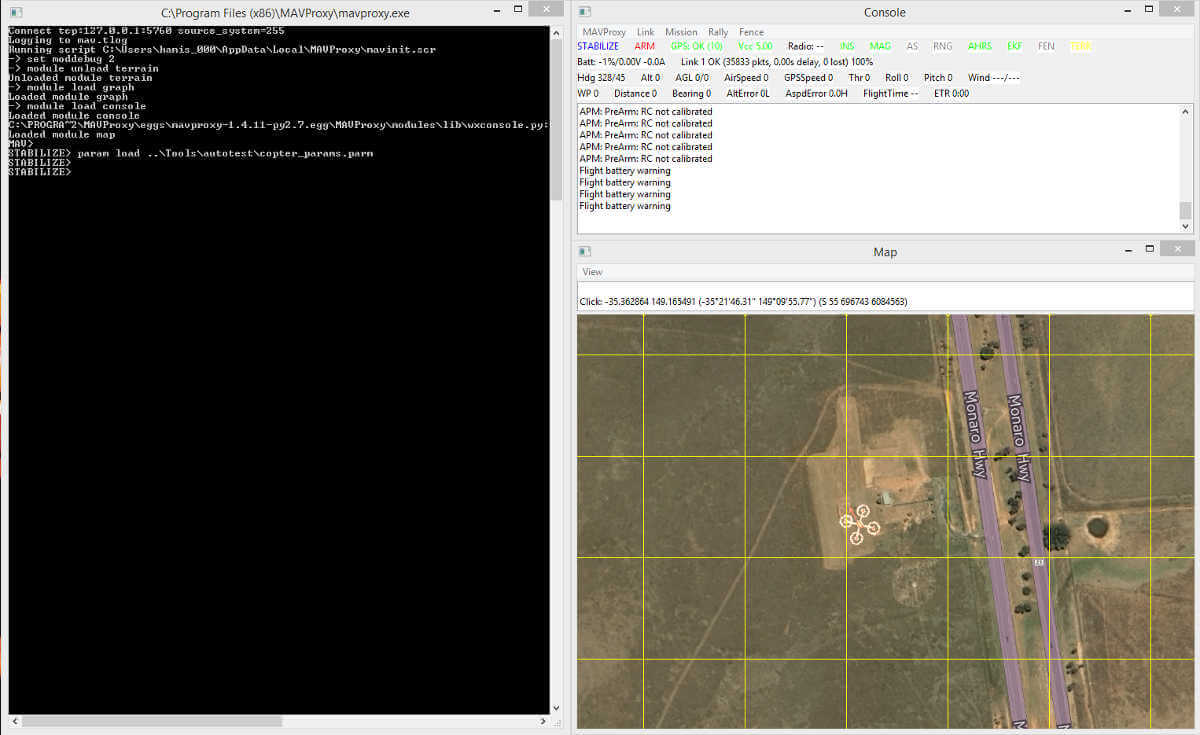
\includegraphics[width=0.8\linewidth, height=0.4\textheight]{Imagenes/mavproxy}
		\caption{Captura de pantalla del Software MavProxy}
		\label{fig:mavproxy}
		\end{figure} 
		As� que una vez iniciado el software se prueba la opci�n de calibrarlos. Al momento de iniciar el proceso de calibraci�n surge el inconveniente de no poder iniciarlo, ya que para realizar dicha acci�n es de suma importancia tener conectado el radio control al veh�culo. Esto genera un inconveniente al momento del desarrollo de esta fase ya que la compra de un radio control conllevar�a un tiempo extra en el cronograma del proyecto. Buscando alternativas en conjunto se descubre que es posible realizar la calibraci�n mediante un script que deb�amos codificar. Analizando esta propuesta se descubre que para generar dicho script es necesario de estudiar las librer�as involucradas lo que conlleva un tiempo considerado y �nicamente el objetivo de esta fase es realizar la comprobaci�n funcional de estos dispositivos. De esta manera se obtiene provisoriamente un radio control como se ilustra en la imagen \ref{fig:radiocontrol}
		
		\begin{figure}[h!]
		\centering
		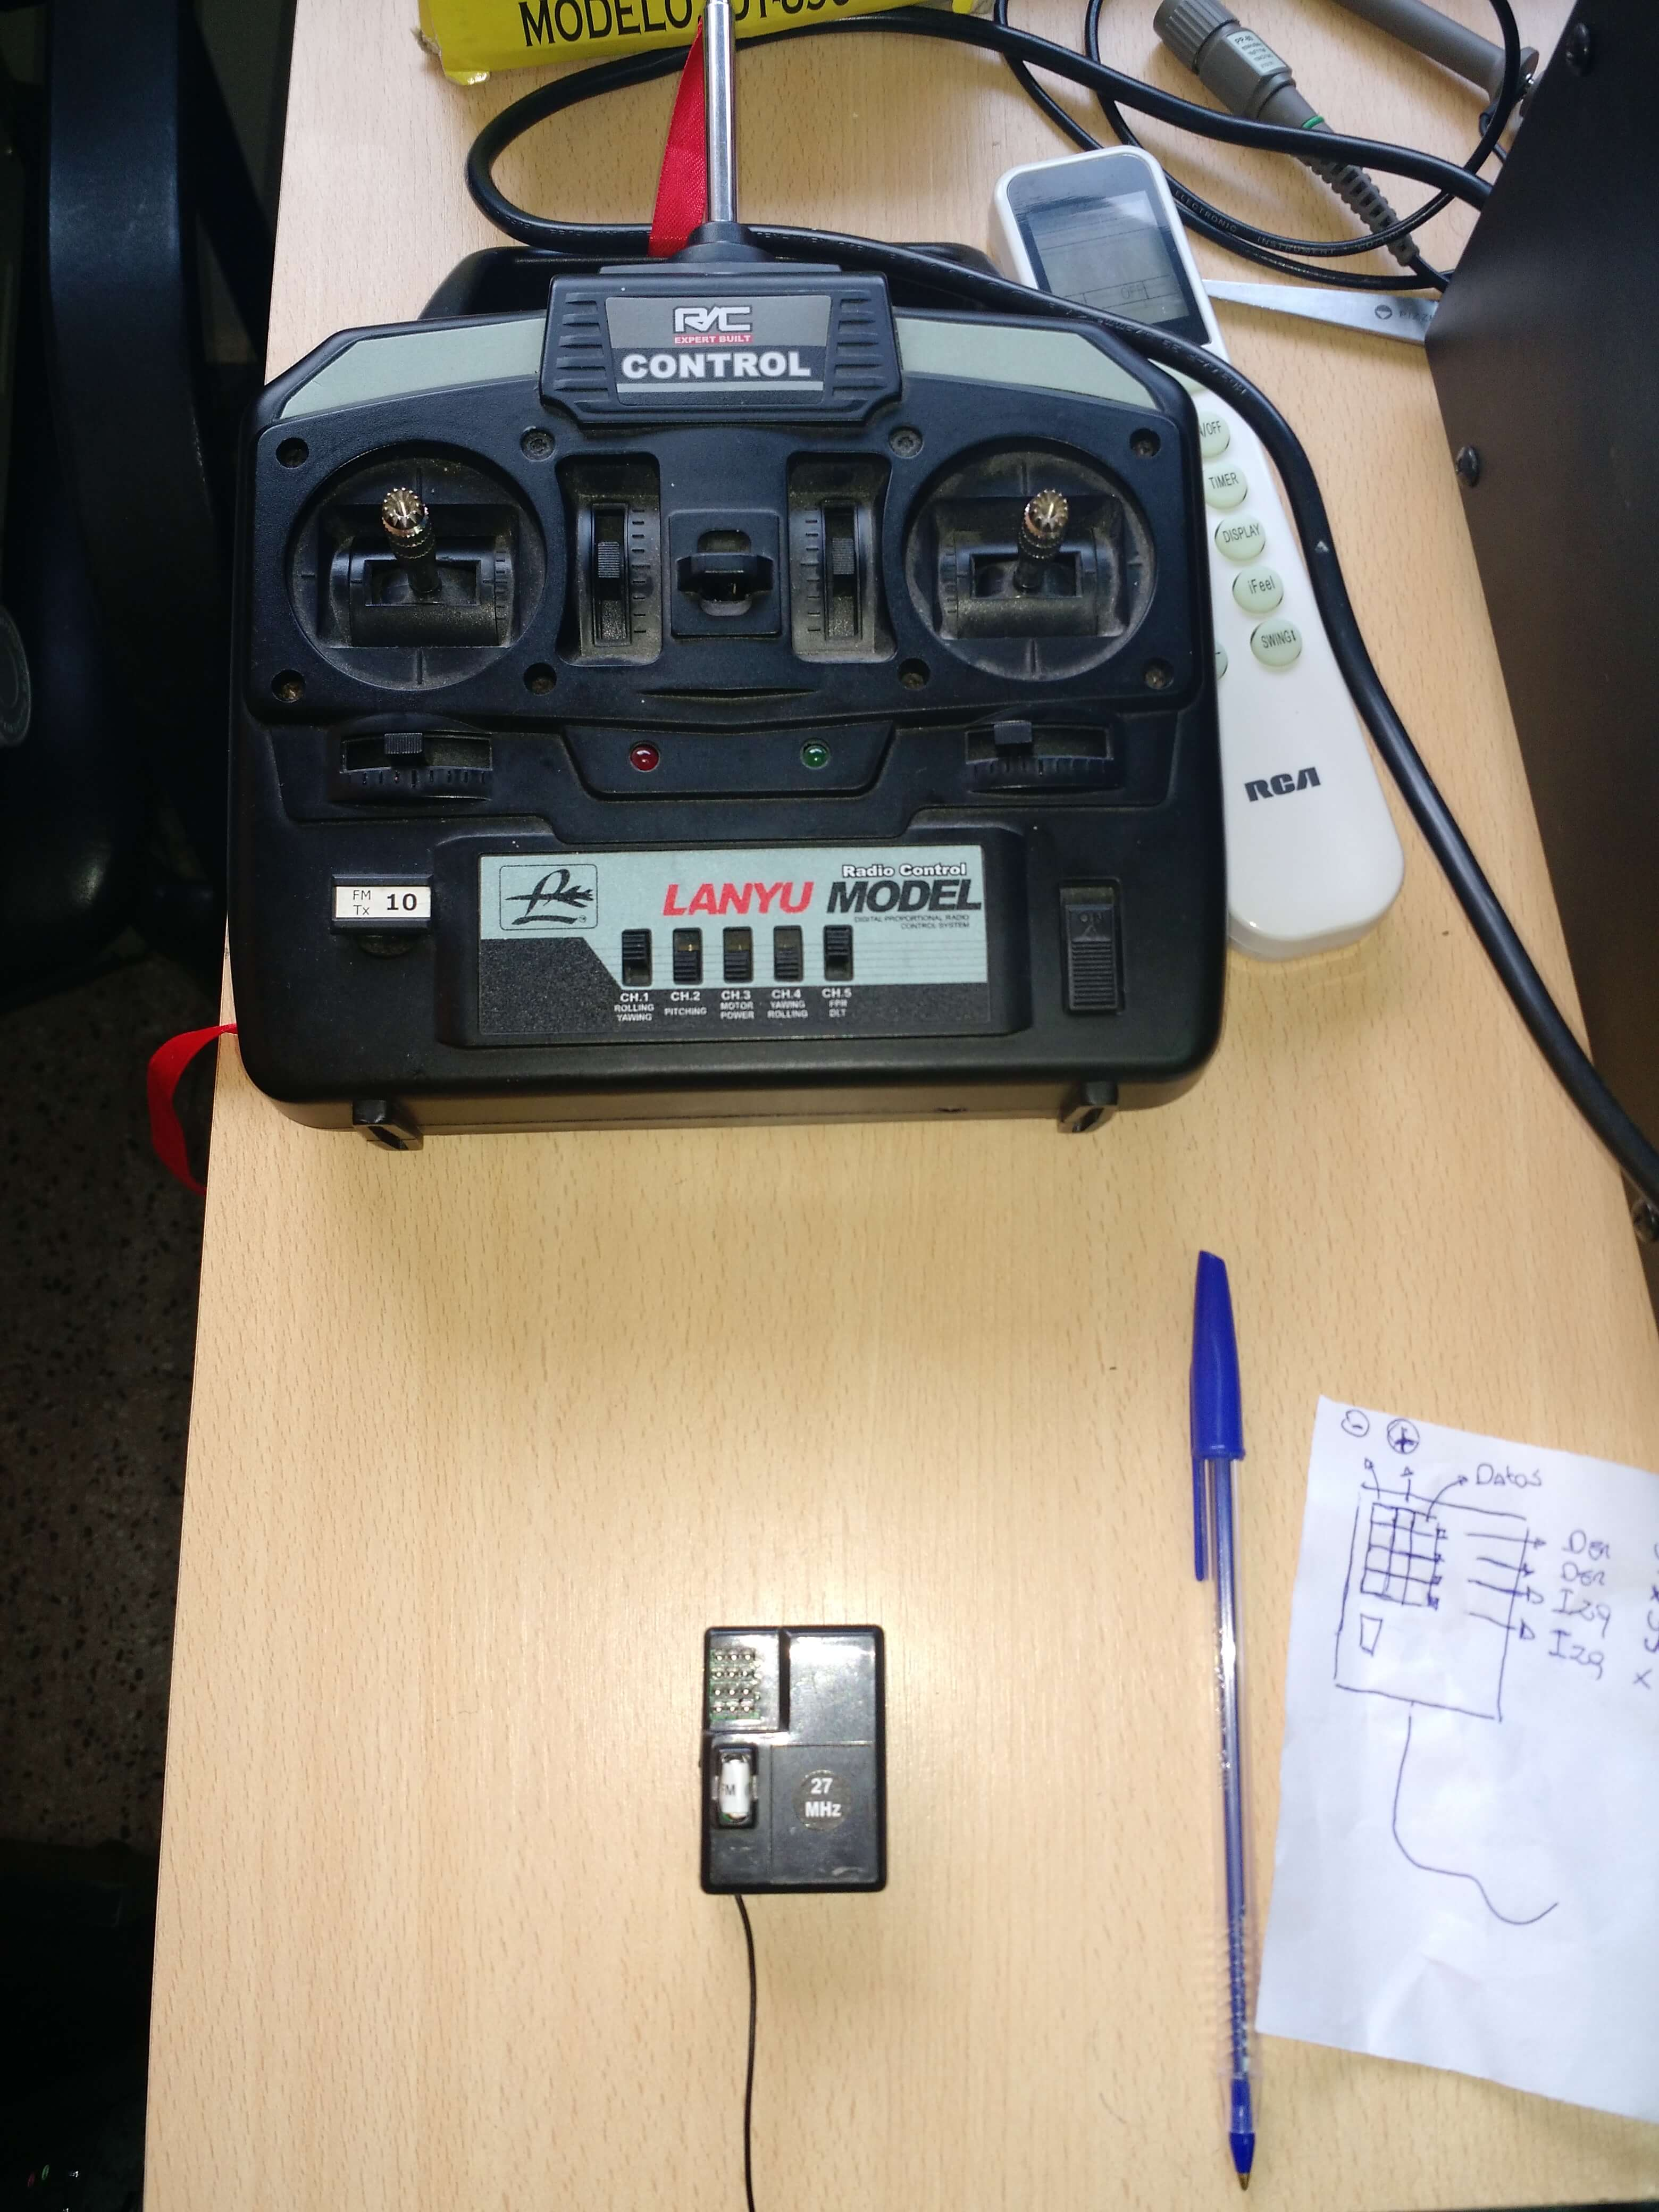
\includegraphics[width=0.5\linewidth, height=0.5\textheight]{Imagenes/fotos/rc_control_receptor}
		\caption{Radio Control LANYU model y su correspondiente receptor.}
		\label{fig:radiocontrol}
		\end{figure}
		
		Este radio control simplemente env�a las se�ales por 4 canales independientes, que son generados por sus dos palancas donde cada una contiene 2 ejes (\textit{eje x y eje y}), por lo tanto tendr�amos que la palanca 1 enviar� informaci�n del $eje_{p1} x$ y $eje_{p1} y$ y de la misma manera, la palanca 2 enviar� informaci�n de el $eje_{p2} x$ y $eje_{p2} y$ mediante la t�cnica de modulaci�n por ancho de pulso. Simplificando un poco, el receptor o (\textit{RX})  tendr� 4 cables con informaci�n de cada canal y que deber� conectarse al veh�culo, pero recordando la secci�n \ref{sec:ioRC} el veh�culo solo dispone de una entrada compatible con PPM o SBUS. Por lo que aqu� surge otro problema, debemos encontrar la forma de poder convertir las se�ales del radio control que se encontraban en PWM y pasarlas a PPM o SBUS para que el veh�culo pueda interpretar esta informaci�n. Para solucionar este problema se plantean 3 alternativas:
		
		\begin{enumerate}
		\item \textbf{Comprar un radio control con su respectivo receptor compatible con el veh�culo.}   
		\item \textbf{Realizar manualmente un conversor de PWM a PPM o SBUS con componentes electr�nicos desde cero. }   
		\item \textbf{Implementar el conversor sobre una placa Arduino UNO.}   
		\end{enumerate}
		
		Para estas propuestas se realiza el siguiente an�lisis:\newline
		\par \textbf{Propuesta 1: } La adquisici�n de un nuevo radio control m�s all� de sus futuros usos conllevar�a un elevado costo adicional para el proyecto ya que el mismo tiene un valor de \$8000 \footnote{Fecha consultada, septiembre del 2017}, adem�s atrasar�a el cronograma los d�as que se deban esperar el producto desde su ciudad de origen.
		
		\par \textbf{Propuesta 2: } Consiste en realizar la compra de los componentes electr�nicos de tipo CMOS CD4001 \footnote{http://www.alldatasheet.es/datasheet-pdf/pdf/26834/TI/CD4001.html} y 	CD40106 \footnote{http://www.alldatasheet.es/datasheet-pdf/pdf/26839/TI/CD40106.html} con un precio estimado de \$100. A pesar de su bajo costo de implementaci�n y siendo la mano de obra realizada por el profesor de la c�tedra Electr�nica Digital, es una tarea ajena al ejecutante del proyecto, por lo que no complementar�a los conocimientos del alumno.
		
		\par \textbf{Propuesta 3: } Esta propuesta consiste en implementar la funci�n de conversi�n de PWM a PPM o SBUS mediante un script que se implementar� sobra la placa Arduino, donde se conectar�n los cables provenientes del Rx a sus entradas y retornar� en una de sus salidas un �nico cable con la informaci�n codificada en PPM o SBUS como estaba especificado en el sitio web del fabricante. El precio estimado de la placa Arduino UNO es de \$200, pero existen versiones reducidas como el Arduino Nano que cuentan con un precio a la mitad del Arduino UNO. De manera conveniente se contaba con la adquisici�n de un Arduino UNO, por lo que no hacia falta realizar una compra. Adem�s, la implementaci�n de este algoritmo contribuye al crecimiento de las aptitudes del ejecutante del proyecto como estudiante de ingenier�a en inform�tica. 
		% TODO: Explicar codificaci�n del script	 
		Por lo que finalmente se decide realizar la propuesta 3. Una vez realizada se implementa sobre la placa Arduino UNO y se comprueban los resultados con un osciloscopio, d�ndonos un resultado favorable.




	\subsection{Conexi�n de componentes}
		
		Antes de comenzar a describir el proceso de cableado del veh�culo se comienza conectando el receptor del comando radio control con el Arduino UNO que va a ser el en cargado de recibir las se�ales PWM y convertirlas en SBUS moment�neamente para poder enviarlas a la Navio2. Hay que tener en cuenta que la ubicaci�n de los conectores y los pines del receptor llevan un orden en espec�fico. Por tal motivo, se investiga dicho orden, pero sin encontrar informaci�n relevante, hasta ubicar con un transmisor de la misma empresa y deducir las siguientes conexiones
		
		
		\begin{figure}[h!]
		\centering
		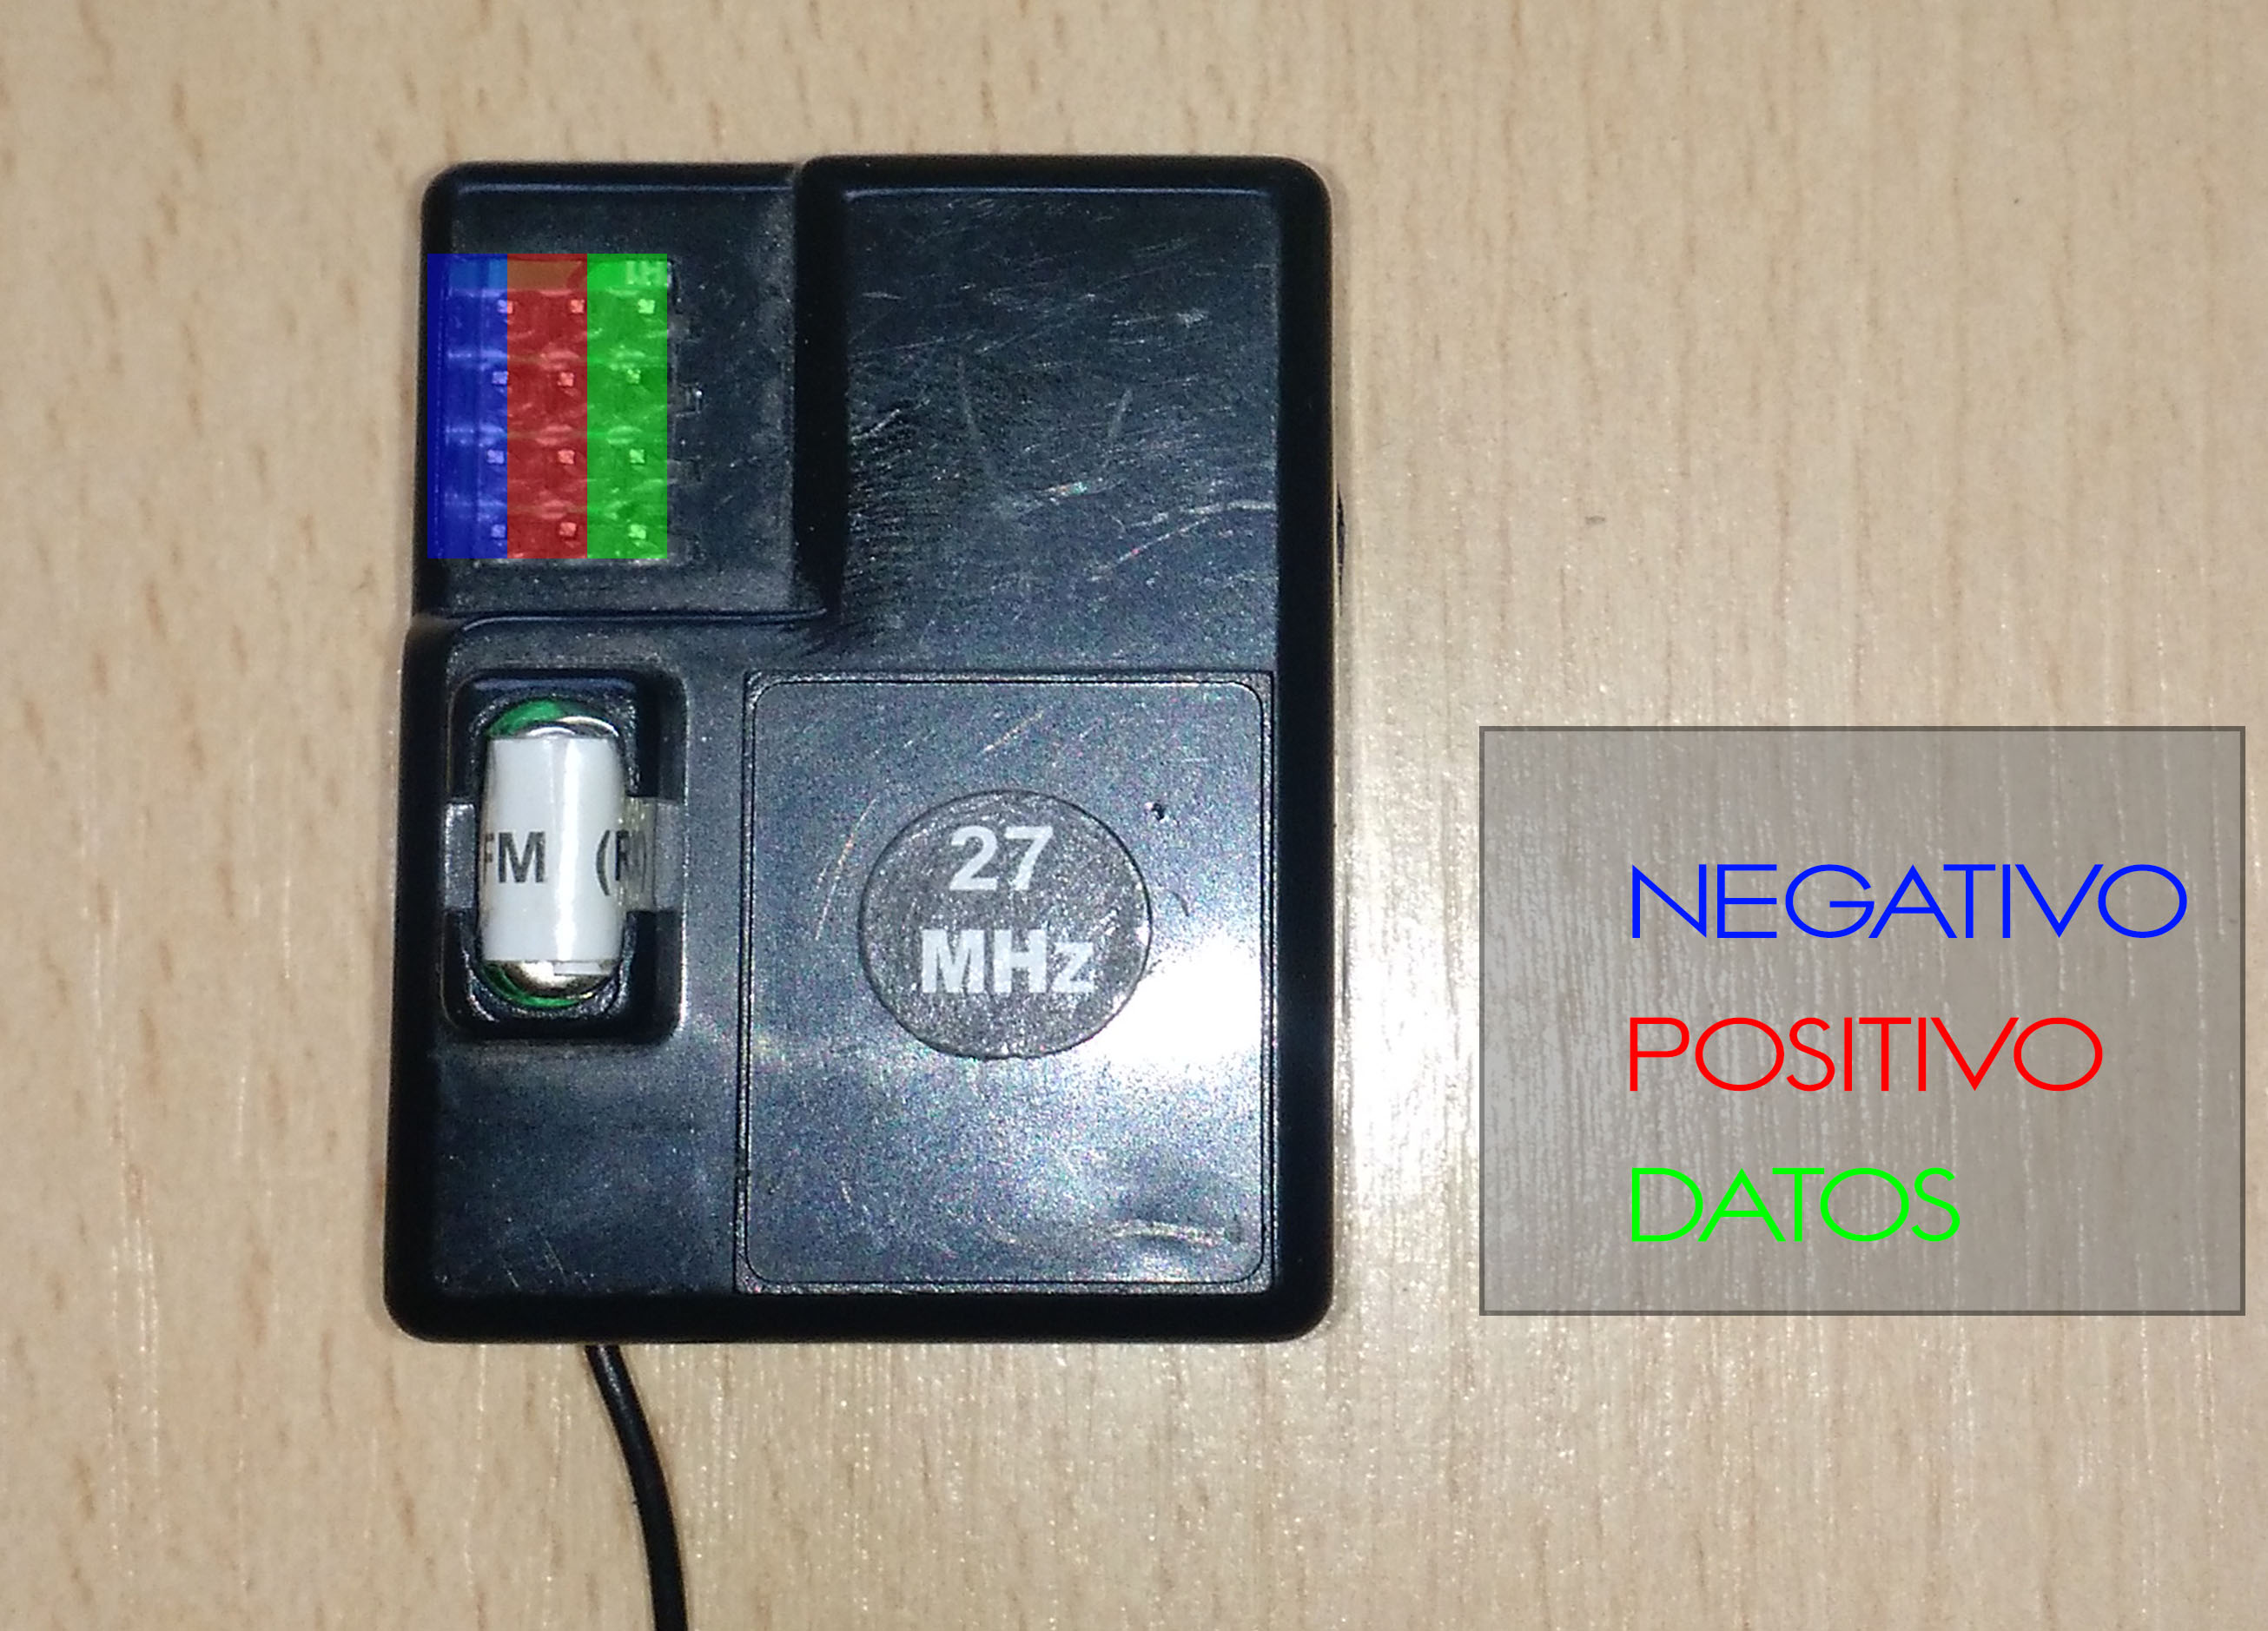
\includegraphics[width=0.5\linewidth, height=0.3\textheight]{Imagenes/fotos/Rxconexion}
		\caption{Ubicaci�n de conexiones en el Rx}
		\label{fig:RxConexiones}
		\end{figure}
		
		Como se puede observar en la Figura \ref{fig:RxConexiones} la columna izquierda de pines le pertenece a los negativos, la columna central a los positivos y la �ltima columna perteneciente a datos; esta es la de inter�s ya que por cada $conector_i$ estar�amos recibiendo se�al PWM del emisor correspondiente al $canal_i$, por lo que cada una son las entradas a nuestro Arduino UNO para poder realizar la codificaci�n. Antes de iniciar la conexi�n con el codificador se comprueban las se�ales mediante un osciloscopio. 
		\par Ya identificados los cables correspondientes a cada canal, se conectan los mismos a la placa Arduino UNO. Por �ltimo, se conecta la salida proporcionada por el codificador a la entrada del veh�culo, asegurando as� una se�al de tipo SBUS como lo indica su fabricante.
		
		\begin{figure}[h!]
		\centering
		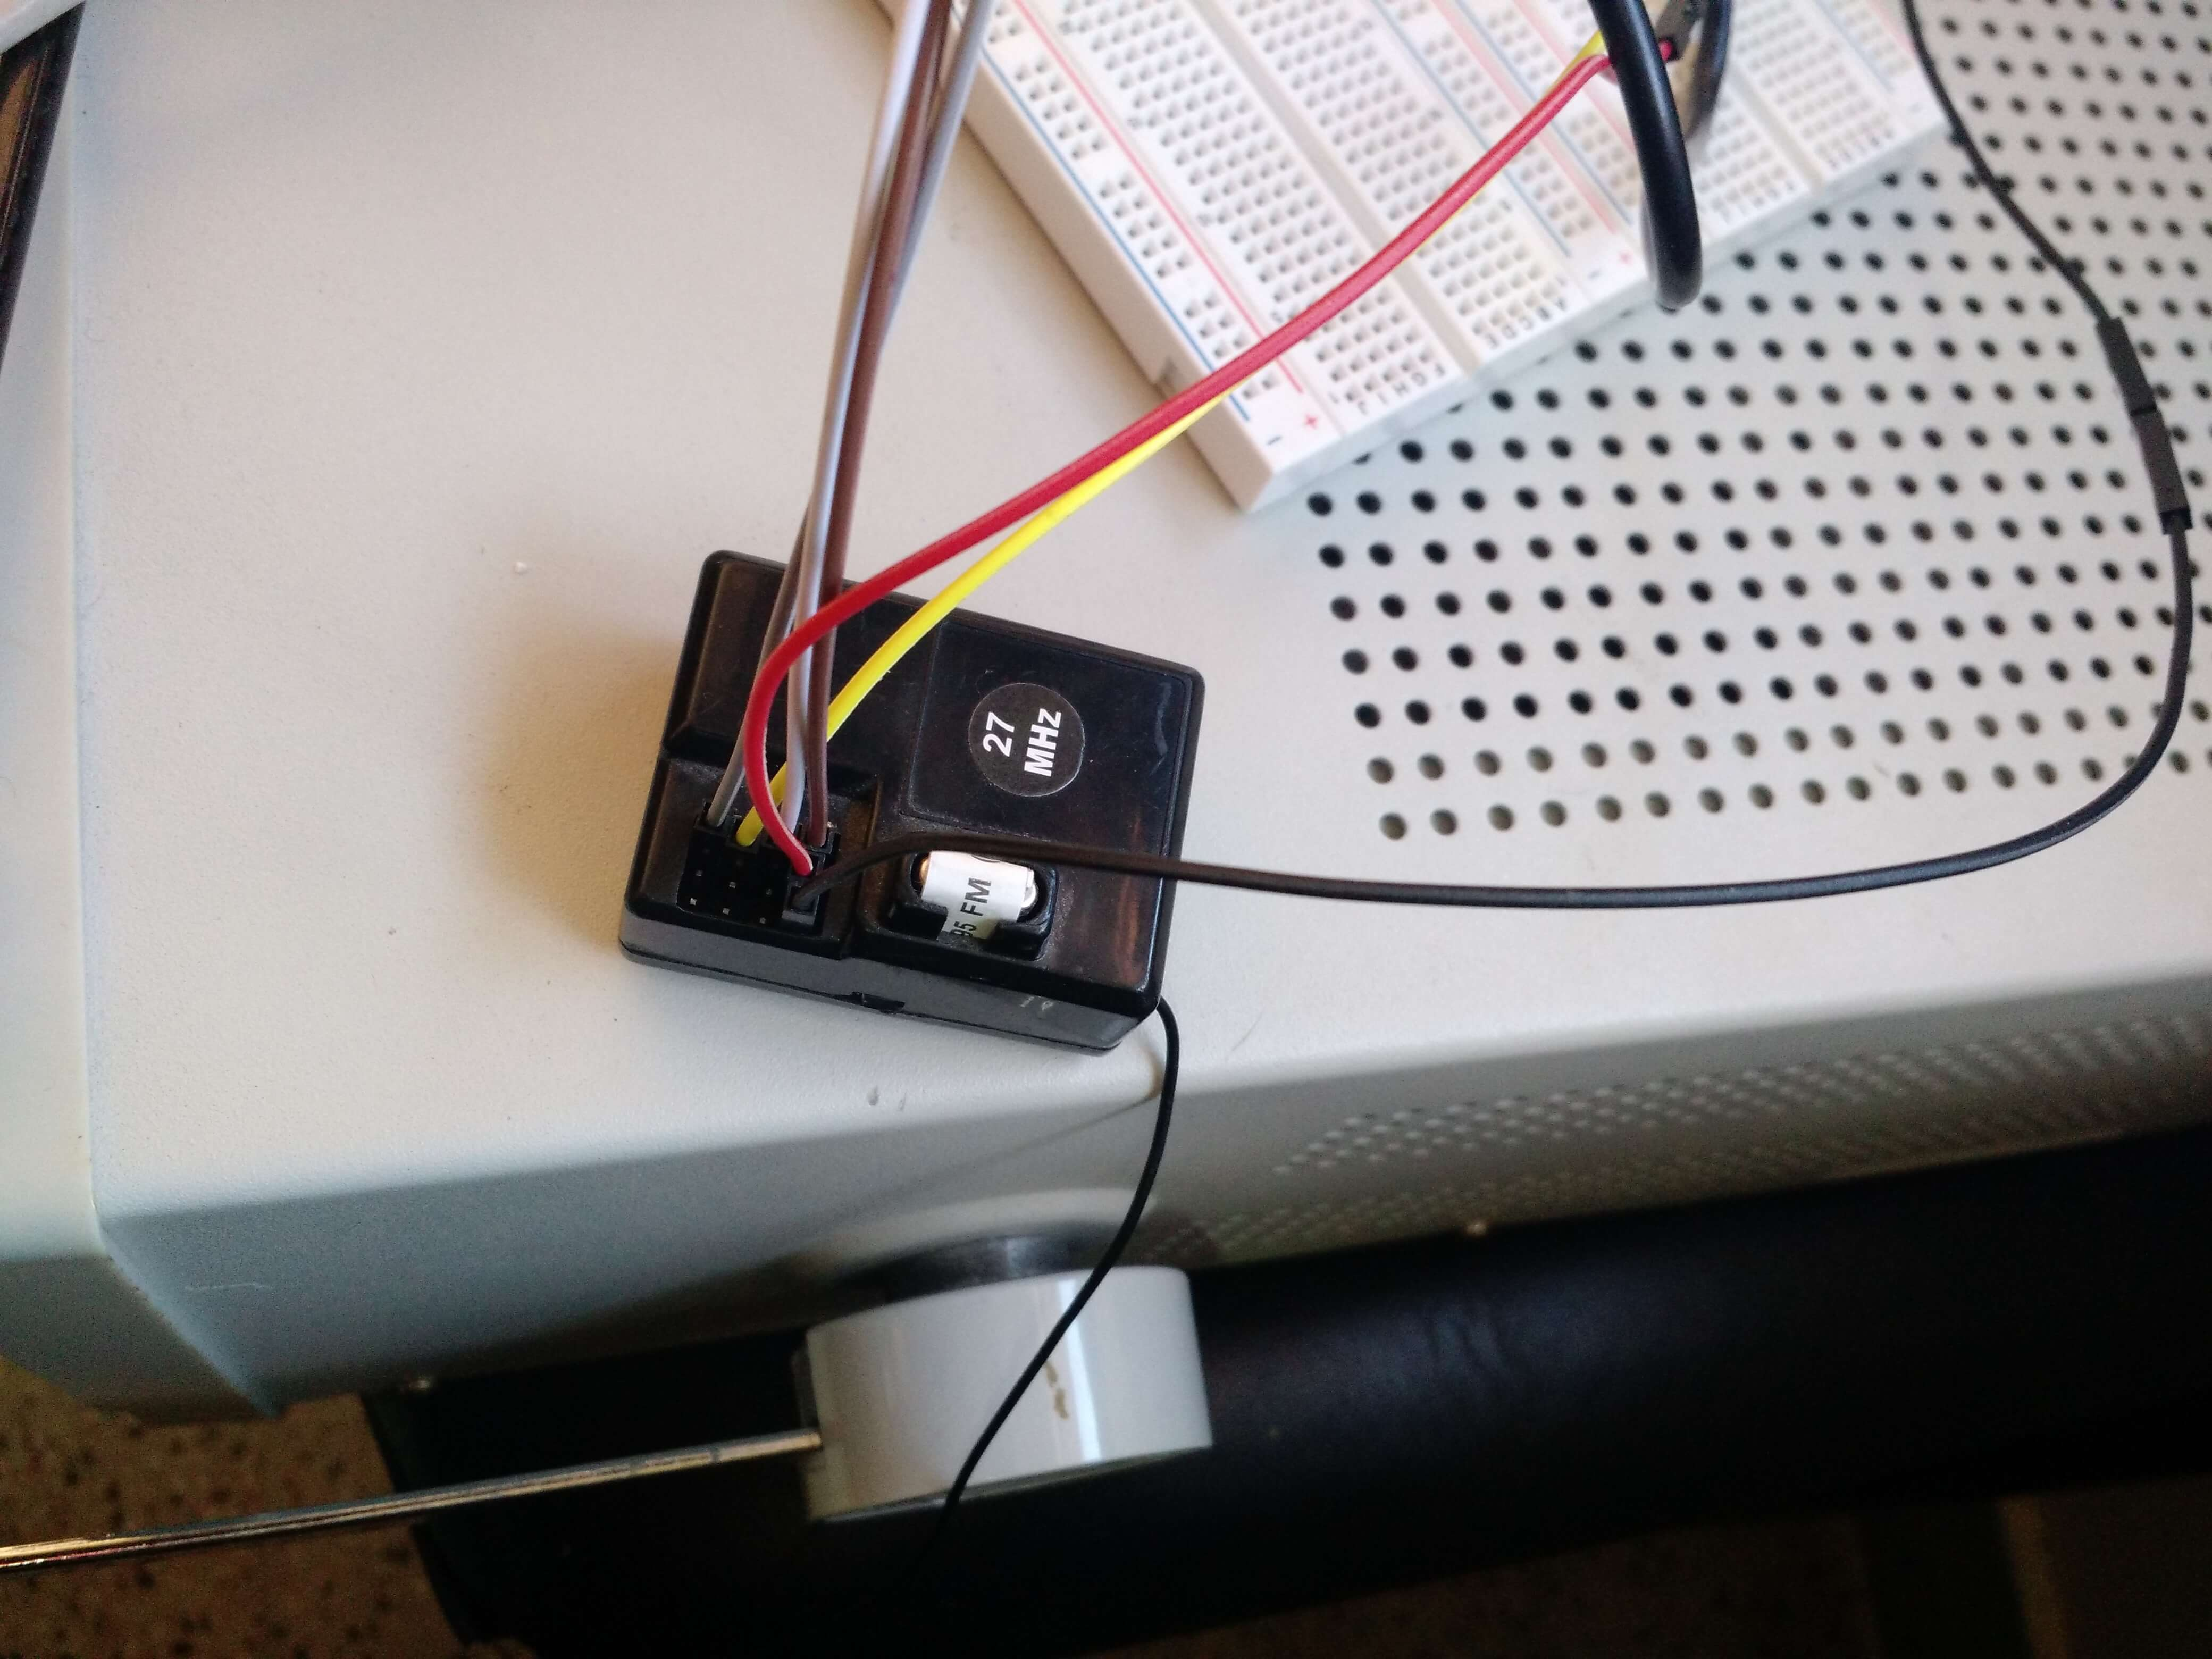
\includegraphics[width=0.5\linewidth, height=0.3\textheight]{Imagenes/fotos/rc_receptor}
		\caption{Receptor o Rx de 4 canales}
		\label{fig:rc_receptor}
		\end{figure}
		
		\begin{figure}[h!]
		\centering
		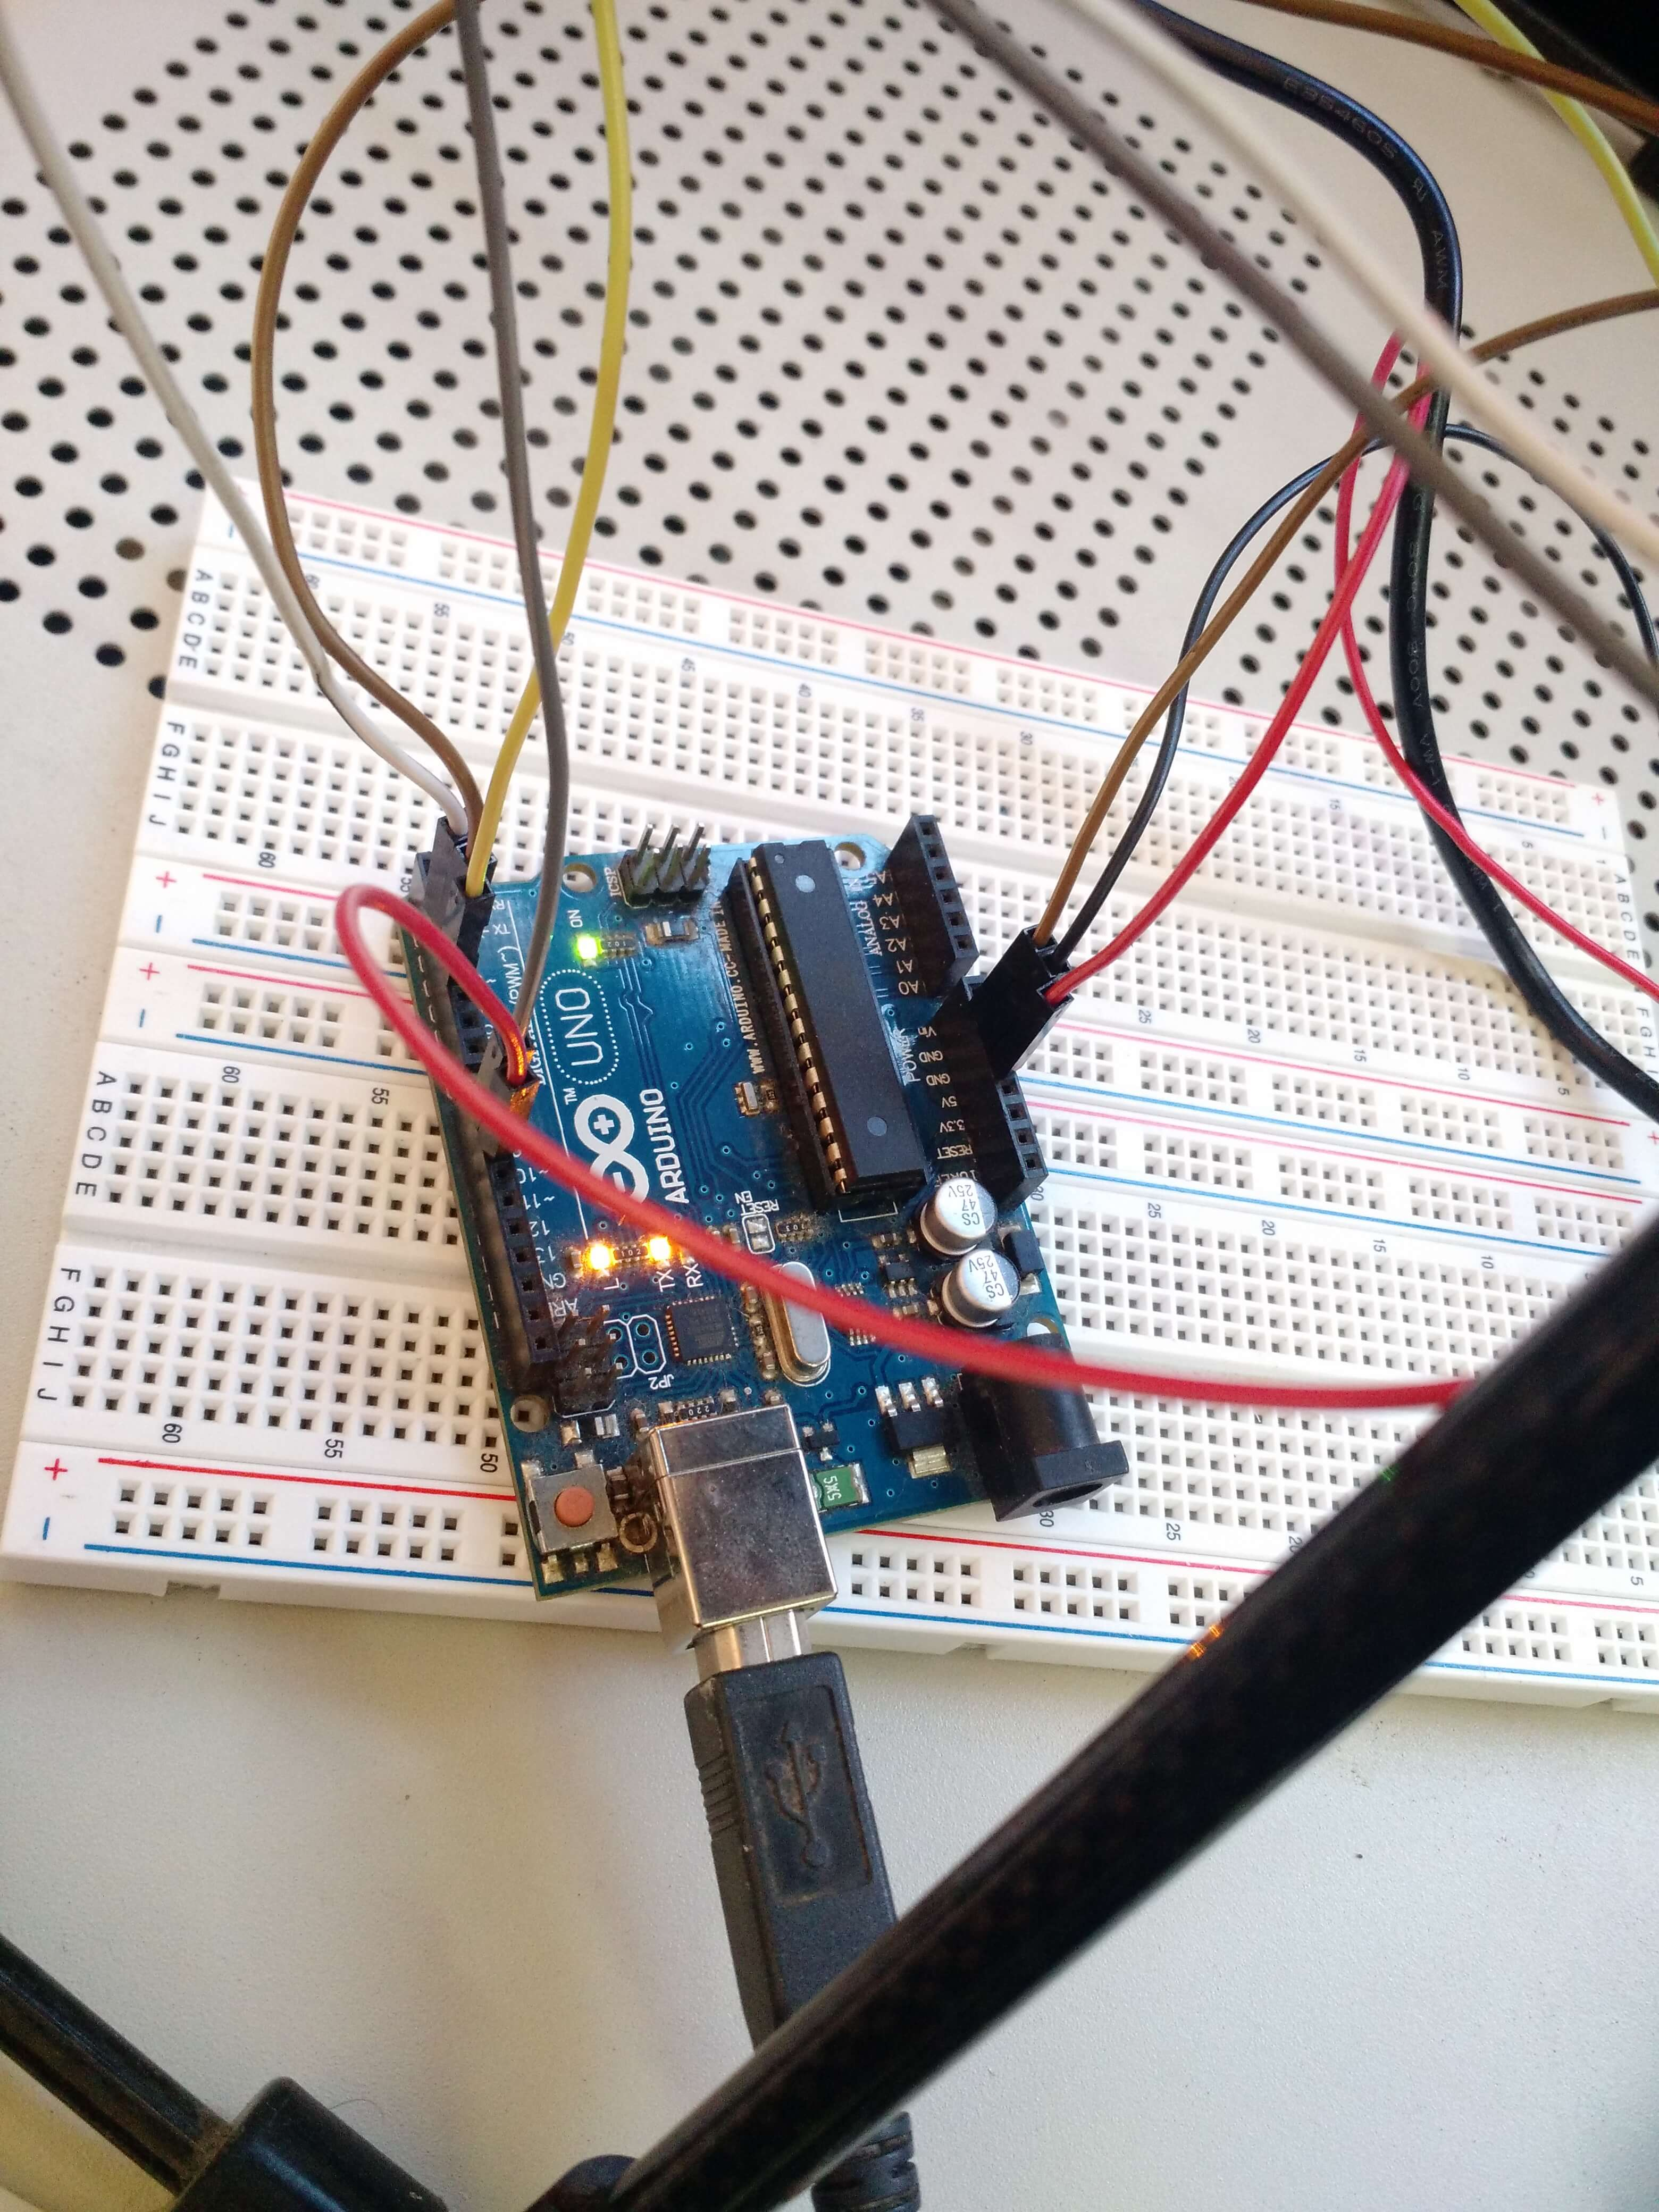
\includegraphics[width=0.5\linewidth, height=0.3\textheight]{Imagenes/fotos/arduino_ppm}
		\caption{Codificador PWM a SBUS implementado sobre Arduino.}
		\label{fig:arduino_ppm}
		\end{figure}
		
		
		\par Con respecto a las conexiones el�ctricas que lleva el cuadric�ptero, recurrimos en basarnos en la Figura \ref{fig:instnavio1}, donde muestra gr�ficamente el orden que llevan las conexiones con sus respectivos cables de colores. 
		
		\begin{figure}[h!]
		%TODO: Modificar imagen (esta mal el cableado de alimentacion de los motores)
		\centering
		\includegraphics[width=0.9\linewidth, height=0.4\textheight]{Imagenes/inst_navio1}
		\caption{Esquema de conexiones}
		\label{fig:instnavio1}
		\end{figure}
		
		Un aspecto a tener en cuenta es que no todos los componentes que se visualizan en la Figura \ref{fig:instnavio1} est�n presentes al momento de la instrumentaci�n ya que los dispositivos marcados con los n�meros (1,2 y 3) son de tipo comunicaci�n y se supone que con el m�dulo interno de \textit{Wifi} podr�amos sustituir estos elementos. 
		\par Por lo tanto se procede a realizar las conexiones mostradas. En primera medida se inicia conectando los motores del cuerpo del cuadric�ptero con los pines de la Navio2 como se puede observar en la imagen \ref{fig:conexionmotores}
		
		\begin{figure}[h!]
			\centering
			\includegraphics[width=0.4\linewidth, height=0.3\textheight]{Imagenes/fotos/conexion_motores}
			\caption{Conexi�n de datos a los motores.}
			\label{fig:conexionmotores}
		\end{figure}
		
		Despu�s de haber hecho las conexiones correspondientes a los motores, es necesario suministrarle energ�a de alg�n tipo de fuente para realizar las pruebas iniciales, es por eso que antes de conectar la bateria LiPo se considera la siguiente cuesti�n: ya que esta tiene una carga �til limitada se decide utilizar una fuente variable regulable disponible en el laboratorio de electr�nica del \textit{sinc(i)}  con el objetivo de realizar las pruebas necesarias sin estar dependiendo de la carga de la bater�a. Antes de realizar la conexi�n se ajusta el voltaje seg�n la bater�a Lipo existente (12V), dejando libre la cantidad de Amperes para que consuma lo que necesite. La fuente utilizada se puede observar en la Figura  \ref{fig:fuentevr}
		
		\begin{figure}[h!]
		\centering
		\includegraphics[width=0.4\linewidth, height=0.3\textheight]{Imagenes/fotos/fuentevr}
		\caption{Fuente variable regulable.}
		\label{fig:fuentevr}
		\end{figure}
		
		En la Figura \ref{fig:instnavio1} se puede ver que la bater�a suministra energ�a a los cuatro motores y al veh�culo, por lo tanto se decide alimentar al veh�culo con el transformador de f�brica y suministrar energ�a a  los motores con la fuente. Esta fuente como se puede observar en la Figura \ref{fig:fuentevr} contiene un �nico par de salida (positivo y negativo) por lo que es necesario multiplexar esta salida a 4 par de salidas m�s. Para eso se decide armar y soldar un conjunto de cables con sus respectivos conectores quedando de la siguiente manera.

%\begin{figure}[h!]
%\centering
%\includegraphics[width=0.5\linewidth, height=0.4\textheight]{Imagenes/fotos/IMG_20170601_131119448}
%\caption{Multiplexor}
%\label{fig:img20170601131119448}
%\end{figure}

Por �ltimo, se verifican las conexiones pertinentes a los planos y se buscan imperfectos en las uniones, en caso de encontrar alg�n tipo de estos se procede a repararlos. 
\begin{figure}[h!]
\centering
\includegraphics[width=0.5\linewidth, height=0.4\textheight]{Imagenes/fotos/quad_armado}
\caption{Cuadric�ptero armado para verificar funcionamiento.}
\label{fig:terminado}
\end{figure}


\subsection{Prueba de funcionamiento inicial}
Como etapa final y con el objetivo de verificar el correcto funcionamiento de nuestro veh�culo, se inicia el proceso de calibraci�n de sensores, para eso se decide utilizar \textbf{Mavproxy} seleccionando el m�dulo de calibraci�n y consecuentemente realizando los pasos que se nos indican de manera sencilla como se puede observar en la Figura \ref{fig:calibmavproxy}. 

Una vez concluida la etapa de calibraci�n se procede a enviar misiones de prueba, como por ejemplo elevarse del suelo 1 metro desde la posici�n inicial sin tener instalado las h�lices por motivos de seguridad, d�ndonos como resultados que el veh�culo interpreta los comandos. Aunque estas pruebas fueron realizadas de modo superficial en el capitulo \ref{cap4:pruebas} se profundizar� que el funcionamiento integral de los componentes responda de manera correcta.


\begin{figure}[h!]
\centering
\includegraphics[width=0.8\linewidth, height=0.4\textheight]{Imagenes/calibMavproxy}
\caption{Ejecuci�n del modulo de calibraci�n de MavProxy}
\label{fig:calibmavproxy}
\end{figure}


% Variable local para emacs, para  que encuentre el fichero maestro de
% compilaci�n y funcionen mejor algunas teclas r�pidas de AucTeX
%%%
%%% Local Variables:
%%% mode: latex
%%% TeX-master: "../ManualTeXiS.tex"
%%% End:
    % Desarrollo de la plataforma
% -*-coding: iso-latin-1  -*-
%---------------------------------------------------------------------
%
%                          Cap�tulo 3
%
%---------------------------------------------------------------------
%
% 03Edicion.tex
% Copyright 2009 Marco Antonio Gomez-Martin, Pedro Pablo Gomez-Martin
%
% This file belongs to the TeXiS manual, a LaTeX template for writting
% Thesis and other documents. The complete last TeXiS package can
% be obtained from http://gaia.fdi.ucm.es/projects/texis/
%
% Although the TeXiS template itself is distributed under the 
% conditions of the LaTeX Project Public License
% (http://www.latex-project.org/lppl.txt), the manual content
% uses the CC-BY-SA license that stays that you are free:
%
%    - to share & to copy, distribute and transmit the work
%    - to remix and to adapt the work
%
% under the following conditions:
%
%    - Attribution: you must attribute the work in the manner
%      specified by the author or licensor (but not in any way that
%      suggests that they endorse you or your use of the work).
%    - Share Alike: if you alter, transform, or build upon this
%      work, you may distribute the resulting work only under the
%      same, similar or a compatible license.
%
% The complete license is available in
% http://creativecommons.org/licenses/by-sa/3.0/legalcode
%
%---------------------------------------------------------------------

\chapter{Desarrollo de la plataforma}
\label{cap3:desarrollo}

\begin{FraseCelebre}
\begin{Frase}
Mi trabajo en el software libre est� motivado por un objetivo idealista: difundir libertad y cooperaci�n. Quiero motivar la expansi�n del software libre, reemplazando el software privativo que proh�be la cooperaci�n, y de este modo hacer nuestra sociedad mejor.
\end{Frase}
\begin{Fuente}
	-Richard Stallman-
\end{Fuente}
\end{FraseCelebre}

\begin{resumen}
	En este capitulo se describir� todo el proceso realizado de la fase denominada \textbf{Desarrollo de la plataforma}, que forma parte del presente proyecto . En esta fase se contempla las tareas del \textit{Dise�o detallado de la plataforma} y \textit{Codificaci�n} del mismo. En aspectos generales se define de manera un poco m�s especifica y en base al desarrollo global ya realizado en etapas anteriores, todo el comportamiento que incluir� la plataforma, como pueden ser, las funcionalidades de cada m�dulo, la interfaz gr�fica de usuario o por sus siglas en ingl�s (GUI), la l�gica interna correspondiente a cada uno y sus respectivas interacciones. 
\end{resumen}
\newpage
%-------------------------------------------------------------------
\section{Introducci�n}
%-------------------------------------------------------------------
\label{cap3:sec:Introduccion}

	\par En el �mbito inform�tico, como es sabido, la etapa de codificaci�n del software generalmente es la que m�s tiempo abarca con respecto a la duraci�n total del proyecto. Por esta raz�n, no es de sorprender que a medida que vayamos avanzando  objetivos, herramientas, planificaci�n, dise�o y l�gica del software est�n bajo un constante cambio ya que se van presentando obst�culos, alternativas e incompatiblididades que no han sido previstos en etapas iniciales. De esta manera, se ir�n ilustrando durante este capitulo capturas del estado del proyecto en distintas etapas del mismo, con el objetivo de poder ver el crecimiento y las t�cnicas utilizadas a medida que el proyecto va evolucionando y de esta manera poder aprender, para pr�ximos proyectos, las estructuras que uno debe implementar en etapas iniciales con el fin de no cometer los mismos errores.

\section{Dise�o detallado de la plataforma}
\label{cap3:sec:Disenio_detallado}

\begin{center}
	\begin{minipage}{0.9\linewidth}
		\vspace{5pt}%margen superior de minipage
		{\small
			\textit{Un dise�o de software es una descripci�n de la estructura del software que se va a implementar, los datos que son parte del sistema, las interfaces entre los componentes del sistema y, algunas veces, los algoritmos utilizados.}
		}
		\begin{flushleft}
			(Ian Sommerville, 2005, p71)
		\end{flushleft}
		\vspace{5pt}%margen inferior de la minipage
	\end{minipage}
\end{center}


Antes de iniciar directamente con la codificaci�n, ya que por el mismo instinto de cumplir con las restricciones de tiempo, uno necesita finalizarlo lo antes posible; pero antes que nada es necesario, realizar un dise�o de todo lo que queramos hacer, esto genera una linea de ejecuci�n a seguir que ayuda al ejecutor del proyecto tener planificado las tareas generales que debe realizar en el transcurso del proyecto y no estar pendiente de como proseguir una vez finalizada cada tarea y re-planificar constantemente el hilo del proyecto. Es por tal motivo que el presente proyecto se ha dividido la fase de dise�o en dos, la primera es un dise�o global, meramente con la intensi�n de contar con un panorama general del comportamiento del software/hardware y adem�s, poder mitigar la incertidumbre del ejecutor del proyecto, ya que se est� iniciando en el desarrollo de proyectos de esta envergadura. En base a la documentaci�n que se ha hecho en etapas anteriores podemos empezar a entablar de forma m�s precisa los procedimientos o tareas a realizar, lo que conlleva encarar la segunda parte del dise�o.


\par Seg�n Pressman esta etapa produce los siguientes dise�os:

\begin{itemize}
	\item \textbf{Dise�o de datos: } El dise�o de datos esencialmente se encarga de transformar el modelo de dominio de la informaci�n creado durante el an�lisis \cite{pressman88is}. 
	En el caso particular de este proyecto el dise�o de datos no juega un papel determinante dado que la herramienta de software propuesta, de la manera en que sea f�sicamente desarrollada e implementada, no requiere moment�neamente estructuras de datos complejas, ni de un esquema de bases de datos como ejemplo.	
	\item \textbf{Dise�o arquitect�nico: } En el dise�o arquitect�nico se definen las relaciones entre los principales elementos estructurales del programa \cite{pressman88is}. 
	Cuando se habla de elementos estructurales, se hace referencia entidades l�gicas que componen la arquitectura de nuestro dise�o, dentro del abanico de posibilidades de dise�os, podemos seleccionar, diagramas de flujo de datos, modelos de entidad-relaci�n, diagramas de clases, casos de usos entre otros esquemas gr�ficos. Viendo todas estas posibilidades, podemos encarar a dise�ar nuestra estructura con el modelo que m�s se ajuste a nuestras necesidades y sea lo m�s �til posible para las etapas posteriores. Por tal raz�n, es necesario de un dise�o que sea lo m�s representativo posible en el momento de codificaci�n, que utilice un paradigma orientado a objetos , ya que queremos representar objetos como veh�culos, posici�n geogr�fica, Joystick, etc; y que adem�s tengan cada uno sus correspondientes atributos, es por eso que seleccionamos un dise�o orientado a objetos, utilizando lo que anteriormente llamamos \textit{Diagramas de clases}. Estos diagramas son de suma utilidad ya que muestran de manera f�cil como ser� la estructura de nuestro c�digo y sus correspondientes relaciones entre cada uno, con el prop�sito de facilitar la tarea en las etapas posteriores al mismo.	
	\item \textbf{Dise�o de interfaz: } El dise�o de interfaz describe c�mo se comunica el software consigo mismo, con los sistemas que operan con �l, y con los operadores que lo emplean\cite{pressman88is}. 
	Dentro del aspecto de comunicaci�n de software consigo mismo y con otros sistemas es contemplado en el �tem anterior con el tipo de dise�o elegido. Aqu� lo que nos incumbe es la interacci�n con el operador del software. De esta manera, se selecciona una herramienta que nos permita realizar nuestra interfaz gr�fica del usuario, como por ejemplo, botones, \textit{label}, gr�ficos, \textit{checkboxes}, etc. ayudando al usuario a realizar sus respectivas tareas sin entrar en tanto detalle en comandos espec�ficos  que se debe memorizar con el fin de ser lo m�s amigable posible.
	\item \textbf{Dise�o procedimental: } El dise�o procedural transforma elementos estructurales de la arquitectura del programa en una descripci�n procedural de los componentes del software \cite{pressman88is}. 
	Para no ser extensos en lo que es el desarrollo de este proyecto y teniendo en mente que el tama�o del mismo no corresponde a uno de grandes dimensiones y  considerando que �nicamente  existe un �nico programador para la etapa de desarrollo, se descarta este tipo dise�o.

\end{itemize}


\par Dentro de lo que es el conjunto de dise�os obtenidos en esta etapa es importante saber en que orden realizar cada una. Ya que cada dise�o esta relacionado directamente con los dem�s, y el desarrollo de uno terminar� condicionando el siguiente. Es por esto, que se analiza la opci�n de comenzar primero con el dise�o de arquitectura. Suponiendo dicha elecci�n se desarrolla el siguiente flujo:

\par En el dise�o orientado a objetos o m�s espec�ficamente, en la confecci�n del diagrama de clases se detallan los objetos mediante bloques gr�ficos denominados clases. Estas clases contienen todos los atributos correspondientes al objeto, como por ejemplo, la clase veh�culo puede contener: cantidad de h�lices, altura de vuelo, velocidad, posici�n, etc. Y adem�s, seg�n este dise�o contiene todas las acciones que puede realizar a trav�s de funciones; si continuamos con el ejemplo de veh�culo a�reo pueden ser: volar, aterrizar, despegar, etc. Esto nos brinda como resultado final una estructura al momento de implementar el c�digo, por lo que facilita la tarea del programador. Adem�s, y un punto importante a tener en cuenta es que muestra como se comunicar� cada clase con las dem�s, esta caracter�stica ayuda a descubrir que funciones extras son necesarias implementar para una correcta cooperaci�n en conjunto. Sin embargo, existe una desventaja, dentro del punto de vista de la interacci�n del usuario, es que no toma en cuenta las funcionalidades que puede desear el usuario para que el uso del software sea m�s placentero (que es el objetivo de este dise�o), sino que el resultado del dise�o se centra en que cada clase pueda responder a las necesidades (mensajes) de las dem�s clases. 


En cambio, si primero realizamos el dise�o de la interfaz gr�fica del usuario, nos determinar� que es necesario entre otros aspectos que no han sido incluido en el dise�o arquitect�nico ya que no se ha tomado como parte importante en el desarrollo, la interacci�n del usuario. Como por ejemplo, funciones de validaci�n de datos, ventanas de advertencias, gr�ficos, como es el HUD (figura \ref{fig:hud}).


\begin{figure}[h]
	\centering
	\includegraphics[width=0.5\linewidth, height=0.2\textheight]{Imagenes/hud}
	\caption{Head Up Display}
	\label{fig:hud}
\end{figure}

\par Como podemos ver y seg�n las restricciones presentes, es conveniente realizar primero un dise�o de interfaz, ya que el mismo nos proporcionar� m�s detalles de implementaci�n. Por tal motivo iniciamos primero con el dise�o de interfaz.

\subsection{Dise�o de interfaz}

En primera instancia se inicia con la interfaz gr�fica del usuario o su equivalente en ingles \textit{\textbf{G}raphical \textbf{U}ser \textbf{I}nterface}; por definici�n es el proceso que define como ser� la interacci�n entre el software y el usuario final. Para esto, se utiliza la herramienta Qt Designer, que proporciona mediante un panel de \textbf{widgets} todos los elementos necesarios para el dise�o del mismo. 

\par Para iniciar este proceso, nos basamos en los \textit{mockups}  desarrollados  en la fase de dise�o global de la plataforma, bas�ndonos pantalla por pantalla en la confecci�n de cada uno. Cabe mencionar que las pantallas presentes del dise�o han sido obtenidas luego de un arduo proceso de modificaciones y actualizaciones debido a las necesidades e inconvenientes que se iban presentando en el transcurso de la fase de codificaci�n. Las im�genes de la GUI se pueden ver en el anexo \ref{ap1:GUI}

\subsubsection{Modificaciones generales}
\begin{itemize}
	
	\item \textbf{Inserci�n del HUD en lugar de un mapa} Se ha considerado dise�ar el HUD, en lugar de un mapa. Ya que el mismo no se considera de suma importancia para la navegaci�n en un marco de referencia relativo. La implementaci�n del mapa, se ha documentado como un requisito para las versiones futuras de la plataforma.
	
	\item \textbf{Reemplazo de ubicaci�n de iconos de estados} Los iconos posicionados en la barra superior del software se han reubicados dentro de lo que es el HUD, ya que estos iconos sobrecargaban la aplicaci�n con una constante actualizaci�n siendo que el HUD es el encargado de mostrar dicha informaci�n de manera actualizada.
	
	\item \textbf{Sustracci�n de pesta�a \textit{Sensores}} Seg�n el requisito \textbf{Implementaci�n de calibraci�n de sensores} no se considera para esta versi�n la posibilidad de calibrar los sensores del veh�culo. Si, se incluyen los par�metros del veh�culo y sus respectivos valores en la pesta�a de configuraci�n, con el fin de ser configurados.
	
\end{itemize}



\subsection{Dise�o arquitect�nico}


Luego de finalizar con el dise�o de interfaz y en base al diagrama de clases realizado en etapas anteriores del proyecto, se inicia el modelado m�s detallado del diagrama de clases de nuestro proyecto. Para esto se utiliza de la herramienta ArgoUML \footnote{P�gina web de ArgoUML  http://argouml.tigris.org/ }, obteniendo como resultado el diagrama de clases adjuntado en el ap�ndice \ref{ap1:classDiagra_vFinal}

Para el desarrollo del mismo se ha considerado el dise�o de la interfaz gr�fica y de manera complementar�a ,la comunicaci�n que tiene con las dem�s clases conectadas, esto nos facilita al momento de determinar que tipo de funciones necesita cada una y la forma en que se los debe enviar dicha informaci�n.  



\section{Codificaci�n y Testing}

	En esta etapa consiste en traducir el dise�o en una forma legible por la m�quina. Por tanto, iniciaremos esta tarea seg�n los dise�os de diagrama de clases generados y siempre teniendo en mente los requerimientos estipulados por los \textit{stakeholders}.
	
	\par Seg�n, el diagrama de clases adjuntado en el ap�ndice \ref{ap1:classDiagra_vFinal} tenemos varias clases que se encargar�n de un grupo de funcionalidades en espec�fico y a su vez cada una brinda funcionalidades a sus clases vecinas, para entender un poco el funcionamiento del software comenzaremos explicando cada una, exceptuando las clases que se han utilizado de las librer�as pertinentes.
	
	%ANEXAR CODIGO?

		\subsection{Clase Veh�culo}

			\begin{figure}[h!]
				\centering
				\includegraphics[width=0.4\linewidth, height=0.35\textheight]{Imagenes/classVehiculo}
				\caption{Clase Veh�culo}
				\label{fig:classvehiculo}
			\end{figure}
		
			La clase Veh�culo es la responsable de representar en su mayor medida el objeto real, en nuestro caso es el cuadric�ptero.  Para esto se ha decidido asignarle las siguientes funcionalidades 
			
		\begin{itemize}
			
			\item \textbf{Funciones de vuelo: } Seg�n las restricciones establecidas en el ERS que se han estipulado en primera medida, ya sea por falta de conocimiento de librer�as y/o complejidad de los mismos, �nicamente las siguientes funcionalidades de vuelo \textbf{Ascenso, Descenso y Hovering}; en cambio, gracias a las librer�as utilizadas se han codificado m�s funcionalidades correspondientes a las maniobras que puede realizar el veh�culo. Dentro de este conjunto se desarrollaron las siguientes funciones (utilizando el protocolo MAVLink \textit{Micro Air Vehicle Link} y la librer�a Dronekit):
			
			
			\par Cabe mencionar que estas funcionalidades han sido dise�adas con la posibilidad de realizar acciones de vuelo en un marco de referencia global, utilizando las coordenadas globales proporcionadas por el GPS en base a la latitud, longitud y altura (figura \ref{fig:latlong}). Adem�s, es posible establecer sobre un marco de referencia relativo, es decir, este marco de referencia toma como origen el punto inicial de partida del veh�culo, por lo que las coordenadas que ingresemos tendr�n como referencia el punto de despegue. Es importante recordar que el marco de referencia global, conlleva la implementaci�n de un mapa y seg�n el requerimiento R025 este es opcional, e insistiendo con lo mencionado, esta funcionalidad se implementar� en futuras versiones.
			
			\begin{figure}[h!]
				\centering
				\includegraphics[width=0.7\linewidth, height=0.2\textheight]{Imagenes/latlong}
				\caption{Marco de referencia global.}
				\label{fig:latlong}
			\end{figure}
		
		
		
		
		\begin{enumerate}
			\item \textbf{Despegar:  } Esta funcionalidad env�a un comando al veh�culo especific�ndole que debe propulsarse gracias a sus motores a una altura en particular.  
			\item \textbf{Aterrizar: } Esta funci�n ordena al veh�culo que aterrice en un punto establecido, dependiendo del sistema de referencia, ya sea global o relativo.
			\item \textbf{Suspenderse: } Seg�n un punto en particular el veh�culo estar� inm�vil y suspendido en el aire por la cantidad de tiempo que se le asigne. Adem�s, esta funci�n entra en el requerimiento R017, donde se establece una funci�n de salvataje encargada de ejecutarse en caso de alg�n inconveniente o percance con el veh�culo y/o conexi�n. 
			\item \textbf{Ir a un punto en especifico: } Como bien su nombre lo especifica, esta orden y seg�n un sistema de referencia le indica al veh�culo que debe desplazarse en un punto en particular. 
			\item \textbf{Volver a inicio: } El veh�culo almacena en primeras instancias su posici�n inicial, asign�ndola en una variable interna llamada \textit{home}, una vez que esta orden ha sido enviada, el veh�culo tratar� de dirigirse a su punto de partida.
			\item \textbf{Moverse: } Seg�n el requerimiento R024, que establece distintos tipos de vuelo se han codificado las funciones de \textit{velocidad} y \textit{yaw} que seg�n las ordenes enviadas de un Joystick el veh�culo modificar� su direcci�n en tiempo real,  ya que se han restringido estos comandos a que tengan una duraci�n de ejecuci�n m�nima, dando as� lugar a un nuevo comando y captar las nuevas indicaciones que han sido enviadas por el usuario.
			
		\end{enumerate}
		
		\item \textbf{Modo de vuelo: }
		Dentro del conjunto de las funcionalidades de vuelo se pueden observar que existen funciones con el prefijo "mis", estos a diferencia de los dem�s, son utilizados cuando el veh�culo se encuentro en modo AUTO, es decir, estos comandos ser�n enviados al veh�culo con el fin de que sean almacenados y ejecutados de manera secuencial misi�n por misi�n cuando se envi� la orden \textit{ejecutar misiones}. Para cumplir de manera complementar�a con el requisito R024, se han codificado funciones que gestionen las misiones pertinentes. 
		
		\item \textbf{Conexi�n: } En base a los requerimientos R015,R016 se han incluido en la clase veh�culo las funciones de \textit{conectado, desconectar y el constructor de la clase} estas son encargadas de conectarse de manera inal�mbrica a una red LAN, gracias a su m�dulo WiFi instalado en la placa Raspberry Pi o de manera ad-hoc mediante m�dulos de comunicaci�n inal�mbrica conectados en un puerto serial. 
		
	\end{itemize}
	
	
	Por �ltimo una funci�n que asigna \textit{Callbacks} a los atributos del veh�culo, ya que estar consultando constantemente los cambios que se est�n produciendo dentro del veh�culo conlleva un consumo extra de recursos,por lo que se decide implementar una funci�n "setCallback2Param" que cada vez que el atributo correspondiente sufra alg�n tipo de cambio, este llame a otra funci�n para informarle de dicha transici�n.
	\newpage
	
	\subsection{Clase Joystick}

	
		La clase Joystick, es la encargada de gestionar dentro del los comandos conectados en el equipo, sus respectivas acciones que han sido ejecutadas por el usuario. 
		
		\begin{figure}[h!]
			\centering
			\includegraphics[width=0.4\linewidth, height=0.3\textheight]{Imagenes/classJoystick}
			\caption{Clase Joystick}
			\label{fig:classjoystick}
		\end{figure}
	
		\par Con la ayuda de la librer�a Pygame podemos obtener informaci�n de los joystick conectados como nombre, cantidad de botones, n�mero de ejes, si se ha presionado o saltado un bot�n, entre otras acciones, con el objetivo de poder interpretar, seg�n un mapeo de funciones que se han pre-configurado las acciones que desee realizar el usuario en modo manual sobre el veh�culo. Cabe mencionar que dicha clase se ha codificado satisfaciendo los requerimiento R012 y R022.
		
		



	\subsection{Clase Gr�fico Datos}
	
	
			
		\begin{figure}[h!]
			\centering
			\includegraphics[width=0.4\linewidth, height=0.3\textheight]{Imagenes/classGraficoDatos}
			\caption{Clase gr�ficos de datos o de atributos del veh�culo.}
			\label{fig:classgraficodatos}
		\end{figure}

		La clase Gr�fico de Datos fue creada con el fin de cumplir con el requerimiento R002 que solicita una representaci�n gr�fica en tiempo real y evolutiva de la informaci�n capturada. Para realizar dicha tarea en primer momento se ha utilizado la librer�a Vispy como la definici�n del requerimiento lo especifica; pero a medida que se iba avanzando en el desarrollo y prueba del mismo se ha encontrado el inconveniente de que dicha librer�a no contiene la documentaci�n actualizada, lo que genera contratiempos al momento de cumplir con el objetivo, por lo que se decide utilizar una librer�a con una comunidad m�s activa, como lo es PyQtGraph. Esta librer�a cuenta con una gran comunidad activa y una documentaci�n detallada de cada funcionalidad disponible, esto facilita mucho al ejecutor del proyecto a dirigir la atenci�n en otros aspectos del proyecto. Cabe destacar que esta librer�a, m�s all� de contener las funcionalidades necesarias para cumplir con el requerimiento estipulado.
	
		\begin{figure}[h!]
			\centering
			\includegraphics[width=0.7\linewidth, height=0.3\textheight]{Imagenes/GD_prueba}
			\caption{Prueba animada en la inserci�n de dato utilizando la Clase Gr�fico Datos.}
			\label{fig:gdprueba}
		\end{figure}
	
		Entre el conjunto de funcionalidades disponibles, se describen las m�s importantes:
	
		\begin{itemize}
			\item \textbf{Cupo m�ximo de lineas: } Con fines est�ticos se ha implementado la opci�n de disponer de un n�mero m�ximo de gr�ficos en pantalla, ya que el acumulamiento de gr�ficos sobrecargar� a la aplicaci�n de recursos a consumir y adem�s dejar� de apreciarse cada gr�fica en la ilustraci�n por motivos de espacio. En caso de asignar una nueva linea al gr�fico correspondiente, el mismo eliminar� el primer gr�fico ingresada, utilizando una metodolog�a tipo FIFO.
			\item \textbf{Identificaci�n de lineas: } Para poder gestionar las lineas presentes en el gr�fico es necesario asignarle a cada una un identificador, este identificador adem�s servir� para las clases antecesoras para la inserci�n y eliminaci�n de cada una.
			\item \textbf{Pausado de animaci�n: } Es de esperar que el gr�fico no este disponible tiempo completo, por lo que se decide incorporar la opci�n de pausado de la animaci�n con el prop�sito de optimizar el uso de recursos del equipo y que la aplicaci�n BEcopter sea lo m�s liviana posible.
			
		\end{itemize}


	\subsection{Clase HUD} %R003
	
		La clase HUD o por su respectiva traducci�n, \textit{visualizaci�n cabeza-arriba}, es la encargada de visualizar al piloto, en este caso el usuario, los datos m�s relevantes del estado del veh�culo, con el objetivo de tener a simple vista el comportamiento del mismo en tiempo real. Por su parte, en el �mbito aeron�utico se utilizan ciertos instrumentos de navegaci�n o s�mbolos que informan al piloto el estado de la aeronave, ya sea, velocidad, altitud, inclinaci�n, etc; que para el desarrollo de esta clase es conveniente saber su significado. Por tal raz�n, explicaremos cada uno de estos instrumentos con su respectiva representaci�n gr�fica.
		
		
		\begin{figure}[h!]
			\centering
			\includegraphics[width=0.4\linewidth, height=0.5\textheight]{Imagenes/classHUD}
			\caption{Clase Head Up Display}
			\label{fig:classhud}
		\end{figure}

\newpage

		\subsubsection{Instrumentos de navegaci�n }
			Son los instrumentos esenciales para poder orientarse y seguir la ruta deseada por parte del piloto. \\	
			
			\textbf{Horizonte artificial}
			
				\begin{wrapfigure}{l}{0.3\linewidth}
					\centering
					\includegraphics[width=0.8\linewidth]{Imagenes/horizonte_artificial}
					\caption{Horizonte artificial indicando un giro a la derecha en descenso.}
					\label{fig:horizonte_artificial}
				\end{wrapfigure}
	
				
				El horizonte artificial muestra la orientaci�n longitudinal de la aeronave (la relaci�n del eje longitudinal del avi�n con respecto al plano del suelo), es decir: si est� girado, inclinado, con la frente del veh�culo levantado, bajado o todo a la vez. Sirve de gran ayuda en condiciones en que la visibilidad es poca o nula. El horizonte artificial tiene dos partes: el horizonte propiamente dicho, y el indicador de rumbo. El primero est� compuesto por una regi�n azul que representa el cielo, otra normalmente marr�n que representa la superficie terrestre, una mira que representa la direcci�n en que apunta la frente de la aeronave, y varias marcas a su alrededor. Las marcas horizontales a ambos lados representan las alas, el plano de la aeronave, y su �ngulo con el l�mite entre las regiones de cielo y superficie (el horizonte artificial), el cual con dichos planos se produce el �ngulo de alabeo. Dispuestas verticalmente a intervalos regulares, hay marcas horizontales m�s peque�as que representan �ngulos concretos en el plano vertical, a intervalos de 5�, 10�, etc. Muestran el �ngulo actual del eje longitudinal con el plano del suelo. Su principio mec�nico es basado sobre un giroscopio.

%
			\textbf{Indicador de rumbos }
			
				\par El indicador de rumbo, o giroscopio direccional, proporciona al piloto la direcci�n de la aeronave en grados magn�ticos. 
				
				\begin{figure}[h!]
					\centering
					\includegraphics[width=0.2\linewidth, height=0.2\linewidth]{Imagenes/indicador_rumbo}
					\caption{Indicador de rumbos}
					\label{fig:indicadorrumbo}
				\end{figure}
	%
			
			\textbf{Coordinador de Giro}
			
				\par En el coordinador de giro vemos en lugar del bast�n una Figura de un avi�n que nos indica el grado de inclinaci�n de las alas.
				
				
				\begin{figure}[h!]
					\centering
					\includegraphics[width=0.3\linewidth, height=0.3\linewidth]{Imagenes/coord_de_giro}
					\caption{Coordinador de giro.}
					\label{fig:coord_de_giro}
				\end{figure}

				\par Una vez concientizado en los instrumentos de vuelo se procede a integrarlos de manera simulada en un \textit{widget}, con el fin de que cumpla las mismas funcionalidades. Para empezar necesitaremos de una librer�a gr�fica en el cual nos proporcione de funcionalidades para poder graficar estos instrumentos, para eso se selecciona la conocida librer�a OpenGL. Dicha librer�a est� equipada de funcionalidades para dibujar escenas tridimensionales complejas a partir de primitivas geom�tricas simples, tales como puntos, l�neas y tri�ngulos. Adem�s nos d� a disposici�n la personalizaci�n de todos los paramentos que est�n dentro de una escena como posici�n de la luz, c�mara,  tipo de materiales y luces. Pero m�s all� de todo este conjunto de herramientas que nos deja a disposici�n OpenGL, la tarea del dise�o del HUD es realizar en un dibujo en 2D,  el cual se mostraran un conjunto de datos y lineas b�sicas, por lo que se decide no utilizar directamente esta librer�a para el dise�o de la escena, sino que se busca de una \textit{API} en que podamos graficar nuestros instrumentos de navegaci�n de forma m�s sencilla, es por eso, que sea realiza una investigaci�n antes de utilizar dicha librer�a y se encuentra que la librer�a PyQt, en sus conjuntos de clases contiene una de nombre QPainter, m�s all� que internamente usa OpenGL, esta librer�a facilita un conjunto de funciones tales como dibujar elipse, texto, im�genes, lineas, entre otras funcionalidades y de una manera m�s comprensible. De esta forma, abordamos la tarea de graficar  la escena de la siguiente manera: \newline

				\begin{enumerate}
					
					\item \textbf{Dibujo del Horizonte Artificial}
						El horizonte artificial como se puede observar en la Figura \ref{fig:horizonte_artificial} est� compuesto por dos rect�ngulos, uno representando el cielo y el segundo la tierra, de esta manera, con la funcionalidad de QPainter que nos proporciona dibujar un rect�ngulo proseguimos a dibujar dos rect�ngulos simulando el horizonte artificial; qued�ndonos como se puede ver en la Figura \ref{fig:hudv0}.
						\begin{figure}[h!]
							\centering
							\includegraphics[width=0.3\linewidth, height=0.3\linewidth]{Imagenes/HUD_v0}
							\caption{HUD v0.1}
							\label{fig:hudv0}
						\end{figure}
						
						\par Hasta aqu�, podemos observar que la Figura \ref{fig:hudv0} satisface las necesidades de representar el horizonte artificial seg�n nuestras especificaciones, pero al momento de proyectar al uso del mismo podemos encontrar los siguientes problemas:
						
						\begin{enumerate}
						
					\item \textbf{Problema gr�fico al momento del Roll: } Como se puede ver en la Figura \ref{fig:hudv0e1} , cuando la escena sufre una rotaci�n sobre su eje perpendicular, es decir, simulando un giro sobre el Roll o alabeo del veh�culo, la imagen muestra imperfecciones en las puntas del recuadro. 
						
						\begin{figure}[h]
							\centering
							\includegraphics[width=0.3\linewidth, height=0.3\linewidth]{Imagenes/HUD_v0_e1}
							\caption{Error gr�fico al momento de rotar}
							\label{fig:hudv0e1}
						\end{figure}
						
						\subitem Este problema f�cilmente se puede solucionar ampliando los tama�os de los rect�ngulos en ambas direcciones, considerando siempre el tama�o m�s largo entre el alto y ancho de la pantalla, ya que si no tenemos en cuenta este aspecto cuando tengamos una imagen sumamente apaisada y de poca altura, obtendr�amos el mismo problema. Por tal motivo, se debe elegir un tama�o adecuado para la imagen; ahora la pregunta es �Qu� tama�o debo asignarle a la imagen para que no se presenten dichos defectos? 
			
		
							\textbf{Obtenci�n de la longitud requerida}
		
							\begin{figure}[h]
								\centering
								\includegraphics[width=0.3\linewidth, width=0.3\linewidth]{Imagenes/problemaPuntas}
								\caption{Problema gr�fico en las esquinas}
								\label{fig:problemapuntas}
							\end{figure}
							Como bien muestra la Figura \ref{fig:problemapuntas}, cuando la imagen de fondo sufre una rotaci�n no llega a cubrir lo suficiente los limites de la pantalla, por tanto, se  produce dicho problema. De tal manera se debe buscar la longitud m�xima que debe tener la imagen para que cubra dichos limites, en la Figura  \ref{fig:problemapuntas} se puede apreciar una linea roja que representa el largo necesario a calcular. Este deber� ser la m�nima longitud que deben tener el alto y ancho de la imagen, es decir :
							
							\begin{center}
								$L > Ancho_{Imagen}  \land L > Alto_{Imagen}   $ 
							\end{center}
						
							Para calcular dicho valor, se propone implementar una circunferencia con centro en el origen de la pantalla y que tenga un radio por el cual cubra por completo los limites del mismo, como se puede observar en la Figura \ref{fig:problemapuntas2}, de esta manera se contemplan las posibilidades de que la imagen de fondo cubra por completo el dominio de la pantalla en cualquier angulo de rotaci�n que sufra. 
							\begin{figure}[h]
								\centering
								\includegraphics[width=0.3\linewidth, width=0.3\linewidth]{Imagenes/problemaPuntas2}
								\caption{Circunferencia con radio que satisface la longitud requerida.}
								\label{fig:problemapuntas2}
							\end{figure}
							
							\par Por �ltimo, obtener esta longitud se traduce en un problema trigonom�trico  donde se debe obtener la hipotenusa de un triangulo rect�ngulo con base $w/2$ y alto $h/2$. Utilizando el teorema de pit�goras obtenernos que
							
							
							\begin{subequations}\label{eq:longRequerida}
								\begin{align}
								R &= \sqrt{(\frac{w}{2})^2 + (\frac{h}{2})^2}  \\
								R &= \frac{1}{2} (w + h) \label{eq:longRequerida1}
								\end{align}
							\end{subequations}
							
							Como podemos apreciar, la longitud m�nima requerida se obtiene de la ecuaci�n \ref{eq:longRequerida1}. Pero como es de saber, este valor es la longitud total m�nima que debe tener tanto el alto como el ancho de la imagen, por lo que se debe conocer cual es la diferencia al que debemos agregar al ancho, como tambi�n al alto de la imagen. Para esto, simplemente realizamos la diferencia para cada atributo y obtendremos el siguiente valor a agregar
							
							
							\begin{subequations}
								\begin{align}
								Ancho_{aux} &= \frac{1}{2} (h+w) - \frac{w}{2} =  \frac{h}{2} \\
								Alto_{aux} &=  \frac{1}{2} (h+w)  - \frac{h}{2} =  \frac{w}{2} 
								\end{align}
								
							\end{subequations}
					
					\item \textbf{Problema al simular el Pitch: } Otro problema que surge, es al momento de simular el cabeceo o pitch, es que dentro de la escena cuando ocurre este comportamiento el script debe realizar un transformaci�n de traslado, siendo proporcional a la inclinaci�n ocurrida en el veh�culo. Pero en cambio, el defecto que ocasiona es que �nicamente se trasladar�n los dos cuadrados ya dibujados, dejando al descubierto el \textit{background}, como se puede ver en la Figura \ref{fig:hudv0e2}. Adem�s, hay que tener en cuenta que la escena debe permitir un pitch de 0 a 360 grados, por lo que se tendr� que expandir la escena con el fin de simular un entorno virtual 360 en 3D.
								
						\begin{figure}[h!]
							\centering
							\includegraphics[width=0.3\linewidth, height=0.3\linewidth]{Imagenes/HUD_v0_e2}
							\caption{Error al momento de simular el Pitch}
							\label{fig:hudv0e2}
						\end{figure}
			
		Para solucionar este inconveniente surgen las siguientes propuestas 
		
		\begin{enumerate}
			\item \textbf{Mapear una textura al rededor de la c�mara, mediante coordenadas esf�ricas: } En esta propuesta se debe generar una textura de ambiente exterior por el cual ser� mapeada de tal manera que simular� un ambiente 3D. La desventaja de esta propuesta es que la clase QPainter no proporciona funcionalidades para el desarrollo de dibujos en 3D, ni tampoco sus clases antecesoras para el mapeo de textura. Por lo cual, se deber�a codificar la textura manualmente y utilizando las funcionalidades primitivas de OpenGL.
			
			\item \textbf{Inserci�n de rect�ngulos dependientes del Pitch: } Aqu� lo que se pretende es que a medida que el pitch aumente o disminuya, es decir, que el veh�culo cabecee para arriba o abajo, el script interprete estos datos para dibujar un nuevo rect�ngulo contrario al que se ve en pantalla (cielo/tierra), simulando un entorno infinito, como se puede ver en la Figura \ref{fig:addrectangle}.
			
			\begin{figure}[h]
				\centering
				\includegraphics[width=0.4\linewidth, height=0.2\textheight]{Imagenes/addRectangle}
				\caption{Insertando un rect�ngulo perteneciente al piso. }
				\label{fig:addrectangle}
			\end{figure}
			
			Siendo parecer la propuesta m�s efectiva, al momento de realizar las pruebas con el veh�culo se descubre que presenta inconsistencias, ya que el movimiento del pitch no es continuo, por tanto, no se puede ir llevando un seguimiento del cuadro que se esta viendo actualmente para la inserci�n del siguiente. M�s all� de poder emparchar esta propuesta anexando al algoritmo estructuras extras para el seguimiento de los cuadros, el prop�sito del mismo no es acomplejar el problema presente, de esta manera, se recurre al desarrollo de la siguiente propuesta.
			
			\item \textbf{Mapeo del Pitch sobre una imagen: } Finalmente, para solucionar el presente problema, y siempre reduciendo la complejidad a una soluci�n, se propone dibujar una imagen que contenga la escena del horizonte artificial en forma repetida, con el prop�sito de mapear el rango completo del pitch [0 - 360] dentro de una sola imagen, sin estar utilizando im�genes extras para cubran lo restante. 
			
			\begin{figure}[h!]
				\centering
				\includegraphics[width=0.7\linewidth, height=0.5\textheight]{Imagenes/mapeo}
				\caption{Mapeo del horizonte artificial.}
				\label{fig:mapeo}
			\end{figure}
			
			\par Como se puede notar en la Figura \ref{fig:mapeo} el mapeo del pitch corresponder� unicamente al dominio de la pantalla marcada en color rojo. Con esto hacemos referencia, que el mapeo no ser� de forma lineal ya que la entrada del pitch corresponde dentro del dominio de [0 - 360], por lo que se procede a convertirlo en el dominio [-180 - 180] para que sea m�s representativo a la direcci�n que apunta el veh�culo y luego mapearlo al dominio del tama�o de la imagen. La raz�n por la cual se ha tomado el dominio de pantalla especificado, es porque cuando el pitch supere el limite de los 180 (grados), inmediatamente el mapeador deber� llevar "la vista" al rango inferior, es decir, a los -180 (grados), esto dar� al usuario una sensaci�n continuidad de la imagen ya que al sobrepasar, ya sean los limites inferior o superior del dominio de la pantalla, las escenas ser�n pr�cticamente las mismas. 
			
			
		\end{enumerate}
		
	\end{enumerate}% FIN de problemas al momento de dibujar el horizonte 
	
	\item \textbf{Dibujo del �ngulo de banco}
	El �ngulo de banco representa directamente al instrumento de coordinador de giro. Este instrumento indica al usuario la inclinaci�n en el eje x o Roll de la misma forma en que se detall� en su definici�n, con la diferencia que este muestra el rango de inclinaci�n [-(-60), 60] y en caso de sobrepasar este limite se indica con una flecha en color rojo a modo de precauci�n. 
	\begin{figure}[h]
		\centering
		\includegraphics[width=0.4\linewidth, height=0.1\textheight]{Imagenes/angulo}
		\caption{�ngulo de banco.}
		\label{fig:angulo}
	\end{figure}
	
	
	\item \textbf{Dibujo de lineas de referencia}
	Estas lineas de referencia tienen el fin de mostrar al usuario en la pantalla el pitch que esta teniendo el veh�culo en tiempo real, de la misma forma que el �ngulo de banco, este muestra un rango limitado de [-40,40].
	
	\item \textbf{Dibujo de atributos del veh�culo}
	Por �ltimo, se ha tomado la decisi�n de ilustrar dentro del HUD ciertos atributos del veh�culo y conexi�n, que se han considerado importante antes y durante del inicio del despegue. Dentro de estos atributos se han insertado los siguientes elementos como se puede ver en la imagen \ref{fig:hudbeta}
	
	\begin{itemize}
		
		\item \textbf{Indicador de rumbos}
		\item \textbf{Icono de estado de GPS, Se�al y bater�a}
		\item \textbf{Un atributo a elecci�n del usuario} En este caso se ha insertado por defecto el pitch del veh�culo, pero este espacio puede ser ocupado por cualquier atributo del veh�culo. 
		
	\end{itemize}  
	
	
	\begin{figure}[h]
		\centering
		\includegraphics[width=0.7\linewidth, height=0.4\textheight]{Imagenes/HUD_beta}
		\caption{HUD final con sus correspondientes atributos e  instrumentos de vuelo.}
		\label{fig:hudbeta}
	\end{figure}
	
	
	
	
	\end{enumerate}% FIN de como se dibujaron cada elemento
	
	\newpage
	
	
	\subsection{Clase Gestor Par�metro}
	
		\begin{figure}[h]
			\centering
			\includegraphics[width=0.4\linewidth, height=0.2\textheight]{Imagenes/classGestParametro}
			\caption{Clase gestor par�metro.}
			\label{fig:classgestparametro}
		\end{figure}
		
		Dentro del veh�culo adem�s de encontrarse con sus atributos tales como: velocidad, posici�n, bater�a, etc. existen par�metros, como bien su nombre lo dice parametrizables, donde es posible establecer o informarse de todo tipo de configuraci�n del veh�culo. Existe una gran variedad de estos, ya que es importante poder configurar cada aspecto de los elementos del veh�culo. Dentro de este conjunto de par�metros podemos clasificaros los siguientes grupos:
		
		\begin{itemize}
			\item \textbf{Armado}
			\item \textbf{Bater�a}
			\item \textbf{Motores}
			\item \textbf{Servo Output}
			\item \textbf{Telemetr�a}
			\item \textbf{IMU}
			\item \textbf{Compas}
			\item \textbf{Barometro}
			\item \textbf{GPS}
			\item \textbf{RC}
			\item \textbf{WayPoint}
			\item \textbf{Misiones}
		\end{itemize} %FIX explicar m�s o menos cada grupo
		
		%FIX - explicar como hice para obtener la informaci�n
		
		Donde en cada grupo se encuentran reunidos un conjunto de par�metros individuales que configuran cierto aspecto de cada grupo. Por tal raz�n se decide crear una clase Gesti�n de Par�metro, de tal manera que sea el encargado de agrupar estos par�metros. Para la carga de informaci�n de cada par�metros se ha utilizado una planilla de c�lculo para almacenar la informaci�n, esto es posible gracias a la librer�a \textit{openpyxl} que nos permite ir guardando cada 	grupo de par�metros en una hoja independiente dentro del documento.
		\newpage
		
	
	\subsection{Clase Par�metro}
	
		\begin{figure}[h!]
			\centering
			\includegraphics[width=0.3\linewidth, height=0.3\textheight]{Imagenes/classParametro}
			\caption{Clase par�metro}
			\label{fig:classparametro}
		\end{figure}
		
		Cada par�metro tiene la particularidad dentro del software un conjunto de propiedades que ayudan al usuario a entender su significado y poder 	modificarlos. Para la creaci�n de dicha clase se han creado las siguientes propiedades:
		
		\begin{itemize}
			\item \textbf{Permiso:     } Este propiedad determina si el par�metro es de solo lectura o es modificable por el usuario. 
			\item \textbf{C�digo:      } Dentro del software se generan c�digos a cada par�metro con el fin de poder enviarlos mediante comandos al veh�culo.
			\item \textbf{Nombre:      } Es una peque�a descripci�n del c�digo, ya que los mismos est�n escritos de forma reducida.
			\item \textbf{Descripci�n: } Describe de manera extendida el significado de cada par�metro y en determinados casos con ejemplos para ayudar al 	usuario a configurarlos.
			\item \textbf{Rango:       } Los valores m�ximos y m�nimos que puede tomar el par�metro.
			\item \textbf{Incremento:  } Tiene como fin ser una propiedad para configurar un \textit{slider} dentro de cada par�metro en la GUI.
			\item \textbf{Unidades:    } Unidades correspondiente al par�metro.
		\end{itemize}
		Como es de notar la clase par�metro no almacena su correspondiente valor, esto es debido a que los valores de cada par�metro son tomados del veh�culo 	cuando se establece la primera conexi�n. Ya que estar manipulando valores cambiantes en dos lugares a la vez pueden producir accidentes al momento de sincronizarlos.
		
	\newpage
	\subsection{Clase GUI becopter}
	
		\begin{figure}[h!]
			\centering
			\includegraphics[width=0.2\linewidth, height=0.15\textheight]{Imagenes/classGUI_becopter}
			\caption{Clase Graphical User Interface de BEcopter}
			\label{fig:classguibecopter}
		\end{figure}
		
		En lo que respecta al proyecto es la clase de mayor tama�o, ya que contiene absolutamente todos los elementos gr�ficos que se pueden ver en BEcopter. Estos est�n desarrollados en base a la creaci�n de un widget padre, con su respectiva est�tica y comportamiento. Una vez definido este widget padre se procede a crear sus correspondientes hijos y una vez finalizados se los inserta en su antecesor. Estos widgets cuentan con una gran variedad de propiedades que puden ser modificadas, y los mismos pueden ser administrados mediante la herramienta Qt Designer (figura \ref{fig:qtdesigner}).
		
		\begin{figure}[h!]
			\centering
			\includegraphics[width=0.7\linewidth, height=0.2\textheight]{Imagenes/qtDesigner}
			\caption{Aplicaci�n QT designer}
			\label{fig:qtdesigner}
		\end{figure}
		
		
		\par Como es de notar BEcopter comprende un gran n�mero de widget, lo que causa que la programaci�n de cada elemento se vuelva engorrosa y consuma tiempo, es por eso que el mismo programa brinda una herramienta que traduce los archivos .ui generados por la aplicaci�n a archivos .py, que es nuestro lenguaje seleccionado, con el fin de agregarlo directamente al proyecto. Cabe mencionar que dicha herramienta nos d� la facilidad de modificar los aspectos est�ticos de los widget mediante CSS, por lo tanto se ha tenido que estudiar dicha sintaxis\cite{duckett2014web} y utilizarla para el personalizado de los mismos.
		
		\begin{figure}[h!]
			\centering
			\includegraphics[width=0.5\linewidth, height=0.2\textheight]{Imagenes/ejemploCCS}
			\caption{Ejemplo del dise�o de estilo con CSS.}
			\label{fig:ejemploccs}
		\end{figure}
	
	
	
	
	
	
	\subsection{Clase BEcopter}
	
	\begin{figure}[h!]
		\centering
		\includegraphics[width=0.5\linewidth, height=0.3\textheight]{Imagenes/classBEcopter}
		\caption{Clase principal BEcopter}
		\label{fig:classbecopter}
	\end{figure}
	
	Por �ltimo tenemos la clase principal BEcopter, esta es la encargada de gestionar las dem�s clases presentes en este proyecto. Como podemos observar en el diagrama de clases de la Figura \ref{fig:classbecopter} la misma est� relacionada con la gran mayor�a por lo que conlleva varias tareas; si detallamos un poco su interacci�n, esta se encarga de:
	
	\begin{itemize}
		
		\item \textbf{Gestionar la interfaz gr�fica: }  La interfaz proporcionada por la clase GUI\_becopter �nicamente representa la GUI, por tanto, este no contiene ning�n tipo de l�gica ni tampoco aspectos din�micos que son de suma importancia para este proyecto. Por lo que es tarea de la clase principal brindarle de dichos comportamientos para poder interactuar con las acciones del usuario; dentro de sus amplias tareas tales como inicializaci�n de estilos, gesti�n de pesta�as, validaci�n de datos, etc.  Tenemos las m�s destacadas que son :
		
		\begin{enumerate}
			
			\item \textbf{Ocultamiento de de opciones: } A modo de seguridad se ha establecido por defecto que al iniciar la aplicaci�n ciertas opciones est�n deshabilitadas, como son las pesta�as de (Inicio y Configuraci�n) ya que estos dependen de que el veh�culo este conectado y en caso contrario, si proporcionamos a que se puedan modificar misiones o par�metros del mismo pueden ocasionar errores.  
			
			
			\item \textbf{Sincronizaci�n de datos: } Poder observar los atributos del veh�culo en tiempo real es de suma importancia, por lo que se definen \textit{timer's} que sincronizan cada cierto periodo de tiempo los valores ubicados en la pesta�a inicio que contiene un conjunto de botones que muestran datos sobre el veh�culo y en la pesta�a conexi�n que presenta informaci�n de su respectiva conexi�n y aspectos generales del veh�culo.
			
		\end{enumerate}
		
		\item \textbf{Gestionar los Joysticks: } Como el fin de BEcopter es poder manejar un �nico veh�culo, se ha restringido a la utilizaci�n de un solo Joystick, pero es importante tener en cuenta que pueden haber m�s de un dispositivo tipo comando conectado al equipo, por lo que se provee de opciones de selecci�n de comandos para contemplar ese aspecto. 
		Adem�s de gestionar la selecci�n del comando a utilizar y realizar el correspondiente mapeo en relaci�n de acci�n-bot�n que ha seleccionado el usuario, este es encargado de captar todos los eventos que se est�n siendo generados en el joystick, con el prop�sito de enviarlos al veh�culo para su posterior interpretaci�n. Esta funci�n es la responsable de realizar el modo manual en caso de ser solicitado.
		
		
		\item \textbf{Gestionar los gr�ficos: }  Dentro de lo que es el proyecto BEcopter est�n incluido un par de gr�ficos que ayudan al usuario a tener presente informaci�n �til del veh�culo y sus sensores. Estos gr�ficos son :
		
		\subitem \textbf{Gr�fico \textit{Head UP Display}}: M�s all� de su propio funcionamiento interno de la clase HUD, la clase BEcopter es la responsable de poder inicializar la conexi�n entre el veh�culo y dicha clase. Por eso es importante que este proporcione los datos necesarios a mostrar cada vez que el atributo sufra un cambio, por tal motivo, es que se generan \textit{callback's} que administran dichos eventos.
		
		\subitem \textbf{Gr�fico de atributos: } La clase veh�culo nos brinda un gran conjunto de atributos que informan sobre el estado del veh�culo, conexi�n, como tambi�n provenientes de los sensores, de tal manera que la clase BEcopter se debe encargar de mostrar dichos atributos en una lista con la opci�n poder agregarlos a la clase gr�fico de datos para su procedente graficaci�n. Adem�s, BEcopter debe proporcionar en dicha lista la opci�n agregar/eliminar atributos tanto en el gr�fico de datos como tambi�n en la botonera.
		
		
		\item \textbf{Gestionar el veh�culo: } La clase veh�culo corresponde al coraz�n del proyecto, ya que este representa de manera directa el UAVs que estamos por manipular, por tal raz�n es importante tener actualizado todos los valores que proporciona la clase veh�culo hacia el usuario; adem�s hay que tener en cuenta que el usuario desear� enviarle comandos al mismo como, despegar, moverse, aterrizar, desplazarse, etc. Ya sea en modo manual mediante el joystick ya selecionado o en forma de misiones, es decir, en modo autom�tico. De esta manera la clase BEcopter para contemplar estos aspectos tendr� que realizar las siguientes tareas:
		
		\subitem \textbf{Sincronizaci�n: } La clase BEcopter tiene la responsabilidad informarle a las clases restantes cuando los atributos que est�n siendo utilizado sufren alg�n tipo de cambio, de esta manera, se han creado un conjunto de conexiones mediante \textit{callbacks} y \textit{timer's} que env�an de manera sincrona y asincrona la informaci�n requerido a cada entidad.
		
		\subitem \textbf{Misiones: } Las misiones son un aspecto importante en BEcopter, ya que proporcionan al usuario la posibilidad de crear un conjunto de comandos parametrizables y que pueden ser enviados al veh�culo para que sean ejecutadas. En lo que concierne a estas opciones tenemos las siguientes utilidades:
		
		\subsubitem \underline{Descargar misiones: } Esta opci�n permite descargar y mostrar en pantalla las misiones que ya tiene almacenado el veh�culo. De manera complementar�a, es una herramienta �til para comprobar que las misiones que han sido enviadas de manera correcta.
		
		\subsubitem \underline{Agregar misi�n: } Agrega una nueva linea en blanco para el ingreso de siguiente misi�n.
		
		\subsubitem \underline{Enviar misi�n: } Esta opci�n tiene la particularidad de �nicamente cargar las misiones en el veh�culo sin la intensi�n de ejecutarlas, ya que puede suceder de enviar misiones incorrectas, por tal motivo BEcopter se encarga de validar dichas misiones y en caso de encontrar un error se le informar� al usuario.
		
		\subsubitem \underline{Iniciar: } Por �ltimo y una vez validada las misiones, BEcopter le env�a la confirmaci�n al veh�culo para que inicie las misiones enviadas.
		
		\subitem \textbf{Estado de conexi�n: } Cumpliendo con el requerimiento R016, que establece la codificaci�n de un script de control del estado de conexi�n, la clase BEcopter se encarga de este aspecto, consultando peri�dicamente dicho estado y en caso de perder la conexi�n (siempre y cuando no se encuentre en vuelo) se bloquear�n las opciones pertinentes al veh�culo, como si estuviera iniciando la aplicaci�n de nuevo. En caso de existir una perturbaci�n en las variables tales como conexi�n, GPS y bater�a, el sistema informar� dicho suceso al usuario para que realice las acciones pertinentes.
		
		\item \textbf{Logging: } Para satisfacer los requerimientos R010 y R011 del documento de especificaci�n de requerimientos la clase BEcopter como tambi�n la clase veh�culo utilizan la librer�a \textbf{logging} de Python para la generaci�n de un logging ya sea de la plataforma o del veh�culo, que se van mostrando en la pesta�a de conexi�n de BEcopter. 
		
	\end{itemize}
%\newpage
%
%
    % Pruebas
%\include{Capitulos/05Conclusion} % Conclusi�n


% Apendices
\appendix
%% -*-coding: iso-latin-1  -*-
%---------------------------------------------------------------------
%
%                          Parte 4
%
%---------------------------------------------------------------------
%
% Parte4.tex
% Copyright 2009 Marco Antonio Gomez-Martin, Pedro Pablo Gomez-Martin
%
% This file belongs to the TeXiS manual, a LaTeX template for writting
% Thesis and other documents. The complete last TeXiS package can
% be obtained from http://gaia.fdi.ucm.es/projects/texis/
%
% Although the TeXiS template itself is distributed under the 
% conditions of the LaTeX Project Public License
% (http://www.latex-project.org/lppl.txt), the manual content
% uses the CC-BY-SA license that stays that you are free:
%
%    - to share & to copy, distribute and transmit the work
%    - to remix and to adapt the work
%
% under the following conditions:
%
%    - Attribution: you must attribute the work in the manner
%      specified by the author or licensor (but not in any way that
%      suggests that they endorse you or your use of the work).
%    - Share Alike: if you alter, transform, or build upon this
%      work, you may distribute the resulting work only under the
%      same, similar or a compatible license.
%
% The complete license is available in
% http://creativecommons.org/licenses/by-sa/3.0/legalcode
%
%---------------------------------------------------------------------

% Definici�n de la �ltima parte del manual, los ap�ndices

\partTitle{Ap�ndices}

\makepart

%---------------------------------------------------------------------
%
%                          Ap�ndice 1
%
%---------------------------------------------------------------------


\chapter{Documentaci�n}
\label{ap1:documentacion}

	\section{Documento de Especificaci�n de Requerimientos}
		\label{ap1:ERS}
		%\includepdf[pages=-]{Apendices/Apendice_files/ERS}
		%TODO: Descomentar la linea al momento de entregar el informe. Se comenta en el caso se edicion (m�s r�pido)
		
	\section{Manual de usuario}
		\label{ap1:user_manual}
		%\includepdf[pages=-]{Apendices/Apendice_files/Manual}
		%TODO: Descomentar la linea al momento de entregar el informe. Se comenta en el caso se edicion (m�s r�pido)
	
	\section{Mockups de la interfaz gr�fica del proyecto}
		\label{ap1:mockup}
		%\includepdf[pages=-]{Apendices/Apendice_files/Mockup}
		%TODO: Descomentar la linea al momento de entregar el informe. Se comenta en el caso se edicion (m�s r�pido)
	
	\section{Interfaz Gr�fica del Usuario (GUI)}
		\label{ap1:GUI}
		%\includepdf[pages=-]{Apendices/Apendice_files/GUI}
		%TODO: Descomentar la linea al momento de entregar el informe. Se comenta en el caso se edicion (m�s r�pido)

	
	\section{Diagrama de clases inicial del Proyecto}
		\label{ap1:classDiagra_v0}
%		\begin{figure}[!h]
%			\centering
%			\includegraphics[scale=0.45, angle=-90width=\linewidth, height=0.93\textheight]Apendice/Apendice_files/ClassDiagram}
%		\end{figure}

%		\caption{Diagrama de clases inicial de BEcopter.}
		%TODO: Descomentar la linea al momento de entregar el informe. Se comenta en el caso se edicion (m�s r�pido)
		
	\section{Diagrama de clases final del Proyecto}
	\label{ap1:classDiagra_vFinal}
	
%		\begin{figure}[h!]
%			\centering
%			\includegraphics[width=\linewidth, height=0.93\textheight]{Apendice/Apendice_files/DC_BEcopter}
%			\caption{Diagrama de clases v2, perteneciente al proyecto BEcoper}
%			\label{fig:dcbecopter}
%		\end{figure}


% Variable local para emacs, para  que encuentre el fichero maestro de
% compilaci�n y funcionen mejor algunas teclas r�pidas de AucTeX
%%%
%%% Local Variables:
%%% mode: latex
%%% TeX-master: "../Tesis.tex"
%%% End:
     %Documentacion - ERS - GUI - Diagrama de clases
%% -*-coding: iso-latin-1  -*-
%---------------------------------------------------------------------
%
%                          Ap�ndice 2
%
%---------------------------------------------------------------------

\chapter{Manual de referencia}
\label{ap2:api-reference}




% Variable local para emacs, para  que encuentre el fichero maestro de
% compilaci�n y funcionen mejor algunas teclas r�pidas de AucTeX
%%%
%%% Local Variables:
%%% mode: latex
%%% TeX-master: "../Tesis.tex"
%%% End:
    %Deberia estar el c�digo (consultar antes a la c�tedra)
%%---------------------------------------------------------------------
%
%                          Ap�ndice 3
%
%---------------------------------------------------------------------

\chapter{Scripts de los casos de aplicaci�n}
\label{ap3:scripts-aplicacion}




% Variable local para emacs, para  que encuentre el fichero maestro de
% compilaci�n y funcionen mejor algunas teclas r�pidas de AucTeX
%%%
%%% Local Variables:
%%% mode: latex
%%% TeX-master: "../Tesis.tex"
%%% End:

%\backmatter

%
% Bibliograf?a
%

%---------------------------------------------------------------------
%
%                      configBibliografia.tex
%
%---------------------------------------------------------------------
%
% bibliografia.tex
% Copyright 2009 Marco Antonio Gomez-Martin, Pedro Pablo Gomez-Martin
%
% This file belongs to the TeXiS manual, a LaTeX template for writting
% Thesis and other documents. The complete last TeXiS package can
% be obtained from http://gaia.fdi.ucm.es/projects/texis/
%
% Although the TeXiS template itself is distributed under the 
% conditions of the LaTeX Project Public License
% (http://www.latex-project.org/lppl.txt), the manual content
% uses the CC-BY-SA license that stays that you are free:
%
%    - to share & to copy, distribute and transmit the work
%    - to remix and to adapt the work
%
% under the following conditions:
%
%    - Attribution: you must attribute the work in the manner
%      specified by the author or licensor (but not in any way that
%      suggests that they endorse you or your use of the work).
%    - Share Alike: if you alter, transform, or build upon this
%      work, you may distribute the resulting work only under the
%      same, similar or a compatible license.
%
% The complete license is available in
% http://creativecommons.org/licenses/by-sa/3.0/legalcode
%
%---------------------------------------------------------------------
%
% Fichero  que  configura  los  par�metros  de  la  generaci�n  de  la
% bibliograf�a.  Existen dos  par�metros configurables:  los ficheros
% .bib que se utilizan y la frase c�lebre que aparece justo antes de la
% primera referencia.
%
%---------------------------------------------------------------------


%%%%%%%%%%%%%%%%%%%%%%%%%%%%%%%%%%%%%%%%%%%%%%%%%%%%%%%%%%%%%%%%%%%%%%
% Definici�n de los ficheros .bib utilizados:
% \setBibFiles{<lista ficheros sin extension, separados por comas>}
% Nota:
% Es IMPORTANTE que los ficheros est�n en la misma l�nea que
% el comando \setBibFiles. Si se desea utilizar varias l�neas,
% terminarlas con una apertura de comentario.
%%%%%%%%%%%%%%%%%%%%%%%%%%%%%%%%%%%%%%%%%%%%%%%%%%%%%%%%%%%%%%%%%%%%%%
\setBibFiles{biblio}
\bibliographystyle{ieeetr}
%%%%%%%%%%%%%%%%%%%%%%%%%%%%%%%%%%%%%%%%%%%%%%%%%%%%%%%%%%%%%%%%%%%%%%
% Definici�n de la frase c�lebre para el cap�tulo de la
% bibliograf�a. Dentro normalmente se querr� hacer uso del entorno
% \begin{FraseCelebre}, que contendr� a su vez otros dos entornos,
% un \begin{Frase} y un \begin{Fuente}.
%
% Nota:
% Si no se quiere cita, se puede eliminar su definici�n (en la
% macro setCitaBibliografia{} ).
%%%%%%%%%%%%%%%%%%%%%%%%%%%%%%%%%%%%%%%%%%%%%%%%%%%%%%%%%%%%%%%%%%%%%%
\setCitaBibliografia{
	
\begin{FraseCelebre}
\begin{Frase}
	Cuando bebas agua, recuerda la fuente.
\end{Frase}
\begin{Fuente}
	Proverbio chino
\end{Fuente}
\end{FraseCelebre}

}

%%
%% Creamos la bibliografia
%%
\makeBib

% Variable local para emacs, para  que encuentre el fichero maestro de
% compilaci�n y funcionen mejor algunas teclas r�pidas de AucTeX

%%%
%%% Local Variables:
%%% mode: latex
%%% TeX-master: "../Tesis.tex"
%%% End:


%
% ?ndice de palabras
%

% S?lo  la   generamos  si  est?   declarada  \generaindice.  Consulta
% TeXiS.sty para m?s informaci?n.

% En realidad, el soporte para la generaci?n de ?ndices de palabras
% en TeXiS no est? documentada en el manual, porque no ha sido usada
% "en producci?n". Por tanto, el fichero que genera el ?ndice
% *no* se incluye aqu? (est? comentado). Consulta la documentaci?n
% en TeXiS_pream.tex para m?s informaci?n.
%\ifx\generaindice\undefined
%\else
%	%---------------------------------------------------------------------
%
%                        TeXiS_indice.tex
%
%---------------------------------------------------------------------
%
% TeXiS_indice.tex
% Copyright 2009 Marco Antonio Gomez-Martin, Pedro Pablo Gomez-Martin
%
% This file belongs to TeXiS, a LaTeX template for writting
% Thesis and other documents. The complete last TeXiS package can
% be obtained from http://gaia.fdi.ucm.es/projects/texis/
%
% This work may be distributed and/or modified under the
% conditions of the LaTeX Project Public License, either version 1.3
% of this license or (at your option) any later version.
% The latest version of this license is in
%   http://www.latex-project.org/lppl.txt
% and version 1.3 or later is part of all distributions of LaTeX
% version 2005/12/01 or later.
%
% This work has the LPPL maintenance status `maintained'.
% 
% The Current Maintainers of this work are Marco Antonio Gomez-Martin
% and Pedro Pablo Gomez-Martin
%
%---------------------------------------------------------------------
%
% Contiene  los  comandos  para  generar  el �ndice  de  palabras  del
% documento.
%
%---------------------------------------------------------------------
%
% NOTA IMPORTANTE: el  soporte en TeXiS para el  �ndice de palabras es
% embrionario, y  de hecho  ni siquiera se  describe en el  manual. Se
% proporciona  una infraestructura  b�sica (sin  terminar)  para ello,
% pero  no ha  sido usada  "en producci�n".  De hecho,  a pesar  de la
% existencia de  este fichero, *no* se incluye  en Tesis.tex. Consulta
% la documentaci�n en TeXiS_pream.tex para m�s informaci�n.
%
%---------------------------------------------------------------------


% Si se  va a generar  la tabla de  contenidos (el �ndice  habitual) y
% tambi�n vamos a  generar el �ndice de palabras  (ambas decisiones se
% toman en  funci�n de  la definici�n  o no de  un par  de constantes,
% puedes consultar modo.tex para m�s informaci�n), entonces metemos en
% la tabla de contenidos una  entrada para marcar la p�gina donde est�
% el �ndice de palabras.

\ifx\generatoc\undefined
\else
   \addcontentsline{toc}{chapter}{\indexname}
\fi

% Generamos el �ndice
\printindex

% Variable local para emacs, para  que encuentre el fichero maestro de
% compilaci�n y funcionen mejor algunas teclas r�pidas de AucTeX

%%%
%%% Local Variables:
%%% mode: latex
%%% TeX-master: "./tesis.tex"
%%% End:

%\fi

%
% Lista de acr?nimos
%

% S?lo  lo  generamos  si  est? declarada  \generaacronimos.  Consulta
% TeXiS.sty para m?s informaci?n.


\ifx\generaacronimos\undefined
\else
%---------------------------------------------------------------------
%
%                        TeXiS_acron.tex
%
%---------------------------------------------------------------------
%
% TeXiS_acron.tex
% Copyright 2009 Marco Antonio Gomez-Martin, Pedro Pablo Gomez-Martin
%
% This file belongs to TeXiS, a LaTeX template for writting
% Thesis and other documents. The complete last TeXiS package can
% be obtained from http://gaia.fdi.ucm.es/projects/texis/
%
% This work may be distributed and/or modified under the
% conditions of the LaTeX Project Public License, either version 1.3
% of this license or (at your option) any later version.
% The latest version of this license is in
%   http://www.latex-project.org/lppl.txt
% and version 1.3 or later is part of all distributions of LaTeX
% version 2005/12/01 or later.
%
% This work has the LPPL maintenance status `maintained'.
% 
% The Current Maintainers of this work are Marco Antonio Gomez-Martin
% and Pedro Pablo Gomez-Martin
%
%---------------------------------------------------------------------
%
% Contiene  los  comandos  para  generar  el listado de acr�nimos
% documento.
%
%---------------------------------------------------------------------
%
% NOTA IMPORTANTE:  para que la  generaci�n de acr�nimos  funcione, al
% menos  debe  existir  un  acr�nimo   en  el  documento.  Si  no,  la
% compilaci�n  del   fichero  LaTeX  falla  con   un  error  "extra�o"
% (indicando  que  quiz�  falte  un \item).   Consulta  el  comentario
% referente al paquete glosstex en TeXiS_pream.tex.
%
%---------------------------------------------------------------------


% Redefinimos a espa�ol  el t�tulo de la lista  de acr�nimos (Babel no
% lo hace por nosotros esta vez)

\def\listacronymname{Lista de acr�nimos}

% Para el glosario:
% \def\glosarryname{Glosario}

% Si se  va a generar  la tabla de  contenidos (el �ndice  habitual) y
% tambi�n vamos a  generar la lista de acr�nimos  (ambas decisiones se
% toman en  funci�n de  la definici�n  o no de  un par  de constantes,
% puedes consultar config.tex  para m�s informaci�n), entonces metemos
% en la  tabla de contenidos una  entrada para marcar  la p�gina donde
% est� el �ndice de palabras.

\ifx\generatoc\undefined
\else
   \addcontentsline{toc}{chapter}{\listacronymname}
\fi


% Generamos la lista de acr�nimos (en realidad el �ndice asociado a la
% lista "acr" de GlossTeX)

\printglosstex(acr)

% Variable local para emacs, para  que encuentre el fichero maestro de
% compilaci�n y funcionen mejor algunas teclas r�pidas de AucTeX

%%%
%%% Local Variables:
%%% mode: latex
%%% TeX-master: "../Tesis.tex"
%%% End:
\fi

%% -*-coding: iso-latin-1  -*-
%---------------------------------------------------------------------
%
%                          Parte 5
%
%---------------------------------------------------------------------
%
% Parte5.tex
% Copyright 2009 Marco Antonio Gomez-Martin, Pedro Pablo Gomez-Martin
%
% This file belongs to the TeXiS manual, a LaTeX template for writting
% Thesis and other documents. The complete last TeXiS package can
% be obtained from http://gaia.fdi.ucm.es/projects/texis/
%
% Although the TeXiS template itself is distributed under the 
% conditions of the LaTeX Project Public License
% (http://www.latex-project.org/lppl.txt), the manual content
% uses the CC-BY-SA license that stays that you are free:
%
%    - to share & to copy, distribute and transmit the work
%    - to remix and to adapt the work
%
% under the following conditions:
%
%    - Attribution: you must attribute the work in the manner
%      specified by the author or licensor (but not in any way that
%      suggests that they endorse you or your use of the work).
%    - Share Alike: if you alter, transform, or build upon this
%      work, you may distribute the resulting work only under the
%      same, similar or a compatible license.
%
% The complete license is available in
% http://creativecommons.org/licenses/by-sa/3.0/legalcode
%
%---------------------------------------------------------------------

% Definici�n de la �ltima parte del manual, los anexos

\partTitle{Anexos}



\makepart


%
% Final
%
%---------------------------------------------------------------------
%
%                      fin.tex
%
%---------------------------------------------------------------------
%
% fin.tex
% Copyright 2009 Marco Antonio Gomez-Martin, Pedro Pablo Gomez-Martin
%
% This file belongs to the TeXiS manual, a LaTeX template for writting
% Thesis and other documents. The complete last TeXiS package can
% be obtained from http://gaia.fdi.ucm.es/projects/texis/
%
% Although the TeXiS template itself is distributed under the 
% conditions of the LaTeX Project Public License
% (http://www.latex-project.org/lppl.txt), the manual content
% uses the CC-BY-SA license that stays that you are free:
%
%    - to share & to copy, distribute and transmit the work
%    - to remix and to adapt the work
%
% under the following conditions:
%
%    - Attribution: you must attribute the work in the manner
%      specified by the author or licensor (but not in any way that
%      suggests that they endorse you or your use of the work).
%    - Share Alike: if you alter, transform, or build upon this
%      work, you may distribute the resulting work only under the
%      same, similar or a compatible license.
%
% The complete license is available in
% http://creativecommons.org/licenses/by-sa/3.0/legalcode
%
%---------------------------------------------------------------------
%
% Contiene la �ltima p�gina
%
%---------------------------------------------------------------------


% Ponemos el marcador en el PDF al nivel adecuado, dependiendo
% de su hubo partes en el documento o no (si las hay, queremos
% que aparezca "al mismo nivel" que las partes.
\ifpdf
\ifx\tienePartesTeXiS\undefined
   \pdfbookmark[0]{Fin}{fin}
\else
   \pdfbookmark[-1]{Fin}{fin}
\fi
\fi

\thispagestyle{empty}\mbox{}

\vspace*{4cm}

\small

%\hfill \emph{--�Qu� te parece esto, Sancho? -- Dijo Don Quijote --}

%\hfill \emph{Bien podr�n los encantadores quitarme la ventura,}

%\hfill \emph{pero el esfuerzo y el �nimo, ser� imposible.}

%\hfill 

%\hfill \emph{Segunda parte del Ingenioso Caballero} 

%\hfill \emph{Don Quijote de la Mancha}

%\hfill \emph{Miguel de Cervantes}

%\vfill%space*{4cm}

%\hfill \emph{--Buena est� -- dijo Sancho --; f�rmela vuestra merced.}

%\hfill \emph{--No es menester firmarla -- dijo Don Quijote--,}

%\hfill \emph{sino solamente poner mi r�brica.}

%\hfill 

%\hfill \emph{Primera parte del Ingenioso Caballero} 

%\hfill \emph{Don Quijote de la Mancha}

%\hfill \emph{Miguel de Cervantes}


%\newpage
%\thispagestyle{empty}\mbox{}

%\newpage

% Variable local para emacs, para  que encuentre el fichero maestro de
% compilaci�n y funcionen mejor algunas teclas r�pidas de AucTeX

%%%
%%% Local Variables:
%%% mode: latex
%%% TeX-master: "../Tesis.tex"
%%% End:


\end{document}
